\documentclass[twoside]{book}

% Packages required by doxygen
\usepackage{fixltx2e}
\usepackage{calc}
\usepackage{doxygen}
\usepackage[export]{adjustbox} % also loads graphicx
\usepackage{graphicx}
\usepackage[utf8]{inputenc}
\usepackage{makeidx}
\usepackage{multicol}
\usepackage{multirow}
\PassOptionsToPackage{warn}{textcomp}
\usepackage{textcomp}
\usepackage[nointegrals]{wasysym}
\usepackage[table]{xcolor}

% Font selection
\usepackage[T1]{fontenc}
\usepackage[scaled=.90]{helvet}
\usepackage{courier}
\usepackage{amssymb}
\usepackage{sectsty}
\renewcommand{\familydefault}{\sfdefault}
\allsectionsfont{%
  \fontseries{bc}\selectfont%
  \color{darkgray}%
}
\renewcommand{\DoxyLabelFont}{%
  \fontseries{bc}\selectfont%
  \color{darkgray}%
}
\newcommand{\+}{\discretionary{\mbox{\scriptsize$\hookleftarrow$}}{}{}}

% Page & text layout
\usepackage{geometry}
\geometry{%
  a4paper,%
  top=2.5cm,%
  bottom=2.5cm,%
  left=2.5cm,%
  right=2.5cm%
}
\tolerance=750
\hfuzz=15pt
\hbadness=750
\setlength{\emergencystretch}{15pt}
\setlength{\parindent}{0cm}
\setlength{\parskip}{3ex plus 2ex minus 2ex}
\makeatletter
\renewcommand{\paragraph}{%
  \@startsection{paragraph}{4}{0ex}{-1.0ex}{1.0ex}{%
    \normalfont\normalsize\bfseries\SS@parafont%
  }%
}
\renewcommand{\subparagraph}{%
  \@startsection{subparagraph}{5}{0ex}{-1.0ex}{1.0ex}{%
    \normalfont\normalsize\bfseries\SS@subparafont%
  }%
}
\makeatother

% Headers & footers
\usepackage{fancyhdr}
\pagestyle{fancyplain}
\fancyhead[LE]{\fancyplain{}{\bfseries\thepage}}
\fancyhead[CE]{\fancyplain{}{}}
\fancyhead[RE]{\fancyplain{}{\bfseries\leftmark}}
\fancyhead[LO]{\fancyplain{}{\bfseries\rightmark}}
\fancyhead[CO]{\fancyplain{}{}}
\fancyhead[RO]{\fancyplain{}{\bfseries\thepage}}
\fancyfoot[LE]{\fancyplain{}{}}
\fancyfoot[CE]{\fancyplain{}{}}
\fancyfoot[RE]{\fancyplain{}{\bfseries\scriptsize Generated by Doxygen }}
\fancyfoot[LO]{\fancyplain{}{\bfseries\scriptsize Generated by Doxygen }}
\fancyfoot[CO]{\fancyplain{}{}}
\fancyfoot[RO]{\fancyplain{}{}}
\renewcommand{\footrulewidth}{0.4pt}
\renewcommand{\chaptermark}[1]{%
  \markboth{#1}{}%
}
\renewcommand{\sectionmark}[1]{%
  \markright{\thesection\ #1}%
}

% Indices & bibliography
\usepackage{natbib}
\usepackage[titles]{tocloft}
\setcounter{tocdepth}{3}
\setcounter{secnumdepth}{5}
\makeindex

% Hyperlinks (required, but should be loaded last)
\usepackage{ifpdf}
\ifpdf
  \usepackage[pdftex,pagebackref=true]{hyperref}
\else
  \usepackage[ps2pdf,pagebackref=true]{hyperref}
\fi
\hypersetup{%
  colorlinks=true,%
  linkcolor=blue,%
  citecolor=blue,%
  unicode%
}

% Custom commands
\newcommand{\clearemptydoublepage}{%
  \newpage{\pagestyle{empty}\cleardoublepage}%
}

\usepackage{caption}
\captionsetup{labelsep=space,justification=centering,font={bf},singlelinecheck=off,skip=4pt,position=top}

%===== C O N T E N T S =====

\begin{document}

% Titlepage & ToC
\hypersetup{pageanchor=false,
             bookmarksnumbered=true,
             pdfencoding=unicode
            }
\pagenumbering{roman}
\begin{titlepage}
\vspace*{7cm}
\begin{center}%
{\Large event-\/driven }\\
\vspace*{1cm}
{\large Generated by Doxygen 1.8.11}\\
\end{center}
\end{titlepage}
\clearemptydoublepage
\tableofcontents
\clearemptydoublepage
\pagenumbering{arabic}
\hypersetup{pageanchor=true}

%--- Begin generated contents ---
\chapter{Module Index}
\section{Modules}
Here is a list of all modules\+:\begin{DoxyCompactList}
\item \contentsline{section}{Library}{\pageref{group__Library}}{}
\begin{DoxyCompactList}
\item \contentsline{section}{v\+Bottle}{\pageref{group__vBottle}}{}
\item \contentsline{section}{v\+Codec}{\pageref{group__vCodec}}{}
\item \contentsline{section}{v\+Queue}{\pageref{group__vQueue}}{}
\item \contentsline{section}{v\+Surface}{\pageref{group__vSurface}}{}
\item \contentsline{section}{vts\+Helper}{\pageref{group__vtsHelper}}{}
\item \contentsline{section}{v\+Window}{\pageref{group__vWindow}}{}
\end{DoxyCompactList}
\item \contentsline{section}{Hardware\+IO}{\pageref{group__HardwareIO}}{}
\begin{DoxyCompactList}
\item \contentsline{section}{aex\+Grabber}{\pageref{group__aexGrabber}}{}
\item \contentsline{section}{spinterface}{\pageref{group__spinterface}}{}
\item \contentsline{section}{zynq\+Grabber}{\pageref{group__zynqGrabber}}{}
\end{DoxyCompactList}
\item \contentsline{section}{Modules}{\pageref{group__Modules}}{}
\begin{DoxyCompactList}
\item \contentsline{section}{v\+Circle}{\pageref{group__vCircle}}{}
\item \contentsline{section}{v\+Circle\+Disparity}{\pageref{group__vCircleDisparity}}{}
\item \contentsline{section}{v\+Cluster}{\pageref{group__vCluster}}{}
\item \contentsline{section}{v\+Corner}{\pageref{group__vCorner}}{}
\item \contentsline{section}{v\+Particle\+Filter}{\pageref{group__vParticleFilter}}{}
\item \contentsline{section}{v\+Rep\+Test}{\pageref{group__vRepTest}}{}
\end{DoxyCompactList}
\item \contentsline{section}{Robot\+IO}{\pageref{group__RobotIO}}{}
\begin{DoxyCompactList}
\item \contentsline{section}{autosaccade}{\pageref{group__autosaccade}}{}
\item \contentsline{section}{v\+Track\+To\+Robot}{\pageref{group__vTrackToRobot}}{}
\end{DoxyCompactList}
\item \contentsline{section}{v\+Flow}{\pageref{group__vFlow}}{}
\item \contentsline{section}{v\+Framer}{\pageref{group__vFramer}}{}
\item \contentsline{section}{v\+Pepper}{\pageref{group__vPepper}}{}
\item \contentsline{section}{v\+Undistort\+Cam}{\pageref{group__vUndistortCam}}{}
\end{DoxyCompactList}

\chapter{Hierarchical Index}
\section{Class Hierarchy}
This inheritance list is sorted roughly, but not completely, alphabetically\+:\begin{DoxyCompactList}
\item \contentsline{section}{emorph\+:\+:activity\+Mat}{\pageref{classemorph_1_1activityMat}}{}
\item \contentsline{section}{aer}{\pageref{structaer}}{}
\item \contentsline{section}{atom}{\pageref{structatom}}{}
\item \contentsline{section}{Blob\+Tracker}{\pageref{classBlobTracker}}{}
\item Bottle\begin{DoxyCompactList}
\item \contentsline{section}{ev\+:\+:v\+Bottle}{\pageref{classev_1_1vBottle}}{}
\end{DoxyCompactList}
\item Buffered\+Port\begin{DoxyCompactList}
\item \contentsline{section}{circle\+Disparity}{\pageref{classcircleDisparity}}{}
\item \contentsline{section}{Event\+Bottle\+Manager}{\pageref{classEventBottleManager}}{}
\item \contentsline{section}{Event\+Bottle\+Manager}{\pageref{classEventBottleManager}}{}
\item \contentsline{section}{Event\+Bottle\+Manager}{\pageref{classEventBottleManager}}{}
\item \contentsline{section}{Event\+Bottle\+Manager}{\pageref{classEventBottleManager}}{}
\item \contentsline{section}{event\+Statistics\+Dumper}{\pageref{classeventStatisticsDumper}}{}
\item \contentsline{section}{v\+Circle\+Reader}{\pageref{classvCircleReader}}{}
\item \contentsline{section}{v\+Corner\+Manager}{\pageref{classvCornerManager}}{}
\item \contentsline{section}{v\+Flow\+Manager}{\pageref{classvFlowManager}}{}
\item \contentsline{section}{v\+Particle\+Reader}{\pageref{classvParticleReader}}{}
\item \contentsline{section}{v\+Rep\+Test}{\pageref{classvRepTest}}{}
\item \contentsline{section}{v\+Surface\+Handler}{\pageref{classvSurfaceHandler}}{}
\item \contentsline{section}{v\+Track\+To\+Robot\+Manager}{\pageref{classvTrackToRobotManager}}{}
\item \contentsline{section}{yarp2device}{\pageref{classyarp2device}}{}
\item \contentsline{section}{Y\+A\+R\+PsalientI}{\pageref{classYARPsalientI}}{}
\item \contentsline{section}{Y\+A\+R\+PspinI}{\pageref{classYARPspinI}}{}
\item \contentsline{section}{Y\+A\+R\+Pspin\+IO}{\pageref{classYARPspinIO}}{}
\end{DoxyCompactList}
\item deque\begin{DoxyCompactList}
\item \contentsline{section}{ev\+:\+:v\+Queue}{\pageref{classev_1_1vQueue}}{}
\end{DoxyCompactList}
\item \contentsline{section}{emorph\+:\+:event\+Processor}{\pageref{classemorph_1_1eventProcessor}}{}
\item \contentsline{section}{fpga\+Status}{\pageref{structfpgaStatus}}{}
\item Portable\begin{DoxyCompactList}
\item \contentsline{section}{ev\+:\+:v\+Bottle\+Mimic}{\pageref{classev_1_1vBottleMimic}}{}
\item \contentsline{section}{sending\+Buffer}{\pageref{classsendingBuffer}}{}
\end{DoxyCompactList}
\item Rate\+Thread\begin{DoxyCompactList}
\item \contentsline{section}{device2yarp}{\pageref{classdevice2yarp}}{}
\item \contentsline{section}{Y\+A\+R\+PspinO}{\pageref{classYARPspinO}}{}
\end{DoxyCompactList}
\item \contentsline{section}{ev\+:\+:resolution}{\pageref{structev_1_1resolution}}{}
\item R\+F\+Module\begin{DoxyCompactList}
\item \contentsline{section}{aex\+Grabber\+Module}{\pageref{classaexGrabberModule}}{}
\item \contentsline{section}{Event\+Clustering}{\pageref{classEventClustering}}{}
\item \contentsline{section}{event\+Statistics\+Module}{\pageref{classeventStatisticsModule}}{}
\item \contentsline{section}{saccade\+Module}{\pageref{classsaccadeModule}}{}
\item \contentsline{section}{spinconverter\+Module}{\pageref{classspinconverterModule}}{}
\item \contentsline{section}{vcd\+Module}{\pageref{classvcdModule}}{}
\item \contentsline{section}{v\+Circle\+Module}{\pageref{classvCircleModule}}{}
\item \contentsline{section}{v\+Corner\+Module}{\pageref{classvCornerModule}}{}
\item \contentsline{section}{v\+Flow\+Module}{\pageref{classvFlowModule}}{}
\item \contentsline{section}{v\+Particle\+Module}{\pageref{classvParticleModule}}{}
\item \contentsline{section}{v\+Rep\+Test\+Handler}{\pageref{classvRepTestHandler}}{}
\item \contentsline{section}{v\+Salient\+Pos}{\pageref{classvSalientPos}}{}
\item \contentsline{section}{v\+Spin\+Interface}{\pageref{classvSpinInterface}}{}
\item \contentsline{section}{v\+Template\+Module}{\pageref{classvTemplateModule}}{}
\item \contentsline{section}{v\+Track\+To\+Robot\+Module}{\pageref{classvTrackToRobotModule}}{}
\item \contentsline{section}{zynq\+Grabber\+Module}{\pageref{classzynqGrabberModule}}{}
\end{DoxyCompactList}
\item Thread\begin{DoxyCompactList}
\item \contentsline{section}{device2yarp}{\pageref{classdevice2yarp}}{}
\item \contentsline{section}{particle\+Processor}{\pageref{classparticleProcessor}}{}
\item \contentsline{section}{v\+Circle\+Thread}{\pageref{classvCircleThread}}{}
\item \contentsline{section}{v\+Dev\+Read\+Buffer}{\pageref{classvDevReadBuffer}}{}
\item \contentsline{section}{v\+Part\+Obs\+Thread}{\pageref{classvPartObsThread}}{}
\end{DoxyCompactList}
\item \contentsline{section}{Tracker\+Pool}{\pageref{classTrackerPool}}{}
\item \contentsline{section}{v\+Circle\+Multi\+Size}{\pageref{classvCircleMultiSize}}{}
\item \contentsline{section}{v\+Circle\+Tracker}{\pageref{classvCircleTracker}}{}
\item \contentsline{section}{v\+Dev\+Ctrl}{\pageref{classvDevCtrl}}{}
\item \contentsline{section}{ev\+:\+:v\+Event}{\pageref{classev_1_1vEvent}}{}
\begin{DoxyCompactList}
\item \contentsline{section}{ev\+:\+:Address\+Event}{\pageref{classev_1_1AddressEvent}}{}
\begin{DoxyCompactList}
\item \contentsline{section}{ev\+:\+:Address\+Event\+Clustered}{\pageref{classev_1_1AddressEventClustered}}{}
\item \contentsline{section}{ev\+:\+:Flow\+Event}{\pageref{classev_1_1FlowEvent}}{}
\item \contentsline{section}{ev\+:\+:Interest\+Event}{\pageref{classev_1_1InterestEvent}}{}
\end{DoxyCompactList}
\item \contentsline{section}{ev\+:\+:Cluster\+Event}{\pageref{classev_1_1ClusterEvent}}{}
\begin{DoxyCompactList}
\item \contentsline{section}{ev\+:\+:Cluster\+Event\+Gauss}{\pageref{classev_1_1ClusterEventGauss}}{}
\end{DoxyCompactList}
\item \contentsline{section}{ev\+:\+:Collision\+Event}{\pageref{classev_1_1CollisionEvent}}{}
\item \contentsline{section}{ev\+:\+:Neuron\+I\+D\+Event}{\pageref{classev_1_1NeuronIDEvent}}{}
\end{DoxyCompactList}
\item \contentsline{section}{v\+Particle}{\pageref{classvParticle}}{}
\item \contentsline{section}{ev\+:\+:v\+Surface}{\pageref{classev_1_1vSurface}}{}
\begin{DoxyCompactList}
\item \contentsline{section}{ev\+:\+:v\+Edge}{\pageref{classev_1_1vEdge}}{}
\begin{DoxyCompactList}
\item \contentsline{section}{ev\+:\+:v\+Fuzzy\+Edge}{\pageref{classev_1_1vFuzzyEdge}}{}
\end{DoxyCompactList}
\end{DoxyCompactList}
\item \contentsline{section}{ev\+:\+:v\+Surface2}{\pageref{classev_1_1vSurface2}}{}
\begin{DoxyCompactList}
\item \contentsline{section}{ev\+:\+:fixed\+Surface}{\pageref{classev_1_1fixedSurface}}{}
\item \contentsline{section}{ev\+:\+:lifetime\+Surface}{\pageref{classev_1_1lifetimeSurface}}{}
\item \contentsline{section}{ev\+:\+:temporal\+Surface}{\pageref{classev_1_1temporalSurface}}{}
\end{DoxyCompactList}
\item \contentsline{section}{ev\+:\+:v\+Temp\+Window}{\pageref{classev_1_1vTempWindow}}{}
\item \contentsline{section}{ev\+:\+:vts\+Helper}{\pageref{classev_1_1vtsHelper}}{}
\end{DoxyCompactList}

\chapter{Class Index}
\section{Class List}
Here are the classes, structs, unions and interfaces with brief descriptions\+:\begin{DoxyCompactList}
\item\contentsline{section}{\hyperlink{classemorph_1_1activityMat}{emorph\+::activity\+Mat} }{\pageref{classemorph_1_1activityMat}}{}
\item\contentsline{section}{\hyperlink{classev_1_1AddressEvent}{ev\+::\+Address\+Event} }{\pageref{classev_1_1AddressEvent}}{}
\item\contentsline{section}{\hyperlink{classev_1_1AddressEventClustered}{ev\+::\+Address\+Event\+Clustered} }{\pageref{classev_1_1AddressEventClustered}}{}
\item\contentsline{section}{\hyperlink{structaer}{aer} }{\pageref{structaer}}{}
\item\contentsline{section}{\hyperlink{classaexGrabberModule}{aex\+Grabber\+Module} }{\pageref{classaexGrabberModule}}{}
\item\contentsline{section}{\hyperlink{structatom}{atom} }{\pageref{structatom}}{}
\item\contentsline{section}{\hyperlink{classBlobTracker}{Blob\+Tracker} }{\pageref{classBlobTracker}}{}
\item\contentsline{section}{\hyperlink{classcircleDisparity}{circle\+Disparity} }{\pageref{classcircleDisparity}}{}
\item\contentsline{section}{\hyperlink{classev_1_1ClusterEvent}{ev\+::\+Cluster\+Event} }{\pageref{classev_1_1ClusterEvent}}{}
\item\contentsline{section}{\hyperlink{classev_1_1ClusterEventGauss}{ev\+::\+Cluster\+Event\+Gauss} }{\pageref{classev_1_1ClusterEventGauss}}{}
\item\contentsline{section}{\hyperlink{classev_1_1CollisionEvent}{ev\+::\+Collision\+Event} }{\pageref{classev_1_1CollisionEvent}}{}
\item\contentsline{section}{\hyperlink{classdevice2yarp}{device2yarp} }{\pageref{classdevice2yarp}}{}
\item\contentsline{section}{\hyperlink{classEventBottleManager}{Event\+Bottle\+Manager} }{\pageref{classEventBottleManager}}{}
\item\contentsline{section}{\hyperlink{classEventClustering}{Event\+Clustering} }{\pageref{classEventClustering}}{}
\item\contentsline{section}{\hyperlink{classemorph_1_1eventProcessor}{emorph\+::event\+Processor} }{\pageref{classemorph_1_1eventProcessor}}{}
\item\contentsline{section}{\hyperlink{classeventStatisticsDumper}{event\+Statistics\+Dumper} }{\pageref{classeventStatisticsDumper}}{}
\item\contentsline{section}{\hyperlink{classeventStatisticsModule}{event\+Statistics\+Module} }{\pageref{classeventStatisticsModule}}{}
\item\contentsline{section}{\hyperlink{classev_1_1fixedSurface}{ev\+::fixed\+Surface} }{\pageref{classev_1_1fixedSurface}}{}
\item\contentsline{section}{\hyperlink{classev_1_1FlowEvent}{ev\+::\+Flow\+Event} }{\pageref{classev_1_1FlowEvent}}{}
\item\contentsline{section}{\hyperlink{structfpgaStatus}{fpga\+Status} }{\pageref{structfpgaStatus}}{}
\item\contentsline{section}{\hyperlink{classev_1_1InterestEvent}{ev\+::\+Interest\+Event} }{\pageref{classev_1_1InterestEvent}}{}
\item\contentsline{section}{\hyperlink{classev_1_1lifetimeSurface}{ev\+::lifetime\+Surface} }{\pageref{classev_1_1lifetimeSurface}}{}
\item\contentsline{section}{\hyperlink{classev_1_1NeuronIDEvent}{ev\+::\+Neuron\+I\+D\+Event} }{\pageref{classev_1_1NeuronIDEvent}}{}
\item\contentsline{section}{\hyperlink{classparticleProcessor}{particle\+Processor} }{\pageref{classparticleProcessor}}{}
\item\contentsline{section}{\hyperlink{structev_1_1resolution}{ev\+::resolution} }{\pageref{structev_1_1resolution}}{}
\item\contentsline{section}{\hyperlink{classsaccadeModule}{saccade\+Module} }{\pageref{classsaccadeModule}}{}
\item\contentsline{section}{\hyperlink{classsendingBuffer}{sending\+Buffer} }{\pageref{classsendingBuffer}}{}
\item\contentsline{section}{\hyperlink{classspinconverterModule}{spinconverter\+Module} }{\pageref{classspinconverterModule}}{}
\item\contentsline{section}{\hyperlink{classev_1_1temporalSurface}{ev\+::temporal\+Surface} }{\pageref{classev_1_1temporalSurface}}{}
\item\contentsline{section}{\hyperlink{classTrackerPool}{Tracker\+Pool} }{\pageref{classTrackerPool}}{}
\item\contentsline{section}{\hyperlink{classev_1_1vBottle}{ev\+::v\+Bottle} }{\pageref{classev_1_1vBottle}}{}
\item\contentsline{section}{\hyperlink{classev_1_1vBottleMimic}{ev\+::v\+Bottle\+Mimic} }{\pageref{classev_1_1vBottleMimic}}{}
\item\contentsline{section}{\hyperlink{classvcdModule}{vcd\+Module} }{\pageref{classvcdModule}}{}
\item\contentsline{section}{\hyperlink{classvCircleModule}{v\+Circle\+Module} }{\pageref{classvCircleModule}}{}
\item\contentsline{section}{\hyperlink{classvCircleMultiSize}{v\+Circle\+Multi\+Size} }{\pageref{classvCircleMultiSize}}{}
\item\contentsline{section}{\hyperlink{classvCircleReader}{v\+Circle\+Reader} }{\pageref{classvCircleReader}}{}
\item\contentsline{section}{\hyperlink{classvCircleThread}{v\+Circle\+Thread} \\*Performs a circular Hough transform }{\pageref{classvCircleThread}}{}
\item\contentsline{section}{\hyperlink{classvCircleTracker}{v\+Circle\+Tracker} }{\pageref{classvCircleTracker}}{}
\item\contentsline{section}{\hyperlink{classvCornerManager}{v\+Corner\+Manager} }{\pageref{classvCornerManager}}{}
\item\contentsline{section}{\hyperlink{classvCornerModule}{v\+Corner\+Module} }{\pageref{classvCornerModule}}{}
\item\contentsline{section}{\hyperlink{classvDevCtrl}{v\+Dev\+Ctrl} }{\pageref{classvDevCtrl}}{}
\item\contentsline{section}{\hyperlink{classvDevReadBuffer}{v\+Dev\+Read\+Buffer} }{\pageref{classvDevReadBuffer}}{}
\item\contentsline{section}{\hyperlink{classev_1_1vEdge}{ev\+::v\+Edge} }{\pageref{classev_1_1vEdge}}{}
\item\contentsline{section}{\hyperlink{classev_1_1vEvent}{ev\+::v\+Event} }{\pageref{classev_1_1vEvent}}{}
\item\contentsline{section}{\hyperlink{classvFlowManager}{v\+Flow\+Manager} }{\pageref{classvFlowManager}}{}
\item\contentsline{section}{\hyperlink{classvFlowModule}{v\+Flow\+Module} }{\pageref{classvFlowModule}}{}
\item\contentsline{section}{\hyperlink{classev_1_1vFuzzyEdge}{ev\+::v\+Fuzzy\+Edge} }{\pageref{classev_1_1vFuzzyEdge}}{}
\item\contentsline{section}{\hyperlink{classvParticle}{v\+Particle} }{\pageref{classvParticle}}{}
\item\contentsline{section}{\hyperlink{classvParticleModule}{v\+Particle\+Module} }{\pageref{classvParticleModule}}{}
\item\contentsline{section}{\hyperlink{classvParticleReader}{v\+Particle\+Reader} }{\pageref{classvParticleReader}}{}
\item\contentsline{section}{\hyperlink{classvPartObsThread}{v\+Part\+Obs\+Thread} }{\pageref{classvPartObsThread}}{}
\item\contentsline{section}{\hyperlink{classev_1_1vQueue}{ev\+::v\+Queue} }{\pageref{classev_1_1vQueue}}{}
\item\contentsline{section}{\hyperlink{classvRepTest}{v\+Rep\+Test} }{\pageref{classvRepTest}}{}
\item\contentsline{section}{\hyperlink{classvRepTestHandler}{v\+Rep\+Test\+Handler} }{\pageref{classvRepTestHandler}}{}
\item\contentsline{section}{\hyperlink{classvSalientPos}{v\+Salient\+Pos} }{\pageref{classvSalientPos}}{}
\item\contentsline{section}{\hyperlink{classvSpinInterface}{v\+Spin\+Interface} }{\pageref{classvSpinInterface}}{}
\item\contentsline{section}{\hyperlink{classev_1_1vSurface}{ev\+::v\+Surface} \\*The v\+Window class holds a list of events for a period of time as specified. Event expiry is checked each time new events are added and expired events are removed. At any point in time a copy of the current list of events can be requested }{\pageref{classev_1_1vSurface}}{}
\item\contentsline{section}{\hyperlink{classev_1_1vSurface2}{ev\+::v\+Surface2} \\*The v\+Window class holds a list of events for a period of time as specified. Event expiry is checked each time new events are added and expired events are removed. At any point in time a copy of the current list of events can be requested }{\pageref{classev_1_1vSurface2}}{}
\item\contentsline{section}{\hyperlink{classvSurfaceHandler}{v\+Surface\+Handler} }{\pageref{classvSurfaceHandler}}{}
\item\contentsline{section}{\hyperlink{classvTemplateModule}{v\+Template\+Module} }{\pageref{classvTemplateModule}}{}
\item\contentsline{section}{\hyperlink{classev_1_1vTempWindow}{ev\+::v\+Temp\+Window} }{\pageref{classev_1_1vTempWindow}}{}
\item\contentsline{section}{\hyperlink{classvTrackToRobotManager}{v\+Track\+To\+Robot\+Manager} }{\pageref{classvTrackToRobotManager}}{}
\item\contentsline{section}{\hyperlink{classvTrackToRobotModule}{v\+Track\+To\+Robot\+Module} }{\pageref{classvTrackToRobotModule}}{}
\item\contentsline{section}{\hyperlink{classev_1_1vtsHelper}{ev\+::vts\+Helper} }{\pageref{classev_1_1vtsHelper}}{}
\item\contentsline{section}{\hyperlink{classyarp2device}{yarp2device} }{\pageref{classyarp2device}}{}
\item\contentsline{section}{\hyperlink{classYARPsalientI}{Y\+A\+R\+PsalientI} }{\pageref{classYARPsalientI}}{}
\item\contentsline{section}{\hyperlink{classYARPspinI}{Y\+A\+R\+PspinI} }{\pageref{classYARPspinI}}{}
\item\contentsline{section}{\hyperlink{classYARPspinIO}{Y\+A\+R\+Pspin\+IO} }{\pageref{classYARPspinIO}}{}
\item\contentsline{section}{\hyperlink{classYARPspinO}{Y\+A\+R\+PspinO} }{\pageref{classYARPspinO}}{}
\item\contentsline{section}{\hyperlink{classzynqGrabberModule}{zynq\+Grabber\+Module} }{\pageref{classzynqGrabberModule}}{}
\end{DoxyCompactList}

\chapter{File Index}
\section{File List}
Here is a list of all documented files with brief descriptions\+:\begin{DoxyCompactList}
\item\contentsline{section}{/home/aglover/workspace/projects/event-\/driven/libraries/include/i\+Cub/eventdriven/{\bfseries activity\+Mat.\+h} }{\pageref{activityMat_8h}}{}
\item\contentsline{section}{/home/aglover/workspace/projects/event-\/driven/libraries/include/i\+Cub/eventdriven/{\bfseries all.\+h} }{\pageref{all_8h}}{}
\item\contentsline{section}{/home/aglover/workspace/projects/event-\/driven/libraries/include/i\+Cub/eventdriven/{\bfseries v\+Bottle.\+h} }{\pageref{vBottle_8h}}{}
\item\contentsline{section}{/home/aglover/workspace/projects/event-\/driven/libraries/include/i\+Cub/eventdriven/{\bfseries v\+Codec.\+h} }{\pageref{vCodec_8h}}{}
\item\contentsline{section}{/home/aglover/workspace/projects/event-\/driven/libraries/include/i\+Cub/eventdriven/{\bfseries v\+Queue.\+h} }{\pageref{vQueue_8h}}{}
\item\contentsline{section}{/home/aglover/workspace/projects/event-\/driven/libraries/include/i\+Cub/eventdriven/{\bfseries v\+Surface.\+h} }{\pageref{vSurface_8h}}{}
\item\contentsline{section}{/home/aglover/workspace/projects/event-\/driven/libraries/include/i\+Cub/eventdriven/{\bfseries vts\+Helper.\+h} }{\pageref{vtsHelper_8h}}{}
\item\contentsline{section}{/home/aglover/workspace/projects/event-\/driven/libraries/include/i\+Cub/eventdriven/{\bfseries v\+Window.\+h} }{\pageref{vWindow_8h}}{}
\item\contentsline{section}{/home/aglover/workspace/projects/event-\/driven/src/hardwareio/aex\+Grabber/include/{\bfseries aex\+Grabber\+Module.\+h} }{\pageref{aexGrabberModule_8h}}{}
\item\contentsline{section}{/home/aglover/workspace/projects/event-\/driven/src/hardwareio/aex\+Grabber/include/\hyperlink{config_8h}{config.\+h} \\*Simple header file for configuration. Intentionally separated for estetic purposes }{\pageref{config_8h}}{}
\item\contentsline{section}{/home/aglover/workspace/projects/event-\/driven/src/hardwareio/aex\+Grabber/include/\hyperlink{device2yarp_8h}{device2yarp.\+h} \\*Definition of the ratethread that receives events from D\+VS camera }{\pageref{device2yarp_8h}}{}
\item\contentsline{section}{/home/aglover/workspace/projects/event-\/driven/src/hardwareio/aex\+Grabber/include/\hyperlink{sending__buffer_8h}{sending\+\_\+buffer.\+h} \\*Sends the buffer (readings of cameras) on a Y\+A\+RP port }{\pageref{sending__buffer_8h}}{}
\item\contentsline{section}{/home/aglover/workspace/projects/event-\/driven/src/hardwareio/aex\+Grabber/src/\hyperlink{aexGrabberModule_8cpp}{aex\+Grabber\+Module.\+cpp} \\*Implementation of the \hyperlink{classaexGrabberModule}{aex\+Grabber\+Module} (see header file) }{\pageref{aexGrabberModule_8cpp}}{}
\item\contentsline{section}{/home/aglover/workspace/projects/event-\/driven/src/hardwareio/spinterface/include/{\bfseries spinterface.\+h} }{\pageref{spinterface_8h}}{}
\item\contentsline{section}{/home/aglover/workspace/projects/event-\/driven/src/hardwareio/zynq\+Grabber/include/{\bfseries device\+Controller.\+h} }{\pageref{deviceController_8h}}{}
\item\contentsline{section}{/home/aglover/workspace/projects/event-\/driven/src/hardwareio/zynq\+Grabber/include/{\bfseries device\+Registers.\+h} }{\pageref{deviceRegisters_8h}}{}
\item\contentsline{section}{/home/aglover/workspace/projects/event-\/driven/src/hardwareio/zynq\+Grabber/include/{\bfseries yarp\+Interface.\+h} }{\pageref{yarpInterface_8h}}{}
\item\contentsline{section}{/home/aglover/workspace/projects/event-\/driven/src/hardwareio/zynq\+Grabber/include/{\bfseries zynq\+Grabber\+Module.\+h} }{\pageref{zynqGrabberModule_8h}}{}
\item\contentsline{section}{/home/aglover/workspace/projects/event-\/driven/src/hardwareio/zynq\+Grabber/src/\hyperlink{zynqGrabberModule_8cpp}{zynq\+Grabber\+Module.\+cpp} \\*Implementation of the \hyperlink{classzynqGrabberModule}{zynq\+Grabber\+Module} (see header file) }{\pageref{zynqGrabberModule_8cpp}}{}
\item\contentsline{section}{/home/aglover/workspace/projects/event-\/driven/src/modules/salient\+Pos/include/{\bfseries salient\+Pos.\+h} }{\pageref{salientPos_8h}}{}
\item\contentsline{section}{/home/aglover/workspace/projects/event-\/driven/src/modules/spinconverter/include/{\bfseries spinconverter.\+h} }{\pageref{spinconverter_8h}}{}
\item\contentsline{section}{/home/aglover/workspace/projects/event-\/driven/src/modules/template/include/{\bfseries v\+Template.\+h} }{\pageref{vTemplate_8h}}{}
\item\contentsline{section}{/home/aglover/workspace/projects/event-\/driven/src/modules/template/include/{\bfseries v\+Template\+Process.\+h} }{\pageref{vTemplateProcess_8h}}{}
\item\contentsline{section}{/home/aglover/workspace/projects/event-\/driven/src/modules/v\+Analysis/include/{\bfseries event\+Analysis.\+h} }{\pageref{eventAnalysis_8h}}{}
\item\contentsline{section}{/home/aglover/workspace/projects/event-\/driven/src/modules/v\+Circle/include/{\bfseries v\+Circle\+Module.\+h} }{\pageref{vCircleModule_8h}}{}
\item\contentsline{section}{/home/aglover/workspace/projects/event-\/driven/src/modules/v\+Circle/include/{\bfseries v\+Circle\+Observer.\+h} }{\pageref{vCircleObserver_8h}}{}
\item\contentsline{section}{/home/aglover/workspace/projects/event-\/driven/src/modules/v\+Circle/include/{\bfseries v\+Circle\+Track.\+h} }{\pageref{vCircleTrack_8h}}{}
\item\contentsline{section}{/home/aglover/workspace/projects/event-\/driven/src/modules/v\+Circle\+Disparity/include/{\bfseries v\+Circle\+Disparity.\+h} }{\pageref{vCircleDisparity_8h}}{}
\item\contentsline{section}{/home/aglover/workspace/projects/event-\/driven/src/modules/v\+Cluster/include/{\bfseries blob\+Tracker.\+h} }{\pageref{blobTracker_8h}}{}
\item\contentsline{section}{/home/aglover/workspace/projects/event-\/driven/src/modules/v\+Cluster/include/{\bfseries event\+Clustering.\+h} }{\pageref{eventClustering_8h}}{}
\item\contentsline{section}{/home/aglover/workspace/projects/event-\/driven/src/modules/v\+Cluster/include/{\bfseries tracker\+Pool.\+h} }{\pageref{trackerPool_8h}}{}
\item\contentsline{section}{/home/aglover/workspace/projects/event-\/driven/src/modules/v\+Corner/include/{\bfseries v\+Corner.\+h} }{\pageref{vCorner_8h}}{}
\item\contentsline{section}{/home/aglover/workspace/projects/event-\/driven/src/modules/v\+Flow/include/{\bfseries v\+Flow.\+h} }{\pageref{vFlow_8h}}{}
\item\contentsline{section}{/home/aglover/workspace/projects/event-\/driven/src/modules/v\+Particle\+Filter/include/{\bfseries v\+Particle\+Filter.\+h} }{\pageref{vParticleFilter_8h}}{}
\item\contentsline{section}{/home/aglover/workspace/projects/event-\/driven/src/modules/v\+Particle\+Filter/include/{\bfseries v\+Particle\+Module.\+h} }{\pageref{vParticleModule_8h}}{}
\item\contentsline{section}{/home/aglover/workspace/projects/event-\/driven/src/modules/v\+Rep\+Test/include/{\bfseries v\+Rep\+Test.\+h} }{\pageref{vRepTest_8h}}{}
\item\contentsline{section}{/home/aglover/workspace/projects/event-\/driven/src/robotio/autosaccade/include/{\bfseries auto\+Saccade.\+h} }{\pageref{autoSaccade_8h}}{}
\item\contentsline{section}{/home/aglover/workspace/projects/event-\/driven/src/robotio/v\+Track\+To\+Robot/include/{\bfseries v\+Track\+To\+Robot.\+h} }{\pageref{vTrackToRobot_8h}}{}
\end{DoxyCompactList}

\chapter{Module Documentation}
\hypertarget{group__Library}{}\section{Library}
\label{group__Library}\index{Library@{Library}}
\subsection*{Modules}
\begin{DoxyCompactItemize}
\item 
\hyperlink{group__vBottle}{v\+Bottle}
\begin{DoxyCompactList}\small\item\em yarp\+::os\+::\+Bottle wrapper for sending events through the yarp system with particular attention to using data dumper and data players \end{DoxyCompactList}\item 
\hyperlink{group__vCodec}{v\+Codec}
\begin{DoxyCompactList}\small\item\em class hierarchy for different types of eventdriven\+::v\+Event \end{DoxyCompactList}\item 
\hyperlink{group__vQueue}{v\+Queue}
\begin{DoxyCompactList}\small\item\em A wrapper for a dequeue of event pointers with functionality for memory management of events. \end{DoxyCompactList}\item 
\hyperlink{group__vSurface}{v\+Surface}
\begin{DoxyCompactList}\small\item\em A data representation which stores only the most recent event at each pixel location. \end{DoxyCompactList}\item 
\hyperlink{group__vtsHelper}{vts\+Helper}
\begin{DoxyCompactList}\small\item\em a helper class for unwrapping timestamps into long ints when overflow occurs \end{DoxyCompactList}\item 
\hyperlink{group__vWindow}{v\+Window}
\begin{DoxyCompactList}\small\item\em A storage class which automatically discards events after a given timeperiod. \end{DoxyCompactList}\end{DoxyCompactItemize}


\subsection{Detailed Description}

\hypertarget{group__vBottle}{}\section{v\+Bottle}
\label{group__vBottle}\index{v\+Bottle@{v\+Bottle}}


yarp\+::os\+::\+Bottle wrapper for sending events through the yarp system with particular attention to using data dumper and data players  


yarp\+::os\+::\+Bottle wrapper for sending events through the yarp system with particular attention to using data dumper and data players 


\hypertarget{group__vCodec}{}\section{v\+Codec}
\label{group__vCodec}\index{v\+Codec@{v\+Codec}}


class hierarchy for different types of eventdriven\+::v\+Event  


class hierarchy for different types of eventdriven\+::v\+Event 

\subsection*{Event Coding }

Events are serialised and coded in a standardised format for sending and receiving between modules. In addition a packet containing multiple different types of events is segmented by event-\/type such that a search can quickly retrieve events of only a specific type. The packet is formed as such\+: \begin{DoxyVerb}EVENTTYPE-1-TAG ( serialised and concatinated events of type 1) EVENTTYPE-2-TAG ( serialised and concatinated events of type 2) ...
\end{DoxyVerb}


Each event class defines the T\+AG used to identify itself and also the method with which the event data is serialised. Managing the serialisation and de-\/serialisation of the event data is then simply a case of using the event class to write/read its T\+AG and then call its encode/decode functions on the serialised data. The eventdriven\+::v\+Bottle class handles the coding of packets in the event-\/driven project.

Events are defined in a class hierarchy, with each child class calling its parent encode/decode function before its own. Adding a new event therefore only requires defining the serialisation method for any new data that the event-\/class contains (e.\+g. the Flow event only defines how the velocities are encoded and calls its parent class, the Adress\+Event, to encode other information, such as position and timestamp).

 \subsubsection*{Event Coding Definitions }

The {\bfseries v\+Event} uses 4 bytes to encode a timestamp ({\itshape T}) \begin{DoxyVerb}[10000000 TTTTTTT TTTTTTTT TTTTTTTT]
\end{DoxyVerb}


An {\bfseries Address\+Event} uses 4 bytes to encode position ({\itshape X}, {\itshape Y}), polarity ({\itshape P}) and channel ({\itshape C}). Importantly as Address\+Event is of type v\+Event the timestamp information of this event is always encoded as well. \begin{DoxyVerb}[00000000 00000000 CYYYYYYY XXXXXXXP]
\end{DoxyVerb}


A {\bfseries Flow\+Event} uses 8 bytes to encode velocity (ẋ, ẏ), each 4 bytes represent a {\itshape float}. Similarly as Flow\+Event is of time Address\+Event the Flow\+Event also encodes all the position and timestamp information above. \begin{DoxyVerb}[ẋẋẋẋẋẋẋẋ ẋẋẋẋẋẋẋẋ ẏẏẏẏẏẏẏẏ ẏẏẏẏẏẏẏẏ]
\end{DoxyVerb}


An {\bfseries Address\+Event\+Clustered} is labelled as belonging to a group ID ({\itshape I}) using a 4 byte {\itshape int}. \begin{DoxyVerb}[IIIIIIIII IIIIIIIII IIIIIIIII IIIIIIIII]
\end{DoxyVerb}


A {\bfseries Cluster\+Event} is encodes the central position ({\itshape X}, {\itshape Y}) of a labelled cluster ({\itshape I}) and also has a polarity ({\itshape P}) and channel ({\itshape C}) \begin{DoxyVerb}[IIIIIIII IIIIIIII CYYYYYYY XXXXXXXP]
\end{DoxyVerb}


{\itshape N\+O\+TE\+: Cluster Event and Address\+Event\+Clustered could be consolidated in some way}

A {\bfseries Cluster\+Event\+Gauss} extends a cluster event with a 2 dimensional Gaussian distribution parameterised by ({\itshape sx}, {\itshape sy}, {\itshape sxy}) a count of events falling in this distribution ({\itshape n}) and its velocity (ẋ, ẏ) using a total of 12 bytes. \begin{DoxyVerb}[sxysxysxysxysxysxysxysxy sxysxysxysxysxysxysxysxy nnnnnnnn nnnnnnnn
 sxsxsxsxsxsxsxsx sxsxsxsxsxsxsxsx sysysysysysysysy sysysysysysysysy
 ẋẋẋẋẋẋẋẋ ẋẋẋẋẋẋẋẋ ẏẏẏẏẏẏẏẏ ẏẏẏẏẏẏẏẏ]
\end{DoxyVerb}


A {\bfseries Collision\+Event} uses 1 byte to encode collision position ({\itshape X}, {\itshape Y}), the channel ({\itshape C}) and the two cluster I\+Ds that collided ({\itshape I1}, {\itshape I2}) \begin{DoxyVerb}[I1I1I1I1I1I1I1I1 I2I2I2I2I2I2I2I2 CXXXXXXX 0YYYYYYY]
\end{DoxyVerb}


\subsubsection*{Coding in Y\+A\+RP }

The eventdriven\+::v\+Bottle class wraps the encoding and decoding operations into a yarp\+::os\+::\+Bottle such that an example v\+Bottle will appear as\+: \begin{DoxyVerb}AE (-2140812352 15133 -2140811609 13118) FLOW (-2140812301 13865 -1056003417 -1055801578)
\end{DoxyVerb}


{\itshape N\+O\+TE\+: The actual data sent by Y\+A\+RP for a bottle includes signifiers for data type and data length, adding extra data to the bottle as above.} \begin{DoxyVerb}256 4 4 2 'A' 'E' 257 4 -2140812352 15133 -2140811609 13118 4 4 'F' 'L' 'O' 'W' 257 4 -2140812301 13865 -1056003417 -1055801578
\end{DoxyVerb}


\subsubsection*{Coding in R\+OS }

Here explain how the coding would/will be performed for R\+OS. How does the Y\+A\+R\+P/\+R\+OS interface consolidate the above two formats. 
\hypertarget{group__vQueue}{}\section{v\+Queue}
\label{group__vQueue}\index{v\+Queue@{v\+Queue}}


A wrapper for a dequeue of event pointers with functionality for memory management of events.  


A wrapper for a dequeue of event pointers with functionality for memory management of events. 


\hypertarget{group__vSurface}{}\section{v\+Surface}
\label{group__vSurface}\index{v\+Surface@{v\+Surface}}


A data representation which stores only the most recent event at each pixel location.  


A data representation which stores only the most recent event at each pixel location. 


\hypertarget{group__vtsHelper}{}\section{vts\+Helper}
\label{group__vtsHelper}\index{vts\+Helper@{vts\+Helper}}


a helper class for unwrapping timestamps into long ints when overflow occurs  


a helper class for unwrapping timestamps into long ints when overflow occurs 


\hypertarget{group__vWindow}{}\section{v\+Window}
\label{group__vWindow}\index{v\+Window@{v\+Window}}


A storage class which automatically discards events after a given timeperiod.  


A storage class which automatically discards events after a given timeperiod. 


\hypertarget{group__HardwareIO}{}\section{Hardware\+IO}
\label{group__HardwareIO}\index{Hardware\+IO@{Hardware\+IO}}
\subsection*{Modules}
\begin{DoxyCompactItemize}
\item 
\hyperlink{group__aexGrabber}{aex\+Grabber}
\begin{DoxyCompactList}\small\item\em pushes events to Y\+A\+RP using the i\+Head board \end{DoxyCompactList}\item 
\hyperlink{group__spinterface}{spinterface}
\begin{DoxyCompactList}\small\item\em reads and writes events to Spi\+N\+Naker using E\+I\+E\+IO protocol \end{DoxyCompactList}\item 
\hyperlink{group__zynqGrabber}{zynq\+Grabber}
\begin{DoxyCompactList}\small\item\em flexibile Y\+A\+R\+P-\/hardware interface for multiple sensor types \end{DoxyCompactList}\end{DoxyCompactItemize}


\subsection{Detailed Description}

\hypertarget{group__aexGrabber}{}\section{aex\+Grabber}
\label{group__aexGrabber}\index{aex\+Grabber@{aex\+Grabber}}


pushes events to Y\+A\+RP using the i\+Head board  


pushes events to Y\+A\+RP using the i\+Head board 

Read events from the D\+VS using the ihead board Version\+:1.\+0 \begin{DoxyAuthor}{Author}
Francesco Rea \href{mailto:francesco.rea@iit.it}{\tt francesco.\+rea@iit.\+it} ~\newline
 
\end{DoxyAuthor}
\begin{DoxyCopyright}{Copyright}
Released under the terms of the G\+NU G\+PL v2.\+0 
\end{DoxyCopyright}
\hypertarget{group__vUndistortCam_intro_sec}{}\subsection{Description}\label{group__vUndistortCam_intro_sec}
Reads events from the D\+VS cameras that are using the ihead board. Also programs the biases to start the cameras.\hypertarget{group__vUndistortCam_parameters_sec}{}\subsection{Parameters}\label{group__vUndistortCam_parameters_sec}

\begin{DoxyItemize}
\item -- name \+: Specifies the stem name of ports created by the module. 
\end{DoxyItemize}\hypertarget{group__vUndistortCam_inputports_sec}{}\subsection{Input Ports}\label{group__vUndistortCam_inputports_sec}

\begin{DoxyItemize}
\item /v\+Circle/v\+Bottle\+:i \mbox{[}eventdriven\+::v\+Bottle\mbox{]} \mbox{[}default carrier\+:tcp\mbox{]}\+: Accepts the address events and/or flow events in the v\+Bottle container
\end{DoxyItemize}\hypertarget{group__vUndistortCam_outputports_sec}{}\subsection{Output Ports}\label{group__vUndistortCam_outputports_sec}

\begin{DoxyItemize}
\item /v\+Circle/v\+Bottle\+:o \mbox{[}eventdriven\+::v\+Bottle\mbox{]} \mbox{[}default carrier\+:tcp\mbox{]}\+: Outputs the cirlce detections in the form of an eventdriven\+::\+Cluster\+Event\+Gauss. The v\+Bottle also contains all events in the v\+Bottle received as input.
\item /v\+Circle/scope\+:o \mbox{[}yarp\+::os\+::\+Bottle\mbox{]} \mbox{[}default carrier\+:udp\mbox{]}\+: Outputs debug information for use with yarpscope. The gap between input bottle numbers is written to detect data being lost.
\item /v\+Cirlce/debug\+:o \mbox{[}yarp\+::sig\+::\+Image\mbox{]} \mbox{[}default carrier\+:udp\mbox{]}\+: Outputs a debugging images displaying events in the event-\/queue as well as the strength of the Hough transform from the same events.
\item /v\+Circle/dump\+:o \mbox{[}yarp\+::os\+::\+Bottle\mbox{]} \mbox{[}default carrier\+:tcp\mbox{]}\+: Outputs a dump of detections for experiment analysis. The format is \char`\"{}\+Time Offset $\vert$ Event Timestamp $\vert$ X $\vert$ Y $\vert$ R $\vert$ Score\char`\"{}.
\end{DoxyItemize}\hypertarget{group__vUndistortCam_services_sec}{}\subsection{Services}\label{group__vUndistortCam_services_sec}

\hypertarget{group__spinterface}{}\section{spinterface}
\label{group__spinterface}\index{spinterface@{spinterface}}


reads and writes events to Spi\+N\+Naker using E\+I\+E\+IO protocol  


reads and writes events to Spi\+N\+Naker using E\+I\+E\+IO protocol 

An interface between Y\+A\+RP and Spi\+N\+Naker using the E\+I\+E\+IO protocol Version\+:1.\+0 \begin{DoxyAuthor}{Author}
Arren Glover \href{mailto:arren.glover@iit.it}{\tt arren.\+glover@iit.\+it} ~\newline
 
\end{DoxyAuthor}
\begin{DoxyCopyright}{Copyright}
Released under the terms of the G\+NU G\+PL v2.\+0 
\end{DoxyCopyright}
\hypertarget{group__vUndistortCam_intro_sec}{}\subsection{Description}\label{group__vUndistortCam_intro_sec}
Accepts events over a Y\+A\+RP port and sends them to a Spi\+N\+Naker board using the E\+I\+E\+IO protocol. Requires the E\+I\+E\+IO A\+PI installed.\hypertarget{group__vUndistortCam_parameters_sec}{}\subsection{Parameters}\label{group__vUndistortCam_parameters_sec}

\begin{DoxyItemize}
\item -- name \+: Specifies the stem name of ports created by the module. 
\end{DoxyItemize}\hypertarget{group__vUndistortCam_inputports_sec}{}\subsection{Input Ports}\label{group__vUndistortCam_inputports_sec}

\begin{DoxyItemize}
\item /v\+Circle/v\+Bottle\+:i \mbox{[}eventdriven\+::v\+Bottle\mbox{]} \mbox{[}default carrier\+:tcp\mbox{]}\+: Accepts the address events and/or flow events in the v\+Bottle container
\end{DoxyItemize}\hypertarget{group__vUndistortCam_outputports_sec}{}\subsection{Output Ports}\label{group__vUndistortCam_outputports_sec}

\begin{DoxyItemize}
\item /v\+Circle/v\+Bottle\+:o \mbox{[}eventdriven\+::v\+Bottle\mbox{]} \mbox{[}default carrier\+:tcp\mbox{]}\+: Outputs the cirlce detections in the form of an eventdriven\+::\+Cluster\+Event\+Gauss. The v\+Bottle also contains all events in the v\+Bottle received as input.
\item /v\+Circle/scope\+:o \mbox{[}yarp\+::os\+::\+Bottle\mbox{]} \mbox{[}default carrier\+:udp\mbox{]}\+: Outputs debug information for use with yarpscope. The gap between input bottle numbers is written to detect data being lost.
\item /v\+Cirlce/debug\+:o \mbox{[}yarp\+::sig\+::\+Image\mbox{]} \mbox{[}default carrier\+:udp\mbox{]}\+: Outputs a debugging images displaying events in the event-\/queue as well as the strength of the Hough transform from the same events.
\item /v\+Circle/dump\+:o \mbox{[}yarp\+::os\+::\+Bottle\mbox{]} \mbox{[}default carrier\+:tcp\mbox{]}\+: Outputs a dump of detections for experiment analysis. The format is \char`\"{}\+Time Offset $\vert$ Event Timestamp $\vert$ X $\vert$ Y $\vert$ R $\vert$ Score\char`\"{}.
\end{DoxyItemize}\hypertarget{group__vUndistortCam_services_sec}{}\subsection{Services}\label{group__vUndistortCam_services_sec}

\hypertarget{group__zynqGrabber}{}\section{zynq\+Grabber}
\label{group__zynqGrabber}\index{zynq\+Grabber@{zynq\+Grabber}}


flexibile Y\+A\+R\+P-\/hardware interface for multiple sensor types  


flexibile Y\+A\+R\+P-\/hardware interface for multiple sensor types 

Interfaces to D\+VS or A\+T\+IS sensors connected with zynq-\/based boards Version\+:1.\+0 \begin{DoxyAuthor}{Author}
Chiara Bartolozzi \href{mailto:chiara.bartolozzi@iit.it}{\tt chiara.\+bartolozzi@iit.\+it}, Arren Glover \href{mailto:arren.glover@iit.it}{\tt arren.\+glover@iit.\+it} ~\newline
 
\end{DoxyAuthor}
\begin{DoxyCopyright}{Copyright}
Released under the terms of the G\+NU G\+PL v2.\+0 
\end{DoxyCopyright}
\hypertarget{group__vUndistortCam_intro_sec}{}\subsection{Description}\label{group__vUndistortCam_intro_sec}
Reads/writes events as well as programs biases for event-\/based chips connected using a zynq-\/board interface.\hypertarget{group__vUndistortCam_parameters_sec}{}\subsection{Parameters}\label{group__vUndistortCam_parameters_sec}

\begin{DoxyItemize}
\item -- name \+: Specifies the stem name of ports created by the module. 
\end{DoxyItemize}\hypertarget{group__vUndistortCam_inputports_sec}{}\subsection{Input Ports}\label{group__vUndistortCam_inputports_sec}

\begin{DoxyItemize}
\item /v\+Circle/v\+Bottle\+:i \mbox{[}eventdriven\+::v\+Bottle\mbox{]} \mbox{[}default carrier\+:tcp\mbox{]}\+: Accepts the address events and/or flow events in the v\+Bottle container
\end{DoxyItemize}\hypertarget{group__vUndistortCam_outputports_sec}{}\subsection{Output Ports}\label{group__vUndistortCam_outputports_sec}

\begin{DoxyItemize}
\item /v\+Circle/v\+Bottle\+:o \mbox{[}eventdriven\+::v\+Bottle\mbox{]} \mbox{[}default carrier\+:tcp\mbox{]}\+: Outputs the cirlce detections in the form of an eventdriven\+::\+Cluster\+Event\+Gauss. The v\+Bottle also contains all events in the v\+Bottle received as input.
\item /v\+Circle/scope\+:o \mbox{[}yarp\+::os\+::\+Bottle\mbox{]} \mbox{[}default carrier\+:udp\mbox{]}\+: Outputs debug information for use with yarpscope. The gap between input bottle numbers is written to detect data being lost.
\item /v\+Cirlce/debug\+:o \mbox{[}yarp\+::sig\+::\+Image\mbox{]} \mbox{[}default carrier\+:udp\mbox{]}\+: Outputs a debugging images displaying events in the event-\/queue as well as the strength of the Hough transform from the same events.
\item /v\+Circle/dump\+:o \mbox{[}yarp\+::os\+::\+Bottle\mbox{]} \mbox{[}default carrier\+:tcp\mbox{]}\+: Outputs a dump of detections for experiment analysis. The format is \char`\"{}\+Time Offset $\vert$ Event Timestamp $\vert$ X $\vert$ Y $\vert$ R $\vert$ Score\char`\"{}.
\end{DoxyItemize}\hypertarget{group__vUndistortCam_services_sec}{}\subsection{Services}\label{group__vUndistortCam_services_sec}

\hypertarget{group__Modules}{}\section{Modules}
\label{group__Modules}\index{Modules@{Modules}}
\subsection*{Modules}
\begin{DoxyCompactItemize}
\item 
\hyperlink{group__vCircle}{v\+Circle}
\begin{DoxyCompactList}\small\item\em detects circles using the Hough transform \end{DoxyCompactList}\item 
\hyperlink{group__vCircleDisparity}{v\+Circle\+Disparity}
\begin{DoxyCompactList}\small\item\em detects pixel disparity in stereo circle detection events \end{DoxyCompactList}\item 
\hyperlink{group__vCluster}{v\+Cluster}
\begin{DoxyCompactList}\small\item\em detects clusters of events assuming Gaussian distribution \end{DoxyCompactList}\item 
\hyperlink{group__vCorner}{v\+Corner}
\begin{DoxyCompactList}\small\item\em detects corner events using the Harris method \end{DoxyCompactList}\item 
\hyperlink{group__vParticleFilter}{v\+Particle\+Filter}
\begin{DoxyCompactList}\small\item\em tracks targets using a particle filter \end{DoxyCompactList}\item 
\hyperlink{group__vRepTest}{v\+Rep\+Test}
\begin{DoxyCompactList}\small\item\em tests different event representation types \end{DoxyCompactList}\end{DoxyCompactItemize}


\subsection{Detailed Description}

\hypertarget{group__vCircle}{}\section{v\+Circle}
\label{group__vCircle}\index{v\+Circle@{v\+Circle}}


detects circles using the Hough transform  


detects circles using the Hough transform 

Event-\/driven Circle Detection using the Hough Transform Version\+:1.\+0 \begin{DoxyAuthor}{Author}
Arren Glover \href{mailto:arren.glover@iit.it}{\tt arren.\+glover@iit.\+it} ~\newline
 
\end{DoxyAuthor}
\begin{DoxyCopyright}{Copyright}
Released under the terms of the G\+NU G\+PL v2.\+0 
\end{DoxyCopyright}
\hypertarget{group__vUndistortCam_intro_sec}{}\subsection{Description}\label{group__vUndistortCam_intro_sec}
The module detects circles in address events and/or flow events using a circular Hough transform.\hypertarget{group__vUndistortCam_parameters_sec}{}\subsection{Parameters}\label{group__vUndistortCam_parameters_sec}

\begin{DoxyItemize}
\item -- name \+: Specifies the stem name of ports created by the module.
\item -- strict \+: Sets both input and ouput ports to use strict protocols.
\item -- everyevent \+: Processes events one at a time rather than batching all events in a bottle.
\item -- parallel \+: Use multiple threads (equal to the amount of circle sizes to detect).
\item -- width \+: Number of pixels on the x-\/axis of the sensor.
\item -- height \+: Number of pixels on the y-\/axis of the sensor.
\item -- inlier\+Threshold \+: Threshold strength for a confirmed circle detection.
\item -- q\+Type \+: Type of event-\/queue or F\+I\+FO used in processing. Options are fixed, time, life, edge
\item -- fifo \+: The length in events or milliseconds of the q\+Type used.
\item -- arc \+: The arc length of the directed transform in degrees. Setting it to 0 uses a full transform.
\item -- radmin \+: Minimum circle size to detect.
\item -- radmax \+: Maximum circle size to detect. 
\end{DoxyItemize}\hypertarget{group__vUndistortCam_inputports_sec}{}\subsection{Input Ports}\label{group__vUndistortCam_inputports_sec}

\begin{DoxyItemize}
\item /v\+Circle/v\+Bottle\+:i \mbox{[}eventdriven\+::v\+Bottle\mbox{]} \mbox{[}default carrier\+:tcp\mbox{]}\+: Accepts the address events and/or flow events in the v\+Bottle container
\end{DoxyItemize}\hypertarget{group__vUndistortCam_outputports_sec}{}\subsection{Output Ports}\label{group__vUndistortCam_outputports_sec}

\begin{DoxyItemize}
\item /v\+Circle/v\+Bottle\+:o \mbox{[}eventdriven\+::v\+Bottle\mbox{]} \mbox{[}default carrier\+:tcp\mbox{]}\+: Outputs the cirlce detections in the form of an eventdriven\+::\+Cluster\+Event\+Gauss. The v\+Bottle also contains all events in the v\+Bottle received as input.
\item /v\+Circle/scope\+:o \mbox{[}yarp\+::os\+::\+Bottle\mbox{]} \mbox{[}default carrier\+:udp\mbox{]}\+: Outputs debug information for use with yarpscope. The gap between input bottle numbers is written to detect data being lost.
\item /v\+Cirlce/debug\+:o \mbox{[}yarp\+::sig\+::\+Image\mbox{]} \mbox{[}default carrier\+:udp\mbox{]}\+: Outputs a debugging images displaying events in the event-\/queue as well as the strength of the Hough transform from the same events.
\item /v\+Circle/dump\+:o \mbox{[}yarp\+::os\+::\+Bottle\mbox{]} \mbox{[}default carrier\+:tcp\mbox{]}\+: Outputs a dump of detections for experiment analysis. The format is \char`\"{}\+Time Offset $\vert$ Event Timestamp $\vert$ X $\vert$ Y $\vert$ R $\vert$ Score\char`\"{}.
\end{DoxyItemize}\hypertarget{group__vUndistortCam_services_sec}{}\subsection{Services}\label{group__vUndistortCam_services_sec}

\hypertarget{group__vCircleDisparity}{}\section{v\+Circle\+Disparity}
\label{group__vCircleDisparity}\index{v\+Circle\+Disparity@{v\+Circle\+Disparity}}


detects pixel disparity in stereo circle detection events  


detects pixel disparity in stereo circle detection events 

Calculates the pixel disparity in stereo circle detections Version\+:1.\+0 \begin{DoxyAuthor}{Author}
Arren Glover \href{mailto:arren.glover@iit.it}{\tt arren.\+glover@iit.\+it} ~\newline
 
\end{DoxyAuthor}
\begin{DoxyCopyright}{Copyright}
Released under the terms of the G\+NU G\+PL v2.\+0 
\end{DoxyCopyright}
\hypertarget{group__vUndistortCam_intro_sec}{}\subsection{Description}\label{group__vUndistortCam_intro_sec}
Calculates the pixel disparity in stereo circle detections.\hypertarget{group__vUndistortCam_parameters_sec}{}\subsection{Parameters}\label{group__vUndistortCam_parameters_sec}

\begin{DoxyItemize}
\item -- name \+: Specifies the stem name of ports created by the module. 
\end{DoxyItemize}\hypertarget{group__vUndistortCam_inputports_sec}{}\subsection{Input Ports}\label{group__vUndistortCam_inputports_sec}

\begin{DoxyItemize}
\item /v\+Circle/v\+Bottle\+:i \mbox{[}eventdriven\+::v\+Bottle\mbox{]} \mbox{[}default carrier\+:tcp\mbox{]}\+: Accepts the address events and/or flow events in the v\+Bottle container
\end{DoxyItemize}\hypertarget{group__vUndistortCam_outputports_sec}{}\subsection{Output Ports}\label{group__vUndistortCam_outputports_sec}

\begin{DoxyItemize}
\item /v\+Circle/v\+Bottle\+:o \mbox{[}eventdriven\+::v\+Bottle\mbox{]} \mbox{[}default carrier\+:tcp\mbox{]}\+: Outputs the cirlce detections in the form of an eventdriven\+::\+Cluster\+Event\+Gauss. The v\+Bottle also contains all events in the v\+Bottle received as input.
\item /v\+Circle/scope\+:o \mbox{[}yarp\+::os\+::\+Bottle\mbox{]} \mbox{[}default carrier\+:udp\mbox{]}\+: Outputs debug information for use with yarpscope. The gap between input bottle numbers is written to detect data being lost.
\item /v\+Cirlce/debug\+:o \mbox{[}yarp\+::sig\+::\+Image\mbox{]} \mbox{[}default carrier\+:udp\mbox{]}\+: Outputs a debugging images displaying events in the event-\/queue as well as the strength of the Hough transform from the same events.
\item /v\+Circle/dump\+:o \mbox{[}yarp\+::os\+::\+Bottle\mbox{]} \mbox{[}default carrier\+:tcp\mbox{]}\+: Outputs a dump of detections for experiment analysis. The format is \char`\"{}\+Time Offset $\vert$ Event Timestamp $\vert$ X $\vert$ Y $\vert$ R $\vert$ Score\char`\"{}.
\end{DoxyItemize}\hypertarget{group__vUndistortCam_services_sec}{}\subsection{Services}\label{group__vUndistortCam_services_sec}

\hypertarget{group__vCluster}{}\section{v\+Cluster}
\label{group__vCluster}\index{v\+Cluster@{v\+Cluster}}


detects clusters of events assuming Gaussian distribution  


detects clusters of events assuming Gaussian distribution 

Clustering and tracking events Version\+:1.\+0 \begin{DoxyAuthor}{Author}
Chiara Bartolozzi \href{mailto:chiara.bartolozzi@iit.it}{\tt chiara.\+bartolozzi@iit.\+it}, Arren Glover \href{mailto:arren.glover@iit.it}{\tt arren.\+glover@iit.\+it} ~\newline
 
\end{DoxyAuthor}
\begin{DoxyCopyright}{Copyright}
Released under the terms of the G\+NU G\+PL v2.\+0 
\end{DoxyCopyright}
\hypertarget{group__vUndistortCam_intro_sec}{}\subsection{Description}\label{group__vUndistortCam_intro_sec}
Creates clusters of events assuming a Gaussian distribution. Tracks clusters as they move.\hypertarget{group__vUndistortCam_parameters_sec}{}\subsection{Parameters}\label{group__vUndistortCam_parameters_sec}

\begin{DoxyItemize}
\item -- name \+: Specifies the stem name of ports created by the module. 
\end{DoxyItemize}\hypertarget{group__vUndistortCam_inputports_sec}{}\subsection{Input Ports}\label{group__vUndistortCam_inputports_sec}

\begin{DoxyItemize}
\item /v\+Circle/v\+Bottle\+:i \mbox{[}eventdriven\+::v\+Bottle\mbox{]} \mbox{[}default carrier\+:tcp\mbox{]}\+: Accepts the address events and/or flow events in the v\+Bottle container
\end{DoxyItemize}\hypertarget{group__vUndistortCam_outputports_sec}{}\subsection{Output Ports}\label{group__vUndistortCam_outputports_sec}

\begin{DoxyItemize}
\item /v\+Circle/v\+Bottle\+:o \mbox{[}eventdriven\+::v\+Bottle\mbox{]} \mbox{[}default carrier\+:tcp\mbox{]}\+: Outputs the cirlce detections in the form of an eventdriven\+::\+Cluster\+Event\+Gauss. The v\+Bottle also contains all events in the v\+Bottle received as input.
\item /v\+Circle/scope\+:o \mbox{[}yarp\+::os\+::\+Bottle\mbox{]} \mbox{[}default carrier\+:udp\mbox{]}\+: Outputs debug information for use with yarpscope. The gap between input bottle numbers is written to detect data being lost.
\item /v\+Cirlce/debug\+:o \mbox{[}yarp\+::sig\+::\+Image\mbox{]} \mbox{[}default carrier\+:udp\mbox{]}\+: Outputs a debugging images displaying events in the event-\/queue as well as the strength of the Hough transform from the same events.
\item /v\+Circle/dump\+:o \mbox{[}yarp\+::os\+::\+Bottle\mbox{]} \mbox{[}default carrier\+:tcp\mbox{]}\+: Outputs a dump of detections for experiment analysis. The format is \char`\"{}\+Time Offset $\vert$ Event Timestamp $\vert$ X $\vert$ Y $\vert$ R $\vert$ Score\char`\"{}.
\end{DoxyItemize}\hypertarget{group__vUndistortCam_services_sec}{}\subsection{Services}\label{group__vUndistortCam_services_sec}

\hypertarget{group__vCorner}{}\section{v\+Corner}
\label{group__vCorner}\index{v\+Corner@{v\+Corner}}


detects corner events using the Harris method  


detects corner events using the Harris method 

Event-\/driven corner detection Version\+:1.\+0 \begin{DoxyAuthor}{Author}
Valentina Vasco \href{mailto:valentina.vasco@iit.it}{\tt valentina.\+vasco@iit.\+it} ~\newline
 
\end{DoxyAuthor}
\begin{DoxyCopyright}{Copyright}
Released under the terms of the G\+NU G\+PL v2.\+0 
\end{DoxyCopyright}
\hypertarget{group__vUndistortCam_intro_sec}{}\subsection{Description}\label{group__vUndistortCam_intro_sec}
Event-\/driven corner detection adapting the Harris method.\hypertarget{group__vUndistortCam_parameters_sec}{}\subsection{Parameters}\label{group__vUndistortCam_parameters_sec}

\begin{DoxyItemize}
\item -- name \+: Specifies the stem name of ports created by the module. 
\end{DoxyItemize}\hypertarget{group__vUndistortCam_inputports_sec}{}\subsection{Input Ports}\label{group__vUndistortCam_inputports_sec}

\begin{DoxyItemize}
\item /v\+Circle/v\+Bottle\+:i \mbox{[}eventdriven\+::v\+Bottle\mbox{]} \mbox{[}default carrier\+:tcp\mbox{]}\+: Accepts the address events and/or flow events in the v\+Bottle container
\end{DoxyItemize}\hypertarget{group__vUndistortCam_outputports_sec}{}\subsection{Output Ports}\label{group__vUndistortCam_outputports_sec}

\begin{DoxyItemize}
\item /v\+Circle/v\+Bottle\+:o \mbox{[}eventdriven\+::v\+Bottle\mbox{]} \mbox{[}default carrier\+:tcp\mbox{]}\+: Outputs the cirlce detections in the form of an eventdriven\+::\+Cluster\+Event\+Gauss. The v\+Bottle also contains all events in the v\+Bottle received as input.
\item /v\+Circle/scope\+:o \mbox{[}yarp\+::os\+::\+Bottle\mbox{]} \mbox{[}default carrier\+:udp\mbox{]}\+: Outputs debug information for use with yarpscope. The gap between input bottle numbers is written to detect data being lost.
\item /v\+Cirlce/debug\+:o \mbox{[}yarp\+::sig\+::\+Image\mbox{]} \mbox{[}default carrier\+:udp\mbox{]}\+: Outputs a debugging images displaying events in the event-\/queue as well as the strength of the Hough transform from the same events.
\item /v\+Circle/dump\+:o \mbox{[}yarp\+::os\+::\+Bottle\mbox{]} \mbox{[}default carrier\+:tcp\mbox{]}\+: Outputs a dump of detections for experiment analysis. The format is \char`\"{}\+Time Offset $\vert$ Event Timestamp $\vert$ X $\vert$ Y $\vert$ R $\vert$ Score\char`\"{}.
\end{DoxyItemize}\hypertarget{group__vUndistortCam_services_sec}{}\subsection{Services}\label{group__vUndistortCam_services_sec}

\hypertarget{group__vParticleFilter}{}\section{v\+Particle\+Filter}
\label{group__vParticleFilter}\index{v\+Particle\+Filter@{v\+Particle\+Filter}}


tracks targets using a particle filter  


tracks targets using a particle filter 

Event-\/driven Detection and Tracking using a Particle Filter Version\+:1.\+0 \begin{DoxyAuthor}{Author}
Arren Glover \href{mailto:arren.glover@iit.it}{\tt arren.\+glover@iit.\+it} ~\newline
 
\end{DoxyAuthor}
\begin{DoxyCopyright}{Copyright}
Released under the terms of the G\+NU G\+PL v2.\+0 
\end{DoxyCopyright}
\hypertarget{group__vUndistortCam_intro_sec}{}\subsection{Description}\label{group__vUndistortCam_intro_sec}
The module detects and tracks a target (circles) using a particle filter.\hypertarget{group__vUndistortCam_parameters_sec}{}\subsection{Parameters}\label{group__vUndistortCam_parameters_sec}

\begin{DoxyItemize}
\item -- name \+: Specifies the stem name of ports created by the module. 
\end{DoxyItemize}\hypertarget{group__vUndistortCam_inputports_sec}{}\subsection{Input Ports}\label{group__vUndistortCam_inputports_sec}

\begin{DoxyItemize}
\item /v\+Circle/v\+Bottle\+:i \mbox{[}eventdriven\+::v\+Bottle\mbox{]} \mbox{[}default carrier\+:tcp\mbox{]}\+: Accepts the address events and/or flow events in the v\+Bottle container
\end{DoxyItemize}\hypertarget{group__vUndistortCam_outputports_sec}{}\subsection{Output Ports}\label{group__vUndistortCam_outputports_sec}

\begin{DoxyItemize}
\item /v\+Circle/v\+Bottle\+:o \mbox{[}eventdriven\+::v\+Bottle\mbox{]} \mbox{[}default carrier\+:tcp\mbox{]}\+: Outputs the cirlce detections in the form of an eventdriven\+::\+Cluster\+Event\+Gauss. The v\+Bottle also contains all events in the v\+Bottle received as input.
\item /v\+Circle/scope\+:o \mbox{[}yarp\+::os\+::\+Bottle\mbox{]} \mbox{[}default carrier\+:udp\mbox{]}\+: Outputs debug information for use with yarpscope. The gap between input bottle numbers is written to detect data being lost.
\item /v\+Cirlce/debug\+:o \mbox{[}yarp\+::sig\+::\+Image\mbox{]} \mbox{[}default carrier\+:udp\mbox{]}\+: Outputs a debugging images displaying events in the event-\/queue as well as the strength of the Hough transform from the same events.
\item /v\+Circle/dump\+:o \mbox{[}yarp\+::os\+::\+Bottle\mbox{]} \mbox{[}default carrier\+:tcp\mbox{]}\+: Outputs a dump of detections for experiment analysis. The format is \char`\"{}\+Time Offset $\vert$ Event Timestamp $\vert$ X $\vert$ Y $\vert$ R $\vert$ Score\char`\"{}.
\end{DoxyItemize}\hypertarget{group__vUndistortCam_services_sec}{}\subsection{Services}\label{group__vUndistortCam_services_sec}

\hypertarget{group__vRepTest}{}\section{v\+Rep\+Test}
\label{group__vRepTest}\index{v\+Rep\+Test@{v\+Rep\+Test}}


tests different event representation types  


tests different event representation types 

Testing Event Representations Version\+:1.\+0 \begin{DoxyAuthor}{Author}
Arren Glover \href{mailto:arren.glover@iit.it}{\tt arren.\+glover@iit.\+it} ~\newline
 
\end{DoxyAuthor}
\begin{DoxyCopyright}{Copyright}
Released under the terms of the G\+NU G\+PL v2.\+0 
\end{DoxyCopyright}
\hypertarget{group__vUndistortCam_intro_sec}{}\subsection{Description}\label{group__vUndistortCam_intro_sec}
Visualises and analyses temporal window, fixed window, lifetime window and the edge representations.\hypertarget{group__vUndistortCam_parameters_sec}{}\subsection{Parameters}\label{group__vUndistortCam_parameters_sec}

\begin{DoxyItemize}
\item -- name \+: Specifies the stem name of ports created by the module. 
\end{DoxyItemize}\hypertarget{group__vUndistortCam_inputports_sec}{}\subsection{Input Ports}\label{group__vUndistortCam_inputports_sec}

\begin{DoxyItemize}
\item /v\+Circle/v\+Bottle\+:i \mbox{[}eventdriven\+::v\+Bottle\mbox{]} \mbox{[}default carrier\+:tcp\mbox{]}\+: Accepts the address events and/or flow events in the v\+Bottle container
\end{DoxyItemize}\hypertarget{group__vUndistortCam_outputports_sec}{}\subsection{Output Ports}\label{group__vUndistortCam_outputports_sec}

\begin{DoxyItemize}
\item /v\+Circle/v\+Bottle\+:o \mbox{[}eventdriven\+::v\+Bottle\mbox{]} \mbox{[}default carrier\+:tcp\mbox{]}\+: Outputs the cirlce detections in the form of an eventdriven\+::\+Cluster\+Event\+Gauss. The v\+Bottle also contains all events in the v\+Bottle received as input.
\item /v\+Circle/scope\+:o \mbox{[}yarp\+::os\+::\+Bottle\mbox{]} \mbox{[}default carrier\+:udp\mbox{]}\+: Outputs debug information for use with yarpscope. The gap between input bottle numbers is written to detect data being lost.
\item /v\+Cirlce/debug\+:o \mbox{[}yarp\+::sig\+::\+Image\mbox{]} \mbox{[}default carrier\+:udp\mbox{]}\+: Outputs a debugging images displaying events in the event-\/queue as well as the strength of the Hough transform from the same events.
\item /v\+Circle/dump\+:o \mbox{[}yarp\+::os\+::\+Bottle\mbox{]} \mbox{[}default carrier\+:tcp\mbox{]}\+: Outputs a dump of detections for experiment analysis. The format is \char`\"{}\+Time Offset $\vert$ Event Timestamp $\vert$ X $\vert$ Y $\vert$ R $\vert$ Score\char`\"{}.
\end{DoxyItemize}\hypertarget{group__vUndistortCam_services_sec}{}\subsection{Services}\label{group__vUndistortCam_services_sec}

\hypertarget{group__RobotIO}{}\section{Robot\+IO}
\label{group__RobotIO}\index{Robot\+IO@{Robot\+IO}}
\subsection*{Modules}
\begin{DoxyCompactItemize}
\item 
\hyperlink{group__autosaccade}{autosaccade}
\begin{DoxyCompactList}\small\item\em automatically elicit i\+Cub eye movement when event rate is low \end{DoxyCompactList}\item 
\hyperlink{group__vTrackToRobot}{v\+Track\+To\+Robot}
\begin{DoxyCompactList}\small\item\em perform gaze control given cluster track events \end{DoxyCompactList}\end{DoxyCompactItemize}


\subsection{Detailed Description}

\hypertarget{group__autosaccade}{}\section{autosaccade}
\label{group__autosaccade}\index{autosaccade@{autosaccade}}


automatically elicit i\+Cub eye movement when event rate is low  


automatically elicit i\+Cub eye movement when event rate is low 

Performs saccades automatically Version\+:1.\+0 \begin{DoxyAuthor}{Author}
Arren Glover \href{mailto:arren.glover@iit.it}{\tt arren.\+glover@iit.\+it} ~\newline
 
\end{DoxyAuthor}
\begin{DoxyCopyright}{Copyright}
Released under the terms of the G\+NU G\+PL v2.\+0 
\end{DoxyCopyright}
\hypertarget{group__vUndistortCam_intro_sec}{}\subsection{Description}\label{group__vUndistortCam_intro_sec}
Measures the event-\/rate and produces a saccadic motion when the scene is stationary.\hypertarget{group__vUndistortCam_parameters_sec}{}\subsection{Parameters}\label{group__vUndistortCam_parameters_sec}

\begin{DoxyItemize}
\item -- name \+: Specifies the stem name of ports created by the module. 
\end{DoxyItemize}\hypertarget{group__vUndistortCam_inputports_sec}{}\subsection{Input Ports}\label{group__vUndistortCam_inputports_sec}

\begin{DoxyItemize}
\item /v\+Circle/v\+Bottle\+:i \mbox{[}eventdriven\+::v\+Bottle\mbox{]} \mbox{[}default carrier\+:tcp\mbox{]}\+: Accepts the address events and/or flow events in the v\+Bottle container
\end{DoxyItemize}\hypertarget{group__vUndistortCam_outputports_sec}{}\subsection{Output Ports}\label{group__vUndistortCam_outputports_sec}

\begin{DoxyItemize}
\item /v\+Circle/v\+Bottle\+:o \mbox{[}eventdriven\+::v\+Bottle\mbox{]} \mbox{[}default carrier\+:tcp\mbox{]}\+: Outputs the cirlce detections in the form of an eventdriven\+::\+Cluster\+Event\+Gauss. The v\+Bottle also contains all events in the v\+Bottle received as input.
\item /v\+Circle/scope\+:o \mbox{[}yarp\+::os\+::\+Bottle\mbox{]} \mbox{[}default carrier\+:udp\mbox{]}\+: Outputs debug information for use with yarpscope. The gap between input bottle numbers is written to detect data being lost.
\item /v\+Cirlce/debug\+:o \mbox{[}yarp\+::sig\+::\+Image\mbox{]} \mbox{[}default carrier\+:udp\mbox{]}\+: Outputs a debugging images displaying events in the event-\/queue as well as the strength of the Hough transform from the same events.
\item /v\+Circle/dump\+:o \mbox{[}yarp\+::os\+::\+Bottle\mbox{]} \mbox{[}default carrier\+:tcp\mbox{]}\+: Outputs a dump of detections for experiment analysis. The format is \char`\"{}\+Time Offset $\vert$ Event Timestamp $\vert$ X $\vert$ Y $\vert$ R $\vert$ Score\char`\"{}.
\end{DoxyItemize}\hypertarget{group__vUndistortCam_services_sec}{}\subsection{Services}\label{group__vUndistortCam_services_sec}

\hypertarget{group__vTrackToRobot}{}\section{v\+Track\+To\+Robot}
\label{group__vTrackToRobot}\index{v\+Track\+To\+Robot@{v\+Track\+To\+Robot}}


perform gaze control given cluster track events  


perform gaze control given cluster track events 

An interface between processed events and robot behaviour control Version\+:1.\+0 \begin{DoxyAuthor}{Author}
Arren Glover \href{mailto:arren.glover@iit.it}{\tt arren.\+glover@iit.\+it} ~\newline
 
\end{DoxyAuthor}
\begin{DoxyCopyright}{Copyright}
Released under the terms of the G\+NU G\+PL v2.\+0 
\end{DoxyCopyright}
\hypertarget{group__vUndistortCam_intro_sec}{}\subsection{Description}\label{group__vUndistortCam_intro_sec}
Uses the gazecontroller and demoredball to perform gaze following or grasping given targets are given using eventdriven\+::\+Cluster\+Event\+Guass.\hypertarget{group__vUndistortCam_parameters_sec}{}\subsection{Parameters}\label{group__vUndistortCam_parameters_sec}

\begin{DoxyItemize}
\item -- name \+: Specifies the stem name of ports created by the module. 
\end{DoxyItemize}\hypertarget{group__vUndistortCam_inputports_sec}{}\subsection{Input Ports}\label{group__vUndistortCam_inputports_sec}

\begin{DoxyItemize}
\item /v\+Circle/v\+Bottle\+:i \mbox{[}eventdriven\+::v\+Bottle\mbox{]} \mbox{[}default carrier\+:tcp\mbox{]}\+: Accepts the address events and/or flow events in the v\+Bottle container
\end{DoxyItemize}\hypertarget{group__vUndistortCam_outputports_sec}{}\subsection{Output Ports}\label{group__vUndistortCam_outputports_sec}

\begin{DoxyItemize}
\item /v\+Circle/v\+Bottle\+:o \mbox{[}eventdriven\+::v\+Bottle\mbox{]} \mbox{[}default carrier\+:tcp\mbox{]}\+: Outputs the cirlce detections in the form of an eventdriven\+::\+Cluster\+Event\+Gauss. The v\+Bottle also contains all events in the v\+Bottle received as input.
\item /v\+Circle/scope\+:o \mbox{[}yarp\+::os\+::\+Bottle\mbox{]} \mbox{[}default carrier\+:udp\mbox{]}\+: Outputs debug information for use with yarpscope. The gap between input bottle numbers is written to detect data being lost.
\item /v\+Cirlce/debug\+:o \mbox{[}yarp\+::sig\+::\+Image\mbox{]} \mbox{[}default carrier\+:udp\mbox{]}\+: Outputs a debugging images displaying events in the event-\/queue as well as the strength of the Hough transform from the same events.
\item /v\+Circle/dump\+:o \mbox{[}yarp\+::os\+::\+Bottle\mbox{]} \mbox{[}default carrier\+:tcp\mbox{]}\+: Outputs a dump of detections for experiment analysis. The format is \char`\"{}\+Time Offset $\vert$ Event Timestamp $\vert$ X $\vert$ Y $\vert$ R $\vert$ Score\char`\"{}.
\end{DoxyItemize}\hypertarget{group__vUndistortCam_services_sec}{}\subsection{Services}\label{group__vUndistortCam_services_sec}

\hypertarget{group__vFlow}{}\section{v\+Flow}
\label{group__vFlow}\index{v\+Flow@{v\+Flow}}
Event-\/based Optical Flow Calculation Version\+:1.\+0 \begin{DoxyAuthor}{Author}
Arren Glover \href{mailto:arren.glover@iit.it}{\tt arren.\+glover@iit.\+it} ~\newline
 
\end{DoxyAuthor}
\begin{DoxyCopyright}{Copyright}
Released under the terms of the G\+NU G\+PL v2.\+0 
\end{DoxyCopyright}
\hypertarget{group__vUndistortCam_intro_sec}{}\subsection{Description}\label{group__vUndistortCam_intro_sec}
Event-\/based Optical Flow Calculation by fitting planes in spatio-\/temporal space.\hypertarget{group__vUndistortCam_parameters_sec}{}\subsection{Parameters}\label{group__vUndistortCam_parameters_sec}

\begin{DoxyItemize}
\item -- name \+: Specifies the stem name of ports created by the module. 
\end{DoxyItemize}\hypertarget{group__vUndistortCam_inputports_sec}{}\subsection{Input Ports}\label{group__vUndistortCam_inputports_sec}

\begin{DoxyItemize}
\item /v\+Circle/v\+Bottle\+:i \mbox{[}eventdriven\+::v\+Bottle\mbox{]} \mbox{[}default carrier\+:tcp\mbox{]}\+: Accepts the address events and/or flow events in the v\+Bottle container
\end{DoxyItemize}\hypertarget{group__vUndistortCam_outputports_sec}{}\subsection{Output Ports}\label{group__vUndistortCam_outputports_sec}

\begin{DoxyItemize}
\item /v\+Circle/v\+Bottle\+:o \mbox{[}eventdriven\+::v\+Bottle\mbox{]} \mbox{[}default carrier\+:tcp\mbox{]}\+: Outputs the cirlce detections in the form of an eventdriven\+::\+Cluster\+Event\+Gauss. The v\+Bottle also contains all events in the v\+Bottle received as input.
\item /v\+Circle/scope\+:o \mbox{[}yarp\+::os\+::\+Bottle\mbox{]} \mbox{[}default carrier\+:udp\mbox{]}\+: Outputs debug information for use with yarpscope. The gap between input bottle numbers is written to detect data being lost.
\item /v\+Cirlce/debug\+:o \mbox{[}yarp\+::sig\+::\+Image\mbox{]} \mbox{[}default carrier\+:udp\mbox{]}\+: Outputs a debugging images displaying events in the event-\/queue as well as the strength of the Hough transform from the same events.
\item /v\+Circle/dump\+:o \mbox{[}yarp\+::os\+::\+Bottle\mbox{]} \mbox{[}default carrier\+:tcp\mbox{]}\+: Outputs a dump of detections for experiment analysis. The format is \char`\"{}\+Time Offset $\vert$ Event Timestamp $\vert$ X $\vert$ Y $\vert$ R $\vert$ Score\char`\"{}.
\end{DoxyItemize}\hypertarget{group__vUndistortCam_services_sec}{}\subsection{Services}\label{group__vUndistortCam_services_sec}

\hypertarget{group__vFramer}{}\section{v\+Framer}
\label{group__vFramer}\index{v\+Framer@{v\+Framer}}
Converts an event stream to an image Version\+:1.\+0 \begin{DoxyAuthor}{Author}
Arren Glover \href{mailto:arren.glover@iit.it}{\tt arren.\+glover@iit.\+it} ~\newline
 
\end{DoxyAuthor}
\begin{DoxyCopyright}{Copyright}
Released under the terms of the G\+NU G\+PL v2.\+0 
\end{DoxyCopyright}
\hypertarget{group__vUndistortCam_intro_sec}{}\subsection{Description}\label{group__vUndistortCam_intro_sec}
Multiple \char`\"{}drawers\char`\"{} exist to visualise the event-\/stream in different ways and for different event types.\hypertarget{group__vUndistortCam_parameters_sec}{}\subsection{Parameters}\label{group__vUndistortCam_parameters_sec}

\begin{DoxyItemize}
\item -- name \+: Specifies the stem name of ports created by the module. 
\end{DoxyItemize}\hypertarget{group__vUndistortCam_inputports_sec}{}\subsection{Input Ports}\label{group__vUndistortCam_inputports_sec}

\begin{DoxyItemize}
\item /v\+Circle/v\+Bottle\+:i \mbox{[}eventdriven\+::v\+Bottle\mbox{]} \mbox{[}default carrier\+:tcp\mbox{]}\+: Accepts the address events and/or flow events in the v\+Bottle container
\end{DoxyItemize}\hypertarget{group__vUndistortCam_outputports_sec}{}\subsection{Output Ports}\label{group__vUndistortCam_outputports_sec}

\begin{DoxyItemize}
\item /v\+Circle/v\+Bottle\+:o \mbox{[}eventdriven\+::v\+Bottle\mbox{]} \mbox{[}default carrier\+:tcp\mbox{]}\+: Outputs the cirlce detections in the form of an eventdriven\+::\+Cluster\+Event\+Gauss. The v\+Bottle also contains all events in the v\+Bottle received as input.
\item /v\+Circle/scope\+:o \mbox{[}yarp\+::os\+::\+Bottle\mbox{]} \mbox{[}default carrier\+:udp\mbox{]}\+: Outputs debug information for use with yarpscope. The gap between input bottle numbers is written to detect data being lost.
\item /v\+Cirlce/debug\+:o \mbox{[}yarp\+::sig\+::\+Image\mbox{]} \mbox{[}default carrier\+:udp\mbox{]}\+: Outputs a debugging images displaying events in the event-\/queue as well as the strength of the Hough transform from the same events.
\item /v\+Circle/dump\+:o \mbox{[}yarp\+::os\+::\+Bottle\mbox{]} \mbox{[}default carrier\+:tcp\mbox{]}\+: Outputs a dump of detections for experiment analysis. The format is \char`\"{}\+Time Offset $\vert$ Event Timestamp $\vert$ X $\vert$ Y $\vert$ R $\vert$ Score\char`\"{}.
\end{DoxyItemize}\hypertarget{group__vUndistortCam_services_sec}{}\subsection{Services}\label{group__vUndistortCam_services_sec}

\hypertarget{group__vPepper}{}\section{v\+Pepper}
\label{group__vPepper}\index{v\+Pepper@{v\+Pepper}}
Removes salt and pepper noise from the event stream Version\+:1.\+0 \begin{DoxyAuthor}{Author}
Arren Glover \href{mailto:arren.glover@iit.it}{\tt arren.\+glover@iit.\+it} ~\newline
 
\end{DoxyAuthor}
\begin{DoxyCopyright}{Copyright}
Released under the terms of the G\+NU G\+PL v2.\+0 
\end{DoxyCopyright}
\hypertarget{group__vUndistortCam_intro_sec}{}\subsection{Description}\label{group__vUndistortCam_intro_sec}
Removes salt and pepper noise from the event stream\hypertarget{group__vUndistortCam_parameters_sec}{}\subsection{Parameters}\label{group__vUndistortCam_parameters_sec}

\begin{DoxyItemize}
\item -- name \+: Specifies the stem name of ports created by the module. 
\end{DoxyItemize}\hypertarget{group__vUndistortCam_inputports_sec}{}\subsection{Input Ports}\label{group__vUndistortCam_inputports_sec}

\begin{DoxyItemize}
\item /v\+Circle/v\+Bottle\+:i \mbox{[}eventdriven\+::v\+Bottle\mbox{]} \mbox{[}default carrier\+:tcp\mbox{]}\+: Accepts the address events and/or flow events in the v\+Bottle container
\end{DoxyItemize}\hypertarget{group__vUndistortCam_outputports_sec}{}\subsection{Output Ports}\label{group__vUndistortCam_outputports_sec}

\begin{DoxyItemize}
\item /v\+Circle/v\+Bottle\+:o \mbox{[}eventdriven\+::v\+Bottle\mbox{]} \mbox{[}default carrier\+:tcp\mbox{]}\+: Outputs the cirlce detections in the form of an eventdriven\+::\+Cluster\+Event\+Gauss. The v\+Bottle also contains all events in the v\+Bottle received as input.
\item /v\+Circle/scope\+:o \mbox{[}yarp\+::os\+::\+Bottle\mbox{]} \mbox{[}default carrier\+:udp\mbox{]}\+: Outputs debug information for use with yarpscope. The gap between input bottle numbers is written to detect data being lost.
\item /v\+Cirlce/debug\+:o \mbox{[}yarp\+::sig\+::\+Image\mbox{]} \mbox{[}default carrier\+:udp\mbox{]}\+: Outputs a debugging images displaying events in the event-\/queue as well as the strength of the Hough transform from the same events.
\item /v\+Circle/dump\+:o \mbox{[}yarp\+::os\+::\+Bottle\mbox{]} \mbox{[}default carrier\+:tcp\mbox{]}\+: Outputs a dump of detections for experiment analysis. The format is \char`\"{}\+Time Offset $\vert$ Event Timestamp $\vert$ X $\vert$ Y $\vert$ R $\vert$ Score\char`\"{}.
\end{DoxyItemize}\hypertarget{group__vUndistortCam_services_sec}{}\subsection{Services}\label{group__vUndistortCam_services_sec}

\hypertarget{group__vUndistortCam}{}\section{v\+Undistort\+Cam}
\label{group__vUndistortCam}\index{v\+Undistort\+Cam@{v\+Undistort\+Cam}}
Removes lens distortion from the event camera Version\+:1.\+0 \begin{DoxyAuthor}{Author}
Arren Glover \href{mailto:arren.glover@iit.it}{\tt arren.\+glover@iit.\+it} ~\newline
 
\end{DoxyAuthor}
\begin{DoxyCopyright}{Copyright}
Released under the terms of the G\+NU G\+PL v2.\+0 
\end{DoxyCopyright}
\hypertarget{group__vUndistortCam_intro_sec}{}\subsection{Description}\label{group__vUndistortCam_intro_sec}
Maps events to a different pixel location depending on the supplied intrinsic parameter file.\hypertarget{group__vUndistortCam_parameters_sec}{}\subsection{Parameters}\label{group__vUndistortCam_parameters_sec}

\begin{DoxyItemize}
\item -- name \+: Specifies the stem name of ports created by the module. 
\end{DoxyItemize}\hypertarget{group__vUndistortCam_inputports_sec}{}\subsection{Input Ports}\label{group__vUndistortCam_inputports_sec}

\begin{DoxyItemize}
\item /v\+Circle/v\+Bottle\+:i \mbox{[}eventdriven\+::v\+Bottle\mbox{]} \mbox{[}default carrier\+:tcp\mbox{]}\+: Accepts the address events and/or flow events in the v\+Bottle container
\end{DoxyItemize}\hypertarget{group__vUndistortCam_outputports_sec}{}\subsection{Output Ports}\label{group__vUndistortCam_outputports_sec}

\begin{DoxyItemize}
\item /v\+Circle/v\+Bottle\+:o \mbox{[}eventdriven\+::v\+Bottle\mbox{]} \mbox{[}default carrier\+:tcp\mbox{]}\+: Outputs the cirlce detections in the form of an eventdriven\+::\+Cluster\+Event\+Gauss. The v\+Bottle also contains all events in the v\+Bottle received as input.
\item /v\+Circle/scope\+:o \mbox{[}yarp\+::os\+::\+Bottle\mbox{]} \mbox{[}default carrier\+:udp\mbox{]}\+: Outputs debug information for use with yarpscope. The gap between input bottle numbers is written to detect data being lost.
\item /v\+Cirlce/debug\+:o \mbox{[}yarp\+::sig\+::\+Image\mbox{]} \mbox{[}default carrier\+:udp\mbox{]}\+: Outputs a debugging images displaying events in the event-\/queue as well as the strength of the Hough transform from the same events.
\item /v\+Circle/dump\+:o \mbox{[}yarp\+::os\+::\+Bottle\mbox{]} \mbox{[}default carrier\+:tcp\mbox{]}\+: Outputs a dump of detections for experiment analysis. The format is \char`\"{}\+Time Offset $\vert$ Event Timestamp $\vert$ X $\vert$ Y $\vert$ R $\vert$ Score\char`\"{}.
\end{DoxyItemize}\hypertarget{group__vUndistortCam_services_sec}{}\subsection{Services}\label{group__vUndistortCam_services_sec}

\chapter{Class Documentation}
\hypertarget{classemorph_1_1activityMat}{}\section{emorph\+:\+:activity\+Mat Class Reference}
\label{classemorph_1_1activityMat}\index{emorph\+::activity\+Mat@{emorph\+::activity\+Mat}}
\subsection*{Public Member Functions}
\begin{DoxyCompactItemize}
\item 
{\bfseries activity\+Mat} (int height=128, int width=128, double decay\+Rate=1000, double injection\+Amount=1, int injection\+Radius=0)\hypertarget{classemorph_1_1activityMat_aa691fac5518d0aebbf478ca608c0eea5}{}\label{classemorph_1_1activityMat_aa691fac5518d0aebbf478ca608c0eea5}

\item 
double {\bfseries add\+Event} (emorph\+::\+Address\+Event \&event)\hypertarget{classemorph_1_1activityMat_a6d9bad36055b34b570b9e95ba7db3e8d}{}\label{classemorph_1_1activityMat_a6d9bad36055b34b570b9e95ba7db3e8d}

\item 
double {\bfseries query\+Activity} (int x, int y)\hypertarget{classemorph_1_1activityMat_a017a37a8eaba4b23acbc7e8a8f5de528}{}\label{classemorph_1_1activityMat_a017a37a8eaba4b23acbc7e8a8f5de528}

\item 
yarp\+::sig\+::\+Matrix {\bfseries copy\+All\+Activity} ()\hypertarget{classemorph_1_1activityMat_a8bd6d788a299ebaf8da6dd0ccfb5ddb3}{}\label{classemorph_1_1activityMat_a8bd6d788a299ebaf8da6dd0ccfb5ddb3}

\end{DoxyCompactItemize}


The documentation for this class was generated from the following files\+:\begin{DoxyCompactItemize}
\item 
/home/aglover/workspace/projects/event-\/driven/libraries/include/i\+Cub/eventdriven/activity\+Mat.\+h\item 
/home/aglover/workspace/projects/event-\/driven/libraries/src/activity\+Mat.\+cpp\end{DoxyCompactItemize}

\hypertarget{classev_1_1AddressEvent}{}\section{ev\+:\+:Address\+Event Class Reference}
\label{classev_1_1AddressEvent}\index{ev\+::\+Address\+Event@{ev\+::\+Address\+Event}}
Inheritance diagram for ev\+:\+:Address\+Event\+:\begin{figure}[H]
\begin{center}
\leavevmode
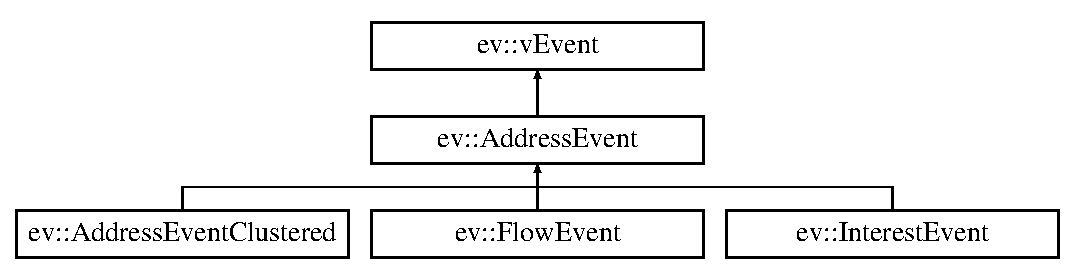
\includegraphics[height=3.000000cm]{classev_1_1AddressEvent}
\end{center}
\end{figure}
\subsection*{Public Member Functions}
\begin{DoxyCompactItemize}
\item 
virtual std\+::string {\bfseries get\+Type} () const \hypertarget{classev_1_1AddressEvent_a11b6638defa5a38a42863002feccfcad}{}\label{classev_1_1AddressEvent_a11b6638defa5a38a42863002feccfcad}

\item 
int {\bfseries get\+Channel} () const \hypertarget{classev_1_1AddressEvent_a88038634ab480b42ac1f056abe004b5d}{}\label{classev_1_1AddressEvent_a88038634ab480b42ac1f056abe004b5d}

\item 
int {\bfseries get\+Polarity} () const \hypertarget{classev_1_1AddressEvent_add01928ce43dabc632bf91d18df09ed1}{}\label{classev_1_1AddressEvent_add01928ce43dabc632bf91d18df09ed1}

\item 
int {\bfseries getX} () const \hypertarget{classev_1_1AddressEvent_a1fd05781c5ea725826bed3f4ede0bc76}{}\label{classev_1_1AddressEvent_a1fd05781c5ea725826bed3f4ede0bc76}

\item 
int {\bfseries getY} () const \hypertarget{classev_1_1AddressEvent_ae382769a1bbb5429264aa56b34aebc77}{}\label{classev_1_1AddressEvent_ae382769a1bbb5429264aa56b34aebc77}

\item 
void {\bfseries set\+Channel} (const int channel)\hypertarget{classev_1_1AddressEvent_a50e188b1c5702cab67a2175b81c32767}{}\label{classev_1_1AddressEvent_a50e188b1c5702cab67a2175b81c32767}

\item 
void {\bfseries set\+Polarity} (const int polarity)\hypertarget{classev_1_1AddressEvent_a066b1e90b4d7faeaf68fa20bd6e0d3fa}{}\label{classev_1_1AddressEvent_a066b1e90b4d7faeaf68fa20bd6e0d3fa}

\item 
void {\bfseries setX} (const int x)\hypertarget{classev_1_1AddressEvent_aa99a38f1505796132e537cc3e54c7445}{}\label{classev_1_1AddressEvent_aa99a38f1505796132e537cc3e54c7445}

\item 
void {\bfseries setY} (const int y)\hypertarget{classev_1_1AddressEvent_abb2bb72a69c5241d0e293957a73135f6}{}\label{classev_1_1AddressEvent_abb2bb72a69c5241d0e293957a73135f6}

\item 
{\bfseries Address\+Event} (const \hyperlink{classev_1_1vEvent}{v\+Event} \&event)\hypertarget{classev_1_1AddressEvent_acafeb45e4b444a41e7aa50c15735da14}{}\label{classev_1_1AddressEvent_acafeb45e4b444a41e7aa50c15735da14}

\item 
\hyperlink{classev_1_1vEvent}{v\+Event} \& {\bfseries operator=} (const \hyperlink{classev_1_1vEvent}{v\+Event} \&event)\hypertarget{classev_1_1AddressEvent_a2cf6648bb5f36e32e2e6ec9a952fd40a}{}\label{classev_1_1AddressEvent_a2cf6648bb5f36e32e2e6ec9a952fd40a}

\item 
virtual \hyperlink{classev_1_1vEvent}{v\+Event} $\ast$ {\bfseries clone} ()\hypertarget{classev_1_1AddressEvent_ae27d52f5a882c509541e210581530428}{}\label{classev_1_1AddressEvent_ae27d52f5a882c509541e210581530428}

\item 
bool {\bfseries operator==} (const \hyperlink{classev_1_1AddressEvent}{Address\+Event} \&event)\hypertarget{classev_1_1AddressEvent_a68943a097a59e47f627aa5ca8831e1de}{}\label{classev_1_1AddressEvent_a68943a097a59e47f627aa5ca8831e1de}

\item 
bool {\bfseries operator==} (const \hyperlink{classev_1_1vEvent}{v\+Event} \&event)\hypertarget{classev_1_1AddressEvent_ac2a1abf4ea7344ac0334216deffad02e}{}\label{classev_1_1AddressEvent_ac2a1abf4ea7344ac0334216deffad02e}

\item 
virtual void {\bfseries encode} (yarp\+::os\+::\+Bottle \&b) const \hypertarget{classev_1_1AddressEvent_a38b726cef241624c31312a3eb1f46730}{}\label{classev_1_1AddressEvent_a38b726cef241624c31312a3eb1f46730}

\item 
yarp\+::os\+::\+Property {\bfseries get\+Content} () const \hypertarget{classev_1_1AddressEvent_ad235efba4a6bd3fc79b853ecefad88c9}{}\label{classev_1_1AddressEvent_ad235efba4a6bd3fc79b853ecefad88c9}

\item 
virtual bool {\bfseries decode} (const yarp\+::os\+::\+Bottle \&packet, int \&pos)\hypertarget{classev_1_1AddressEvent_a91d805c2aeb136bb23e4da04e29d98b1}{}\label{classev_1_1AddressEvent_a91d805c2aeb136bb23e4da04e29d98b1}

\item 
virtual int {\bfseries n\+Bytes\+Coded} () const \hypertarget{classev_1_1AddressEvent_a8ffbd1a9a65ae8e0ae311201265e0fe7}{}\label{classev_1_1AddressEvent_a8ffbd1a9a65ae8e0ae311201265e0fe7}

\end{DoxyCompactItemize}
\subsection*{Protected Attributes}
\begin{DoxyCompactItemize}
\item 
unsigned int {\bfseries x}\+:10\hypertarget{classev_1_1AddressEvent_ab6015dc7a789cb6ff7546c47d58829bf}{}\label{classev_1_1AddressEvent_ab6015dc7a789cb6ff7546c47d58829bf}

\item 
unsigned int {\bfseries y}\+:10\hypertarget{classev_1_1AddressEvent_a2e6918d9a0c935c2424e8096ed610c6f}{}\label{classev_1_1AddressEvent_a2e6918d9a0c935c2424e8096ed610c6f}

\item 
unsigned int {\bfseries channel}\+:1\hypertarget{classev_1_1AddressEvent_ab96b9ac3a42cf1d69859f1edbea9cc7f}{}\label{classev_1_1AddressEvent_ab96b9ac3a42cf1d69859f1edbea9cc7f}

\item 
unsigned int {\bfseries polarity}\+:1\hypertarget{classev_1_1AddressEvent_a79bbcea834183012aa39e9d4b2c594ed}{}\label{classev_1_1AddressEvent_a79bbcea834183012aa39e9d4b2c594ed}

\end{DoxyCompactItemize}


The documentation for this class was generated from the following files\+:\begin{DoxyCompactItemize}
\item 
/home/aglover/workspace/projects/event-\/driven/libraries/include/i\+Cub/eventdriven/v\+Codec.\+h\item 
/home/aglover/workspace/projects/event-\/driven/libraries/src/v\+Codec.\+cpp\end{DoxyCompactItemize}

\hypertarget{classev_1_1AddressEventClustered}{}\section{ev\+:\+:Address\+Event\+Clustered Class Reference}
\label{classev_1_1AddressEventClustered}\index{ev\+::\+Address\+Event\+Clustered@{ev\+::\+Address\+Event\+Clustered}}
Inheritance diagram for ev\+:\+:Address\+Event\+Clustered\+:\begin{figure}[H]
\begin{center}
\leavevmode
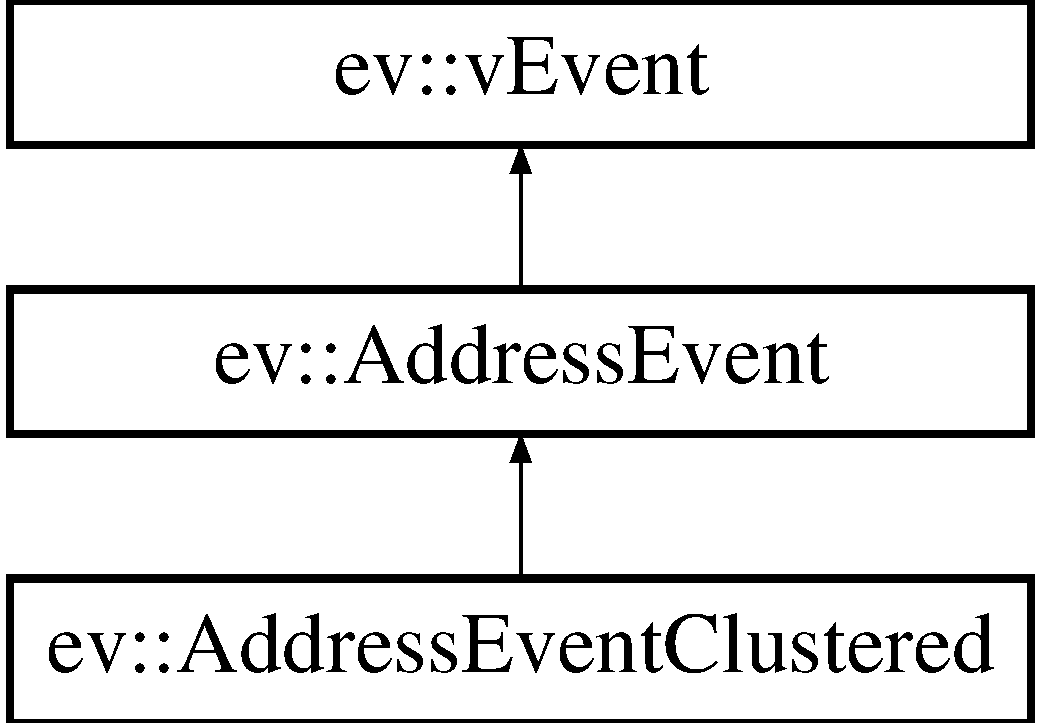
\includegraphics[height=3.000000cm]{classev_1_1AddressEventClustered}
\end{center}
\end{figure}
\subsection*{Public Member Functions}
\begin{DoxyCompactItemize}
\item 
virtual std\+::string {\bfseries get\+Type} () const \hypertarget{classev_1_1AddressEventClustered_aa94f717e6d057e1bf93514ef911bb816}{}\label{classev_1_1AddressEventClustered_aa94f717e6d057e1bf93514ef911bb816}

\item 
int {\bfseries get\+ID} () const \hypertarget{classev_1_1AddressEventClustered_ae67f94b17532d279fe699ce32467d4f3}{}\label{classev_1_1AddressEventClustered_ae67f94b17532d279fe699ce32467d4f3}

\item 
void {\bfseries set\+ID} (const int cl\+ID)\hypertarget{classev_1_1AddressEventClustered_a734fa9597de71f237643bf1e7266f076}{}\label{classev_1_1AddressEventClustered_a734fa9597de71f237643bf1e7266f076}

\item 
{\bfseries Address\+Event\+Clustered} (const \hyperlink{classev_1_1vEvent}{v\+Event} \&event)\hypertarget{classev_1_1AddressEventClustered_a5c446f825d7e0de01b7f55567701b3c8}{}\label{classev_1_1AddressEventClustered_a5c446f825d7e0de01b7f55567701b3c8}

\item 
\hyperlink{classev_1_1vEvent}{v\+Event} \& {\bfseries operator=} (const \hyperlink{classev_1_1vEvent}{v\+Event} \&event)\hypertarget{classev_1_1AddressEventClustered_a095a3e7d00b4399d5f3067d65a573c17}{}\label{classev_1_1AddressEventClustered_a095a3e7d00b4399d5f3067d65a573c17}

\item 
virtual \hyperlink{classev_1_1vEvent}{v\+Event} $\ast$ {\bfseries clone} ()\hypertarget{classev_1_1AddressEventClustered_ae8fb9a80718e4e72902f6577c8646c37}{}\label{classev_1_1AddressEventClustered_ae8fb9a80718e4e72902f6577c8646c37}

\item 
bool {\bfseries operator==} (const \hyperlink{classev_1_1AddressEventClustered}{Address\+Event\+Clustered} \&event)\hypertarget{classev_1_1AddressEventClustered_aa2a96b9c4e98bcfb8e1414d3eed41bb4}{}\label{classev_1_1AddressEventClustered_aa2a96b9c4e98bcfb8e1414d3eed41bb4}

\item 
bool {\bfseries operator==} (const \hyperlink{classev_1_1vEvent}{v\+Event} \&event)\hypertarget{classev_1_1AddressEventClustered_a5060e38f6a55b07cbad61d8fe016c0df}{}\label{classev_1_1AddressEventClustered_a5060e38f6a55b07cbad61d8fe016c0df}

\item 
virtual void {\bfseries encode} (yarp\+::os\+::\+Bottle \&b) const \hypertarget{classev_1_1AddressEventClustered_a969434b89a4120a2f96e2b8d7b36a518}{}\label{classev_1_1AddressEventClustered_a969434b89a4120a2f96e2b8d7b36a518}

\item 
yarp\+::os\+::\+Property {\bfseries get\+Content} () const \hypertarget{classev_1_1AddressEventClustered_aa8e4111a73fb6e209cc1d7a8c84d00f8}{}\label{classev_1_1AddressEventClustered_aa8e4111a73fb6e209cc1d7a8c84d00f8}

\item 
virtual bool {\bfseries decode} (const yarp\+::os\+::\+Bottle \&packet, int \&pos)\hypertarget{classev_1_1AddressEventClustered_ad11d10722ceea22d306199bee7e3f562}{}\label{classev_1_1AddressEventClustered_ad11d10722ceea22d306199bee7e3f562}

\item 
virtual int {\bfseries n\+Bytes\+Coded} () const \hypertarget{classev_1_1AddressEventClustered_ad492d8b43964c80c39a34b657dae8a34}{}\label{classev_1_1AddressEventClustered_ad492d8b43964c80c39a34b657dae8a34}

\end{DoxyCompactItemize}
\subsection*{Protected Attributes}
\begin{DoxyCompactItemize}
\item 
int {\bfseries cl\+ID}\hypertarget{classev_1_1AddressEventClustered_a1a4756c2a181d863d3f577e3f83e8afd}{}\label{classev_1_1AddressEventClustered_a1a4756c2a181d863d3f577e3f83e8afd}

\end{DoxyCompactItemize}


The documentation for this class was generated from the following files\+:\begin{DoxyCompactItemize}
\item 
/home/aglover/workspace/projects/event-\/driven/libraries/include/i\+Cub/eventdriven/v\+Codec.\+h\item 
/home/aglover/workspace/projects/event-\/driven/libraries/src/v\+Codec.\+cpp\end{DoxyCompactItemize}

\hypertarget{structaer}{}\section{aer Struct Reference}
\label{structaer}\index{aer@{aer}}
\subsection*{Public Attributes}
\begin{DoxyCompactItemize}
\item 
u32 {\bfseries timestamp}\hypertarget{structaer_a74e35f1258f6c79df0b88f2544c36b7d}{}\label{structaer_a74e35f1258f6c79df0b88f2544c36b7d}

\item 
u32 {\bfseries address}\hypertarget{structaer_a427837e13cd5ba64e6e70552b6e3e78f}{}\label{structaer_a427837e13cd5ba64e6e70552b6e3e78f}

\end{DoxyCompactItemize}


The documentation for this struct was generated from the following file\+:\begin{DoxyCompactItemize}
\item 
/home/aglover/workspace/projects/event-\/driven/src/hardwareio/aex\+Grabber/include/\hyperlink{device2yarp_8h}{device2yarp.\+h}\end{DoxyCompactItemize}

\hypertarget{classaexGrabberModule}{}\section{aex\+Grabber\+Module Class Reference}
\label{classaexGrabberModule}\index{aex\+Grabber\+Module@{aex\+Grabber\+Module}}
Inheritance diagram for aex\+Grabber\+Module\+:\begin{figure}[H]
\begin{center}
\leavevmode
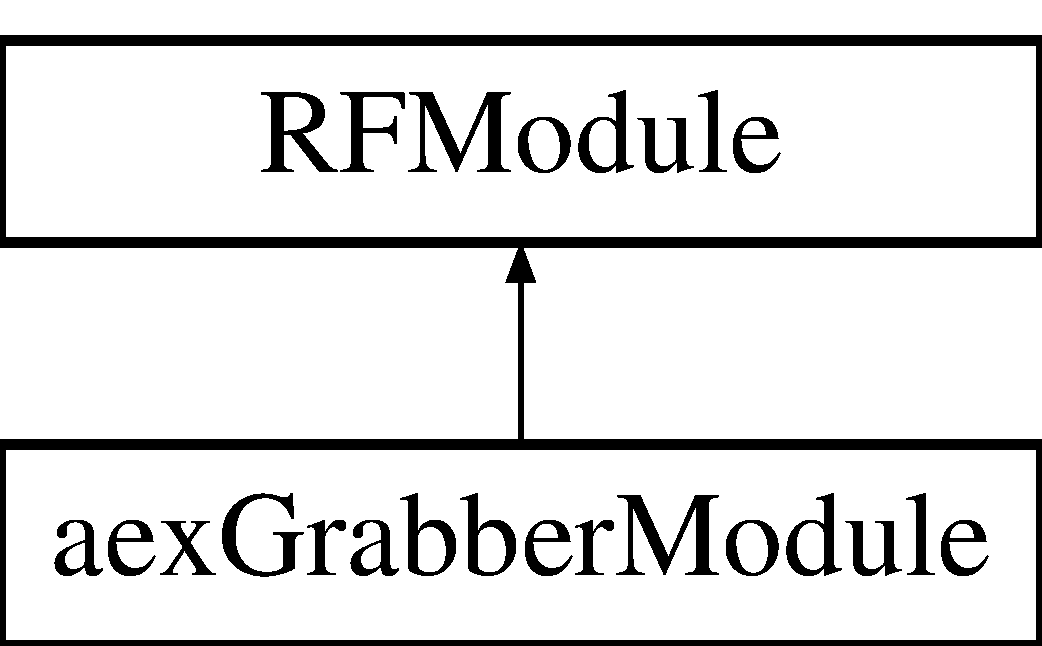
\includegraphics[height=2.000000cm]{classaexGrabberModule}
\end{center}
\end{figure}
\subsection*{Public Member Functions}
\begin{DoxyCompactItemize}
\item 
bool {\bfseries configure} (yarp\+::os\+::\+Resource\+Finder \&rf)\hypertarget{classaexGrabberModule_a7654bd490ccdd31ffc5de4e5d85789f3}{}\label{classaexGrabberModule_a7654bd490ccdd31ffc5de4e5d85789f3}

\item 
bool {\bfseries interrupt\+Module} ()\hypertarget{classaexGrabberModule_a349f07e43758979d9f7e520dd25ba868}{}\label{classaexGrabberModule_a349f07e43758979d9f7e520dd25ba868}

\item 
bool {\bfseries close} ()\hypertarget{classaexGrabberModule_ac032595742ec7bfdd3d6788436572aca}{}\label{classaexGrabberModule_ac032595742ec7bfdd3d6788436572aca}

\item 
bool {\bfseries respond} (const yarp\+::os\+::\+Bottle \&command, yarp\+::os\+::\+Bottle \&reply)\hypertarget{classaexGrabberModule_a18cadf0f324c5dbb7a8d9acfb767ffc0}{}\label{classaexGrabberModule_a18cadf0f324c5dbb7a8d9acfb767ffc0}

\item 
double {\bfseries get\+Period} ()\hypertarget{classaexGrabberModule_a06d7548efce14fbb37945f5640ca029a}{}\label{classaexGrabberModule_a06d7548efce14fbb37945f5640ca029a}

\item 
bool {\bfseries update\+Module} ()\hypertarget{classaexGrabberModule_ae08d72931d6f5283092228dab867d92e}{}\label{classaexGrabberModule_ae08d72931d6f5283092228dab867d92e}

\end{DoxyCompactItemize}


The documentation for this class was generated from the following files\+:\begin{DoxyCompactItemize}
\item 
/home/aglover/workspace/projects/event-\/driven/src/hardwareio/aex\+Grabber/include/aex\+Grabber\+Module.\+h\item 
/home/aglover/workspace/projects/event-\/driven/src/hardwareio/aex\+Grabber/src/\hyperlink{aexGrabberModule_8cpp}{aex\+Grabber\+Module.\+cpp}\end{DoxyCompactItemize}

\hypertarget{structatom}{}\section{atom Struct Reference}
\label{structatom}\index{atom@{atom}}
\subsection*{Public Attributes}
\begin{DoxyCompactItemize}
\item 
u32 {\bfseries data}\hypertarget{structatom_a54c9c4d5af5fc3f2ca8f14f05917c197}{}\label{structatom_a54c9c4d5af5fc3f2ca8f14f05917c197}

\end{DoxyCompactItemize}


The documentation for this struct was generated from the following file\+:\begin{DoxyCompactItemize}
\item 
/home/aglover/workspace/projects/event-\/driven/src/hardwareio/aex\+Grabber/include/\hyperlink{device2yarp_8h}{device2yarp.\+h}\end{DoxyCompactItemize}

\hypertarget{classBlobTracker}{}\section{Blob\+Tracker Class Reference}
\label{classBlobTracker}\index{Blob\+Tracker@{Blob\+Tracker}}
\subsection*{Public Member Functions}
\begin{DoxyCompactItemize}
\item 
bool {\bfseries initialise\+Position} (double x, double y)\hypertarget{classBlobTracker_ac3dbde755642d5e9cf179123823a8eec}{}\label{classBlobTracker_ac3dbde755642d5e9cf179123823a8eec}

\item 
bool {\bfseries initialise\+Shape} (double sigX, double sig\+Y2, double sig\+XY, double alpha\+\_\+pos, double alpha\+\_\+shape, bool fix)\hypertarget{classBlobTracker_a29990e53b163a720f284978b97a6d723}{}\label{classBlobTracker_a29990e53b163a720f284978b97a6d723}

\item 
double {\bfseries dist2event} (int ev\+\_\+x, int ev\+\_\+y)\hypertarget{classBlobTracker_a873c6f0932845537163a5b80605ac599}{}\label{classBlobTracker_a873c6f0932845537163a5b80605ac599}

\item 
double {\bfseries compute\+\_\+p} (int ev\+\_\+x, int ev\+\_\+y)\hypertarget{classBlobTracker_abfe11c1db8b5c9634ec9f5ba86f379d9}{}\label{classBlobTracker_abfe11c1db8b5c9634ec9f5ba86f379d9}

\item 
bool {\bfseries add\+Activity} (int x, int y, unsigned long int ts, double Tact, double Tevent)\hypertarget{classBlobTracker_ab84953899ecee068e63a8f1a89fe7dd8}{}\label{classBlobTracker_ab84953899ecee068e63a8f1a89fe7dd8}

\item 
bool {\bfseries decay\+Activity} (int dt, double tau, double Tinact, double Tfree)\hypertarget{classBlobTracker_af410be534735ad33bafc259d70316a54}{}\label{classBlobTracker_af410be534735ad33bafc259d70316a54}

\item 
void {\bfseries cluster\+Spiked} ()\hypertarget{classBlobTracker_af7a07b561d9516ab480632667672e7ed}{}\label{classBlobTracker_af7a07b561d9516ab480632667672e7ed}

\item 
void {\bfseries is\+No\+Longer\+Free} ()\hypertarget{classBlobTracker_ad22b6a8aaf647e71b57fba25f9f419d1}{}\label{classBlobTracker_ad22b6a8aaf647e71b57fba25f9f419d1}

\item 
bool {\bfseries is\+\_\+active} ()\hypertarget{classBlobTracker_af0cd5a8da431251197c88560c919d89d}{}\label{classBlobTracker_af0cd5a8da431251197c88560c919d89d}

\item 
bool {\bfseries is\+\_\+on} ()\hypertarget{classBlobTracker_a8f18821eb105ce6e95d05e4cc4e3a3aa}{}\label{classBlobTracker_a8f18821eb105ce6e95d05e4cc4e3a3aa}

\item 
bool {\bfseries is\+Free} ()\hypertarget{classBlobTracker_a21f9c5029c220f71e7442a8b068431b7}{}\label{classBlobTracker_a21f9c5029c220f71e7442a8b068431b7}

\item 
double {\bfseries get\+\_\+sigx2} ()\hypertarget{classBlobTracker_ab42f73b98cb1885cdd162148ace8bf23}{}\label{classBlobTracker_ab42f73b98cb1885cdd162148ace8bf23}

\item 
double {\bfseries get\+\_\+sigy2} ()\hypertarget{classBlobTracker_a6cc4fcfc6ade9a856dc7ba502531adf5}{}\label{classBlobTracker_a6cc4fcfc6ade9a856dc7ba502531adf5}

\item 
double {\bfseries get\+\_\+sigxy} ()\hypertarget{classBlobTracker_aeb6aed3ccd9793682b005127fab2bffd}{}\label{classBlobTracker_aeb6aed3ccd9793682b005127fab2bffd}

\item 
int {\bfseries get\+\_\+x} ()\hypertarget{classBlobTracker_aa20dbabdbbfabb44301d18bc59881488}{}\label{classBlobTracker_aa20dbabdbbfabb44301d18bc59881488}

\item 
int {\bfseries get\+\_\+y} ()\hypertarget{classBlobTracker_a2d78cea632f8f9fa4b325c575b9b49d9}{}\label{classBlobTracker_a2d78cea632f8f9fa4b325c575b9b49d9}

\item 
double {\bfseries get\+\_\+vx} ()\hypertarget{classBlobTracker_a339a2cdbf0e3af39241abc7dac115f6c}{}\label{classBlobTracker_a339a2cdbf0e3af39241abc7dac115f6c}

\item 
double {\bfseries get\+\_\+vy} ()\hypertarget{classBlobTracker_a99050a07f515b524837a3977e9c53a9c}{}\label{classBlobTracker_a99050a07f515b524837a3977e9c53a9c}

\item 
double {\bfseries get\+\_\+act} ()\hypertarget{classBlobTracker_a8b59d7b66e32c3c55486f7ef7446fbde}{}\label{classBlobTracker_a8b59d7b66e32c3c55486f7ef7446fbde}

\end{DoxyCompactItemize}
\subsection*{Protected Types}
\begin{DoxyCompactItemize}
\item 
enum {\bfseries State} \{ {\bfseries Active}, 
{\bfseries Inactive}, 
{\bfseries Free}
 \}\hypertarget{classBlobTracker_a7e8d5dcd8736e3ae2a1c448a36e3516f}{}\label{classBlobTracker_a7e8d5dcd8736e3ae2a1c448a36e3516f}

\end{DoxyCompactItemize}
\subsection*{Protected Attributes}
\begin{DoxyCompactItemize}
\item 
State {\bfseries state\+\_\+}\hypertarget{classBlobTracker_ad96c96edcf8e9b2155aba3c39d128249}{}\label{classBlobTracker_ad96c96edcf8e9b2155aba3c39d128249}

\item 
double {\bfseries cen\+\_\+x\+\_\+}\hypertarget{classBlobTracker_a93b360b9499b9a77c7da2eb0b264d8af}{}\label{classBlobTracker_a93b360b9499b9a77c7da2eb0b264d8af}

\item 
double {\bfseries cen\+\_\+y\+\_\+}\hypertarget{classBlobTracker_ab5eaa89cfedfb25fc0881009cefdbea4}{}\label{classBlobTracker_ab5eaa89cfedfb25fc0881009cefdbea4}

\item 
double {\bfseries sig\+\_\+x2\+\_\+}\hypertarget{classBlobTracker_a90039cb4599ff8cf137d0b0a9b89801e}{}\label{classBlobTracker_a90039cb4599ff8cf137d0b0a9b89801e}

\item 
double {\bfseries sig\+\_\+y2\+\_\+}\hypertarget{classBlobTracker_a8fa7fa36db3faed93d94b30bd50449e1}{}\label{classBlobTracker_a8fa7fa36db3faed93d94b30bd50449e1}

\item 
double {\bfseries sig\+\_\+xy\+\_\+}\hypertarget{classBlobTracker_af7c64be12d9aeee877adc6027e57dc31}{}\label{classBlobTracker_af7c64be12d9aeee877adc6027e57dc31}

\item 
double {\bfseries v\+LastX}\hypertarget{classBlobTracker_a37789b44e5e478a237580a3e168bd496}{}\label{classBlobTracker_a37789b44e5e478a237580a3e168bd496}

\item 
double {\bfseries v\+LastY}\hypertarget{classBlobTracker_ae836b9dd8d830ba8f6ccb6ea2f80e313}{}\label{classBlobTracker_ae836b9dd8d830ba8f6ccb6ea2f80e313}

\item 
double {\bfseries vx\+\_\+}\hypertarget{classBlobTracker_a98a091e1f3a0e16a71ff6602079c9c23}{}\label{classBlobTracker_a98a091e1f3a0e16a71ff6602079c9c23}

\item 
double {\bfseries vy\+\_\+}\hypertarget{classBlobTracker_a5b41c1c66d14c8b794b314ba204a93bd}{}\label{classBlobTracker_a5b41c1c66d14c8b794b314ba204a93bd}

\item 
double {\bfseries alpha\+\_\+pos\+\_\+}\hypertarget{classBlobTracker_ae10a65c546bfa9ed53d341a46080f53f}{}\label{classBlobTracker_ae10a65c546bfa9ed53d341a46080f53f}

\item 
double {\bfseries alpha\+\_\+shape\+\_\+}\hypertarget{classBlobTracker_a5183d2c99bd9dbc6f7170050e5830dea}{}\label{classBlobTracker_a5183d2c99bd9dbc6f7170050e5830dea}

\item 
bool {\bfseries fixed\+\_\+shape\+\_\+}\hypertarget{classBlobTracker_a57841b67cf49324e2ff7b9698897e908}{}\label{classBlobTracker_a57841b67cf49324e2ff7b9698897e908}

\item 
double {\bfseries activity\+\_\+}\hypertarget{classBlobTracker_aaf83587414449f41fa7719f9939c48a8}{}\label{classBlobTracker_aaf83587414449f41fa7719f9939c48a8}

\item 
unsigned long int {\bfseries ts\+\_\+last\+\_\+update\+\_\+}\hypertarget{classBlobTracker_a4084fae015313204286ce98259856467}{}\label{classBlobTracker_a4084fae015313204286ce98259856467}

\end{DoxyCompactItemize}


The documentation for this class was generated from the following files\+:\begin{DoxyCompactItemize}
\item 
/home/aglover/workspace/projects/event-\/driven/src/modules/v\+Cluster/include/blob\+Tracker.\+h\item 
/home/aglover/workspace/projects/event-\/driven/src/modules/v\+Cluster/src/blob\+Tracker.\+cpp\end{DoxyCompactItemize}

\hypertarget{classcircleDisparity}{}\section{circle\+Disparity Class Reference}
\label{classcircleDisparity}\index{circle\+Disparity@{circle\+Disparity}}
Inheritance diagram for circle\+Disparity\+:\begin{figure}[H]
\begin{center}
\leavevmode
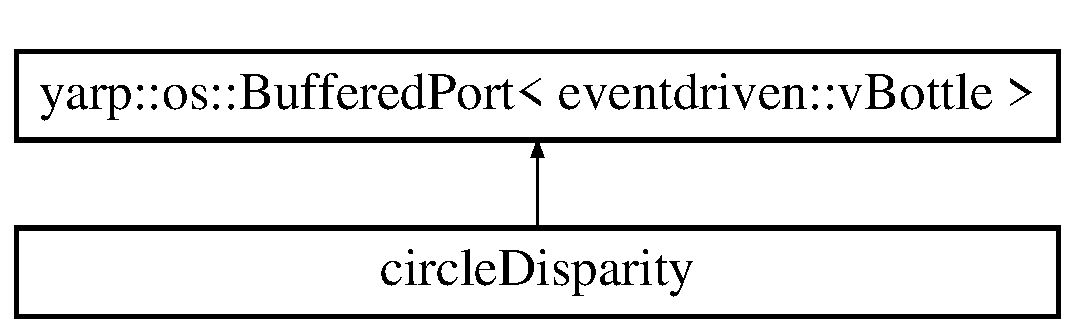
\includegraphics[height=2.000000cm]{classcircleDisparity}
\end{center}
\end{figure}
\subsection*{Public Member Functions}
\begin{DoxyCompactItemize}
\item 
bool {\bfseries open} (const std\+::string \&name, bool strict=false)\hypertarget{classcircleDisparity_a5be77ddfdbb425def639e31b53226687}{}\label{classcircleDisparity_a5be77ddfdbb425def639e31b53226687}

\item 
void {\bfseries close} ()\hypertarget{classcircleDisparity_ac492ff92d6e537bdfcee8aac01413d1f}{}\label{classcircleDisparity_ac492ff92d6e537bdfcee8aac01413d1f}

\item 
void {\bfseries interrupt} ()\hypertarget{classcircleDisparity_a190e0c9fc70997a3925fc1f22d0729ad}{}\label{classcircleDisparity_a190e0c9fc70997a3925fc1f22d0729ad}

\item 
void {\bfseries on\+Read} (eventdriven\+::v\+Bottle \&v\+Bottle\+In)\hypertarget{classcircleDisparity_a3585217994a641d81b2c82d39f3f1f72}{}\label{classcircleDisparity_a3585217994a641d81b2c82d39f3f1f72}

\end{DoxyCompactItemize}


The documentation for this class was generated from the following files\+:\begin{DoxyCompactItemize}
\item 
/home/aglover/workspace/projects/event-\/driven/src/modules/v\+Circle\+Disparity/include/v\+Circle\+Disparity.\+h\item 
/home/aglover/workspace/projects/event-\/driven/src/modules/v\+Circle\+Disparity/src/v\+Circle\+Disparity.\+cpp\end{DoxyCompactItemize}

\hypertarget{classev_1_1ClusterEvent}{}\section{ev\+:\+:Cluster\+Event Class Reference}
\label{classev_1_1ClusterEvent}\index{ev\+::\+Cluster\+Event@{ev\+::\+Cluster\+Event}}
Inheritance diagram for ev\+:\+:Cluster\+Event\+:\begin{figure}[H]
\begin{center}
\leavevmode
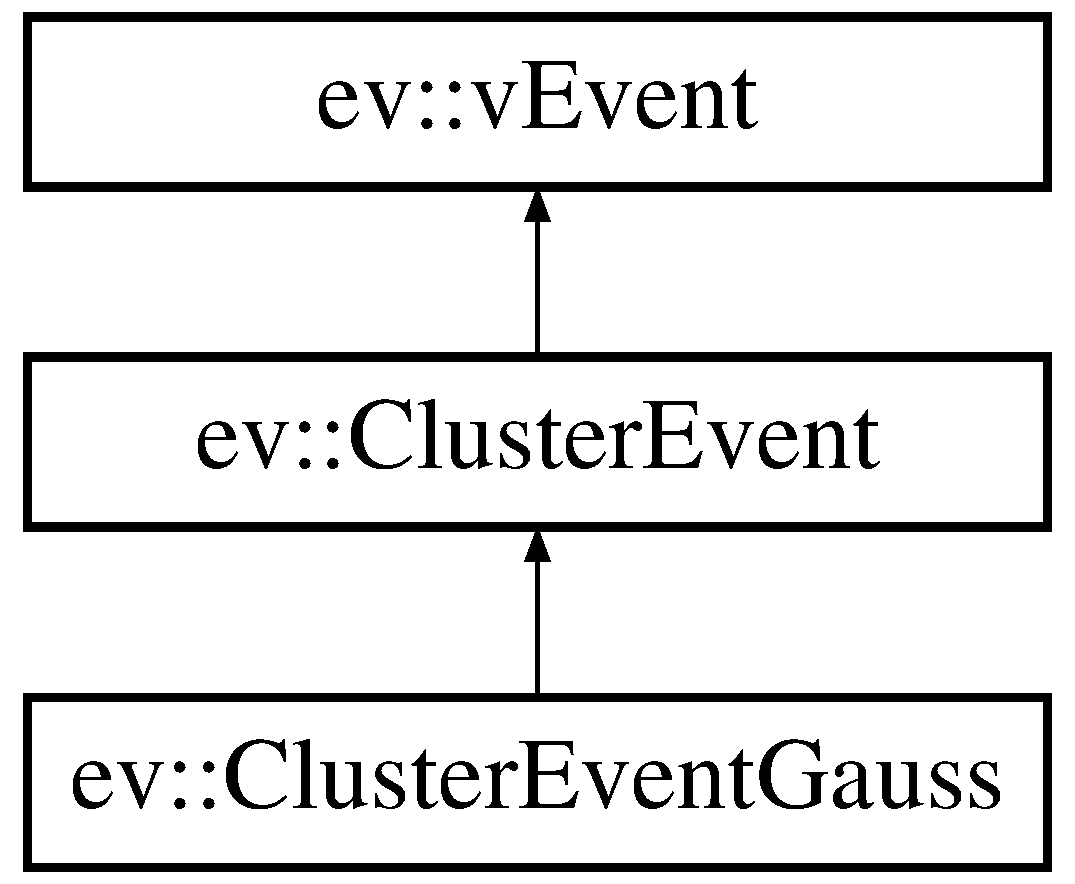
\includegraphics[height=3.000000cm]{classev_1_1ClusterEvent}
\end{center}
\end{figure}
\subsection*{Public Member Functions}
\begin{DoxyCompactItemize}
\item 
virtual std\+::string {\bfseries get\+Type} () const \hypertarget{classev_1_1ClusterEvent_a2b6c1d4d12960ab15433c2dbb57842a2}{}\label{classev_1_1ClusterEvent_a2b6c1d4d12960ab15433c2dbb57842a2}

\item 
int {\bfseries get\+Channel} () const \hypertarget{classev_1_1ClusterEvent_ad43d3e3e1a3f1ccd5aeb648c9e6154c2}{}\label{classev_1_1ClusterEvent_ad43d3e3e1a3f1ccd5aeb648c9e6154c2}

\item 
int {\bfseries get\+ID} () const \hypertarget{classev_1_1ClusterEvent_a007e8b487445ea71d1bff82f3d59fdec}{}\label{classev_1_1ClusterEvent_a007e8b487445ea71d1bff82f3d59fdec}

\item 
int {\bfseries get\+X\+Cog} () const \hypertarget{classev_1_1ClusterEvent_a30e569d0ca23b77e2da9bd4a98b94fc7}{}\label{classev_1_1ClusterEvent_a30e569d0ca23b77e2da9bd4a98b94fc7}

\item 
int {\bfseries get\+Y\+Cog} () const \hypertarget{classev_1_1ClusterEvent_a46e89174921f68a96e45fe61273fac3a}{}\label{classev_1_1ClusterEvent_a46e89174921f68a96e45fe61273fac3a}

\item 
int {\bfseries get\+Polarity} () const \hypertarget{classev_1_1ClusterEvent_a8af0afe7b7c9879f3d3ff721b12d3459}{}\label{classev_1_1ClusterEvent_a8af0afe7b7c9879f3d3ff721b12d3459}

\item 
void {\bfseries set\+Channel} (const int channel)\hypertarget{classev_1_1ClusterEvent_aeabb79032ebd04cd7802cfda38c24389}{}\label{classev_1_1ClusterEvent_aeabb79032ebd04cd7802cfda38c24389}

\item 
void {\bfseries set\+ID} (const int id)\hypertarget{classev_1_1ClusterEvent_a82a500a0a8bfcc84d6a1b46c816d6ea7}{}\label{classev_1_1ClusterEvent_a82a500a0a8bfcc84d6a1b46c816d6ea7}

\item 
void {\bfseries set\+X\+Cog} (const int x\+Cog)\hypertarget{classev_1_1ClusterEvent_a3853aec21b42b82a8fde9b67131a5eee}{}\label{classev_1_1ClusterEvent_a3853aec21b42b82a8fde9b67131a5eee}

\item 
void {\bfseries set\+Y\+Cog} (const int y\+Cog)\hypertarget{classev_1_1ClusterEvent_aa6703fbe78bffbd21ad2bacc9bd3d3b8}{}\label{classev_1_1ClusterEvent_aa6703fbe78bffbd21ad2bacc9bd3d3b8}

\item 
void {\bfseries set\+Polarity} (const int polarity)\hypertarget{classev_1_1ClusterEvent_aacd9f0d278ca277b22ad8db3e8ad67db}{}\label{classev_1_1ClusterEvent_aacd9f0d278ca277b22ad8db3e8ad67db}

\item 
{\bfseries Cluster\+Event} (const \hyperlink{classev_1_1vEvent}{v\+Event} \&event)\hypertarget{classev_1_1ClusterEvent_abe86469c963b2f313c57224a1c8a770d}{}\label{classev_1_1ClusterEvent_abe86469c963b2f313c57224a1c8a770d}

\item 
\hyperlink{classev_1_1vEvent}{v\+Event} \& {\bfseries operator=} (const \hyperlink{classev_1_1vEvent}{v\+Event} \&event)\hypertarget{classev_1_1ClusterEvent_a2849ce0d84c9a8a014d12d1a3d4718d6}{}\label{classev_1_1ClusterEvent_a2849ce0d84c9a8a014d12d1a3d4718d6}

\item 
virtual \hyperlink{classev_1_1vEvent}{v\+Event} $\ast$ {\bfseries clone} ()\hypertarget{classev_1_1ClusterEvent_a32b61af5a3bab167c98fa680694b1dfb}{}\label{classev_1_1ClusterEvent_a32b61af5a3bab167c98fa680694b1dfb}

\item 
bool {\bfseries operator==} (const \hyperlink{classev_1_1ClusterEvent}{Cluster\+Event} \&event)\hypertarget{classev_1_1ClusterEvent_a4ff5207487dde56afec4970d44ab3c80}{}\label{classev_1_1ClusterEvent_a4ff5207487dde56afec4970d44ab3c80}

\item 
bool {\bfseries operator==} (const \hyperlink{classev_1_1vEvent}{v\+Event} \&event)\hypertarget{classev_1_1ClusterEvent_a8c2ddb8563caf4604cca97a9d29510e7}{}\label{classev_1_1ClusterEvent_a8c2ddb8563caf4604cca97a9d29510e7}

\item 
virtual void {\bfseries encode} (yarp\+::os\+::\+Bottle \&b) const \hypertarget{classev_1_1ClusterEvent_ab90a45903498a88369164711e5fc9ba3}{}\label{classev_1_1ClusterEvent_ab90a45903498a88369164711e5fc9ba3}

\item 
yarp\+::os\+::\+Property {\bfseries get\+Content} () const \hypertarget{classev_1_1ClusterEvent_a95be2a982e74b261768d1150fb0fd12d}{}\label{classev_1_1ClusterEvent_a95be2a982e74b261768d1150fb0fd12d}

\item 
virtual bool {\bfseries decode} (const yarp\+::os\+::\+Bottle \&packet, int \&pos)\hypertarget{classev_1_1ClusterEvent_abe3ccfd94ecded904beb4e126e448c9f}{}\label{classev_1_1ClusterEvent_abe3ccfd94ecded904beb4e126e448c9f}

\item 
virtual int {\bfseries n\+Bytes\+Coded} () const \hypertarget{classev_1_1ClusterEvent_ae520fafb58dac573a175abc64eef0467}{}\label{classev_1_1ClusterEvent_ae520fafb58dac573a175abc64eef0467}

\end{DoxyCompactItemize}
\subsection*{Protected Attributes}
\begin{DoxyCompactItemize}
\item 
int {\bfseries id}\+:10\hypertarget{classev_1_1ClusterEvent_a0c4a2883f902f1a2b3fb025a7b8cb37d}{}\label{classev_1_1ClusterEvent_a0c4a2883f902f1a2b3fb025a7b8cb37d}

\item 
unsigned int {\bfseries x\+Cog}\+:10\hypertarget{classev_1_1ClusterEvent_a93c5012538e0a5aaaba820dea4e28c63}{}\label{classev_1_1ClusterEvent_a93c5012538e0a5aaaba820dea4e28c63}

\item 
unsigned int {\bfseries y\+Cog}\+:10\hypertarget{classev_1_1ClusterEvent_ad5b3c4bb36d8aedbeed1624e27bc9716}{}\label{classev_1_1ClusterEvent_ad5b3c4bb36d8aedbeed1624e27bc9716}

\item 
unsigned int {\bfseries polarity}\+:1\hypertarget{classev_1_1ClusterEvent_ad66f5bf0d73bdbd4900609b42b8d0040}{}\label{classev_1_1ClusterEvent_ad66f5bf0d73bdbd4900609b42b8d0040}

\item 
unsigned int {\bfseries channel}\+:1\hypertarget{classev_1_1ClusterEvent_a28dfff3ae10a96e2a49981993be962d1}{}\label{classev_1_1ClusterEvent_a28dfff3ae10a96e2a49981993be962d1}

\end{DoxyCompactItemize}


The documentation for this class was generated from the following files\+:\begin{DoxyCompactItemize}
\item 
/home/aglover/workspace/projects/event-\/driven/libraries/include/i\+Cub/eventdriven/v\+Codec.\+h\item 
/home/aglover/workspace/projects/event-\/driven/libraries/src/v\+Codec.\+cpp\end{DoxyCompactItemize}

\hypertarget{classev_1_1ClusterEventGauss}{}\section{ev\+:\+:Cluster\+Event\+Gauss Class Reference}
\label{classev_1_1ClusterEventGauss}\index{ev\+::\+Cluster\+Event\+Gauss@{ev\+::\+Cluster\+Event\+Gauss}}
Inheritance diagram for ev\+:\+:Cluster\+Event\+Gauss\+:\begin{figure}[H]
\begin{center}
\leavevmode
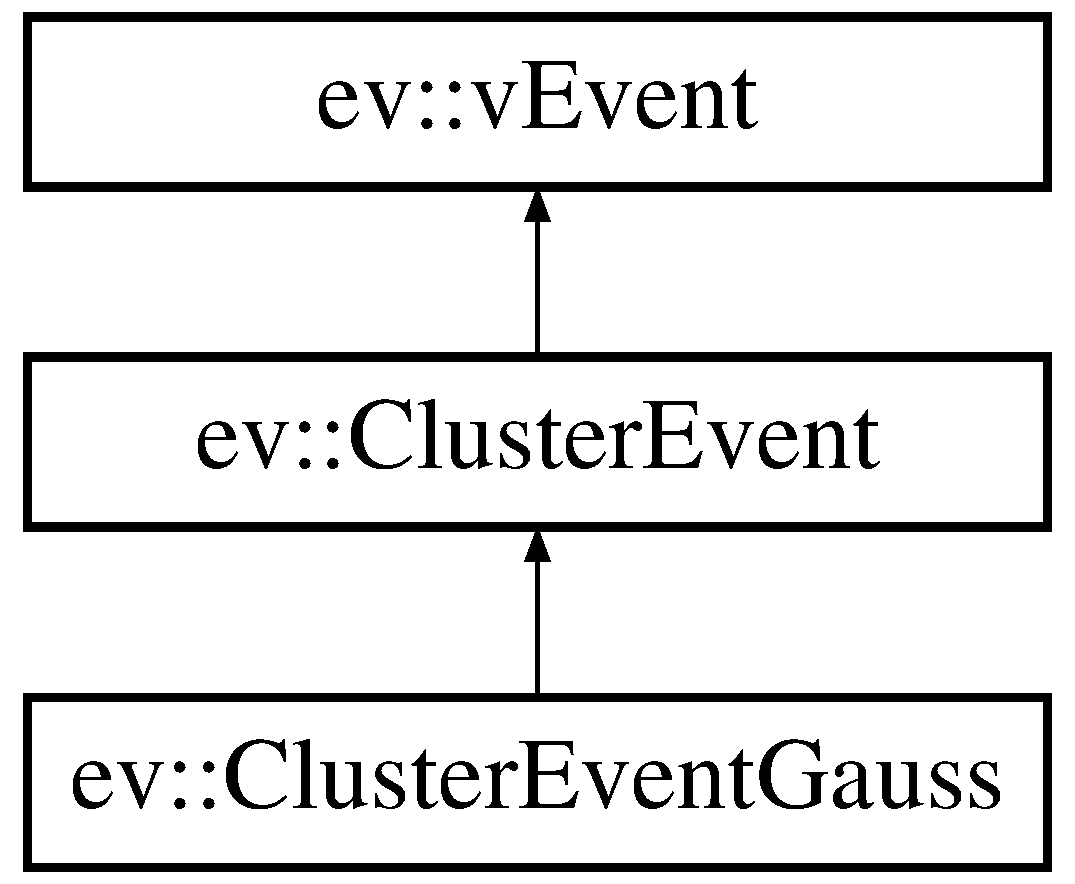
\includegraphics[height=3.000000cm]{classev_1_1ClusterEventGauss}
\end{center}
\end{figure}
\subsection*{Public Member Functions}
\begin{DoxyCompactItemize}
\item 
virtual std\+::string {\bfseries get\+Type} () const \hypertarget{classev_1_1ClusterEventGauss_a1df2453e17843cfce7d83fcb18f6dd0f}{}\label{classev_1_1ClusterEventGauss_a1df2453e17843cfce7d83fcb18f6dd0f}

\item 
int {\bfseries get\+Num\+AE} () const \hypertarget{classev_1_1ClusterEventGauss_a3e2d06634450fb40294c6c826d88dad6}{}\label{classev_1_1ClusterEventGauss_a3e2d06634450fb40294c6c826d88dad6}

\item 
int {\bfseries get\+X\+Sigma2} () const \hypertarget{classev_1_1ClusterEventGauss_aa4898a9304cbf6ed5c3d8883473e9fbf}{}\label{classev_1_1ClusterEventGauss_aa4898a9304cbf6ed5c3d8883473e9fbf}

\item 
int {\bfseries get\+Y\+Sigma2} () const \hypertarget{classev_1_1ClusterEventGauss_ade45d25fe8cd39623bb5f330ae012e6e}{}\label{classev_1_1ClusterEventGauss_ade45d25fe8cd39623bb5f330ae012e6e}

\item 
int {\bfseries get\+X\+Y\+Sigma} () const \hypertarget{classev_1_1ClusterEventGauss_a267d0eb2a46834de84dadd274a08521f}{}\label{classev_1_1ClusterEventGauss_a267d0eb2a46834de84dadd274a08521f}

\item 
int {\bfseries get\+X\+Vel} () const \hypertarget{classev_1_1ClusterEventGauss_a6278b2c5095948a499cb59aa07d79ab0}{}\label{classev_1_1ClusterEventGauss_a6278b2c5095948a499cb59aa07d79ab0}

\item 
int {\bfseries get\+Y\+Vel} () const \hypertarget{classev_1_1ClusterEventGauss_a94dde2e9f7356331e3694b736f8984c7}{}\label{classev_1_1ClusterEventGauss_a94dde2e9f7356331e3694b736f8984c7}

\item 
void {\bfseries set\+Num\+AE} (const int num\+AE)\hypertarget{classev_1_1ClusterEventGauss_a4435e1378dc1431b812917ce0fd78930}{}\label{classev_1_1ClusterEventGauss_a4435e1378dc1431b812917ce0fd78930}

\item 
void {\bfseries set\+X\+Sigma2} (const int x\+Sigma2)\hypertarget{classev_1_1ClusterEventGauss_a14983a1a3c8f4e78f9761d5ed6ebde8d}{}\label{classev_1_1ClusterEventGauss_a14983a1a3c8f4e78f9761d5ed6ebde8d}

\item 
void {\bfseries set\+Y\+Sigma2} (const int y\+Sigma2)\hypertarget{classev_1_1ClusterEventGauss_a9328e993864fa45b077cd5910324e576}{}\label{classev_1_1ClusterEventGauss_a9328e993864fa45b077cd5910324e576}

\item 
void {\bfseries set\+X\+Y\+Sigma} (const int xy\+Sigma)\hypertarget{classev_1_1ClusterEventGauss_ac2e47aad21c85d3336bccd068570e426}{}\label{classev_1_1ClusterEventGauss_ac2e47aad21c85d3336bccd068570e426}

\item 
void {\bfseries set\+X\+Vel} (const int x\+Vel)\hypertarget{classev_1_1ClusterEventGauss_aa0f480bc50e9d30c0b6d0bbfb07a8dc1}{}\label{classev_1_1ClusterEventGauss_aa0f480bc50e9d30c0b6d0bbfb07a8dc1}

\item 
void {\bfseries set\+Y\+Vel} (const int y\+Vel)\hypertarget{classev_1_1ClusterEventGauss_a28c22189446dc2568f36ddf116c112c9}{}\label{classev_1_1ClusterEventGauss_a28c22189446dc2568f36ddf116c112c9}

\item 
{\bfseries Cluster\+Event\+Gauss} (const \hyperlink{classev_1_1vEvent}{v\+Event} \&event)\hypertarget{classev_1_1ClusterEventGauss_a205d1a6b8eadbfaba824a57d770d855a}{}\label{classev_1_1ClusterEventGauss_a205d1a6b8eadbfaba824a57d770d855a}

\item 
\hyperlink{classev_1_1vEvent}{v\+Event} \& {\bfseries operator=} (const \hyperlink{classev_1_1vEvent}{v\+Event} \&event)\hypertarget{classev_1_1ClusterEventGauss_aa201ad35363714787b441bfef6bfaa96}{}\label{classev_1_1ClusterEventGauss_aa201ad35363714787b441bfef6bfaa96}

\item 
virtual \hyperlink{classev_1_1vEvent}{v\+Event} $\ast$ {\bfseries clone} ()\hypertarget{classev_1_1ClusterEventGauss_a4cfabdf0d78cbdf2f803825415bc915d}{}\label{classev_1_1ClusterEventGauss_a4cfabdf0d78cbdf2f803825415bc915d}

\item 
bool {\bfseries operator==} (const \hyperlink{classev_1_1ClusterEventGauss}{Cluster\+Event\+Gauss} \&event)\hypertarget{classev_1_1ClusterEventGauss_a4288d11e77c427b5d57154da51eb7733}{}\label{classev_1_1ClusterEventGauss_a4288d11e77c427b5d57154da51eb7733}

\item 
bool {\bfseries operator==} (const \hyperlink{classev_1_1vEvent}{v\+Event} \&event)\hypertarget{classev_1_1ClusterEventGauss_a2e1b7c1a5a2ba3083cc9ece2dbebe21e}{}\label{classev_1_1ClusterEventGauss_a2e1b7c1a5a2ba3083cc9ece2dbebe21e}

\item 
virtual void {\bfseries encode} (yarp\+::os\+::\+Bottle \&b) const \hypertarget{classev_1_1ClusterEventGauss_aa54b0aba37f5a1f7aa3f77458b4d0843}{}\label{classev_1_1ClusterEventGauss_aa54b0aba37f5a1f7aa3f77458b4d0843}

\item 
yarp\+::os\+::\+Property {\bfseries get\+Content} () const \hypertarget{classev_1_1ClusterEventGauss_aa707d8caffd6d16d518791a3534249e3}{}\label{classev_1_1ClusterEventGauss_aa707d8caffd6d16d518791a3534249e3}

\item 
virtual bool {\bfseries decode} (const yarp\+::os\+::\+Bottle \&packet, int \&pos)\hypertarget{classev_1_1ClusterEventGauss_a7dc887813031611b707e5ace62bab222}{}\label{classev_1_1ClusterEventGauss_a7dc887813031611b707e5ace62bab222}

\item 
virtual int {\bfseries n\+Bytes\+Coded} () const \hypertarget{classev_1_1ClusterEventGauss_aee82fc72b8f35ec88df2e2ddab7a6674}{}\label{classev_1_1ClusterEventGauss_aee82fc72b8f35ec88df2e2ddab7a6674}

\end{DoxyCompactItemize}
\subsection*{Protected Attributes}
\begin{DoxyCompactItemize}
\item 
unsigned int {\bfseries num\+AE}\+:16\hypertarget{classev_1_1ClusterEventGauss_ad33637c7c7648f7f75a5687cb3dc9f10}{}\label{classev_1_1ClusterEventGauss_ad33637c7c7648f7f75a5687cb3dc9f10}

\item 
unsigned int {\bfseries xy\+Sigma}\+:16\hypertarget{classev_1_1ClusterEventGauss_adafdbc89273fdfac859451c96228c3d0}{}\label{classev_1_1ClusterEventGauss_adafdbc89273fdfac859451c96228c3d0}

\item 
unsigned int {\bfseries x\+Sigma2}\+:16\hypertarget{classev_1_1ClusterEventGauss_a949838037074552acbf68e79774e4d0d}{}\label{classev_1_1ClusterEventGauss_a949838037074552acbf68e79774e4d0d}

\item 
unsigned int {\bfseries y\+Sigma2}\+:16\hypertarget{classev_1_1ClusterEventGauss_ab59726c59d3504d60b9561392d4d3536}{}\label{classev_1_1ClusterEventGauss_ab59726c59d3504d60b9561392d4d3536}

\item 
int {\bfseries x\+Vel}\+:16\hypertarget{classev_1_1ClusterEventGauss_a1656c00217f8e7413da96fb63586c533}{}\label{classev_1_1ClusterEventGauss_a1656c00217f8e7413da96fb63586c533}

\item 
int {\bfseries y\+Vel}\+:16\hypertarget{classev_1_1ClusterEventGauss_a94890d974aad5dc36181e35a462ae997}{}\label{classev_1_1ClusterEventGauss_a94890d974aad5dc36181e35a462ae997}

\end{DoxyCompactItemize}


The documentation for this class was generated from the following files\+:\begin{DoxyCompactItemize}
\item 
/home/aglover/workspace/projects/event-\/driven/libraries/include/i\+Cub/eventdriven/v\+Codec.\+h\item 
/home/aglover/workspace/projects/event-\/driven/libraries/src/v\+Codec.\+cpp\end{DoxyCompactItemize}

\hypertarget{classev_1_1CollisionEvent}{}\section{ev\+:\+:Collision\+Event Class Reference}
\label{classev_1_1CollisionEvent}\index{ev\+::\+Collision\+Event@{ev\+::\+Collision\+Event}}
Inheritance diagram for ev\+:\+:Collision\+Event\+:\begin{figure}[H]
\begin{center}
\leavevmode
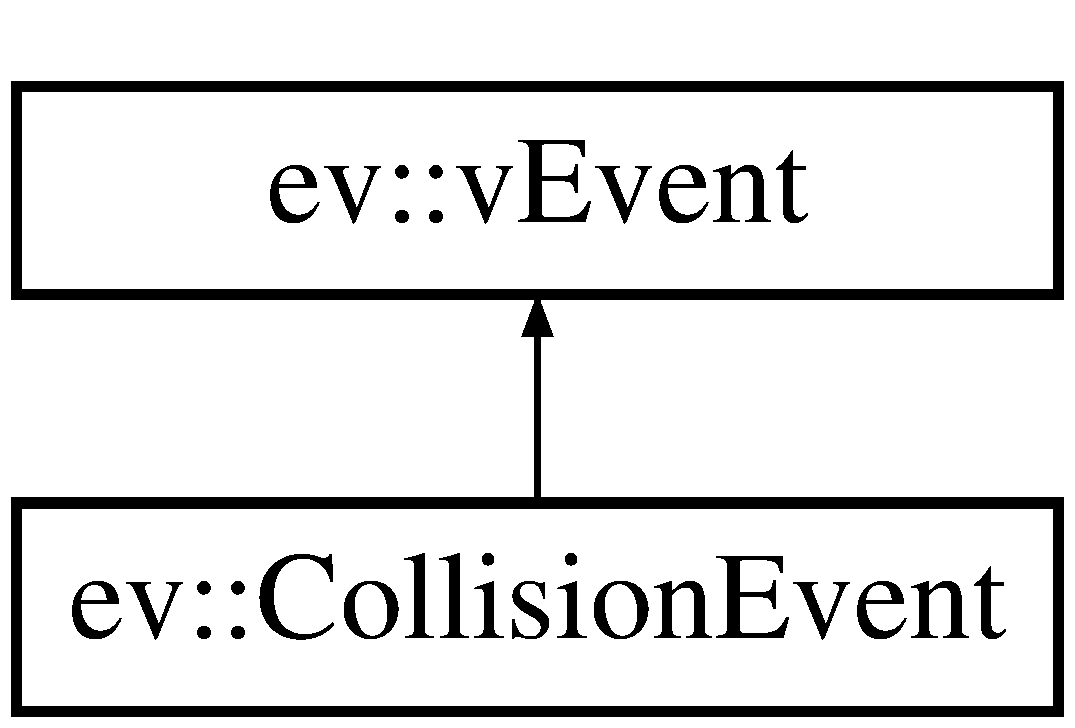
\includegraphics[height=2.000000cm]{classev_1_1CollisionEvent}
\end{center}
\end{figure}
\subsection*{Public Member Functions}
\begin{DoxyCompactItemize}
\item 
virtual std\+::string {\bfseries get\+Type} () const \hypertarget{classev_1_1CollisionEvent_a8c3294310e3f51afbea28abab00b8e3b}{}\label{classev_1_1CollisionEvent_a8c3294310e3f51afbea28abab00b8e3b}

\item 
void {\bfseries setX} (unsigned int x)\hypertarget{classev_1_1CollisionEvent_a3921f015acddf510b6a317a0b10e9f15}{}\label{classev_1_1CollisionEvent_a3921f015acddf510b6a317a0b10e9f15}

\item 
void {\bfseries setY} (unsigned int y)\hypertarget{classev_1_1CollisionEvent_aa9dc1d6e5b9aa67a0b7b502913cee89b}{}\label{classev_1_1CollisionEvent_aa9dc1d6e5b9aa67a0b7b502913cee89b}

\item 
void {\bfseries set\+Channel} (unsigned int channel)\hypertarget{classev_1_1CollisionEvent_abb4121aa9f67570c6ac93289aad7279b}{}\label{classev_1_1CollisionEvent_abb4121aa9f67570c6ac93289aad7279b}

\item 
void {\bfseries set\+Clid1} (unsigned int clid1)\hypertarget{classev_1_1CollisionEvent_a341cee724f0d5a9992454ee1ac1cdd49}{}\label{classev_1_1CollisionEvent_a341cee724f0d5a9992454ee1ac1cdd49}

\item 
void {\bfseries set\+Clid2} (unsigned int clid2)\hypertarget{classev_1_1CollisionEvent_a5b081b2e35cdc3c30f65479c9e5718ee}{}\label{classev_1_1CollisionEvent_a5b081b2e35cdc3c30f65479c9e5718ee}

\item 
unsigned char {\bfseries getX} ()\hypertarget{classev_1_1CollisionEvent_aa20ffbfb15877d44765138595fed0c45}{}\label{classev_1_1CollisionEvent_aa20ffbfb15877d44765138595fed0c45}

\item 
unsigned char {\bfseries getY} ()\hypertarget{classev_1_1CollisionEvent_a08a6c9661d7e2e67b374705c36e086d7}{}\label{classev_1_1CollisionEvent_a08a6c9661d7e2e67b374705c36e086d7}

\item 
virtual int {\bfseries get\+Channel} ()\hypertarget{classev_1_1CollisionEvent_af70a6531452ad00760d46c223a34adf8}{}\label{classev_1_1CollisionEvent_af70a6531452ad00760d46c223a34adf8}

\item 
unsigned char {\bfseries get\+Clid1} ()\hypertarget{classev_1_1CollisionEvent_a921edf40bcb422c118223ca253546e33}{}\label{classev_1_1CollisionEvent_a921edf40bcb422c118223ca253546e33}

\item 
unsigned char {\bfseries get\+Clid2} ()\hypertarget{classev_1_1CollisionEvent_aed04e522dacc30f00e6bbd9aaf686e7a}{}\label{classev_1_1CollisionEvent_aed04e522dacc30f00e6bbd9aaf686e7a}

\item 
{\bfseries Collision\+Event} (const \hyperlink{classev_1_1vEvent}{v\+Event} \&event)\hypertarget{classev_1_1CollisionEvent_a084e588b665cef19268db944df641673}{}\label{classev_1_1CollisionEvent_a084e588b665cef19268db944df641673}

\item 
\hyperlink{classev_1_1vEvent}{v\+Event} \& {\bfseries operator=} (const \hyperlink{classev_1_1vEvent}{v\+Event} \&event)\hypertarget{classev_1_1CollisionEvent_ad1366b88a650bc8866c3ea207aaf44f9}{}\label{classev_1_1CollisionEvent_ad1366b88a650bc8866c3ea207aaf44f9}

\item 
virtual \hyperlink{classev_1_1vEvent}{v\+Event} $\ast$ {\bfseries clone} ()\hypertarget{classev_1_1CollisionEvent_a7445babc8f66f032f95f52c93913311d}{}\label{classev_1_1CollisionEvent_a7445babc8f66f032f95f52c93913311d}

\item 
bool {\bfseries operator==} (const \hyperlink{classev_1_1CollisionEvent}{Collision\+Event} \&event)\hypertarget{classev_1_1CollisionEvent_a5ad8c1c4b50ff8f537b3911240acc72e}{}\label{classev_1_1CollisionEvent_a5ad8c1c4b50ff8f537b3911240acc72e}

\item 
bool {\bfseries operator==} (const \hyperlink{classev_1_1vEvent}{v\+Event} \&event)\hypertarget{classev_1_1CollisionEvent_ad0748e788fe1130d27bc7e2b349fe887}{}\label{classev_1_1CollisionEvent_ad0748e788fe1130d27bc7e2b349fe887}

\item 
virtual void {\bfseries encode} (yarp\+::os\+::\+Bottle \&b) const \hypertarget{classev_1_1CollisionEvent_a58b105333fa3cb719bf4d37fb5147893}{}\label{classev_1_1CollisionEvent_a58b105333fa3cb719bf4d37fb5147893}

\item 
yarp\+::os\+::\+Property {\bfseries get\+Content} () const \hypertarget{classev_1_1CollisionEvent_aa02a65fbe5e0fa02ba5f5ca0f368991b}{}\label{classev_1_1CollisionEvent_aa02a65fbe5e0fa02ba5f5ca0f368991b}

\item 
virtual bool {\bfseries decode} (const yarp\+::os\+::\+Bottle \&packet, int \&pos)\hypertarget{classev_1_1CollisionEvent_aacd61e2522dc199f9797673d5dae408c}{}\label{classev_1_1CollisionEvent_aacd61e2522dc199f9797673d5dae408c}

\item 
virtual int {\bfseries n\+Bytes\+Coded} () const \hypertarget{classev_1_1CollisionEvent_ac2fbae11a37b170bedb0d983f669dd17}{}\label{classev_1_1CollisionEvent_ac2fbae11a37b170bedb0d983f669dd17}

\end{DoxyCompactItemize}
\subsection*{Protected Attributes}
\begin{DoxyCompactItemize}
\item 
unsigned int {\bfseries x}\+:10\hypertarget{classev_1_1CollisionEvent_ab8dfa32e6701e2abcf6601d3a4618547}{}\label{classev_1_1CollisionEvent_ab8dfa32e6701e2abcf6601d3a4618547}

\item 
unsigned int {\bfseries y}\+:10\hypertarget{classev_1_1CollisionEvent_a4d405dc0427ffe8cef534ed9ea1b5356}{}\label{classev_1_1CollisionEvent_a4d405dc0427ffe8cef534ed9ea1b5356}

\item 
unsigned int {\bfseries channel}\+:1\hypertarget{classev_1_1CollisionEvent_a5a79d6b7b51b3d8886cc0631b3ec9bfb}{}\label{classev_1_1CollisionEvent_a5a79d6b7b51b3d8886cc0631b3ec9bfb}

\item 
unsigned int {\bfseries clid1}\+:5\hypertarget{classev_1_1CollisionEvent_a6b0aa9defea3a547c69e78d0258c98dd}{}\label{classev_1_1CollisionEvent_a6b0aa9defea3a547c69e78d0258c98dd}

\item 
unsigned int {\bfseries clid2}\+:5\hypertarget{classev_1_1CollisionEvent_ae64eb6804bac779102337995e23ead68}{}\label{classev_1_1CollisionEvent_ae64eb6804bac779102337995e23ead68}

\end{DoxyCompactItemize}


The documentation for this class was generated from the following files\+:\begin{DoxyCompactItemize}
\item 
/home/aglover/workspace/projects/event-\/driven/libraries/include/i\+Cub/eventdriven/v\+Codec.\+h\item 
/home/aglover/workspace/projects/event-\/driven/libraries/src/v\+Codec.\+cpp\end{DoxyCompactItemize}

\hypertarget{classdevice2yarp}{}\section{device2yarp Class Reference}
\label{classdevice2yarp}\index{device2yarp@{device2yarp}}
Inheritance diagram for device2yarp\+:\begin{figure}[H]
\begin{center}
\leavevmode
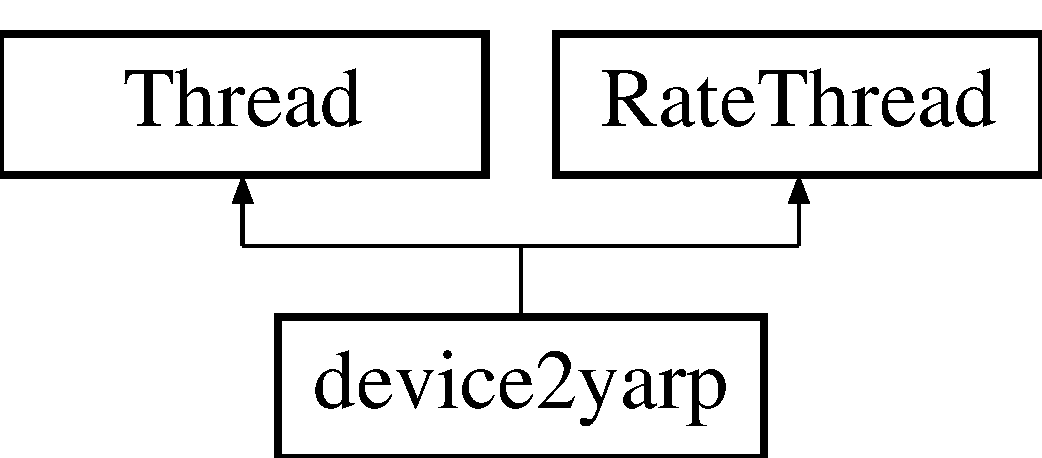
\includegraphics[height=2.000000cm]{classdevice2yarp}
\end{center}
\end{figure}
\subsection*{Public Member Functions}
\begin{DoxyCompactItemize}
\item 
{\bfseries device2yarp} (std\+::string device\+Number, bool save, std\+::string filename)\hypertarget{classdevice2yarp_a2871ae4aafa163197e3991486d3c8b18}{}\label{classdevice2yarp_a2871ae4aafa163197e3991486d3c8b18}

\item 
virtual void {\bfseries run} ()\hypertarget{classdevice2yarp_aa01eb91fc90a62cb29df3fdc8387cb54}{}\label{classdevice2yarp_aa01eb91fc90a62cb29df3fdc8387cb54}

\item 
virtual void {\bfseries thread\+Release} ()\hypertarget{classdevice2yarp_ae429ee3f9ab68ceea96daf63553e7700}{}\label{classdevice2yarp_ae429ee3f9ab68ceea96daf63553e7700}

\item 
void \hyperlink{classdevice2yarp_afbcd3cc36aeda39c389037ff480a0c3a}{prepare\+Biases} ()
\item 
void \hyperlink{classdevice2yarp_ab103ad6beed47415371ec71cc2ac30c3}{prepare\+Biases\+Right} ()
\item 
void \hyperlink{classdevice2yarp_aaaff6edb1a3d7830d6e87b14226e9207}{set\+Device\+Name} (std\+::string name)
\item 
void \hyperlink{classdevice2yarp_af60c47d12785c8bbc8ffb0a29f740a97}{close\+Device} ()
\item 
void \hyperlink{classdevice2yarp_a2ad1d6367e70bbc19d163b80a959843b}{prog\+Bias} (std\+::string name, int bits, int value, int camera=1)
\item 
void \hyperlink{classdevice2yarp_a148575c0588c481968e8e1c89aa1b2d8}{latch\+Commit} (int camera=1)
\item 
void \hyperlink{classdevice2yarp_ad5db8d09f97eb010e8037de3aafe4c0c}{latch\+Commit\+A\+Es} (int camera=1)
\item 
void \hyperlink{classdevice2yarp_a5227cd9f8f77fc3282abdb4f067c72db}{reset\+Pins} (int camera=1)
\item 
void \hyperlink{classdevice2yarp_acd91e6286807878481a293929579a358}{release\+Powerdown} (int camera=1)
\item 
void \hyperlink{classdevice2yarp_a468ec9658d04b2c89ea383a398245279}{set\+Powerdown} (int camera=1)
\item 
void \hyperlink{classdevice2yarp_a65726cde64ea739945753f5b51e84d8b}{prog\+Bit} (int bitvalue, int camera=1)
\item 
void \hyperlink{classdevice2yarp_a5291edc3d845bc6dd35c6d1a783ea80c}{prog\+Bit\+A\+Es} (int bitvalue, int camera=1)
\item 
void \hyperlink{classdevice2yarp_a39c03e4a4e0ac4b891947b872974f8af}{biasprogtx} (int time, int latch, int clock, int data, int powerdown=1, int camera=1)
\item 
void \hyperlink{classdevice2yarp_a19c60dd42e00da0e717da9fe17a5b2f5}{monitor} (int secs, int camera=1)
\item 
void \hyperlink{classdevice2yarp_a300aab882d64fa1a51b2058b530c8093}{sending\+Bias} ()
\item 
void \hyperlink{classdevice2yarp_a704565be367fa28840df912a97bdc25a}{set\+Only\+Left} ()
\item 
void \hyperlink{classdevice2yarp_a94653e9e8ce5ac4a60ae920f0ee41ee6}{set\+From\+Binary} (bool value)
\item 
void \hyperlink{classdevice2yarp_a1982c1021d9e51c789dfc5369dcb46bf}{set\+Binary\+File} (F\+I\+LE $\ast$f)
\item 
void \hyperlink{classdevice2yarp_a88ab89295bfefefbc9ac225dd5078dec}{set\+PR} (double value)
\item 
void \hyperlink{classdevice2yarp_a96f85845d4902b017e7d082cbc736735}{set\+F\+O\+LL} (double value)
\item 
void \hyperlink{classdevice2yarp_a813be66e7621e575682f44e92efa20ef}{set\+D\+I\+FF} (double value)
\item 
void \hyperlink{classdevice2yarp_ac072c8cf5341ae1bb187eacbaf8bc439}{set\+D\+I\+F\+F\+ON} (double value)
\item 
void \hyperlink{classdevice2yarp_a263fc557cd4333c9cff0e9e4a3f283cd}{set\+P\+UY} (double value)
\item 
void \hyperlink{classdevice2yarp_a24d972c0905025758a9d25607feaccf3}{set\+R\+E\+FR} (double value)
\item 
void \hyperlink{classdevice2yarp_add886f7ed984d3b47788df4cd294f2bc}{set\+R\+EQ} (double value)
\item 
void \hyperlink{classdevice2yarp_a202830f7c13eaff007c2594cc5e1d1ba}{set\+D\+I\+F\+F\+O\+FF} (double value)
\item 
void \hyperlink{classdevice2yarp_a1e9703e924441f50217aa4ded2be6c57}{set\+P\+UX} (double value)
\item 
void \hyperlink{classdevice2yarp_aea2c1f8287d1f9e95ac1ff2dc5ed878b}{set\+R\+E\+Q\+PD} (double value)
\item 
void \hyperlink{classdevice2yarp_afaf4e9eba2aa0d2f08602b7a03c6e5bf}{set\+I\+N\+J\+G\+ND} (double value)
\item 
void \hyperlink{classdevice2yarp_a469e0006636382fb25380147e146114f}{set\+C\+AS} (double value)
\item 
void \hyperlink{classdevice2yarp_a223f809aba867489a6b95c3b1ff66b15}{set\+P\+R\+Right} (double value)
\item 
void \hyperlink{classdevice2yarp_a27c6f1f15ceed7423118303431c9b54c}{set\+F\+O\+L\+L\+Right} (double value)
\item 
void \hyperlink{classdevice2yarp_add9e9df708995e75461d4589aae966c2}{set\+D\+I\+F\+F\+Right} (double value)
\item 
void \hyperlink{classdevice2yarp_aba1778322dffc46348dd78f0b86e56b0}{set\+D\+I\+F\+F\+O\+N\+Right} (double value)
\item 
void \hyperlink{classdevice2yarp_a0e60d43576b2d8f9c26519d09a14a564}{set\+P\+U\+Y\+Right} (double value)
\item 
void \hyperlink{classdevice2yarp_a026af71fd22a53e87896a1b1e5fbe2d9}{set\+R\+E\+F\+R\+Right} (double value)
\item 
void \hyperlink{classdevice2yarp_acb5c45d2835c3ea311f81daf2f4545cd}{set\+R\+E\+Q\+Right} (double value)
\item 
void \hyperlink{classdevice2yarp_a5a62082f903ae997ee15f3616c332635}{set\+D\+I\+F\+F\+O\+F\+F\+Right} (double value)
\item 
void \hyperlink{classdevice2yarp_a86ac1223c0a74dacebc26597e1a16ae9}{set\+P\+U\+X\+Right} (double value)
\item 
void \hyperlink{classdevice2yarp_aaac082c96f859df902389e60be83c328}{set\+R\+E\+Q\+P\+D\+Right} (double value)
\item 
void \hyperlink{classdevice2yarp_afab1c11e9c891a5b2103afa5d6101374}{set\+I\+N\+J\+G\+N\+D\+Right} (double value)
\item 
void \hyperlink{classdevice2yarp_aaa3573b8c4bb7e0348c97b87ef8edcd2}{set\+C\+A\+S\+Right} (double value)
\item 
void \hyperlink{classdevice2yarp_a4ef67bab52a9bbee2c590960afffc2e3}{set\+Dump\+Event} (bool value)
\item 
bool \hyperlink{classdevice2yarp_ac53bd1cc581717e681ad3ea0962db697}{set\+Dump\+File} (std\+::string value)
\item 
void \hyperlink{classdevice2yarp_ad5c9adf0e41f78d38a1d1b9265011dfa}{set\+Sync\+Bit} ()
\item 
double \hyperlink{classdevice2yarp_a85742caba0c13dbec757e034419ac570}{get\+PR} ()
\item 
double \hyperlink{classdevice2yarp_a45256821729711ac676b98fd86a2934b}{get\+F\+O\+LL} ()
\item 
double \hyperlink{classdevice2yarp_ac49ff696fd4ca634fb00188c7f84d5e0}{get\+D\+I\+FF} ()
\item 
double \hyperlink{classdevice2yarp_ae82c9cacfc6df370b144f764e1ba2d71}{get\+D\+I\+F\+F\+ON} ()
\item 
double \hyperlink{classdevice2yarp_a35e0c7313c78f7d4cfe7403b20742be7}{get\+P\+UY} ()
\item 
double \hyperlink{classdevice2yarp_a0cfbc83863780cb22777ea0df0dff4bb}{get\+R\+E\+FR} ()
\item 
double \hyperlink{classdevice2yarp_a02f8aaa21afea5a2c3cf690d4a7a810a}{get\+R\+EQ} ()
\item 
double \hyperlink{classdevice2yarp_aebb49f54bbbd1f89767ebc7473cf27f8}{get\+D\+I\+F\+F\+O\+FF} ()
\item 
double \hyperlink{classdevice2yarp_a17cabe5685326832b143a95bc079fce2}{get\+P\+UX} ()
\item 
double \hyperlink{classdevice2yarp_ad9668df280f370362a6be3d020766b53}{get\+R\+E\+Q\+PD} ()
\item 
double \hyperlink{classdevice2yarp_a71d866e65c1a1da500cde870fc9a4202}{get\+I\+N\+J\+G\+ND} ()
\item 
double \hyperlink{classdevice2yarp_a2695a28ec3a0864fd1f16bf58b757338}{get\+C\+AS} ()
\item 
bool {\bfseries initialise} (std\+::string module\+Name=\char`\"{}\char`\"{}, bool strict=false, bool check=false, std\+::string device\+Name=\char`\"{}\char`\"{}, unsigned int buffer\+Size=800000, unsigned int read\+Size=1024)\hypertarget{classdevice2yarp_ab94cdfb71b80d35005b43d42276266e1}{}\label{classdevice2yarp_ab94cdfb71b80d35005b43d42276266e1}

\item 
virtual void {\bfseries run} ()\hypertarget{classdevice2yarp_a2edb15ab91293f60b5ba2426ae247e1e}{}\label{classdevice2yarp_a2edb15ab91293f60b5ba2426ae247e1e}

\item 
virtual void {\bfseries thread\+Release} ()\hypertarget{classdevice2yarp_a684963ad891d4dc4e19c5128c88bfff0}{}\label{classdevice2yarp_a684963ad891d4dc4e19c5128c88bfff0}

\item 
virtual void {\bfseries after\+Start} (bool success)\hypertarget{classdevice2yarp_a1098424f146070180d0681787b771451}{}\label{classdevice2yarp_a1098424f146070180d0681787b771451}

\end{DoxyCompactItemize}


\subsection{Member Function Documentation}
\index{device2yarp@{device2yarp}!biasprogtx@{biasprogtx}}
\index{biasprogtx@{biasprogtx}!device2yarp@{device2yarp}}
\subsubsection[{\texorpdfstring{biasprogtx(int time, int latch, int clock, int data, int powerdown=1, int camera=1)}{biasprogtx(int time, int latch, int clock, int data, int powerdown=1, int camera=1)}}]{\setlength{\rightskip}{0pt plus 5cm}void device2yarp\+::biasprogtx (
\begin{DoxyParamCaption}
\item[{int}]{time, }
\item[{int}]{latch, }
\item[{int}]{clock, }
\item[{int}]{data, }
\item[{int}]{powerdown = {\ttfamily 1}, }
\item[{int}]{camera = {\ttfamily 1}}
\end{DoxyParamCaption}
)}\hypertarget{classdevice2yarp_a39c03e4a4e0ac4b891947b872974f8af}{}\label{classdevice2yarp_a39c03e4a4e0ac4b891947b872974f8af}
function that send biases to F\+P\+G\+A.\+The F\+P\+GA then first waits for the sequencer time to expire as for every other AE, then the lowest four bits of the AE, R\+I\+G\+H\+T/\+L\+E\+FT in 0x\+F\+F0000\+RL would be interpreted as new values for the bias programming pins. 
\begin{DoxyParams}{Parameters}
{\em time} & sequence time to expire before programming data \\
\hline
{\em latch} & control of the latch pin \\
\hline
{\em clock} & control of the clock \\
\hline
{\em data} & data that is sent \\
\hline
{\em powerdown} & control of the powerdown \\
\hline
{\em camera} & defines which camera is going to be programmed (Left 1, Right 0) \\
\hline
\end{DoxyParams}
\index{device2yarp@{device2yarp}!close\+Device@{close\+Device}}
\index{close\+Device@{close\+Device}!device2yarp@{device2yarp}}
\subsubsection[{\texorpdfstring{close\+Device()}{closeDevice()}}]{\setlength{\rightskip}{0pt plus 5cm}void device2yarp\+::close\+Device (
\begin{DoxyParamCaption}
{}
\end{DoxyParamCaption}
)}\hypertarget{classdevice2yarp_af60c47d12785c8bbc8ffb0a29f740a97}{}\label{classdevice2yarp_af60c47d12785c8bbc8ffb0a29f740a97}
function that correcly closes the device \index{device2yarp@{device2yarp}!get\+C\+AS@{get\+C\+AS}}
\index{get\+C\+AS@{get\+C\+AS}!device2yarp@{device2yarp}}
\subsubsection[{\texorpdfstring{get\+C\+A\+S()}{getCAS()}}]{\setlength{\rightskip}{0pt plus 5cm}double device2yarp\+::get\+C\+AS (
\begin{DoxyParamCaption}
{}
\end{DoxyParamCaption}
)\hspace{0.3cm}{\ttfamily [inline]}}\hypertarget{classdevice2yarp_a2695a28ec3a0864fd1f16bf58b757338}{}\label{classdevice2yarp_a2695a28ec3a0864fd1f16bf58b757338}
function that returns the bias for Left camera \begin{DoxyReturn}{Returns}
value of the bias 
\end{DoxyReturn}
\index{device2yarp@{device2yarp}!get\+D\+I\+FF@{get\+D\+I\+FF}}
\index{get\+D\+I\+FF@{get\+D\+I\+FF}!device2yarp@{device2yarp}}
\subsubsection[{\texorpdfstring{get\+D\+I\+F\+F()}{getDIFF()}}]{\setlength{\rightskip}{0pt plus 5cm}double device2yarp\+::get\+D\+I\+FF (
\begin{DoxyParamCaption}
{}
\end{DoxyParamCaption}
)\hspace{0.3cm}{\ttfamily [inline]}}\hypertarget{classdevice2yarp_ac49ff696fd4ca634fb00188c7f84d5e0}{}\label{classdevice2yarp_ac49ff696fd4ca634fb00188c7f84d5e0}
function that returns the bias for Left camera \begin{DoxyReturn}{Returns}
value of the bias 
\end{DoxyReturn}
\index{device2yarp@{device2yarp}!get\+D\+I\+F\+F\+O\+FF@{get\+D\+I\+F\+F\+O\+FF}}
\index{get\+D\+I\+F\+F\+O\+FF@{get\+D\+I\+F\+F\+O\+FF}!device2yarp@{device2yarp}}
\subsubsection[{\texorpdfstring{get\+D\+I\+F\+F\+O\+F\+F()}{getDIFFOFF()}}]{\setlength{\rightskip}{0pt plus 5cm}double device2yarp\+::get\+D\+I\+F\+F\+O\+FF (
\begin{DoxyParamCaption}
{}
\end{DoxyParamCaption}
)\hspace{0.3cm}{\ttfamily [inline]}}\hypertarget{classdevice2yarp_aebb49f54bbbd1f89767ebc7473cf27f8}{}\label{classdevice2yarp_aebb49f54bbbd1f89767ebc7473cf27f8}
function that returns the bias for Left camera \begin{DoxyReturn}{Returns}
value of the bias 
\end{DoxyReturn}
\index{device2yarp@{device2yarp}!get\+D\+I\+F\+F\+ON@{get\+D\+I\+F\+F\+ON}}
\index{get\+D\+I\+F\+F\+ON@{get\+D\+I\+F\+F\+ON}!device2yarp@{device2yarp}}
\subsubsection[{\texorpdfstring{get\+D\+I\+F\+F\+O\+N()}{getDIFFON()}}]{\setlength{\rightskip}{0pt plus 5cm}double device2yarp\+::get\+D\+I\+F\+F\+ON (
\begin{DoxyParamCaption}
{}
\end{DoxyParamCaption}
)\hspace{0.3cm}{\ttfamily [inline]}}\hypertarget{classdevice2yarp_ae82c9cacfc6df370b144f764e1ba2d71}{}\label{classdevice2yarp_ae82c9cacfc6df370b144f764e1ba2d71}
function that returns the bias for Left camera \begin{DoxyReturn}{Returns}
value of the bias 
\end{DoxyReturn}
\index{device2yarp@{device2yarp}!get\+F\+O\+LL@{get\+F\+O\+LL}}
\index{get\+F\+O\+LL@{get\+F\+O\+LL}!device2yarp@{device2yarp}}
\subsubsection[{\texorpdfstring{get\+F\+O\+L\+L()}{getFOLL()}}]{\setlength{\rightskip}{0pt plus 5cm}double device2yarp\+::get\+F\+O\+LL (
\begin{DoxyParamCaption}
{}
\end{DoxyParamCaption}
)\hspace{0.3cm}{\ttfamily [inline]}}\hypertarget{classdevice2yarp_a45256821729711ac676b98fd86a2934b}{}\label{classdevice2yarp_a45256821729711ac676b98fd86a2934b}
function that returns the bias for Left camera \begin{DoxyReturn}{Returns}
value of the bias 
\end{DoxyReturn}
\index{device2yarp@{device2yarp}!get\+I\+N\+J\+G\+ND@{get\+I\+N\+J\+G\+ND}}
\index{get\+I\+N\+J\+G\+ND@{get\+I\+N\+J\+G\+ND}!device2yarp@{device2yarp}}
\subsubsection[{\texorpdfstring{get\+I\+N\+J\+G\+N\+D()}{getINJGND()}}]{\setlength{\rightskip}{0pt plus 5cm}double device2yarp\+::get\+I\+N\+J\+G\+ND (
\begin{DoxyParamCaption}
{}
\end{DoxyParamCaption}
)\hspace{0.3cm}{\ttfamily [inline]}}\hypertarget{classdevice2yarp_a71d866e65c1a1da500cde870fc9a4202}{}\label{classdevice2yarp_a71d866e65c1a1da500cde870fc9a4202}
function that returns the bias for Left camera \begin{DoxyReturn}{Returns}
value of the bias 
\end{DoxyReturn}
\index{device2yarp@{device2yarp}!get\+PR@{get\+PR}}
\index{get\+PR@{get\+PR}!device2yarp@{device2yarp}}
\subsubsection[{\texorpdfstring{get\+P\+R()}{getPR()}}]{\setlength{\rightskip}{0pt plus 5cm}double device2yarp\+::get\+PR (
\begin{DoxyParamCaption}
{}
\end{DoxyParamCaption}
)\hspace{0.3cm}{\ttfamily [inline]}}\hypertarget{classdevice2yarp_a85742caba0c13dbec757e034419ac570}{}\label{classdevice2yarp_a85742caba0c13dbec757e034419ac570}
function that returns the bias for Left camera \begin{DoxyReturn}{Returns}
value of the bias 
\end{DoxyReturn}
\index{device2yarp@{device2yarp}!get\+P\+UX@{get\+P\+UX}}
\index{get\+P\+UX@{get\+P\+UX}!device2yarp@{device2yarp}}
\subsubsection[{\texorpdfstring{get\+P\+U\+X()}{getPUX()}}]{\setlength{\rightskip}{0pt plus 5cm}double device2yarp\+::get\+P\+UX (
\begin{DoxyParamCaption}
{}
\end{DoxyParamCaption}
)\hspace{0.3cm}{\ttfamily [inline]}}\hypertarget{classdevice2yarp_a17cabe5685326832b143a95bc079fce2}{}\label{classdevice2yarp_a17cabe5685326832b143a95bc079fce2}
function that returns the bias for Left camera \begin{DoxyReturn}{Returns}
value of the bias 
\end{DoxyReturn}
\index{device2yarp@{device2yarp}!get\+P\+UY@{get\+P\+UY}}
\index{get\+P\+UY@{get\+P\+UY}!device2yarp@{device2yarp}}
\subsubsection[{\texorpdfstring{get\+P\+U\+Y()}{getPUY()}}]{\setlength{\rightskip}{0pt plus 5cm}double device2yarp\+::get\+P\+UY (
\begin{DoxyParamCaption}
{}
\end{DoxyParamCaption}
)\hspace{0.3cm}{\ttfamily [inline]}}\hypertarget{classdevice2yarp_a35e0c7313c78f7d4cfe7403b20742be7}{}\label{classdevice2yarp_a35e0c7313c78f7d4cfe7403b20742be7}
function that returns the bias for Left camera \begin{DoxyReturn}{Returns}
value of the bias 
\end{DoxyReturn}
\index{device2yarp@{device2yarp}!get\+R\+E\+FR@{get\+R\+E\+FR}}
\index{get\+R\+E\+FR@{get\+R\+E\+FR}!device2yarp@{device2yarp}}
\subsubsection[{\texorpdfstring{get\+R\+E\+F\+R()}{getREFR()}}]{\setlength{\rightskip}{0pt plus 5cm}double device2yarp\+::get\+R\+E\+FR (
\begin{DoxyParamCaption}
{}
\end{DoxyParamCaption}
)\hspace{0.3cm}{\ttfamily [inline]}}\hypertarget{classdevice2yarp_a0cfbc83863780cb22777ea0df0dff4bb}{}\label{classdevice2yarp_a0cfbc83863780cb22777ea0df0dff4bb}
function that returns the bias for Left camera \begin{DoxyReturn}{Returns}
value of the bias 
\end{DoxyReturn}
\index{device2yarp@{device2yarp}!get\+R\+EQ@{get\+R\+EQ}}
\index{get\+R\+EQ@{get\+R\+EQ}!device2yarp@{device2yarp}}
\subsubsection[{\texorpdfstring{get\+R\+E\+Q()}{getREQ()}}]{\setlength{\rightskip}{0pt plus 5cm}double device2yarp\+::get\+R\+EQ (
\begin{DoxyParamCaption}
{}
\end{DoxyParamCaption}
)\hspace{0.3cm}{\ttfamily [inline]}}\hypertarget{classdevice2yarp_a02f8aaa21afea5a2c3cf690d4a7a810a}{}\label{classdevice2yarp_a02f8aaa21afea5a2c3cf690d4a7a810a}
function that returns the bias for Left camera \begin{DoxyReturn}{Returns}
value of the bias 
\end{DoxyReturn}
\index{device2yarp@{device2yarp}!get\+R\+E\+Q\+PD@{get\+R\+E\+Q\+PD}}
\index{get\+R\+E\+Q\+PD@{get\+R\+E\+Q\+PD}!device2yarp@{device2yarp}}
\subsubsection[{\texorpdfstring{get\+R\+E\+Q\+P\+D()}{getREQPD()}}]{\setlength{\rightskip}{0pt plus 5cm}double device2yarp\+::get\+R\+E\+Q\+PD (
\begin{DoxyParamCaption}
{}
\end{DoxyParamCaption}
)\hspace{0.3cm}{\ttfamily [inline]}}\hypertarget{classdevice2yarp_ad9668df280f370362a6be3d020766b53}{}\label{classdevice2yarp_ad9668df280f370362a6be3d020766b53}
function that returns the bias for Left camera \begin{DoxyReturn}{Returns}
value of the bias 
\end{DoxyReturn}
\index{device2yarp@{device2yarp}!latch\+Commit@{latch\+Commit}}
\index{latch\+Commit@{latch\+Commit}!device2yarp@{device2yarp}}
\subsubsection[{\texorpdfstring{latch\+Commit(int camera=1)}{latchCommit(int camera=1)}}]{\setlength{\rightskip}{0pt plus 5cm}void device2yarp\+::latch\+Commit (
\begin{DoxyParamCaption}
\item[{int}]{camera = {\ttfamily 1}}
\end{DoxyParamCaption}
)}\hypertarget{classdevice2yarp_a148575c0588c481968e8e1c89aa1b2d8}{}\label{classdevice2yarp_a148575c0588c481968e8e1c89aa1b2d8}
function used to append to a list of bits necessary to send the latch commit  reference to the camera (left 1, right 0) \index{device2yarp@{device2yarp}!latch\+Commit\+A\+Es@{latch\+Commit\+A\+Es}}
\index{latch\+Commit\+A\+Es@{latch\+Commit\+A\+Es}!device2yarp@{device2yarp}}
\subsubsection[{\texorpdfstring{latch\+Commit\+A\+Es(int camera=1)}{latchCommitAEs(int camera=1)}}]{\setlength{\rightskip}{0pt plus 5cm}void device2yarp\+::latch\+Commit\+A\+Es (
\begin{DoxyParamCaption}
\item[{int}]{camera = {\ttfamily 1}}
\end{DoxyParamCaption}
)}\hypertarget{classdevice2yarp_ad5db8d09f97eb010e8037de3aafe4c0c}{}\label{classdevice2yarp_ad5db8d09f97eb010e8037de3aafe4c0c}
function used to append to a list of bits necessary to send the latch commit (version 2)  reference to the camera (left 1, right 0) \index{device2yarp@{device2yarp}!monitor@{monitor}}
\index{monitor@{monitor}!device2yarp@{device2yarp}}
\subsubsection[{\texorpdfstring{monitor(int secs, int camera=1)}{monitor(int secs, int camera=1)}}]{\setlength{\rightskip}{0pt plus 5cm}void device2yarp\+::monitor (
\begin{DoxyParamCaption}
\item[{int}]{secs, }
\item[{int}]{camera = {\ttfamily 1}}
\end{DoxyParamCaption}
)}\hypertarget{classdevice2yarp_a19c60dd42e00da0e717da9fe17a5b2f5}{}\label{classdevice2yarp_a19c60dd42e00da0e717da9fe17a5b2f5}
function that monitors the output for seconds 
\begin{DoxyParams}{Parameters}
{\em secs} & number of seconds to wait  reference to the camera (left 1, right 0) \\
\hline
\end{DoxyParams}
\index{device2yarp@{device2yarp}!prepare\+Biases@{prepare\+Biases}}
\index{prepare\+Biases@{prepare\+Biases}!device2yarp@{device2yarp}}
\subsubsection[{\texorpdfstring{prepare\+Biases()}{prepareBiases()}}]{\setlength{\rightskip}{0pt plus 5cm}void device2yarp\+::prepare\+Biases (
\begin{DoxyParamCaption}
{}
\end{DoxyParamCaption}
)}\hypertarget{classdevice2yarp_afbcd3cc36aeda39c389037ff480a0c3a}{}\label{classdevice2yarp_afbcd3cc36aeda39c389037ff480a0c3a}
function that prepares biases either reading them from file or reading the default value \index{device2yarp@{device2yarp}!prepare\+Biases\+Right@{prepare\+Biases\+Right}}
\index{prepare\+Biases\+Right@{prepare\+Biases\+Right}!device2yarp@{device2yarp}}
\subsubsection[{\texorpdfstring{prepare\+Biases\+Right()}{prepareBiasesRight()}}]{\setlength{\rightskip}{0pt plus 5cm}void device2yarp\+::prepare\+Biases\+Right (
\begin{DoxyParamCaption}
{}
\end{DoxyParamCaption}
)}\hypertarget{classdevice2yarp_ab103ad6beed47415371ec71cc2ac30c3}{}\label{classdevice2yarp_ab103ad6beed47415371ec71cc2ac30c3}
function that prepares biases either reading them from file or reading the default value \index{device2yarp@{device2yarp}!prog\+Bias@{prog\+Bias}}
\index{prog\+Bias@{prog\+Bias}!device2yarp@{device2yarp}}
\subsubsection[{\texorpdfstring{prog\+Bias(std\+::string name, int bits, int value, int camera=1)}{progBias(std::string name, int bits, int value, int camera=1)}}]{\setlength{\rightskip}{0pt plus 5cm}void device2yarp\+::prog\+Bias (
\begin{DoxyParamCaption}
\item[{std\+::string}]{name, }
\item[{int}]{bits, }
\item[{int}]{value, }
\item[{int}]{camera = {\ttfamily 1}}
\end{DoxyParamCaption}
)}\hypertarget{classdevice2yarp_a2ad1d6367e70bbc19d163b80a959843b}{}\label{classdevice2yarp_a2ad1d6367e70bbc19d163b80a959843b}
function used to append to a list of commands every single bit necessary to program bias 
\begin{DoxyParams}{Parameters}
{\em name} & name of the bias to be set \\
\hline
{\em bits} & data of the programming \\
\hline
{\em value} & value of the programming  reference to the camera (left 1, right 0) \\
\hline
\end{DoxyParams}
\index{device2yarp@{device2yarp}!prog\+Bit@{prog\+Bit}}
\index{prog\+Bit@{prog\+Bit}!device2yarp@{device2yarp}}
\subsubsection[{\texorpdfstring{prog\+Bit(int bitvalue, int camera=1)}{progBit(int bitvalue, int camera=1)}}]{\setlength{\rightskip}{0pt plus 5cm}void device2yarp\+::prog\+Bit (
\begin{DoxyParamCaption}
\item[{int}]{bitvalue, }
\item[{int}]{camera = {\ttfamily 1}}
\end{DoxyParamCaption}
)}\hypertarget{classdevice2yarp_a65726cde64ea739945753f5b51e84d8b}{}\label{classdevice2yarp_a65726cde64ea739945753f5b51e84d8b}
correct sequence of signals necessary to program a bit 
\begin{DoxyParams}{Parameters}
{\em bitvalue} & value of the bit to be programmed  reference to the camera (left 1, right 0) \\
\hline
\end{DoxyParams}
\index{device2yarp@{device2yarp}!prog\+Bit\+A\+Es@{prog\+Bit\+A\+Es}}
\index{prog\+Bit\+A\+Es@{prog\+Bit\+A\+Es}!device2yarp@{device2yarp}}
\subsubsection[{\texorpdfstring{prog\+Bit\+A\+Es(int bitvalue, int camera=1)}{progBitAEs(int bitvalue, int camera=1)}}]{\setlength{\rightskip}{0pt plus 5cm}void device2yarp\+::prog\+Bit\+A\+Es (
\begin{DoxyParamCaption}
\item[{int}]{bitvalue, }
\item[{int}]{camera = {\ttfamily 1}}
\end{DoxyParamCaption}
)}\hypertarget{classdevice2yarp_a5291edc3d845bc6dd35c6d1a783ea80c}{}\label{classdevice2yarp_a5291edc3d845bc6dd35c6d1a783ea80c}
correct sequence of signals necessary to program a bit (version 2) 
\begin{DoxyParams}{Parameters}
{\em bitvalue} & value of the bit to be programmed  reference to the camera (left 1, right 0) \\
\hline
\end{DoxyParams}
\index{device2yarp@{device2yarp}!release\+Powerdown@{release\+Powerdown}}
\index{release\+Powerdown@{release\+Powerdown}!device2yarp@{device2yarp}}
\subsubsection[{\texorpdfstring{release\+Powerdown(int camera=1)}{releasePowerdown(int camera=1)}}]{\setlength{\rightskip}{0pt plus 5cm}void device2yarp\+::release\+Powerdown (
\begin{DoxyParamCaption}
\item[{int}]{camera = {\ttfamily 1}}
\end{DoxyParamCaption}
)}\hypertarget{classdevice2yarp_acd91e6286807878481a293929579a358}{}\label{classdevice2yarp_acd91e6286807878481a293929579a358}
function that sends the powerdown to the correct value after the biases have been programmed  reference to the camera (left 1, right 0) \index{device2yarp@{device2yarp}!reset\+Pins@{reset\+Pins}}
\index{reset\+Pins@{reset\+Pins}!device2yarp@{device2yarp}}
\subsubsection[{\texorpdfstring{reset\+Pins(int camera=1)}{resetPins(int camera=1)}}]{\setlength{\rightskip}{0pt plus 5cm}void device2yarp\+::reset\+Pins (
\begin{DoxyParamCaption}
\item[{int}]{camera = {\ttfamily 1}}
\end{DoxyParamCaption}
)}\hypertarget{classdevice2yarp_a5227cd9f8f77fc3282abdb4f067c72db}{}\label{classdevice2yarp_a5227cd9f8f77fc3282abdb4f067c72db}
function used to reset the device to default after a bias is sent  reference to the camera (left 1, right 0) \index{device2yarp@{device2yarp}!sending\+Bias@{sending\+Bias}}
\index{sending\+Bias@{sending\+Bias}!device2yarp@{device2yarp}}
\subsubsection[{\texorpdfstring{sending\+Bias()}{sendingBias()}}]{\setlength{\rightskip}{0pt plus 5cm}void device2yarp\+::sending\+Bias (
\begin{DoxyParamCaption}
{}
\end{DoxyParamCaption}
)}\hypertarget{classdevice2yarp_a300aab882d64fa1a51b2058b530c8093}{}\label{classdevice2yarp_a300aab882d64fa1a51b2058b530c8093}
fuction that connects to the device and write the sequence of signals to the device F\+P\+GA no matter what camera has been set the biases go to the board \index{device2yarp@{device2yarp}!set\+Binary\+File@{set\+Binary\+File}}
\index{set\+Binary\+File@{set\+Binary\+File}!device2yarp@{device2yarp}}
\subsubsection[{\texorpdfstring{set\+Binary\+File(\+F\+I\+L\+E $\ast$f)}{setBinaryFile(FILE *f)}}]{\setlength{\rightskip}{0pt plus 5cm}void device2yarp\+::set\+Binary\+File (
\begin{DoxyParamCaption}
\item[{F\+I\+LE $\ast$}]{f}
\end{DoxyParamCaption}
)\hspace{0.3cm}{\ttfamily [inline]}}\hypertarget{classdevice2yarp_a1982c1021d9e51c789dfc5369dcb46bf}{}\label{classdevice2yarp_a1982c1021d9e51c789dfc5369dcb46bf}
function that sets the reference of the input binary file 
\begin{DoxyParams}{Parameters}
{\em f} & pointer to the F\+I\+LE of the binary \\
\hline
\end{DoxyParams}
\index{device2yarp@{device2yarp}!set\+C\+AS@{set\+C\+AS}}
\index{set\+C\+AS@{set\+C\+AS}!device2yarp@{device2yarp}}
\subsubsection[{\texorpdfstring{set\+C\+A\+S(double value)}{setCAS(double value)}}]{\setlength{\rightskip}{0pt plus 5cm}void device2yarp\+::set\+C\+AS (
\begin{DoxyParamCaption}
\item[{double}]{value}
\end{DoxyParamCaption}
)\hspace{0.3cm}{\ttfamily [inline]}}\hypertarget{classdevice2yarp_a469e0006636382fb25380147e146114f}{}\label{classdevice2yarp_a469e0006636382fb25380147e146114f}
function that sets the bias 
\begin{DoxyParams}{Parameters}
{\em value} & value of the bias \\
\hline
\end{DoxyParams}
\index{device2yarp@{device2yarp}!set\+C\+A\+S\+Right@{set\+C\+A\+S\+Right}}
\index{set\+C\+A\+S\+Right@{set\+C\+A\+S\+Right}!device2yarp@{device2yarp}}
\subsubsection[{\texorpdfstring{set\+C\+A\+S\+Right(double value)}{setCASRight(double value)}}]{\setlength{\rightskip}{0pt plus 5cm}void device2yarp\+::set\+C\+A\+S\+Right (
\begin{DoxyParamCaption}
\item[{double}]{value}
\end{DoxyParamCaption}
)\hspace{0.3cm}{\ttfamily [inline]}}\hypertarget{classdevice2yarp_aaa3573b8c4bb7e0348c97b87ef8edcd2}{}\label{classdevice2yarp_aaa3573b8c4bb7e0348c97b87ef8edcd2}
function that sets the bias Right 
\begin{DoxyParams}{Parameters}
{\em value} & value of the bias \\
\hline
\end{DoxyParams}
\index{device2yarp@{device2yarp}!set\+Device\+Name@{set\+Device\+Name}}
\index{set\+Device\+Name@{set\+Device\+Name}!device2yarp@{device2yarp}}
\subsubsection[{\texorpdfstring{set\+Device\+Name(std\+::string name)}{setDeviceName(std::string name)}}]{\setlength{\rightskip}{0pt plus 5cm}void device2yarp\+::set\+Device\+Name (
\begin{DoxyParamCaption}
\item[{std\+::string}]{name}
\end{DoxyParamCaption}
)}\hypertarget{classdevice2yarp_aaaff6edb1a3d7830d6e87b14226e9207}{}\label{classdevice2yarp_aaaff6edb1a3d7830d6e87b14226e9207}
function used to set the name of the port device where biases are sent 
\begin{DoxyParams}{Parameters}
{\em name} & name of the port of the device \\
\hline
\end{DoxyParams}
\index{device2yarp@{device2yarp}!set\+D\+I\+FF@{set\+D\+I\+FF}}
\index{set\+D\+I\+FF@{set\+D\+I\+FF}!device2yarp@{device2yarp}}
\subsubsection[{\texorpdfstring{set\+D\+I\+F\+F(double value)}{setDIFF(double value)}}]{\setlength{\rightskip}{0pt plus 5cm}void device2yarp\+::set\+D\+I\+FF (
\begin{DoxyParamCaption}
\item[{double}]{value}
\end{DoxyParamCaption}
)\hspace{0.3cm}{\ttfamily [inline]}}\hypertarget{classdevice2yarp_a813be66e7621e575682f44e92efa20ef}{}\label{classdevice2yarp_a813be66e7621e575682f44e92efa20ef}
function that sets the bias 
\begin{DoxyParams}{Parameters}
{\em value} & value of the bias \\
\hline
\end{DoxyParams}
\index{device2yarp@{device2yarp}!set\+D\+I\+F\+F\+O\+FF@{set\+D\+I\+F\+F\+O\+FF}}
\index{set\+D\+I\+F\+F\+O\+FF@{set\+D\+I\+F\+F\+O\+FF}!device2yarp@{device2yarp}}
\subsubsection[{\texorpdfstring{set\+D\+I\+F\+F\+O\+F\+F(double value)}{setDIFFOFF(double value)}}]{\setlength{\rightskip}{0pt plus 5cm}void device2yarp\+::set\+D\+I\+F\+F\+O\+FF (
\begin{DoxyParamCaption}
\item[{double}]{value}
\end{DoxyParamCaption}
)\hspace{0.3cm}{\ttfamily [inline]}}\hypertarget{classdevice2yarp_a202830f7c13eaff007c2594cc5e1d1ba}{}\label{classdevice2yarp_a202830f7c13eaff007c2594cc5e1d1ba}
function that sets the bias 
\begin{DoxyParams}{Parameters}
{\em value} & value of the bias \\
\hline
\end{DoxyParams}
\index{device2yarp@{device2yarp}!set\+D\+I\+F\+F\+O\+F\+F\+Right@{set\+D\+I\+F\+F\+O\+F\+F\+Right}}
\index{set\+D\+I\+F\+F\+O\+F\+F\+Right@{set\+D\+I\+F\+F\+O\+F\+F\+Right}!device2yarp@{device2yarp}}
\subsubsection[{\texorpdfstring{set\+D\+I\+F\+F\+O\+F\+F\+Right(double value)}{setDIFFOFFRight(double value)}}]{\setlength{\rightskip}{0pt plus 5cm}void device2yarp\+::set\+D\+I\+F\+F\+O\+F\+F\+Right (
\begin{DoxyParamCaption}
\item[{double}]{value}
\end{DoxyParamCaption}
)\hspace{0.3cm}{\ttfamily [inline]}}\hypertarget{classdevice2yarp_a5a62082f903ae997ee15f3616c332635}{}\label{classdevice2yarp_a5a62082f903ae997ee15f3616c332635}
function that sets the bias Right 
\begin{DoxyParams}{Parameters}
{\em value} & value of the bias \\
\hline
\end{DoxyParams}
\index{device2yarp@{device2yarp}!set\+D\+I\+F\+F\+ON@{set\+D\+I\+F\+F\+ON}}
\index{set\+D\+I\+F\+F\+ON@{set\+D\+I\+F\+F\+ON}!device2yarp@{device2yarp}}
\subsubsection[{\texorpdfstring{set\+D\+I\+F\+F\+O\+N(double value)}{setDIFFON(double value)}}]{\setlength{\rightskip}{0pt plus 5cm}void device2yarp\+::set\+D\+I\+F\+F\+ON (
\begin{DoxyParamCaption}
\item[{double}]{value}
\end{DoxyParamCaption}
)\hspace{0.3cm}{\ttfamily [inline]}}\hypertarget{classdevice2yarp_ac072c8cf5341ae1bb187eacbaf8bc439}{}\label{classdevice2yarp_ac072c8cf5341ae1bb187eacbaf8bc439}
function that sets the bias 
\begin{DoxyParams}{Parameters}
{\em value} & value of the bias \\
\hline
\end{DoxyParams}
\index{device2yarp@{device2yarp}!set\+D\+I\+F\+F\+O\+N\+Right@{set\+D\+I\+F\+F\+O\+N\+Right}}
\index{set\+D\+I\+F\+F\+O\+N\+Right@{set\+D\+I\+F\+F\+O\+N\+Right}!device2yarp@{device2yarp}}
\subsubsection[{\texorpdfstring{set\+D\+I\+F\+F\+O\+N\+Right(double value)}{setDIFFONRight(double value)}}]{\setlength{\rightskip}{0pt plus 5cm}void device2yarp\+::set\+D\+I\+F\+F\+O\+N\+Right (
\begin{DoxyParamCaption}
\item[{double}]{value}
\end{DoxyParamCaption}
)\hspace{0.3cm}{\ttfamily [inline]}}\hypertarget{classdevice2yarp_aba1778322dffc46348dd78f0b86e56b0}{}\label{classdevice2yarp_aba1778322dffc46348dd78f0b86e56b0}
function that sets the bias Right 
\begin{DoxyParams}{Parameters}
{\em value} & value of the bias \\
\hline
\end{DoxyParams}
\index{device2yarp@{device2yarp}!set\+D\+I\+F\+F\+Right@{set\+D\+I\+F\+F\+Right}}
\index{set\+D\+I\+F\+F\+Right@{set\+D\+I\+F\+F\+Right}!device2yarp@{device2yarp}}
\subsubsection[{\texorpdfstring{set\+D\+I\+F\+F\+Right(double value)}{setDIFFRight(double value)}}]{\setlength{\rightskip}{0pt plus 5cm}void device2yarp\+::set\+D\+I\+F\+F\+Right (
\begin{DoxyParamCaption}
\item[{double}]{value}
\end{DoxyParamCaption}
)\hspace{0.3cm}{\ttfamily [inline]}}\hypertarget{classdevice2yarp_add9e9df708995e75461d4589aae966c2}{}\label{classdevice2yarp_add9e9df708995e75461d4589aae966c2}
function that sets the bias Right 
\begin{DoxyParams}{Parameters}
{\em value} & value of the bias \\
\hline
\end{DoxyParams}
\index{device2yarp@{device2yarp}!set\+Dump\+Event@{set\+Dump\+Event}}
\index{set\+Dump\+Event@{set\+Dump\+Event}!device2yarp@{device2yarp}}
\subsubsection[{\texorpdfstring{set\+Dump\+Event(bool value)}{setDumpEvent(bool value)}}]{\setlength{\rightskip}{0pt plus 5cm}void device2yarp\+::set\+Dump\+Event (
\begin{DoxyParamCaption}
\item[{bool}]{value}
\end{DoxyParamCaption}
)}\hypertarget{classdevice2yarp_a4ef67bab52a9bbee2c590960afffc2e3}{}\label{classdevice2yarp_a4ef67bab52a9bbee2c590960afffc2e3}
indicates whether the event has to be saved in a file \index{device2yarp@{device2yarp}!set\+Dump\+File@{set\+Dump\+File}}
\index{set\+Dump\+File@{set\+Dump\+File}!device2yarp@{device2yarp}}
\subsubsection[{\texorpdfstring{set\+Dump\+File(std\+::string value)}{setDumpFile(std::string value)}}]{\setlength{\rightskip}{0pt plus 5cm}bool device2yarp\+::set\+Dump\+File (
\begin{DoxyParamCaption}
\item[{std\+::string}]{value}
\end{DoxyParamCaption}
)}\hypertarget{classdevice2yarp_ac53bd1cc581717e681ad3ea0962db697}{}\label{classdevice2yarp_ac53bd1cc581717e681ad3ea0962db697}
reference to the name of the file where events are dumped \index{device2yarp@{device2yarp}!set\+F\+O\+LL@{set\+F\+O\+LL}}
\index{set\+F\+O\+LL@{set\+F\+O\+LL}!device2yarp@{device2yarp}}
\subsubsection[{\texorpdfstring{set\+F\+O\+L\+L(double value)}{setFOLL(double value)}}]{\setlength{\rightskip}{0pt plus 5cm}void device2yarp\+::set\+F\+O\+LL (
\begin{DoxyParamCaption}
\item[{double}]{value}
\end{DoxyParamCaption}
)\hspace{0.3cm}{\ttfamily [inline]}}\hypertarget{classdevice2yarp_a96f85845d4902b017e7d082cbc736735}{}\label{classdevice2yarp_a96f85845d4902b017e7d082cbc736735}
function that sets the bias 
\begin{DoxyParams}{Parameters}
{\em value} & value of the bias \\
\hline
\end{DoxyParams}
\index{device2yarp@{device2yarp}!set\+F\+O\+L\+L\+Right@{set\+F\+O\+L\+L\+Right}}
\index{set\+F\+O\+L\+L\+Right@{set\+F\+O\+L\+L\+Right}!device2yarp@{device2yarp}}
\subsubsection[{\texorpdfstring{set\+F\+O\+L\+L\+Right(double value)}{setFOLLRight(double value)}}]{\setlength{\rightskip}{0pt plus 5cm}void device2yarp\+::set\+F\+O\+L\+L\+Right (
\begin{DoxyParamCaption}
\item[{double}]{value}
\end{DoxyParamCaption}
)\hspace{0.3cm}{\ttfamily [inline]}}\hypertarget{classdevice2yarp_a27c6f1f15ceed7423118303431c9b54c}{}\label{classdevice2yarp_a27c6f1f15ceed7423118303431c9b54c}
function that sets the bias Right 
\begin{DoxyParams}{Parameters}
{\em value} & value of the bias \\
\hline
\end{DoxyParams}
\index{device2yarp@{device2yarp}!set\+From\+Binary@{set\+From\+Binary}}
\index{set\+From\+Binary@{set\+From\+Binary}!device2yarp@{device2yarp}}
\subsubsection[{\texorpdfstring{set\+From\+Binary(bool value)}{setFromBinary(bool value)}}]{\setlength{\rightskip}{0pt plus 5cm}void device2yarp\+::set\+From\+Binary (
\begin{DoxyParamCaption}
\item[{bool}]{value}
\end{DoxyParamCaption}
)\hspace{0.3cm}{\ttfamily [inline]}}\hypertarget{classdevice2yarp_a94653e9e8ce5ac4a60ae920f0ee41ee6}{}\label{classdevice2yarp_a94653e9e8ce5ac4a60ae920f0ee41ee6}
set the flag that regulates whether the biases are read from binary or copied from default values \index{device2yarp@{device2yarp}!set\+I\+N\+J\+G\+ND@{set\+I\+N\+J\+G\+ND}}
\index{set\+I\+N\+J\+G\+ND@{set\+I\+N\+J\+G\+ND}!device2yarp@{device2yarp}}
\subsubsection[{\texorpdfstring{set\+I\+N\+J\+G\+N\+D(double value)}{setINJGND(double value)}}]{\setlength{\rightskip}{0pt plus 5cm}void device2yarp\+::set\+I\+N\+J\+G\+ND (
\begin{DoxyParamCaption}
\item[{double}]{value}
\end{DoxyParamCaption}
)\hspace{0.3cm}{\ttfamily [inline]}}\hypertarget{classdevice2yarp_afaf4e9eba2aa0d2f08602b7a03c6e5bf}{}\label{classdevice2yarp_afaf4e9eba2aa0d2f08602b7a03c6e5bf}
function that sets the bias 
\begin{DoxyParams}{Parameters}
{\em value} & value of the bias \\
\hline
\end{DoxyParams}
\index{device2yarp@{device2yarp}!set\+I\+N\+J\+G\+N\+D\+Right@{set\+I\+N\+J\+G\+N\+D\+Right}}
\index{set\+I\+N\+J\+G\+N\+D\+Right@{set\+I\+N\+J\+G\+N\+D\+Right}!device2yarp@{device2yarp}}
\subsubsection[{\texorpdfstring{set\+I\+N\+J\+G\+N\+D\+Right(double value)}{setINJGNDRight(double value)}}]{\setlength{\rightskip}{0pt plus 5cm}void device2yarp\+::set\+I\+N\+J\+G\+N\+D\+Right (
\begin{DoxyParamCaption}
\item[{double}]{value}
\end{DoxyParamCaption}
)\hspace{0.3cm}{\ttfamily [inline]}}\hypertarget{classdevice2yarp_afab1c11e9c891a5b2103afa5d6101374}{}\label{classdevice2yarp_afab1c11e9c891a5b2103afa5d6101374}
function that sets the bias Right 
\begin{DoxyParams}{Parameters}
{\em value} & value of the bias \\
\hline
\end{DoxyParams}
\index{device2yarp@{device2yarp}!set\+Only\+Left@{set\+Only\+Left}}
\index{set\+Only\+Left@{set\+Only\+Left}!device2yarp@{device2yarp}}
\subsubsection[{\texorpdfstring{set\+Only\+Left()}{setOnlyLeft()}}]{\setlength{\rightskip}{0pt plus 5cm}void device2yarp\+::set\+Only\+Left (
\begin{DoxyParamCaption}
{}
\end{DoxyParamCaption}
)\hspace{0.3cm}{\ttfamily [inline]}}\hypertarget{classdevice2yarp_a704565be367fa28840df912a97bdc25a}{}\label{classdevice2yarp_a704565be367fa28840df912a97bdc25a}
function that switches only the left camera ON \index{device2yarp@{device2yarp}!set\+Powerdown@{set\+Powerdown}}
\index{set\+Powerdown@{set\+Powerdown}!device2yarp@{device2yarp}}
\subsubsection[{\texorpdfstring{set\+Powerdown(int camera=1)}{setPowerdown(int camera=1)}}]{\setlength{\rightskip}{0pt plus 5cm}void device2yarp\+::set\+Powerdown (
\begin{DoxyParamCaption}
\item[{int}]{camera = {\ttfamily 1}}
\end{DoxyParamCaption}
)}\hypertarget{classdevice2yarp_a468ec9658d04b2c89ea383a398245279}{}\label{classdevice2yarp_a468ec9658d04b2c89ea383a398245279}
function that sends the powerdown to the correct value before switching the device off  reference to the camera (left 1, right 0) \index{device2yarp@{device2yarp}!set\+PR@{set\+PR}}
\index{set\+PR@{set\+PR}!device2yarp@{device2yarp}}
\subsubsection[{\texorpdfstring{set\+P\+R(double value)}{setPR(double value)}}]{\setlength{\rightskip}{0pt plus 5cm}void device2yarp\+::set\+PR (
\begin{DoxyParamCaption}
\item[{double}]{value}
\end{DoxyParamCaption}
)\hspace{0.3cm}{\ttfamily [inline]}}\hypertarget{classdevice2yarp_a88ab89295bfefefbc9ac225dd5078dec}{}\label{classdevice2yarp_a88ab89295bfefefbc9ac225dd5078dec}
function that sets the bias 
\begin{DoxyParams}{Parameters}
{\em value} & value of the bias \\
\hline
\end{DoxyParams}
\index{device2yarp@{device2yarp}!set\+P\+R\+Right@{set\+P\+R\+Right}}
\index{set\+P\+R\+Right@{set\+P\+R\+Right}!device2yarp@{device2yarp}}
\subsubsection[{\texorpdfstring{set\+P\+R\+Right(double value)}{setPRRight(double value)}}]{\setlength{\rightskip}{0pt plus 5cm}void device2yarp\+::set\+P\+R\+Right (
\begin{DoxyParamCaption}
\item[{double}]{value}
\end{DoxyParamCaption}
)\hspace{0.3cm}{\ttfamily [inline]}}\hypertarget{classdevice2yarp_a223f809aba867489a6b95c3b1ff66b15}{}\label{classdevice2yarp_a223f809aba867489a6b95c3b1ff66b15}
function that sets the bias Right 
\begin{DoxyParams}{Parameters}
{\em value} & value of the bias \\
\hline
\end{DoxyParams}
\index{device2yarp@{device2yarp}!set\+P\+UX@{set\+P\+UX}}
\index{set\+P\+UX@{set\+P\+UX}!device2yarp@{device2yarp}}
\subsubsection[{\texorpdfstring{set\+P\+U\+X(double value)}{setPUX(double value)}}]{\setlength{\rightskip}{0pt plus 5cm}void device2yarp\+::set\+P\+UX (
\begin{DoxyParamCaption}
\item[{double}]{value}
\end{DoxyParamCaption}
)\hspace{0.3cm}{\ttfamily [inline]}}\hypertarget{classdevice2yarp_a1e9703e924441f50217aa4ded2be6c57}{}\label{classdevice2yarp_a1e9703e924441f50217aa4ded2be6c57}
function that sets the bias 
\begin{DoxyParams}{Parameters}
{\em value} & value of the bias \\
\hline
\end{DoxyParams}
\index{device2yarp@{device2yarp}!set\+P\+U\+X\+Right@{set\+P\+U\+X\+Right}}
\index{set\+P\+U\+X\+Right@{set\+P\+U\+X\+Right}!device2yarp@{device2yarp}}
\subsubsection[{\texorpdfstring{set\+P\+U\+X\+Right(double value)}{setPUXRight(double value)}}]{\setlength{\rightskip}{0pt plus 5cm}void device2yarp\+::set\+P\+U\+X\+Right (
\begin{DoxyParamCaption}
\item[{double}]{value}
\end{DoxyParamCaption}
)\hspace{0.3cm}{\ttfamily [inline]}}\hypertarget{classdevice2yarp_a86ac1223c0a74dacebc26597e1a16ae9}{}\label{classdevice2yarp_a86ac1223c0a74dacebc26597e1a16ae9}
function that sets the bias Right 
\begin{DoxyParams}{Parameters}
{\em value} & value of the bias \\
\hline
\end{DoxyParams}
\index{device2yarp@{device2yarp}!set\+P\+UY@{set\+P\+UY}}
\index{set\+P\+UY@{set\+P\+UY}!device2yarp@{device2yarp}}
\subsubsection[{\texorpdfstring{set\+P\+U\+Y(double value)}{setPUY(double value)}}]{\setlength{\rightskip}{0pt plus 5cm}void device2yarp\+::set\+P\+UY (
\begin{DoxyParamCaption}
\item[{double}]{value}
\end{DoxyParamCaption}
)\hspace{0.3cm}{\ttfamily [inline]}}\hypertarget{classdevice2yarp_a263fc557cd4333c9cff0e9e4a3f283cd}{}\label{classdevice2yarp_a263fc557cd4333c9cff0e9e4a3f283cd}
function that sets the bias 
\begin{DoxyParams}{Parameters}
{\em value} & value of the bias \\
\hline
\end{DoxyParams}
\index{device2yarp@{device2yarp}!set\+P\+U\+Y\+Right@{set\+P\+U\+Y\+Right}}
\index{set\+P\+U\+Y\+Right@{set\+P\+U\+Y\+Right}!device2yarp@{device2yarp}}
\subsubsection[{\texorpdfstring{set\+P\+U\+Y\+Right(double value)}{setPUYRight(double value)}}]{\setlength{\rightskip}{0pt plus 5cm}void device2yarp\+::set\+P\+U\+Y\+Right (
\begin{DoxyParamCaption}
\item[{double}]{value}
\end{DoxyParamCaption}
)\hspace{0.3cm}{\ttfamily [inline]}}\hypertarget{classdevice2yarp_a0e60d43576b2d8f9c26519d09a14a564}{}\label{classdevice2yarp_a0e60d43576b2d8f9c26519d09a14a564}
function that sets the bias Right 
\begin{DoxyParams}{Parameters}
{\em value} & value of the bias \\
\hline
\end{DoxyParams}
\index{device2yarp@{device2yarp}!set\+R\+E\+FR@{set\+R\+E\+FR}}
\index{set\+R\+E\+FR@{set\+R\+E\+FR}!device2yarp@{device2yarp}}
\subsubsection[{\texorpdfstring{set\+R\+E\+F\+R(double value)}{setREFR(double value)}}]{\setlength{\rightskip}{0pt plus 5cm}void device2yarp\+::set\+R\+E\+FR (
\begin{DoxyParamCaption}
\item[{double}]{value}
\end{DoxyParamCaption}
)\hspace{0.3cm}{\ttfamily [inline]}}\hypertarget{classdevice2yarp_a24d972c0905025758a9d25607feaccf3}{}\label{classdevice2yarp_a24d972c0905025758a9d25607feaccf3}
function that sets the bias 
\begin{DoxyParams}{Parameters}
{\em value} & value of the bias \\
\hline
\end{DoxyParams}
\index{device2yarp@{device2yarp}!set\+R\+E\+F\+R\+Right@{set\+R\+E\+F\+R\+Right}}
\index{set\+R\+E\+F\+R\+Right@{set\+R\+E\+F\+R\+Right}!device2yarp@{device2yarp}}
\subsubsection[{\texorpdfstring{set\+R\+E\+F\+R\+Right(double value)}{setREFRRight(double value)}}]{\setlength{\rightskip}{0pt plus 5cm}void device2yarp\+::set\+R\+E\+F\+R\+Right (
\begin{DoxyParamCaption}
\item[{double}]{value}
\end{DoxyParamCaption}
)\hspace{0.3cm}{\ttfamily [inline]}}\hypertarget{classdevice2yarp_a026af71fd22a53e87896a1b1e5fbe2d9}{}\label{classdevice2yarp_a026af71fd22a53e87896a1b1e5fbe2d9}
function that sets the bias Right 
\begin{DoxyParams}{Parameters}
{\em value} & value of the bias \\
\hline
\end{DoxyParams}
\index{device2yarp@{device2yarp}!set\+R\+EQ@{set\+R\+EQ}}
\index{set\+R\+EQ@{set\+R\+EQ}!device2yarp@{device2yarp}}
\subsubsection[{\texorpdfstring{set\+R\+E\+Q(double value)}{setREQ(double value)}}]{\setlength{\rightskip}{0pt plus 5cm}void device2yarp\+::set\+R\+EQ (
\begin{DoxyParamCaption}
\item[{double}]{value}
\end{DoxyParamCaption}
)\hspace{0.3cm}{\ttfamily [inline]}}\hypertarget{classdevice2yarp_add886f7ed984d3b47788df4cd294f2bc}{}\label{classdevice2yarp_add886f7ed984d3b47788df4cd294f2bc}
function that sets the bias 
\begin{DoxyParams}{Parameters}
{\em value} & value of the bias \\
\hline
\end{DoxyParams}
\index{device2yarp@{device2yarp}!set\+R\+E\+Q\+PD@{set\+R\+E\+Q\+PD}}
\index{set\+R\+E\+Q\+PD@{set\+R\+E\+Q\+PD}!device2yarp@{device2yarp}}
\subsubsection[{\texorpdfstring{set\+R\+E\+Q\+P\+D(double value)}{setREQPD(double value)}}]{\setlength{\rightskip}{0pt plus 5cm}void device2yarp\+::set\+R\+E\+Q\+PD (
\begin{DoxyParamCaption}
\item[{double}]{value}
\end{DoxyParamCaption}
)\hspace{0.3cm}{\ttfamily [inline]}}\hypertarget{classdevice2yarp_aea2c1f8287d1f9e95ac1ff2dc5ed878b}{}\label{classdevice2yarp_aea2c1f8287d1f9e95ac1ff2dc5ed878b}
function that sets the bias 
\begin{DoxyParams}{Parameters}
{\em value} & value of the bias \\
\hline
\end{DoxyParams}
\index{device2yarp@{device2yarp}!set\+R\+E\+Q\+P\+D\+Right@{set\+R\+E\+Q\+P\+D\+Right}}
\index{set\+R\+E\+Q\+P\+D\+Right@{set\+R\+E\+Q\+P\+D\+Right}!device2yarp@{device2yarp}}
\subsubsection[{\texorpdfstring{set\+R\+E\+Q\+P\+D\+Right(double value)}{setREQPDRight(double value)}}]{\setlength{\rightskip}{0pt plus 5cm}void device2yarp\+::set\+R\+E\+Q\+P\+D\+Right (
\begin{DoxyParamCaption}
\item[{double}]{value}
\end{DoxyParamCaption}
)\hspace{0.3cm}{\ttfamily [inline]}}\hypertarget{classdevice2yarp_aaac082c96f859df902389e60be83c328}{}\label{classdevice2yarp_aaac082c96f859df902389e60be83c328}
function that sets the bias Right 
\begin{DoxyParams}{Parameters}
{\em value} & value of the bias \\
\hline
\end{DoxyParams}
\index{device2yarp@{device2yarp}!set\+R\+E\+Q\+Right@{set\+R\+E\+Q\+Right}}
\index{set\+R\+E\+Q\+Right@{set\+R\+E\+Q\+Right}!device2yarp@{device2yarp}}
\subsubsection[{\texorpdfstring{set\+R\+E\+Q\+Right(double value)}{setREQRight(double value)}}]{\setlength{\rightskip}{0pt plus 5cm}void device2yarp\+::set\+R\+E\+Q\+Right (
\begin{DoxyParamCaption}
\item[{double}]{value}
\end{DoxyParamCaption}
)\hspace{0.3cm}{\ttfamily [inline]}}\hypertarget{classdevice2yarp_acb5c45d2835c3ea311f81daf2f4545cd}{}\label{classdevice2yarp_acb5c45d2835c3ea311f81daf2f4545cd}
function that sets the bias Right 
\begin{DoxyParams}{Parameters}
{\em value} & value of the bias \\
\hline
\end{DoxyParams}
\index{device2yarp@{device2yarp}!set\+Sync\+Bit@{set\+Sync\+Bit}}
\index{set\+Sync\+Bit@{set\+Sync\+Bit}!device2yarp@{device2yarp}}
\subsubsection[{\texorpdfstring{set\+Sync\+Bit()}{setSyncBit()}}]{\setlength{\rightskip}{0pt plus 5cm}void device2yarp\+::set\+Sync\+Bit (
\begin{DoxyParamCaption}
{}
\end{DoxyParamCaption}
)}\hypertarget{classdevice2yarp_ad5c9adf0e41f78d38a1d1b9265011dfa}{}\label{classdevice2yarp_ad5c9adf0e41f78d38a1d1b9265011dfa}
add a bit to the adress to synchronize several records 

The documentation for this class was generated from the following files\+:\begin{DoxyCompactItemize}
\item 
/home/aglover/workspace/projects/event-\/driven/src/hardwareio/aex\+Grabber/include/\hyperlink{device2yarp_8h}{device2yarp.\+h}\item 
/home/aglover/workspace/projects/event-\/driven/src/hardwareio/zynq\+Grabber/include/yarp\+Interface.\+h\item 
/home/aglover/workspace/projects/event-\/driven/src/hardwareio/aex\+Grabber/src/device2yarp.\+cpp\item 
/home/aglover/workspace/projects/event-\/driven/src/hardwareio/zynq\+Grabber/src/yarp\+Interface.\+cpp\end{DoxyCompactItemize}

\hypertarget{classEventBottleManager}{}\section{Event\+Bottle\+Manager Class Reference}
\label{classEventBottleManager}\index{Event\+Bottle\+Manager@{Event\+Bottle\+Manager}}
Inheritance diagram for Event\+Bottle\+Manager\+:\begin{figure}[H]
\begin{center}
\leavevmode
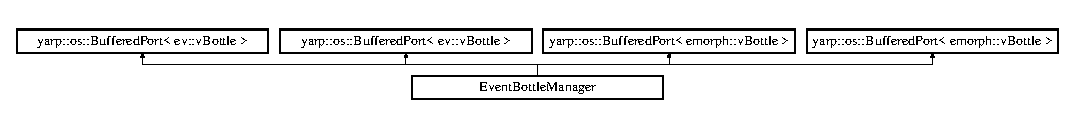
\includegraphics[height=1.106719cm]{classEventBottleManager}
\end{center}
\end{figure}
\subsection*{Public Member Functions}
\begin{DoxyCompactItemize}
\item 
bool {\bfseries open} (const std\+::string \&name)\hypertarget{classEventBottleManager_a41ce7bd0a716ab0a88c1ad505b02d20b}{}\label{classEventBottleManager_a41ce7bd0a716ab0a88c1ad505b02d20b}

\item 
void {\bfseries close} ()\hypertarget{classEventBottleManager_aa155dc6f20728e9f7ff13abf720ea6b8}{}\label{classEventBottleManager_aa155dc6f20728e9f7ff13abf720ea6b8}

\item 
void {\bfseries interrupt} ()\hypertarget{classEventBottleManager_a15152f9daa40714334c2da3871f959a9}{}\label{classEventBottleManager_a15152f9daa40714334c2da3871f959a9}

\item 
void {\bfseries on\+Read} (emorph\+::v\+Bottle \&bot)\hypertarget{classEventBottleManager_a9571d64d4640ef5a38f03a286d27425e}{}\label{classEventBottleManager_a9571d64d4640ef5a38f03a286d27425e}

\item 
bool {\bfseries open} (const std\+::string \&name)\hypertarget{classEventBottleManager_a41ce7bd0a716ab0a88c1ad505b02d20b}{}\label{classEventBottleManager_a41ce7bd0a716ab0a88c1ad505b02d20b}

\item 
void {\bfseries close} ()\hypertarget{classEventBottleManager_aa155dc6f20728e9f7ff13abf720ea6b8}{}\label{classEventBottleManager_aa155dc6f20728e9f7ff13abf720ea6b8}

\item 
void {\bfseries interrupt} ()\hypertarget{classEventBottleManager_a15152f9daa40714334c2da3871f959a9}{}\label{classEventBottleManager_a15152f9daa40714334c2da3871f959a9}

\item 
void {\bfseries on\+Read} (emorph\+::v\+Bottle \&bot)\hypertarget{classEventBottleManager_a9571d64d4640ef5a38f03a286d27425e}{}\label{classEventBottleManager_a9571d64d4640ef5a38f03a286d27425e}

\item 
void {\bfseries set\+All\+Parameters} (double alpha\+\_\+shape, double alpha\+\_\+pos, double Tact, double Tinact, double Tfree, double Tevent, double SigX, double SigY, double Sig\+XY, bool Fixedshape, int Regrate, double Maxdist, double decay\+\_\+tau, double cluster\+Limit)\hypertarget{classEventBottleManager_a451485cebdadbbad730d176894d9f0b1}{}\label{classEventBottleManager_a451485cebdadbbad730d176894d9f0b1}

\item 
bool {\bfseries open} (std\+::string module\+Name)\hypertarget{classEventBottleManager_a82d3237530dcc455f3ceae4e1db4f6df}{}\label{classEventBottleManager_a82d3237530dcc455f3ceae4e1db4f6df}

\item 
bool {\bfseries init} ()\hypertarget{classEventBottleManager_af4d71177a30fdd8fc40485b91abdae10}{}\label{classEventBottleManager_af4d71177a30fdd8fc40485b91abdae10}

\item 
void {\bfseries close} ()\hypertarget{classEventBottleManager_aa155dc6f20728e9f7ff13abf720ea6b8}{}\label{classEventBottleManager_aa155dc6f20728e9f7ff13abf720ea6b8}

\item 
void {\bfseries on\+Read} (\hyperlink{classev_1_1vBottle}{ev\+::v\+Bottle} \&bot)\hypertarget{classEventBottleManager_aa848144d06e1970fb3c0482da838f078}{}\label{classEventBottleManager_aa848144d06e1970fb3c0482da838f078}

\item 
void {\bfseries interrupt} ()\hypertarget{classEventBottleManager_a15152f9daa40714334c2da3871f959a9}{}\label{classEventBottleManager_a15152f9daa40714334c2da3871f959a9}

\item 
bool {\bfseries open} (const std\+::string \&name)\hypertarget{classEventBottleManager_a41ce7bd0a716ab0a88c1ad505b02d20b}{}\label{classEventBottleManager_a41ce7bd0a716ab0a88c1ad505b02d20b}

\item 
void {\bfseries on\+Read} (\hyperlink{classev_1_1vBottle}{ev\+::v\+Bottle} \&bot)\hypertarget{classEventBottleManager_aa848144d06e1970fb3c0482da838f078}{}\label{classEventBottleManager_aa848144d06e1970fb3c0482da838f078}

\item 
unsigned long int {\bfseries get\+Time} ()\hypertarget{classEventBottleManager_af15b5cfdc457500423111c22dee264d2}{}\label{classEventBottleManager_af15b5cfdc457500423111c22dee264d2}

\item 
unsigned long int {\bfseries pop\+Count} ()\hypertarget{classEventBottleManager_a0b4fd036f14e713194d079467021ba3b}{}\label{classEventBottleManager_a0b4fd036f14e713194d079467021ba3b}

\end{DoxyCompactItemize}


The documentation for this class was generated from the following files\+:\begin{DoxyCompactItemize}
\item 
/home/aglover/workspace/projects/event-\/driven/src/modules/spinconverter/include/spinconverter.\+h\item 
/home/aglover/workspace/projects/event-\/driven/src/modules/template/include/v\+Template.\+h\item 
/home/aglover/workspace/projects/event-\/driven/src/modules/v\+Cluster/include/event\+Clustering.\+h\item 
/home/aglover/workspace/projects/event-\/driven/src/robotio/autosaccade/include/auto\+Saccade.\+h\item 
/home/aglover/workspace/projects/event-\/driven/src/modules/spinconverter/src/spinconverter.\+cpp\item 
/home/aglover/workspace/projects/event-\/driven/src/modules/template/src/v\+Template.\+cpp\item 
/home/aglover/workspace/projects/event-\/driven/src/modules/v\+Cluster/src/event\+Clustering.\+cpp\item 
/home/aglover/workspace/projects/event-\/driven/src/robotio/autosaccade/src/auto\+Saccade.\+cpp\end{DoxyCompactItemize}

\hypertarget{classEventClustering}{}\section{Event\+Clustering Class Reference}
\label{classEventClustering}\index{Event\+Clustering@{Event\+Clustering}}
Inheritance diagram for Event\+Clustering\+:\begin{figure}[H]
\begin{center}
\leavevmode
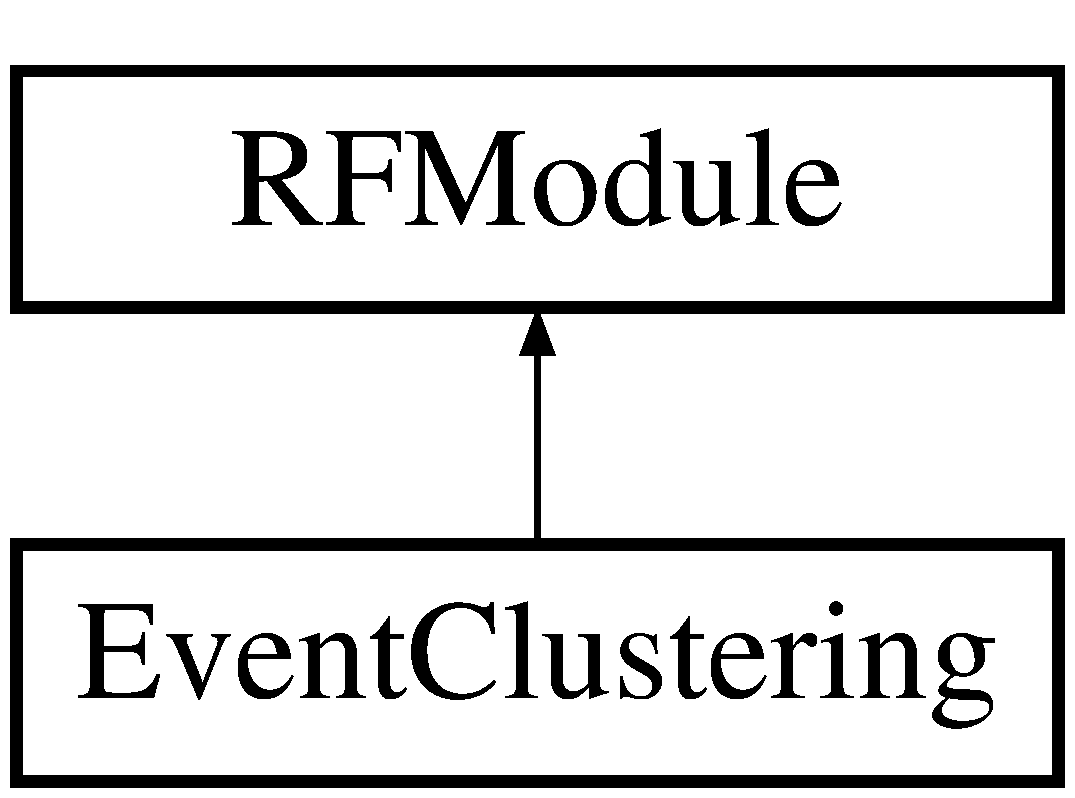
\includegraphics[height=2.000000cm]{classEventClustering}
\end{center}
\end{figure}
\subsection*{Public Member Functions}
\begin{DoxyCompactItemize}
\item 
bool {\bfseries configure} (yarp\+::os\+::\+Resource\+Finder \&rf)\hypertarget{classEventClustering_a9111f5db3d21a2a80bef0ac5a6996d06}{}\label{classEventClustering_a9111f5db3d21a2a80bef0ac5a6996d06}

\item 
bool {\bfseries interrupt\+Module} ()\hypertarget{classEventClustering_adb2bb1f480ac61629327d5170dd64398}{}\label{classEventClustering_adb2bb1f480ac61629327d5170dd64398}

\item 
bool {\bfseries close} ()\hypertarget{classEventClustering_af27e70c40cdfddab01c1fffed35620a3}{}\label{classEventClustering_af27e70c40cdfddab01c1fffed35620a3}

\item 
double {\bfseries get\+Period} ()\hypertarget{classEventClustering_afe356ead5fe50d67b2007e3f99f7818f}{}\label{classEventClustering_afe356ead5fe50d67b2007e3f99f7818f}

\item 
bool {\bfseries update\+Module} ()\hypertarget{classEventClustering_a25159637f1dc8c9cd27cde191b7296d2}{}\label{classEventClustering_a25159637f1dc8c9cd27cde191b7296d2}

\end{DoxyCompactItemize}


The documentation for this class was generated from the following files\+:\begin{DoxyCompactItemize}
\item 
/home/aglover/workspace/projects/event-\/driven/src/modules/v\+Cluster/include/event\+Clustering.\+h\item 
/home/aglover/workspace/projects/event-\/driven/src/modules/v\+Cluster/src/event\+Clustering.\+cpp\end{DoxyCompactItemize}

\hypertarget{classemorph_1_1eventProcessor}{}\section{emorph\+:\+:event\+Processor Class Reference}
\label{classemorph_1_1eventProcessor}\index{emorph\+::event\+Processor@{emorph\+::event\+Processor}}
\subsection*{Public Member Functions}
\begin{DoxyCompactItemize}
\item 
emorph\+::v\+Event \& {\bfseries my\+Func} (emorph\+::v\+Event \&event)\hypertarget{classemorph_1_1eventProcessor_a333c21041a0998eb2739900a0eb75752}{}\label{classemorph_1_1eventProcessor_a333c21041a0998eb2739900a0eb75752}

\end{DoxyCompactItemize}


The documentation for this class was generated from the following files\+:\begin{DoxyCompactItemize}
\item 
/home/aglover/workspace/projects/event-\/driven/src/modules/template/include/v\+Template\+Process.\+h\item 
/home/aglover/workspace/projects/event-\/driven/src/modules/template/src/v\+Template\+Process.\+cpp\end{DoxyCompactItemize}

\hypertarget{classeventStatisticsDumper}{}\section{event\+Statistics\+Dumper Class Reference}
\label{classeventStatisticsDumper}\index{event\+Statistics\+Dumper@{event\+Statistics\+Dumper}}
Inheritance diagram for event\+Statistics\+Dumper\+:\begin{figure}[H]
\begin{center}
\leavevmode
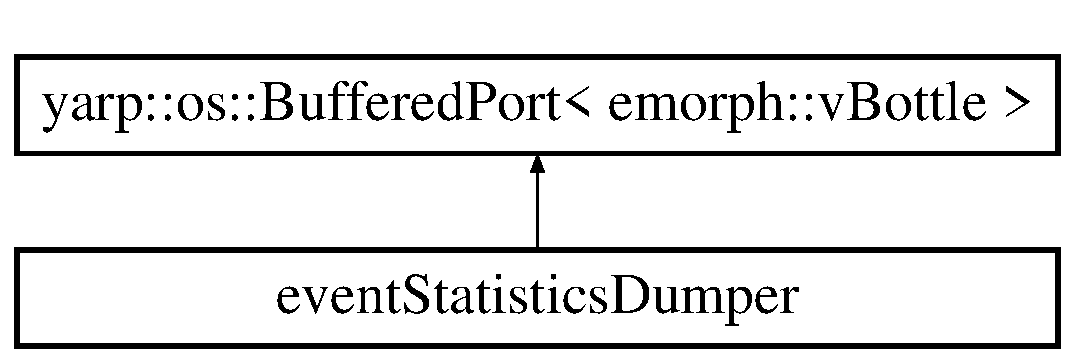
\includegraphics[height=2.000000cm]{classeventStatisticsDumper}
\end{center}
\end{figure}
\subsection*{Public Member Functions}
\begin{DoxyCompactItemize}
\item 
bool {\bfseries open} (std\+::string module\+Name=\char`\"{}E\+SD\char`\"{})\hypertarget{classeventStatisticsDumper_ae19ee350a1d131d0c54e0f7ac2437397}{}\label{classeventStatisticsDumper_ae19ee350a1d131d0c54e0f7ac2437397}

\item 
void {\bfseries on\+Read} (emorph\+::v\+Bottle \&bot)\hypertarget{classeventStatisticsDumper_a5373c7abee32f595308f59c3d2c02c01}{}\label{classeventStatisticsDumper_a5373c7abee32f595308f59c3d2c02c01}

\item 
void {\bfseries close} ()\hypertarget{classeventStatisticsDumper_aea5b77b83db3a9955e8fd8322d91dea1}{}\label{classeventStatisticsDumper_aea5b77b83db3a9955e8fd8322d91dea1}

\item 
void {\bfseries set\+Directory} (std\+::string dir)\hypertarget{classeventStatisticsDumper_a48c32b38d277f6b735c78cfbad6bcb64}{}\label{classeventStatisticsDumper_a48c32b38d277f6b735c78cfbad6bcb64}

\item 
int {\bfseries get\+Bottle\+Count} ()\hypertarget{classeventStatisticsDumper_af593efeee949a19d018aea33cbc5281a}{}\label{classeventStatisticsDumper_af593efeee949a19d018aea33cbc5281a}

\end{DoxyCompactItemize}


The documentation for this class was generated from the following files\+:\begin{DoxyCompactItemize}
\item 
/home/aglover/workspace/projects/event-\/driven/src/modules/v\+Analysis/include/event\+Analysis.\+h\item 
/home/aglover/workspace/projects/event-\/driven/src/modules/v\+Analysis/src/event\+Analysis.\+cpp\end{DoxyCompactItemize}

\hypertarget{classeventStatisticsModule}{}\section{event\+Statistics\+Module Class Reference}
\label{classeventStatisticsModule}\index{event\+Statistics\+Module@{event\+Statistics\+Module}}
Inheritance diagram for event\+Statistics\+Module\+:\begin{figure}[H]
\begin{center}
\leavevmode
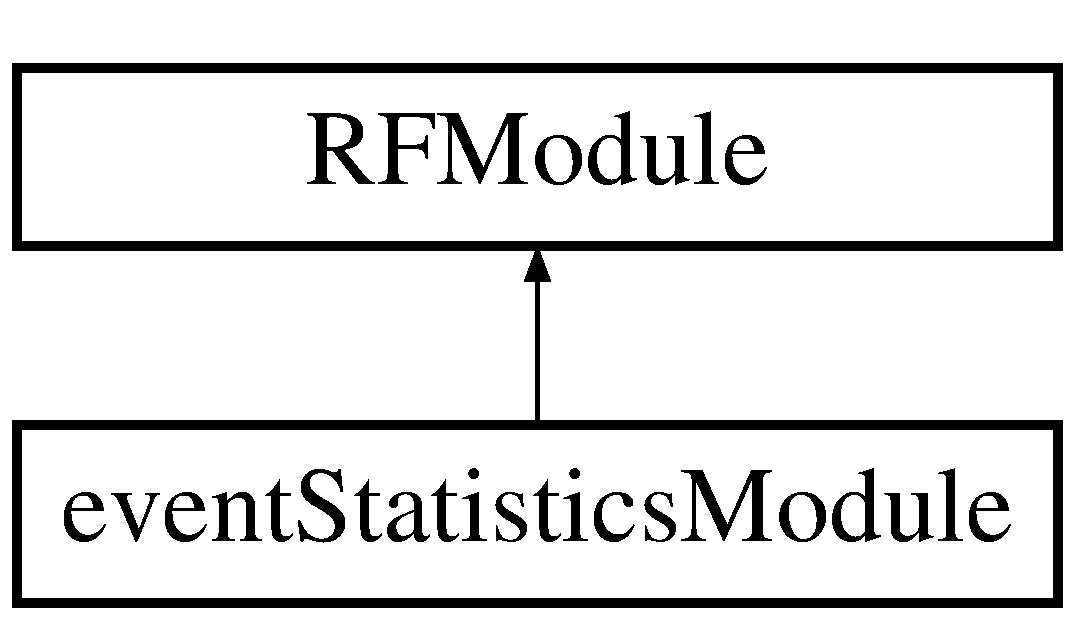
\includegraphics[height=2.000000cm]{classeventStatisticsModule}
\end{center}
\end{figure}
\subsection*{Public Member Functions}
\begin{DoxyCompactItemize}
\item 
bool {\bfseries configure} (yarp\+::os\+::\+Resource\+Finder \&rf)\hypertarget{classeventStatisticsModule_a1ca7b5499ca668297430d3976ce3b1d1}{}\label{classeventStatisticsModule_a1ca7b5499ca668297430d3976ce3b1d1}

\item 
bool {\bfseries close} ()\hypertarget{classeventStatisticsModule_ab11f4b9fdd8ec0d8f3aa0bcb415fef9c}{}\label{classeventStatisticsModule_ab11f4b9fdd8ec0d8f3aa0bcb415fef9c}

\item 
double {\bfseries get\+Period} ()\hypertarget{classeventStatisticsModule_a7e1825323f24dd316be0f7cb7eac80d2}{}\label{classeventStatisticsModule_a7e1825323f24dd316be0f7cb7eac80d2}

\item 
bool {\bfseries update\+Module} ()\hypertarget{classeventStatisticsModule_a08194f3ae070dc20ef93a403644ab5a6}{}\label{classeventStatisticsModule_a08194f3ae070dc20ef93a403644ab5a6}

\end{DoxyCompactItemize}


The documentation for this class was generated from the following files\+:\begin{DoxyCompactItemize}
\item 
/home/aglover/workspace/projects/event-\/driven/src/modules/v\+Analysis/include/event\+Analysis.\+h\item 
/home/aglover/workspace/projects/event-\/driven/src/modules/v\+Analysis/src/event\+Analysis.\+cpp\end{DoxyCompactItemize}

\hypertarget{classev_1_1fixedSurface}{}\section{ev\+:\+:fixed\+Surface Class Reference}
\label{classev_1_1fixedSurface}\index{ev\+::fixed\+Surface@{ev\+::fixed\+Surface}}
Inheritance diagram for ev\+:\+:fixed\+Surface\+:\begin{figure}[H]
\begin{center}
\leavevmode
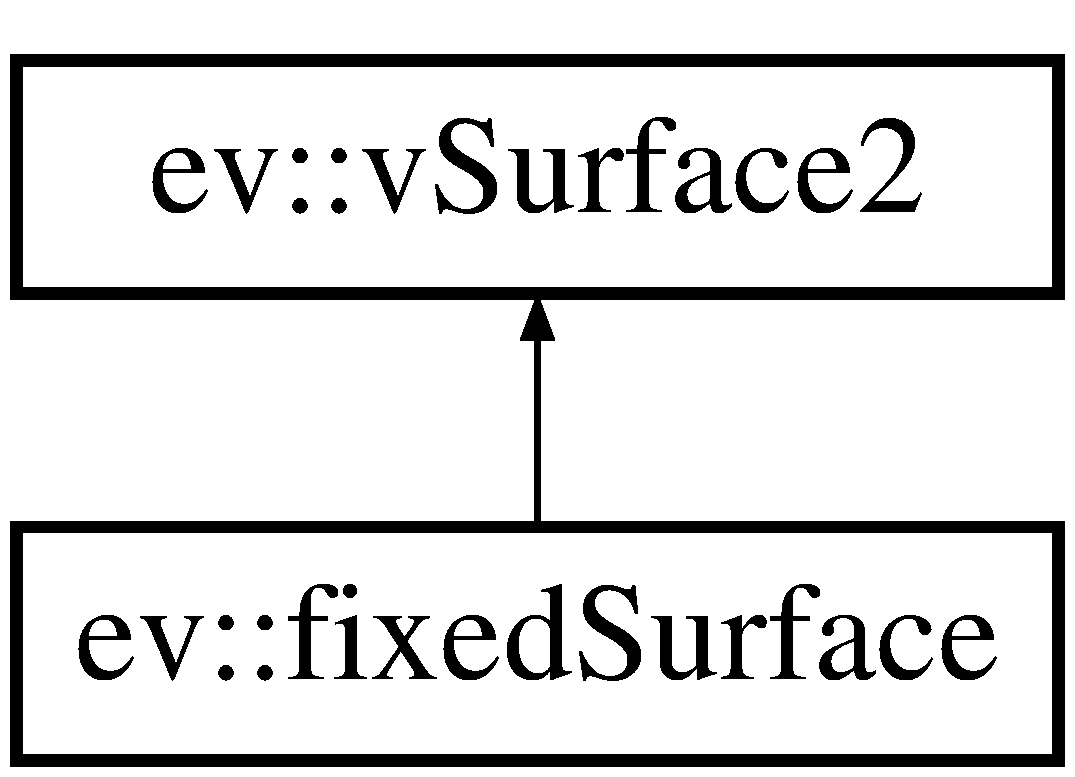
\includegraphics[height=2.000000cm]{classev_1_1fixedSurface}
\end{center}
\end{figure}
\subsection*{Public Member Functions}
\begin{DoxyCompactItemize}
\item 
{\bfseries fixed\+Surface} (int qlength=2000, int \hyperlink{classev_1_1vSurface2_a1aa8027816352a15d5b9bf1f26f48e76}{width}=128, int height=128)\hypertarget{classev_1_1fixedSurface_adee898e7c65c9c8d41fd20530d9f10b0}{}\label{classev_1_1fixedSurface_adee898e7c65c9c8d41fd20530d9f10b0}

\item 
virtual \hyperlink{classev_1_1vQueue}{v\+Queue} {\bfseries remove\+Events} (event$<$$>$ to\+Add)\hypertarget{classev_1_1fixedSurface_ace012acf57456f71d77fc7a349a915d7}{}\label{classev_1_1fixedSurface_ace012acf57456f71d77fc7a349a915d7}

\item 
void {\bfseries set\+Fixed\+Window\+Size} (int length)\hypertarget{classev_1_1fixedSurface_ac8249b63b5ada0491d6a6ff70b745488}{}\label{classev_1_1fixedSurface_ac8249b63b5ada0491d6a6ff70b745488}

\end{DoxyCompactItemize}
\subsection*{Additional Inherited Members}


The documentation for this class was generated from the following files\+:\begin{DoxyCompactItemize}
\item 
/home/aglover/workspace/projects/event-\/driven/libraries/include/i\+Cub/eventdriven/v\+Window.\+h\item 
/home/aglover/workspace/projects/event-\/driven/libraries/src/v\+Window.\+cpp\end{DoxyCompactItemize}

\hypertarget{classev_1_1FlowEvent}{}\section{ev\+:\+:Flow\+Event Class Reference}
\label{classev_1_1FlowEvent}\index{ev\+::\+Flow\+Event@{ev\+::\+Flow\+Event}}
Inheritance diagram for ev\+:\+:Flow\+Event\+:\begin{figure}[H]
\begin{center}
\leavevmode
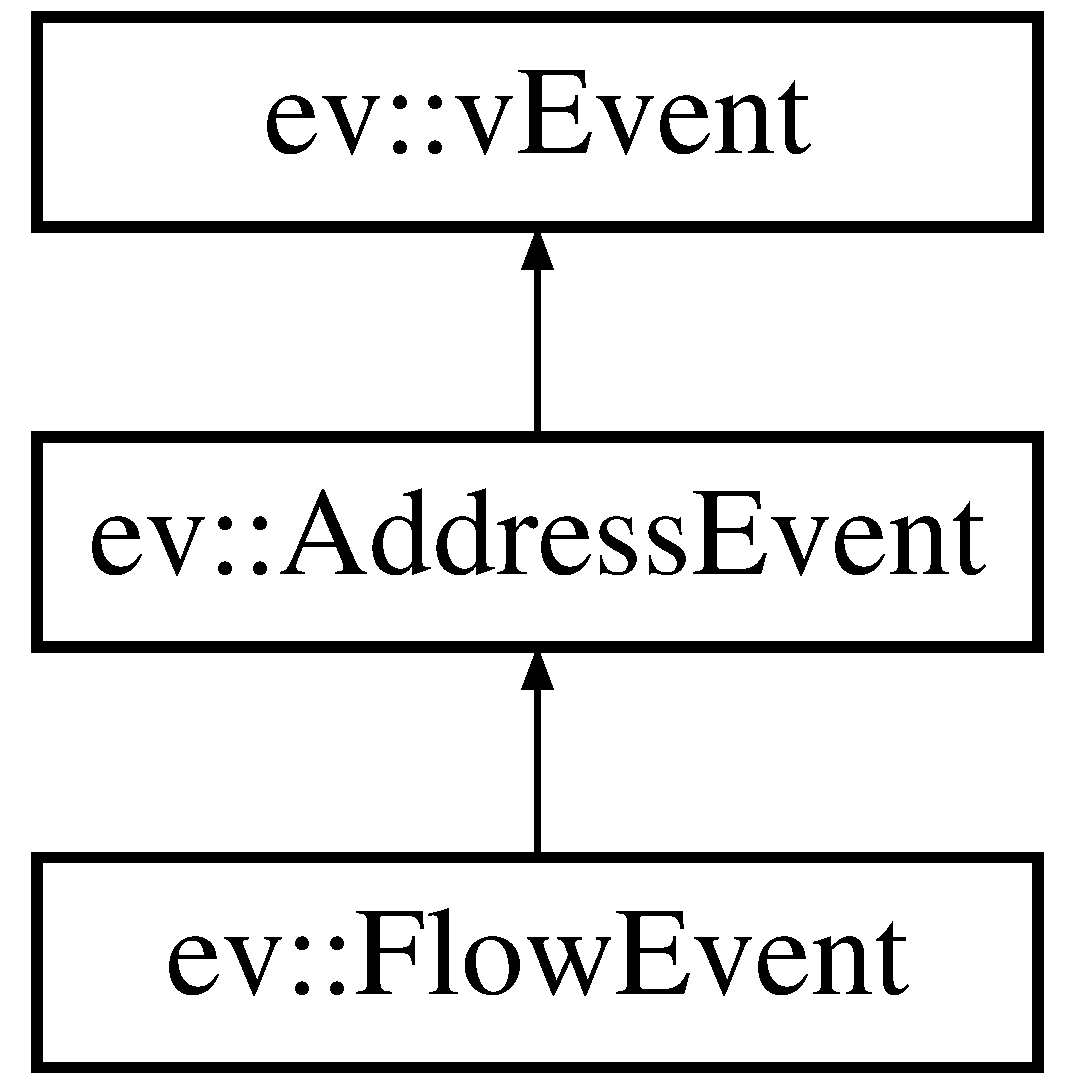
\includegraphics[height=3.000000cm]{classev_1_1FlowEvent}
\end{center}
\end{figure}
\subsection*{Public Member Functions}
\begin{DoxyCompactItemize}
\item 
virtual std\+::string {\bfseries get\+Type} () const \hypertarget{classev_1_1FlowEvent_a686886dc3a21091cdc5349c5fb4f7903}{}\label{classev_1_1FlowEvent_a686886dc3a21091cdc5349c5fb4f7903}

\item 
float {\bfseries get\+Vx} () const \hypertarget{classev_1_1FlowEvent_ae95bd90698da178c65781fdc05e6f482}{}\label{classev_1_1FlowEvent_ae95bd90698da178c65781fdc05e6f482}

\item 
float {\bfseries get\+Vy} () const \hypertarget{classev_1_1FlowEvent_a663ceac71491c60565a0e169dd4dbefa}{}\label{classev_1_1FlowEvent_a663ceac71491c60565a0e169dd4dbefa}

\item 
int {\bfseries get\+Death} () const \hypertarget{classev_1_1FlowEvent_ac39faf9016620faaddccd6c15b9f513f}{}\label{classev_1_1FlowEvent_ac39faf9016620faaddccd6c15b9f513f}

\item 
void {\bfseries set\+Vx} (float vx)\hypertarget{classev_1_1FlowEvent_a0691c4ac5178ef8f517d3e16fe5b6830}{}\label{classev_1_1FlowEvent_a0691c4ac5178ef8f517d3e16fe5b6830}

\item 
void {\bfseries set\+Vy} (float vy)\hypertarget{classev_1_1FlowEvent_a783ed251482b9c064c98b4e4351b3de6}{}\label{classev_1_1FlowEvent_a783ed251482b9c064c98b4e4351b3de6}

\item 
void {\bfseries set\+Death} ()\hypertarget{classev_1_1FlowEvent_af4eb95dd9a4326790daceb7685464a89}{}\label{classev_1_1FlowEvent_af4eb95dd9a4326790daceb7685464a89}

\item 
{\bfseries Flow\+Event} (const \hyperlink{classev_1_1vEvent}{v\+Event} \&event)\hypertarget{classev_1_1FlowEvent_afad4e2f7346e329102b6df806a828e39}{}\label{classev_1_1FlowEvent_afad4e2f7346e329102b6df806a828e39}

\item 
\hyperlink{classev_1_1vEvent}{v\+Event} \& {\bfseries operator=} (const \hyperlink{classev_1_1vEvent}{v\+Event} \&event)\hypertarget{classev_1_1FlowEvent_a6f4cc54ead8eab3a04f021efa280d087}{}\label{classev_1_1FlowEvent_a6f4cc54ead8eab3a04f021efa280d087}

\item 
virtual \hyperlink{classev_1_1vEvent}{v\+Event} $\ast$ {\bfseries clone} ()\hypertarget{classev_1_1FlowEvent_a9a1c52800ba95d9392026c42b153ee24}{}\label{classev_1_1FlowEvent_a9a1c52800ba95d9392026c42b153ee24}

\item 
bool {\bfseries operator==} (const \hyperlink{classev_1_1FlowEvent}{Flow\+Event} \&event)\hypertarget{classev_1_1FlowEvent_a85fb93e32e94718e5fb6a14bd85417e2}{}\label{classev_1_1FlowEvent_a85fb93e32e94718e5fb6a14bd85417e2}

\item 
bool {\bfseries operator==} (const \hyperlink{classev_1_1vEvent}{v\+Event} \&event)\hypertarget{classev_1_1FlowEvent_a29815a0c3a40e93c1b3087c29eb8b522}{}\label{classev_1_1FlowEvent_a29815a0c3a40e93c1b3087c29eb8b522}

\item 
virtual void {\bfseries encode} (yarp\+::os\+::\+Bottle \&b) const \hypertarget{classev_1_1FlowEvent_a13c900d7027a67d8197e32d56e92e0b0}{}\label{classev_1_1FlowEvent_a13c900d7027a67d8197e32d56e92e0b0}

\item 
yarp\+::os\+::\+Property {\bfseries get\+Content} () const \hypertarget{classev_1_1FlowEvent_a299486f89e1f893a513d237fd70ba00c}{}\label{classev_1_1FlowEvent_a299486f89e1f893a513d237fd70ba00c}

\item 
virtual bool {\bfseries decode} (const yarp\+::os\+::\+Bottle \&packet, int \&pos)\hypertarget{classev_1_1FlowEvent_a47a44a03752d3d0b5de668bfa8092d43}{}\label{classev_1_1FlowEvent_a47a44a03752d3d0b5de668bfa8092d43}

\item 
virtual int {\bfseries n\+Bytes\+Coded} () const \hypertarget{classev_1_1FlowEvent_a429953b6b4b849347295346a36950ce7}{}\label{classev_1_1FlowEvent_a429953b6b4b849347295346a36950ce7}

\end{DoxyCompactItemize}
\subsection*{Protected Attributes}
\begin{DoxyCompactItemize}
\item 
float {\bfseries vx}\hypertarget{classev_1_1FlowEvent_a614490d12ab9767e546e2929a4c7a65e}{}\label{classev_1_1FlowEvent_a614490d12ab9767e546e2929a4c7a65e}

\item 
float {\bfseries vy}\hypertarget{classev_1_1FlowEvent_a20416e333c9f0258a2a1bbb49fb14989}{}\label{classev_1_1FlowEvent_a20416e333c9f0258a2a1bbb49fb14989}

\item 
int {\bfseries death}\hypertarget{classev_1_1FlowEvent_ae6b074315c90ad3e1fbc8a6d76cbdcbe}{}\label{classev_1_1FlowEvent_ae6b074315c90ad3e1fbc8a6d76cbdcbe}

\end{DoxyCompactItemize}


The documentation for this class was generated from the following files\+:\begin{DoxyCompactItemize}
\item 
/home/aglover/workspace/projects/event-\/driven/libraries/include/i\+Cub/eventdriven/v\+Codec.\+h\item 
/home/aglover/workspace/projects/event-\/driven/libraries/src/v\+Codec.\+cpp\end{DoxyCompactItemize}

\hypertarget{structfpgaStatus}{}\section{fpga\+Status Struct Reference}
\label{structfpgaStatus}\index{fpga\+Status@{fpga\+Status}}
\subsection*{Public Attributes}
\begin{DoxyCompactItemize}
\item 
bool {\bfseries crc\+Err}\hypertarget{structfpgaStatus_a9cafcfd4e38fa240b31b47611bac3083}{}\label{structfpgaStatus_a9cafcfd4e38fa240b31b47611bac3083}

\item 
bool {\bfseries bias\+Done}\hypertarget{structfpgaStatus_aef80b6cd223b1195b317a70e7f57b58c}{}\label{structfpgaStatus_aef80b6cd223b1195b317a70e7f57b58c}

\item 
bool {\bfseries i2c\+Timeout}\hypertarget{structfpgaStatus_ab37e07a6f39e462634df9d560c0abe45}{}\label{structfpgaStatus_ab37e07a6f39e462634df9d560c0abe45}

\item 
bool {\bfseries aps\+Fifo\+Full}\hypertarget{structfpgaStatus_a01141df5867a1c152efd241a5341cfb7}{}\label{structfpgaStatus_a01141df5867a1c152efd241a5341cfb7}

\item 
bool {\bfseries td\+Fifo\+Full}\hypertarget{structfpgaStatus_a432c220a53f8a0639cb2b0ef1284ef14}{}\label{structfpgaStatus_a432c220a53f8a0639cb2b0ef1284ef14}

\end{DoxyCompactItemize}


The documentation for this struct was generated from the following file\+:\begin{DoxyCompactItemize}
\item 
/home/aglover/workspace/projects/event-\/driven/src/hardwareio/zynq\+Grabber/include/device\+Controller.\+h\end{DoxyCompactItemize}

\hypertarget{classev_1_1InterestEvent}{}\section{ev\+:\+:Interest\+Event Class Reference}
\label{classev_1_1InterestEvent}\index{ev\+::\+Interest\+Event@{ev\+::\+Interest\+Event}}
Inheritance diagram for ev\+:\+:Interest\+Event\+:\begin{figure}[H]
\begin{center}
\leavevmode
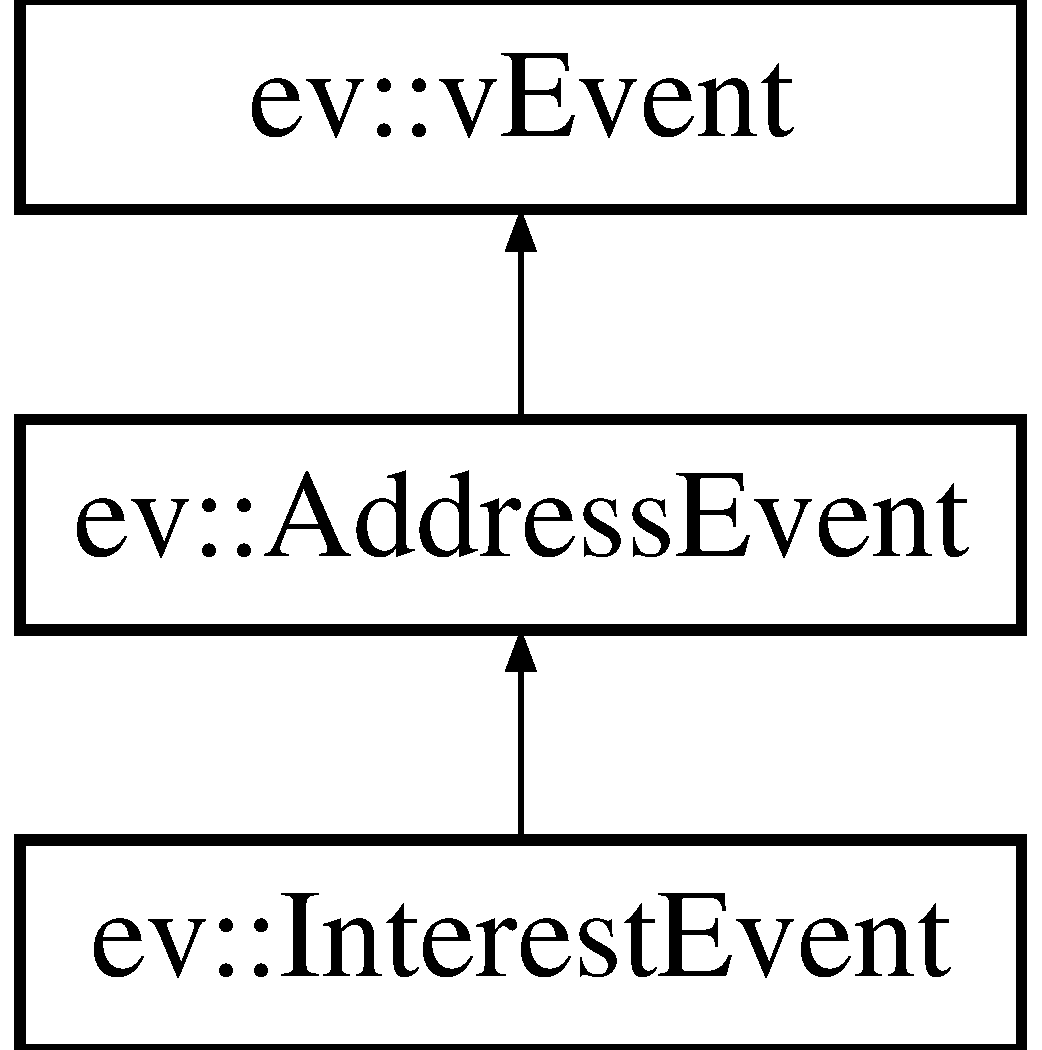
\includegraphics[height=3.000000cm]{classev_1_1InterestEvent}
\end{center}
\end{figure}
\subsection*{Public Member Functions}
\begin{DoxyCompactItemize}
\item 
virtual std\+::string {\bfseries get\+Type} () const \hypertarget{classev_1_1InterestEvent_a63fdfcabfca0ecf0554eccb1eadda751}{}\label{classev_1_1InterestEvent_a63fdfcabfca0ecf0554eccb1eadda751}

\item 
int {\bfseries get\+ID} () const \hypertarget{classev_1_1InterestEvent_a045f85bd13470efe93904275a9da5c1b}{}\label{classev_1_1InterestEvent_a045f85bd13470efe93904275a9da5c1b}

\item 
void {\bfseries set\+ID} (const int int\+ID)\hypertarget{classev_1_1InterestEvent_acbb2eb34db2594d80b9aade51eb9ff7b}{}\label{classev_1_1InterestEvent_acbb2eb34db2594d80b9aade51eb9ff7b}

\item 
{\bfseries Interest\+Event} (const \hyperlink{classev_1_1vEvent}{v\+Event} \&event)\hypertarget{classev_1_1InterestEvent_a660a459a68d4d7d86436a6af0fdb98c6}{}\label{classev_1_1InterestEvent_a660a459a68d4d7d86436a6af0fdb98c6}

\item 
\hyperlink{classev_1_1vEvent}{v\+Event} \& {\bfseries operator=} (const \hyperlink{classev_1_1vEvent}{v\+Event} \&event)\hypertarget{classev_1_1InterestEvent_a3194622867f847b78867035595a23eb2}{}\label{classev_1_1InterestEvent_a3194622867f847b78867035595a23eb2}

\item 
virtual \hyperlink{classev_1_1vEvent}{v\+Event} $\ast$ {\bfseries clone} ()\hypertarget{classev_1_1InterestEvent_aad82d9299e6cc1fadd86c2620e97b7cd}{}\label{classev_1_1InterestEvent_aad82d9299e6cc1fadd86c2620e97b7cd}

\item 
bool {\bfseries operator==} (const \hyperlink{classev_1_1InterestEvent}{Interest\+Event} \&event)\hypertarget{classev_1_1InterestEvent_ace17bdbe6bfd2e1ca5ed9a9a9ea0fab0}{}\label{classev_1_1InterestEvent_ace17bdbe6bfd2e1ca5ed9a9a9ea0fab0}

\item 
bool {\bfseries operator==} (const \hyperlink{classev_1_1vEvent}{v\+Event} \&event)\hypertarget{classev_1_1InterestEvent_ab88e5cfcb71a211216f295b67db7ecdc}{}\label{classev_1_1InterestEvent_ab88e5cfcb71a211216f295b67db7ecdc}

\item 
virtual void {\bfseries encode} (yarp\+::os\+::\+Bottle \&b) const \hypertarget{classev_1_1InterestEvent_a4a0106bc9e49bc7439402f85531f3e05}{}\label{classev_1_1InterestEvent_a4a0106bc9e49bc7439402f85531f3e05}

\item 
yarp\+::os\+::\+Property {\bfseries get\+Content} () const \hypertarget{classev_1_1InterestEvent_a24fcac627ac04495434bc5f41b2bbe88}{}\label{classev_1_1InterestEvent_a24fcac627ac04495434bc5f41b2bbe88}

\item 
virtual bool {\bfseries decode} (const yarp\+::os\+::\+Bottle \&packet, int \&pos)\hypertarget{classev_1_1InterestEvent_a4e1d28f09a9e4e75a7e9019c37bfe3ad}{}\label{classev_1_1InterestEvent_a4e1d28f09a9e4e75a7e9019c37bfe3ad}

\item 
virtual int {\bfseries n\+Bytes\+Coded} () const \hypertarget{classev_1_1InterestEvent_aebd398321f2b4dc3f04a94c7d96802f2}{}\label{classev_1_1InterestEvent_aebd398321f2b4dc3f04a94c7d96802f2}

\end{DoxyCompactItemize}
\subsection*{Protected Attributes}
\begin{DoxyCompactItemize}
\item 
int {\bfseries int\+ID}\hypertarget{classev_1_1InterestEvent_ab71373afcb8a966d3cef8b91f31d114f}{}\label{classev_1_1InterestEvent_ab71373afcb8a966d3cef8b91f31d114f}

\end{DoxyCompactItemize}


The documentation for this class was generated from the following files\+:\begin{DoxyCompactItemize}
\item 
/home/aglover/workspace/projects/event-\/driven/libraries/include/i\+Cub/eventdriven/v\+Codec.\+h\item 
/home/aglover/workspace/projects/event-\/driven/libraries/src/v\+Codec.\+cpp\end{DoxyCompactItemize}

\hypertarget{classev_1_1lifetimeSurface}{}\section{ev\+:\+:lifetime\+Surface Class Reference}
\label{classev_1_1lifetimeSurface}\index{ev\+::lifetime\+Surface@{ev\+::lifetime\+Surface}}
Inheritance diagram for ev\+:\+:lifetime\+Surface\+:\begin{figure}[H]
\begin{center}
\leavevmode
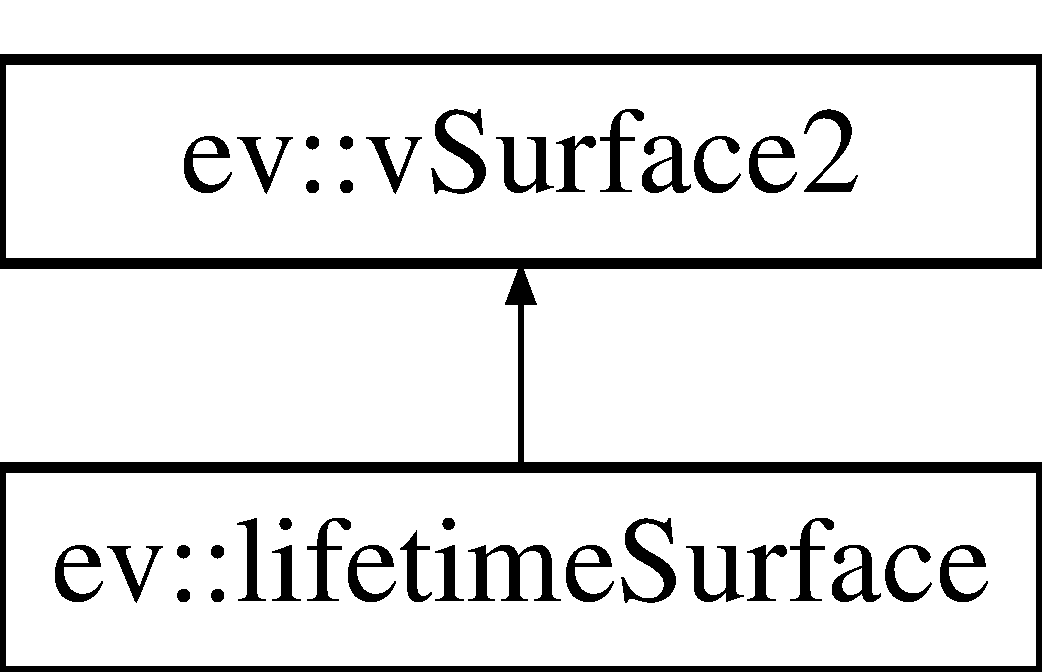
\includegraphics[height=2.000000cm]{classev_1_1lifetimeSurface}
\end{center}
\end{figure}
\subsection*{Public Member Functions}
\begin{DoxyCompactItemize}
\item 
{\bfseries lifetime\+Surface} (int \hyperlink{classev_1_1vSurface2_a1aa8027816352a15d5b9bf1f26f48e76}{width}=128, int height=128)\hypertarget{classev_1_1lifetimeSurface_a8276286d48b5baf2829268333f99b482}{}\label{classev_1_1lifetimeSurface_a8276286d48b5baf2829268333f99b482}

\item 
virtual \hyperlink{classev_1_1vQueue}{v\+Queue} \hyperlink{classev_1_1lifetimeSurface_a8fce037a13281c0e46c7d660e0ea2275}{add\+Event} (event$<$$>$ to\+Add)
\begin{DoxyCompactList}\small\item\em add\+Event adds an event to the window. Also checks for expired events. \end{DoxyCompactList}\item 
virtual \hyperlink{classev_1_1vQueue}{v\+Queue} {\bfseries remove\+Events} (event$<$$>$ to\+Add)\hypertarget{classev_1_1lifetimeSurface_a86fde904d007b5b1e5f52351bfab0b17}{}\label{classev_1_1lifetimeSurface_a86fde904d007b5b1e5f52351bfab0b17}

\end{DoxyCompactItemize}
\subsection*{Additional Inherited Members}


\subsection{Member Function Documentation}
\index{ev\+::lifetime\+Surface@{ev\+::lifetime\+Surface}!add\+Event@{add\+Event}}
\index{add\+Event@{add\+Event}!ev\+::lifetime\+Surface@{ev\+::lifetime\+Surface}}
\subsubsection[{\texorpdfstring{add\+Event(event$<$$>$ to\+Add)}{addEvent(event<> toAdd)}}]{\setlength{\rightskip}{0pt plus 5cm}{\bf v\+Queue} ev\+::lifetime\+Surface\+::add\+Event (
\begin{DoxyParamCaption}
\item[{event$<$$>$}]{v}
\end{DoxyParamCaption}
)\hspace{0.3cm}{\ttfamily [virtual]}}\hypertarget{classev_1_1lifetimeSurface_a8fce037a13281c0e46c7d660e0ea2275}{}\label{classev_1_1lifetimeSurface_a8fce037a13281c0e46c7d660e0ea2275}


add\+Event adds an event to the window. Also checks for expired events. 


\begin{DoxyParams}{Parameters}
{\em event} & the event to add \\
\hline
\end{DoxyParams}


Reimplemented from \hyperlink{classev_1_1vSurface2_a6dee662976048b73d7b19e45871352da}{ev\+::v\+Surface2}.



The documentation for this class was generated from the following files\+:\begin{DoxyCompactItemize}
\item 
/home/aglover/workspace/projects/event-\/driven/libraries/include/i\+Cub/eventdriven/v\+Window.\+h\item 
/home/aglover/workspace/projects/event-\/driven/libraries/src/v\+Window.\+cpp\end{DoxyCompactItemize}

\hypertarget{classev_1_1NeuronIDEvent}{}\section{ev\+:\+:Neuron\+I\+D\+Event Class Reference}
\label{classev_1_1NeuronIDEvent}\index{ev\+::\+Neuron\+I\+D\+Event@{ev\+::\+Neuron\+I\+D\+Event}}
Inheritance diagram for ev\+:\+:Neuron\+I\+D\+Event\+:\begin{figure}[H]
\begin{center}
\leavevmode
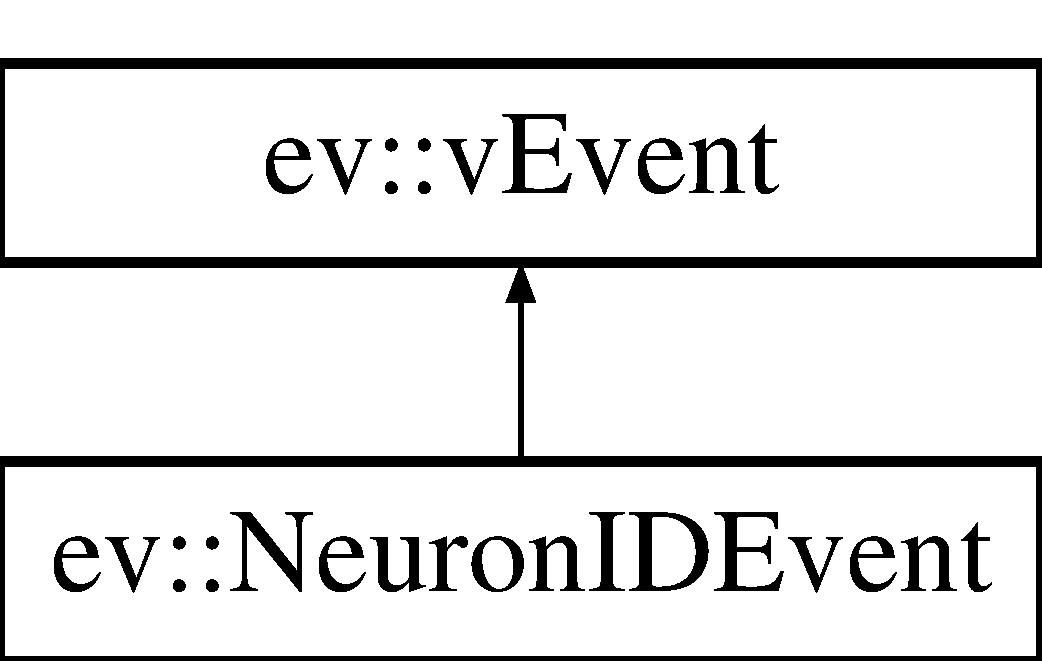
\includegraphics[height=2.000000cm]{classev_1_1NeuronIDEvent}
\end{center}
\end{figure}
\subsection*{Public Member Functions}
\begin{DoxyCompactItemize}
\item 
virtual std\+::string {\bfseries get\+Type} () const \hypertarget{classev_1_1NeuronIDEvent_a71548e0a5b42fb693050da5f615e83fd}{}\label{classev_1_1NeuronIDEvent_a71548e0a5b42fb693050da5f615e83fd}

\item 
int {\bfseries get\+ID} () const \hypertarget{classev_1_1NeuronIDEvent_ae86cefbe2983c8793c3509e620b44036}{}\label{classev_1_1NeuronIDEvent_ae86cefbe2983c8793c3509e620b44036}

\item 
void {\bfseries set\+ID} (const int neur\+ID)\hypertarget{classev_1_1NeuronIDEvent_ad843c27bca4d310819f3cf756b29089d}{}\label{classev_1_1NeuronIDEvent_ad843c27bca4d310819f3cf756b29089d}

\item 
{\bfseries Neuron\+I\+D\+Event} (const \hyperlink{classev_1_1vEvent}{v\+Event} \&event)\hypertarget{classev_1_1NeuronIDEvent_a6b08dbb4ac55a13528f6f43e7259987f}{}\label{classev_1_1NeuronIDEvent_a6b08dbb4ac55a13528f6f43e7259987f}

\item 
\hyperlink{classev_1_1vEvent}{v\+Event} \& {\bfseries operator=} (const \hyperlink{classev_1_1vEvent}{v\+Event} \&event)\hypertarget{classev_1_1NeuronIDEvent_a705884450f2883b6398ef8608fb33c37}{}\label{classev_1_1NeuronIDEvent_a705884450f2883b6398ef8608fb33c37}

\item 
virtual \hyperlink{classev_1_1vEvent}{v\+Event} $\ast$ {\bfseries clone} ()\hypertarget{classev_1_1NeuronIDEvent_aa0054775d211f072cd0aec353fb7ef1a}{}\label{classev_1_1NeuronIDEvent_aa0054775d211f072cd0aec353fb7ef1a}

\item 
bool {\bfseries operator==} (const \hyperlink{classev_1_1NeuronIDEvent}{Neuron\+I\+D\+Event} \&event)\hypertarget{classev_1_1NeuronIDEvent_a5478799d323fc588787aef446ddca511}{}\label{classev_1_1NeuronIDEvent_a5478799d323fc588787aef446ddca511}

\item 
bool {\bfseries operator==} (const \hyperlink{classev_1_1vEvent}{v\+Event} \&event)\hypertarget{classev_1_1NeuronIDEvent_a4d105c1883a059e54a9c270e9b1fa687}{}\label{classev_1_1NeuronIDEvent_a4d105c1883a059e54a9c270e9b1fa687}

\item 
virtual void {\bfseries encode} (yarp\+::os\+::\+Bottle \&b) const \hypertarget{classev_1_1NeuronIDEvent_a6b2fcf1d4e19bf5c281562764cdd2cbe}{}\label{classev_1_1NeuronIDEvent_a6b2fcf1d4e19bf5c281562764cdd2cbe}

\item 
yarp\+::os\+::\+Property {\bfseries get\+Content} () const \hypertarget{classev_1_1NeuronIDEvent_abef9ad9b422ac7740f6744bd7c800414}{}\label{classev_1_1NeuronIDEvent_abef9ad9b422ac7740f6744bd7c800414}

\item 
virtual bool {\bfseries decode} (const yarp\+::os\+::\+Bottle \&packet, int \&pos)\hypertarget{classev_1_1NeuronIDEvent_ae4ab33a0b6fdaa77a8d938d903da19ee}{}\label{classev_1_1NeuronIDEvent_ae4ab33a0b6fdaa77a8d938d903da19ee}

\item 
virtual int {\bfseries n\+Bytes\+Coded} () const \hypertarget{classev_1_1NeuronIDEvent_ad5281fe1a0e4da49adfb5f1110756eec}{}\label{classev_1_1NeuronIDEvent_ad5281fe1a0e4da49adfb5f1110756eec}

\end{DoxyCompactItemize}
\subsection*{Protected Attributes}
\begin{DoxyCompactItemize}
\item 
int {\bfseries neur\+ID}\hypertarget{classev_1_1NeuronIDEvent_a6d52d929d7194a617a07a954e1ba3fa8}{}\label{classev_1_1NeuronIDEvent_a6d52d929d7194a617a07a954e1ba3fa8}

\end{DoxyCompactItemize}


The documentation for this class was generated from the following files\+:\begin{DoxyCompactItemize}
\item 
/home/aglover/workspace/projects/event-\/driven/libraries/include/i\+Cub/eventdriven/v\+Codec.\+h\item 
/home/aglover/workspace/projects/event-\/driven/libraries/src/v\+Codec.\+cpp\end{DoxyCompactItemize}

\hypertarget{classparticleProcessor}{}\section{particle\+Processor Class Reference}
\label{classparticleProcessor}\index{particle\+Processor@{particle\+Processor}}
Inheritance diagram for particle\+Processor\+:\begin{figure}[H]
\begin{center}
\leavevmode
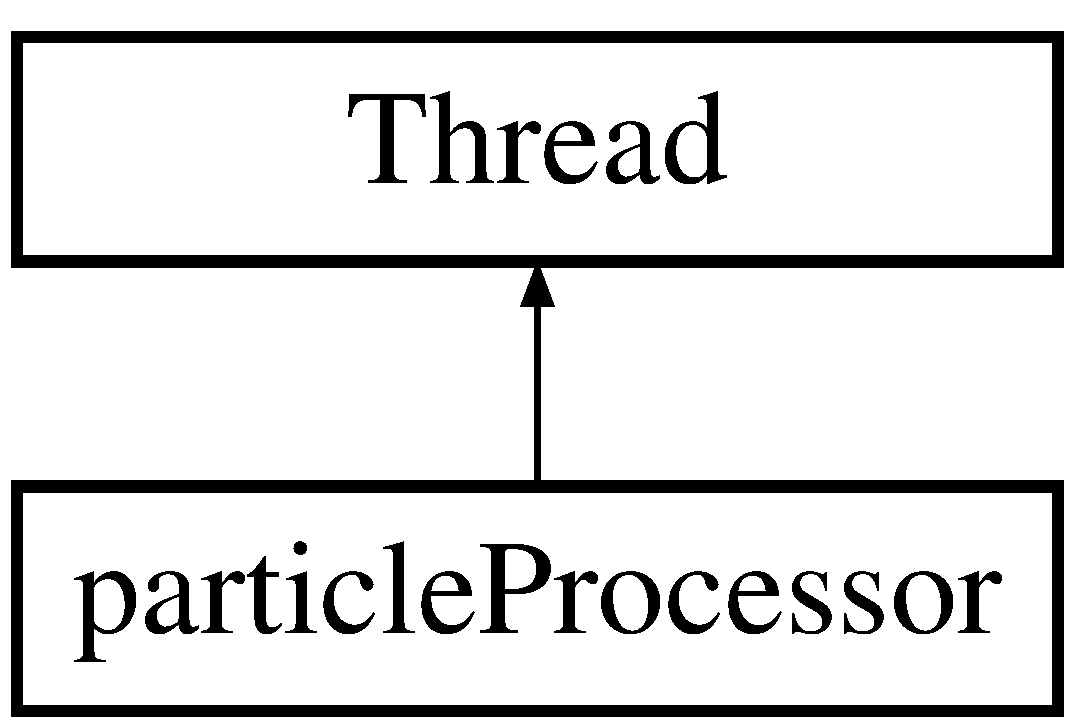
\includegraphics[height=2.000000cm]{classparticleProcessor}
\end{center}
\end{figure}
\subsection*{Public Member Functions}
\begin{DoxyCompactItemize}
\item 
{\bfseries particle\+Processor} (unsigned int height, unsigned int width, std\+::string name, bool strict)\hypertarget{classparticleProcessor_af03a74f1518329726ae2e5e1ec92ee01}{}\label{classparticleProcessor_af03a74f1518329726ae2e5e1ec92ee01}

\item 
bool {\bfseries thread\+Init} ()\hypertarget{classparticleProcessor_aafa6595892c7e82b1c42b919dfe6f9f0}{}\label{classparticleProcessor_aafa6595892c7e82b1c42b919dfe6f9f0}

\item 
void {\bfseries run} ()\hypertarget{classparticleProcessor_aed880e77fafb61965d57565735939181}{}\label{classparticleProcessor_aed880e77fafb61965d57565735939181}

\item 
void {\bfseries thread\+Release} ()\hypertarget{classparticleProcessor_ae40c3b11945587c4c23547d7b817299a}{}\label{classparticleProcessor_ae40c3b11945587c4c23547d7b817299a}

\end{DoxyCompactItemize}


The documentation for this class was generated from the following files\+:\begin{DoxyCompactItemize}
\item 
/home/aglover/workspace/projects/event-\/driven/src/modules/v\+Particle\+Filter/include/v\+Particle\+Module.\+h\item 
/home/aglover/workspace/projects/event-\/driven/src/modules/v\+Particle\+Filter/src/v\+Particle\+Module.\+cpp\end{DoxyCompactItemize}

\hypertarget{structev_1_1resolution}{}\section{ev\+:\+:resolution Struct Reference}
\label{structev_1_1resolution}\index{ev\+::resolution@{ev\+::resolution}}
\subsection*{Public Attributes}
\begin{DoxyCompactItemize}
\item 
unsigned int {\bfseries width}\+:10\hypertarget{structev_1_1resolution_af63d9f023bf48b5170fbde6fac1fa60d}{}\label{structev_1_1resolution_af63d9f023bf48b5170fbde6fac1fa60d}

\item 
unsigned int {\bfseries height}\+:10\hypertarget{structev_1_1resolution_ae9919e691ce05e1bbbf281dd79102ddb}{}\label{structev_1_1resolution_ae9919e691ce05e1bbbf281dd79102ddb}

\end{DoxyCompactItemize}


The documentation for this struct was generated from the following file\+:\begin{DoxyCompactItemize}
\item 
/home/aglover/workspace/projects/event-\/driven/libraries/include/i\+Cub/eventdriven/vts\+Helper.\+h\end{DoxyCompactItemize}

\hypertarget{classsaccadeModule}{}\section{saccade\+Module Class Reference}
\label{classsaccadeModule}\index{saccade\+Module@{saccade\+Module}}
Inheritance diagram for saccade\+Module\+:\begin{figure}[H]
\begin{center}
\leavevmode
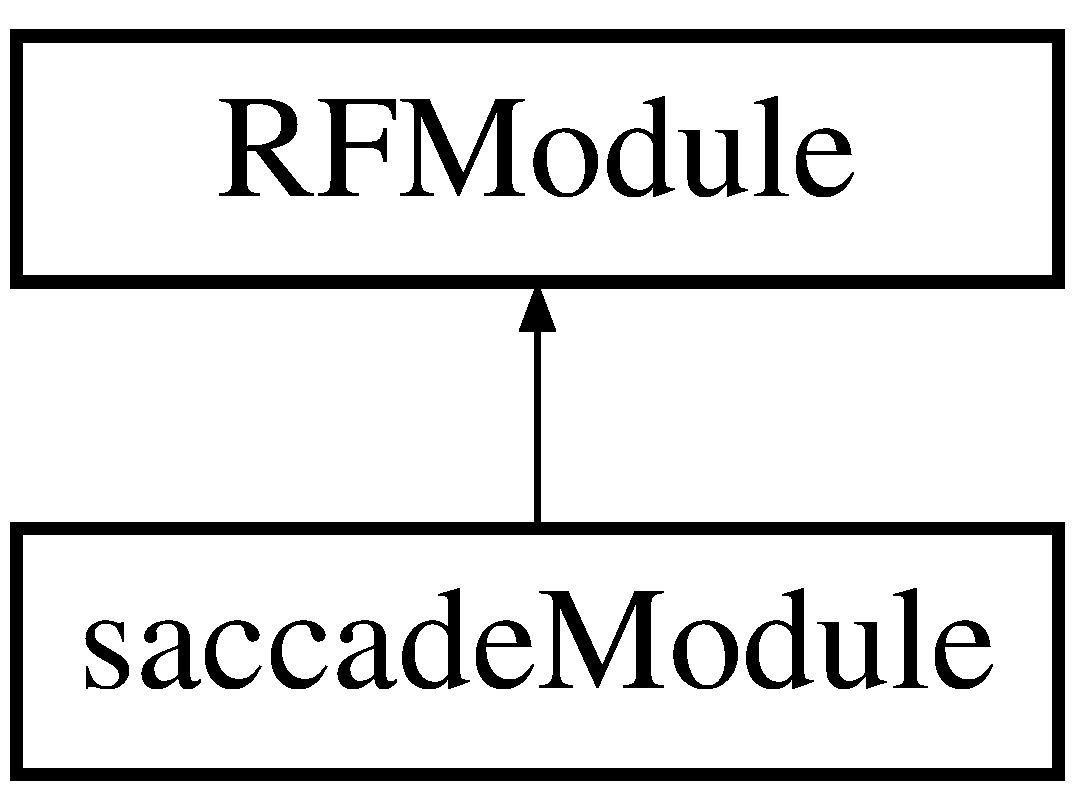
\includegraphics[height=2.000000cm]{classsaccadeModule}
\end{center}
\end{figure}
\subsection*{Public Member Functions}
\begin{DoxyCompactItemize}
\item 
virtual bool {\bfseries configure} (yarp\+::os\+::\+Resource\+Finder \&rf)\hypertarget{classsaccadeModule_aad1f5d8c2f33c4c9dadb8e015de9cafc}{}\label{classsaccadeModule_aad1f5d8c2f33c4c9dadb8e015de9cafc}

\item 
virtual bool {\bfseries interrupt\+Module} ()\hypertarget{classsaccadeModule_ac249486e8d00cdb52ec316c5665032ee}{}\label{classsaccadeModule_ac249486e8d00cdb52ec316c5665032ee}

\item 
virtual bool {\bfseries close} ()\hypertarget{classsaccadeModule_a510ff21af86c5ccf330cf334e63d0f4f}{}\label{classsaccadeModule_a510ff21af86c5ccf330cf334e63d0f4f}

\item 
virtual bool {\bfseries respond} (const yarp\+::os\+::\+Bottle \&command, yarp\+::os\+::\+Bottle \&reply)\hypertarget{classsaccadeModule_a4392d2dc4f60014da07b12772f216430}{}\label{classsaccadeModule_a4392d2dc4f60014da07b12772f216430}

\item 
virtual double {\bfseries get\+Period} ()\hypertarget{classsaccadeModule_a8e603e09181d0cf26b020e6808b9a120}{}\label{classsaccadeModule_a8e603e09181d0cf26b020e6808b9a120}

\item 
virtual bool {\bfseries update\+Module} ()\hypertarget{classsaccadeModule_abb6ee7b679476de9ff75d78b75709e9d}{}\label{classsaccadeModule_abb6ee7b679476de9ff75d78b75709e9d}

\end{DoxyCompactItemize}


The documentation for this class was generated from the following files\+:\begin{DoxyCompactItemize}
\item 
/home/aglover/workspace/projects/event-\/driven/src/robotio/autosaccade/include/auto\+Saccade.\+h\item 
/home/aglover/workspace/projects/event-\/driven/src/robotio/autosaccade/src/auto\+Saccade.\+cpp\end{DoxyCompactItemize}

\hypertarget{classsendingBuffer}{}\section{sending\+Buffer Class Reference}
\label{classsendingBuffer}\index{sending\+Buffer@{sending\+Buffer}}
Inheritance diagram for sending\+Buffer\+:\begin{figure}[H]
\begin{center}
\leavevmode
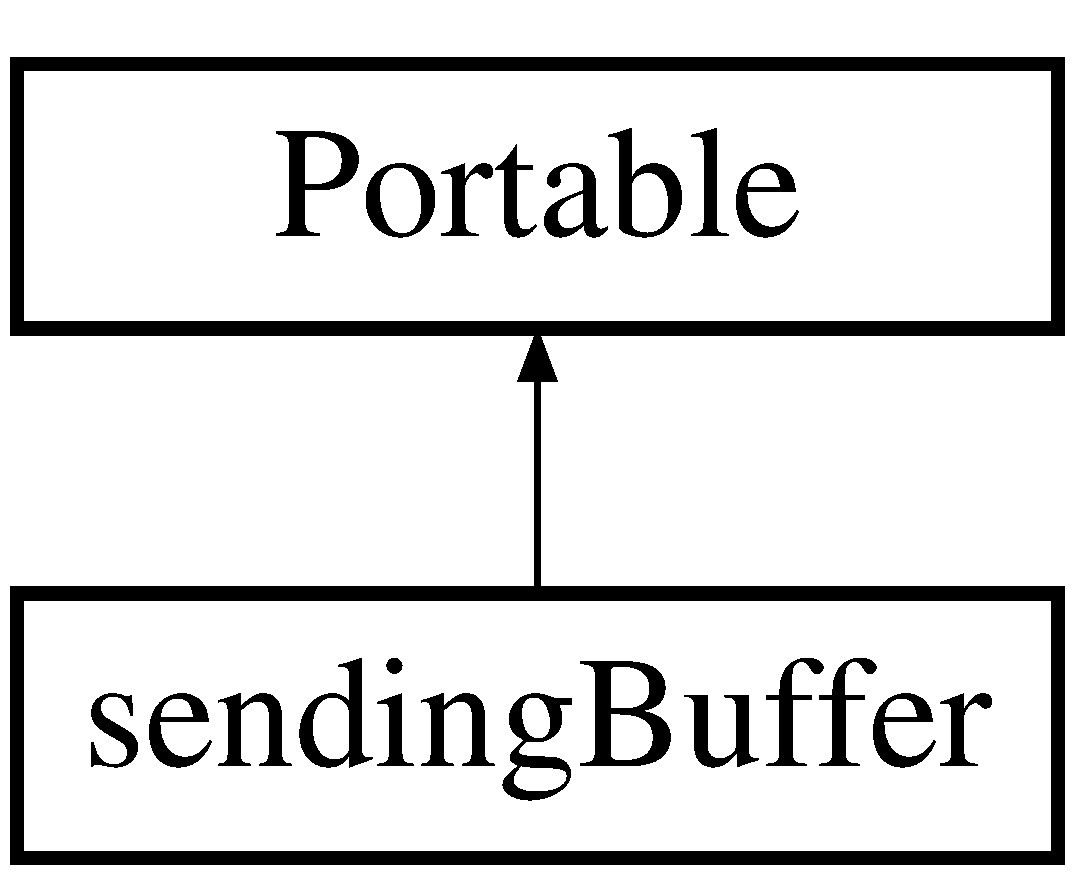
\includegraphics[height=2.000000cm]{classsendingBuffer}
\end{center}
\end{figure}
\subsection*{Public Member Functions}
\begin{DoxyCompactItemize}
\item 
{\bfseries sending\+Buffer} (char $\ast$, int)\hypertarget{classsendingBuffer_ab4c1d25d2e85e15f48e06873097deaa2}{}\label{classsendingBuffer_ab4c1d25d2e85e15f48e06873097deaa2}

\item 
virtual bool {\bfseries write} (yarp\+::os\+::\+Connection\+Writer \&)\hypertarget{classsendingBuffer_a40b2e61a078ebe6ea507afd73728f82c}{}\label{classsendingBuffer_a40b2e61a078ebe6ea507afd73728f82c}

\item 
virtual bool {\bfseries read} (yarp\+::os\+::\+Connection\+Reader \&)\hypertarget{classsendingBuffer_ad148ea47f1ef7d56e522909c212ae552}{}\label{classsendingBuffer_ad148ea47f1ef7d56e522909c212ae552}

\item 
void {\bfseries set\+\_\+data} (char $\ast$, int)\hypertarget{classsendingBuffer_adf6ced8e177d52765bc8504af4aa0a45}{}\label{classsendingBuffer_adf6ced8e177d52765bc8504af4aa0a45}

\item 
char $\ast$ {\bfseries get\+\_\+packet} ()\hypertarget{classsendingBuffer_a81ead3fede32e415e1073f31d9bc2f43}{}\label{classsendingBuffer_a81ead3fede32e415e1073f31d9bc2f43}

\item 
int {\bfseries get\+\_\+size\+Of\+Packet} ()\hypertarget{classsendingBuffer_a76aaef5c8f64d644c04536a9dbb75de6}{}\label{classsendingBuffer_a76aaef5c8f64d644c04536a9dbb75de6}

\end{DoxyCompactItemize}


The documentation for this class was generated from the following files\+:\begin{DoxyCompactItemize}
\item 
/home/aglover/workspace/projects/event-\/driven/src/hardwareio/aex\+Grabber/include/\hyperlink{sending__buffer_8h}{sending\+\_\+buffer.\+h}\item 
/home/aglover/workspace/projects/event-\/driven/src/hardwareio/aex\+Grabber/src/sending\+\_\+buffer.\+cpp\end{DoxyCompactItemize}

\hypertarget{classspinconverterModule}{}\section{spinconverter\+Module Class Reference}
\label{classspinconverterModule}\index{spinconverter\+Module@{spinconverter\+Module}}
Inheritance diagram for spinconverter\+Module\+:\begin{figure}[H]
\begin{center}
\leavevmode
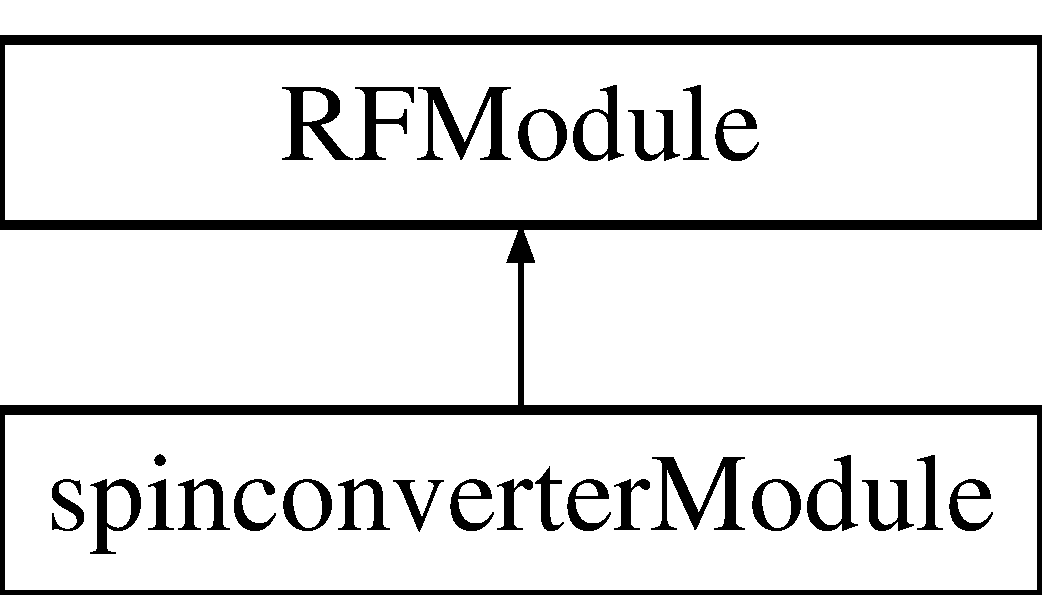
\includegraphics[height=2.000000cm]{classspinconverterModule}
\end{center}
\end{figure}
\subsection*{Public Member Functions}
\begin{DoxyCompactItemize}
\item 
virtual bool {\bfseries configure} (yarp\+::os\+::\+Resource\+Finder \&rf)\hypertarget{classspinconverterModule_ac0b34ed884eb17bd4a6f52c8b3630a2c}{}\label{classspinconverterModule_ac0b34ed884eb17bd4a6f52c8b3630a2c}

\item 
virtual bool {\bfseries interrupt\+Module} ()\hypertarget{classspinconverterModule_a9893addfd6adc708ceccddc4c3e9183a}{}\label{classspinconverterModule_a9893addfd6adc708ceccddc4c3e9183a}

\item 
virtual bool {\bfseries close} ()\hypertarget{classspinconverterModule_acb2fc1926feaa32b83b9eeb4cd031b25}{}\label{classspinconverterModule_acb2fc1926feaa32b83b9eeb4cd031b25}

\item 
virtual bool {\bfseries respond} (const yarp\+::os\+::\+Bottle \&command, yarp\+::os\+::\+Bottle \&reply)\hypertarget{classspinconverterModule_a22d21aab95bd5e24501bae68ae3a5921}{}\label{classspinconverterModule_a22d21aab95bd5e24501bae68ae3a5921}

\item 
virtual double {\bfseries get\+Period} ()\hypertarget{classspinconverterModule_a8a9564ee39fec8095257846d7eb43ca6}{}\label{classspinconverterModule_a8a9564ee39fec8095257846d7eb43ca6}

\item 
virtual bool {\bfseries update\+Module} ()\hypertarget{classspinconverterModule_abc54e110dbae422e61b21de1d12f9fc0}{}\label{classspinconverterModule_abc54e110dbae422e61b21de1d12f9fc0}

\end{DoxyCompactItemize}


The documentation for this class was generated from the following files\+:\begin{DoxyCompactItemize}
\item 
/home/aglover/workspace/projects/event-\/driven/src/modules/spinconverter/include/spinconverter.\+h\item 
/home/aglover/workspace/projects/event-\/driven/src/modules/spinconverter/src/spinconverter.\+cpp\end{DoxyCompactItemize}

\hypertarget{classev_1_1temporalSurface}{}\section{ev\+:\+:temporal\+Surface Class Reference}
\label{classev_1_1temporalSurface}\index{ev\+::temporal\+Surface@{ev\+::temporal\+Surface}}
Inheritance diagram for ev\+:\+:temporal\+Surface\+:\begin{figure}[H]
\begin{center}
\leavevmode
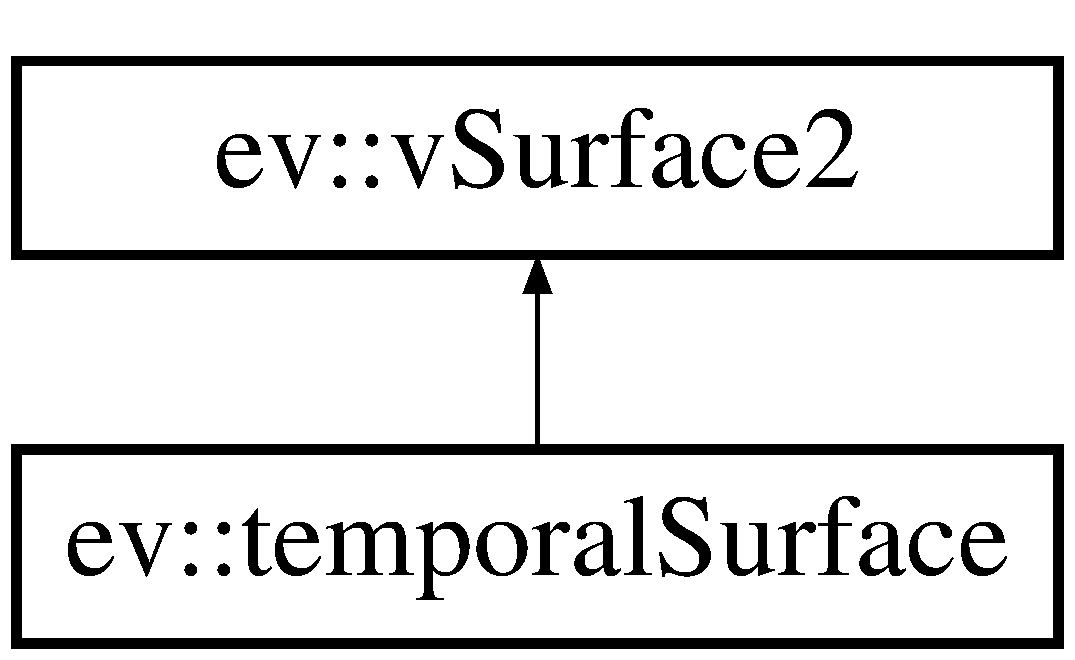
\includegraphics[height=2.000000cm]{classev_1_1temporalSurface}
\end{center}
\end{figure}
\subsection*{Public Member Functions}
\begin{DoxyCompactItemize}
\item 
{\bfseries temporal\+Surface} (int \hyperlink{classev_1_1vSurface2_a1aa8027816352a15d5b9bf1f26f48e76}{width}=128, int height=128, int duration=vts\+Helper\+::max\+Stamp()$\ast$0.\+5)\hypertarget{classev_1_1temporalSurface_ad2f8ebcbe5ff5825d0473cd05f00389e}{}\label{classev_1_1temporalSurface_ad2f8ebcbe5ff5825d0473cd05f00389e}

\item 
virtual \hyperlink{classev_1_1vQueue}{v\+Queue} {\bfseries remove\+Events} (event$<$$>$ to\+Add)\hypertarget{classev_1_1temporalSurface_a358c548e6727aa89d908e61ad948b1ca}{}\label{classev_1_1temporalSurface_a358c548e6727aa89d908e61ad948b1ca}

\item 
void {\bfseries set\+Temporal\+Size} (int duration)\hypertarget{classev_1_1temporalSurface_a35d4b67c18393961fa833d330a040e80}{}\label{classev_1_1temporalSurface_a35d4b67c18393961fa833d330a040e80}

\end{DoxyCompactItemize}
\subsection*{Additional Inherited Members}


The documentation for this class was generated from the following files\+:\begin{DoxyCompactItemize}
\item 
/home/aglover/workspace/projects/event-\/driven/libraries/include/i\+Cub/eventdriven/v\+Window.\+h\item 
/home/aglover/workspace/projects/event-\/driven/libraries/src/v\+Window.\+cpp\end{DoxyCompactItemize}

\hypertarget{classTrackerPool}{}\section{Tracker\+Pool Class Reference}
\label{classTrackerPool}\index{Tracker\+Pool@{Tracker\+Pool}}
\subsection*{Public Member Functions}
\begin{DoxyCompactItemize}
\item 
void {\bfseries set\+Initial\+Params} (double sig\+\_\+x, double sig\+\_\+y, double sig\+\_\+xy, double alpha\+\_\+pos, double alpha\+\_\+shape, bool fixed\+\_\+shape)\hypertarget{classTrackerPool_aba64099a18fc9b97eeb5b60f92ca849c}{}\label{classTrackerPool_aba64099a18fc9b97eeb5b60f92ca849c}

\item 
void {\bfseries set\+Decay\+Params} (double decay\+\_\+tau, double Tact, double Tinact, double Tfree, double Tevent, int rate)\hypertarget{classTrackerPool_aacfd7b8d8f8d47cf609e6e4ed64bbc1a}{}\label{classTrackerPool_aacfd7b8d8f8d47cf609e6e4ed64bbc1a}

\item 
void {\bfseries set\+Comparison\+Params} (double max\+\_\+dist)\hypertarget{classTrackerPool_a2ae5849c22bc24b688bd5ddf153e9e33}{}\label{classTrackerPool_a2ae5849c22bc24b688bd5ddf153e9e33}

\item 
void {\bfseries set\+Cluster\+Limit} (int limit)\hypertarget{classTrackerPool_a947f58bef9d46a290cb3ea6ec99d5fb8}{}\label{classTrackerPool_a947f58bef9d46a290cb3ea6ec99d5fb8}

\item 
int {\bfseries update} (ev\+::event$<$ \hyperlink{classev_1_1AddressEvent}{ev\+::\+Address\+Event} $>$ v, std\+::vector$<$ ev\+::event$<$ \hyperlink{classev_1_1ClusterEventGauss}{ev\+::\+Cluster\+Event\+Gauss} $>$ $>$ \&cl\+Evts)\hypertarget{classTrackerPool_ae64eee2fd11a6e3402cc94b12480b97a}{}\label{classTrackerPool_ae64eee2fd11a6e3402cc94b12480b97a}

\end{DoxyCompactItemize}
\subsection*{Protected Member Functions}
\begin{DoxyCompactItemize}
\item 
int {\bfseries get\+New\+Tracker} ()\hypertarget{classTrackerPool_afc17f68023420c6d43ac4b67afa3b14d}{}\label{classTrackerPool_afc17f68023420c6d43ac4b67afa3b14d}

\item 
ev\+::event$<$ \hyperlink{classev_1_1ClusterEventGauss}{ev\+::\+Cluster\+Event\+Gauss} $>$ {\bfseries make\+Event} (int i, int ts)\hypertarget{classTrackerPool_ab180f70f6ab8d8315ab38c37fed4507b}{}\label{classTrackerPool_ab180f70f6ab8d8315ab38c37fed4507b}

\end{DoxyCompactItemize}
\subsection*{Protected Attributes}
\begin{DoxyCompactItemize}
\item 
std\+::vector$<$ \hyperlink{classBlobTracker}{Blob\+Tracker} $>$ {\bfseries trackers\+\_\+}\hypertarget{classTrackerPool_a8a8bdb245a4e706de8f9263cc31537cd}{}\label{classTrackerPool_a8a8bdb245a4e706de8f9263cc31537cd}

\item 
int {\bfseries nb\+\_\+ev\+\_\+regulate\+\_\+}\hypertarget{classTrackerPool_af542ddb16630e451065d5e3258cd19de}{}\label{classTrackerPool_af542ddb16630e451065d5e3258cd19de}

\item 
int {\bfseries count\+\_\+}\hypertarget{classTrackerPool_a5aed0a9c9621c9fde35034a8b5f58085}{}\label{classTrackerPool_a5aed0a9c9621c9fde35034a8b5f58085}

\item 
unsigned long int {\bfseries ts\+\_\+last\+\_\+reg\+\_\+}\hypertarget{classTrackerPool_ac8ecd306ab6f0562ca2d6231ff367093}{}\label{classTrackerPool_ac8ecd306ab6f0562ca2d6231ff367093}

\item 
double {\bfseries decay\+\_\+tau}\hypertarget{classTrackerPool_abe7439ab3a403e77b56def1ae14ef1c3}{}\label{classTrackerPool_abe7439ab3a403e77b56def1ae14ef1c3}

\item 
double {\bfseries Tact}\hypertarget{classTrackerPool_aaf7de0a0903e66d7ae07cc11cb6ea072}{}\label{classTrackerPool_aaf7de0a0903e66d7ae07cc11cb6ea072}

\item 
double {\bfseries Tinact}\hypertarget{classTrackerPool_a75d2a1d3867ac839d3c24aa26241950e}{}\label{classTrackerPool_a75d2a1d3867ac839d3c24aa26241950e}

\item 
double {\bfseries Tfree}\hypertarget{classTrackerPool_ac75f2360d9bb76e0a6c79b31129c58c5}{}\label{classTrackerPool_ac75f2360d9bb76e0a6c79b31129c58c5}

\item 
double {\bfseries Tevent}\hypertarget{classTrackerPool_a3798b118a9592e75d59ad0d0e5fe438b}{}\label{classTrackerPool_a3798b118a9592e75d59ad0d0e5fe438b}

\item 
double {\bfseries max\+\_\+dist}\hypertarget{classTrackerPool_ad57d26c00d4329747f59df1b7b24ea3b}{}\label{classTrackerPool_ad57d26c00d4329747f59df1b7b24ea3b}

\item 
bool {\bfseries fixed\+\_\+shape\+\_\+}\hypertarget{classTrackerPool_af83ad39640f58a747253b85046083140}{}\label{classTrackerPool_af83ad39640f58a747253b85046083140}

\item 
double {\bfseries sig\+\_\+x2\+\_\+}\hypertarget{classTrackerPool_a6a92ea09387253159839324143b6206a}{}\label{classTrackerPool_a6a92ea09387253159839324143b6206a}

\item 
double {\bfseries sig\+\_\+y2\+\_\+}\hypertarget{classTrackerPool_a3181cb8343949ab80181c9028ae114fa}{}\label{classTrackerPool_a3181cb8343949ab80181c9028ae114fa}

\item 
double {\bfseries sig\+\_\+xy\+\_\+}\hypertarget{classTrackerPool_a9018c85457b2616efe8f718f1602b32a}{}\label{classTrackerPool_a9018c85457b2616efe8f718f1602b32a}

\item 
double {\bfseries alpha\+\_\+pos}\hypertarget{classTrackerPool_ad67aaae3b2c777330ccb4abb9bf60884}{}\label{classTrackerPool_ad67aaae3b2c777330ccb4abb9bf60884}

\item 
double {\bfseries alpha\+\_\+shape}\hypertarget{classTrackerPool_ad134dda445a2b5eea2d2101a6e5c2132}{}\label{classTrackerPool_ad134dda445a2b5eea2d2101a6e5c2132}

\item 
double {\bfseries cluster\+Limit}\hypertarget{classTrackerPool_a6c9e6cdff31c0ab40c19f54d30d315cc}{}\label{classTrackerPool_a6c9e6cdff31c0ab40c19f54d30d315cc}

\item 
\hyperlink{classev_1_1vtsHelper}{ev\+::vts\+Helper} {\bfseries unwrap}\hypertarget{classTrackerPool_afec5b627c70b35454cecd812b3913c59}{}\label{classTrackerPool_afec5b627c70b35454cecd812b3913c59}

\end{DoxyCompactItemize}


The documentation for this class was generated from the following files\+:\begin{DoxyCompactItemize}
\item 
/home/aglover/workspace/projects/event-\/driven/src/modules/v\+Cluster/include/tracker\+Pool.\+h\item 
/home/aglover/workspace/projects/event-\/driven/src/modules/v\+Cluster/src/tracker\+Pool.\+cpp\end{DoxyCompactItemize}

\hypertarget{classev_1_1vBottle}{}\section{ev\+:\+:v\+Bottle Class Reference}
\label{classev_1_1vBottle}\index{ev\+::v\+Bottle@{ev\+::v\+Bottle}}
Inheritance diagram for ev\+:\+:v\+Bottle\+:\begin{figure}[H]
\begin{center}
\leavevmode
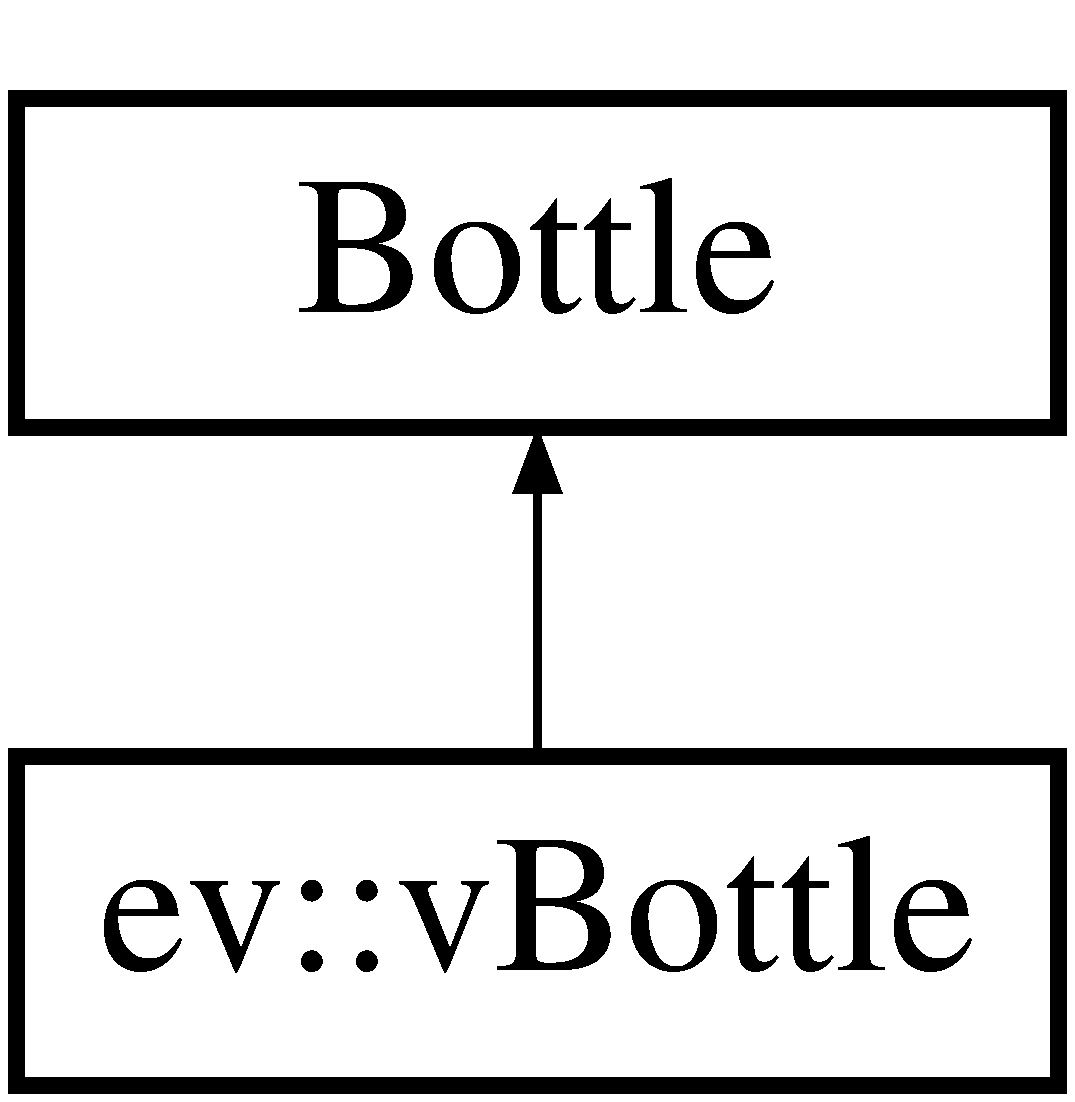
\includegraphics[height=2.000000cm]{classev_1_1vBottle}
\end{center}
\end{figure}
\subsection*{Public Member Functions}
\begin{DoxyCompactItemize}
\item 
void {\bfseries add\+Event} (event$<$$>$ e)\hypertarget{classev_1_1vBottle_a5b17f0b46d9260ab255f38382b4b7268}{}\label{classev_1_1vBottle_a5b17f0b46d9260ab255f38382b4b7268}

\item 
void {\bfseries append} (\hyperlink{classev_1_1vBottle}{v\+Bottle} \&eb)\hypertarget{classev_1_1vBottle_a0c78e6f9ef839038d71486f6a8a6294a}{}\label{classev_1_1vBottle_a0c78e6f9ef839038d71486f6a8a6294a}

\item 
{\footnotesize template$<$class T $>$ }\\void {\bfseries append} (\hyperlink{classev_1_1vBottle}{v\+Bottle} \&eb)\hypertarget{classev_1_1vBottle_a9ef66f613e1bbf196c515e7d8b0416df}{}\label{classev_1_1vBottle_a9ef66f613e1bbf196c515e7d8b0416df}

\item 
{\footnotesize template$<$class T $>$ }\\\hyperlink{classev_1_1vQueue}{v\+Queue} {\bfseries get} ()\hypertarget{classev_1_1vBottle_a86302277c279a1b02d92f8e12afe6a2c}{}\label{classev_1_1vBottle_a86302277c279a1b02d92f8e12afe6a2c}

\item 
{\footnotesize template$<$class T $>$ }\\void {\bfseries addtoendof} (\hyperlink{classev_1_1vQueue}{v\+Queue} \&q)\hypertarget{classev_1_1vBottle_a65bf90aec03b80dee45bf834efe3fbfc}{}\label{classev_1_1vBottle_a65bf90aec03b80dee45bf834efe3fbfc}

\item 
{\footnotesize template$<$class T $>$ }\\\hyperlink{classev_1_1vQueue}{v\+Queue} {\bfseries get\+Sorted} ()\hypertarget{classev_1_1vBottle_a27569b9aaa7eb1ff9135d435b841c2de}{}\label{classev_1_1vBottle_a27569b9aaa7eb1ff9135d435b841c2de}

\item 
\hyperlink{classev_1_1vQueue}{v\+Queue} {\bfseries get\+All} ()\hypertarget{classev_1_1vBottle_af2abadf41f73c455dd451e34e9ba3376}{}\label{classev_1_1vBottle_af2abadf41f73c455dd451e34e9ba3376}

\item 
\hyperlink{classev_1_1vQueue}{v\+Queue} {\bfseries get\+All\+Sorted} ()\hypertarget{classev_1_1vBottle_a273cfda65fed58bcf19cedf6652948d9}{}\label{classev_1_1vBottle_a273cfda65fed58bcf19cedf6652948d9}

\end{DoxyCompactItemize}


The documentation for this class was generated from the following file\+:\begin{DoxyCompactItemize}
\item 
/home/aglover/workspace/projects/event-\/driven/libraries/include/i\+Cub/eventdriven/v\+Bottle.\+h\end{DoxyCompactItemize}

\hypertarget{classev_1_1vBottleMimic}{}\section{ev\+:\+:v\+Bottle\+Mimic Class Reference}
\label{classev_1_1vBottleMimic}\index{ev\+::v\+Bottle\+Mimic@{ev\+::v\+Bottle\+Mimic}}
Inheritance diagram for ev\+:\+:v\+Bottle\+Mimic\+:\begin{figure}[H]
\begin{center}
\leavevmode
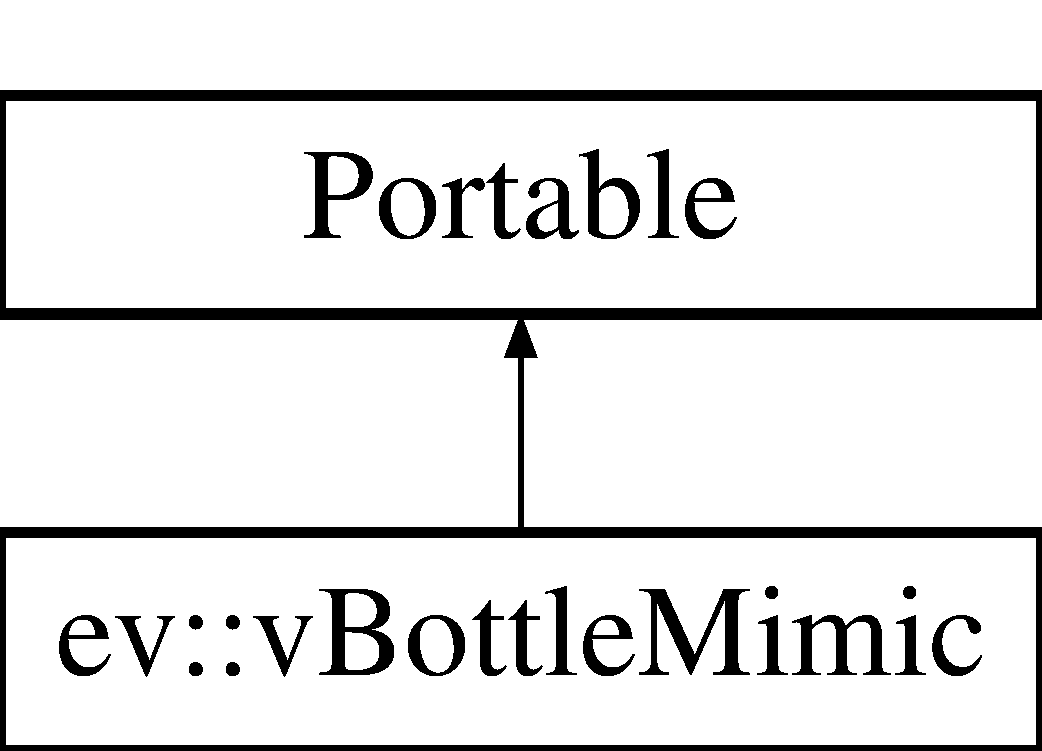
\includegraphics[height=2.000000cm]{classev_1_1vBottleMimic}
\end{center}
\end{figure}
\subsection*{Public Member Functions}
\begin{DoxyCompactItemize}
\item 
void {\bfseries setdata} (const char $\ast$datablock, unsigned int datalength)\hypertarget{classev_1_1vBottleMimic_a03c64a63225e333a11b2693213f44165}{}\label{classev_1_1vBottleMimic_a03c64a63225e333a11b2693213f44165}

\item 
virtual bool {\bfseries read} (yarp\+::os\+::\+Connection\+Reader \&connection)\hypertarget{classev_1_1vBottleMimic_a5c7ead7b0484b9abe99e922196c074ff}{}\label{classev_1_1vBottleMimic_a5c7ead7b0484b9abe99e922196c074ff}

\item 
virtual bool {\bfseries write} (yarp\+::os\+::\+Connection\+Writer \&connection)\hypertarget{classev_1_1vBottleMimic_a39ad9b924890d8f8f717f49b6c5ad23f}{}\label{classev_1_1vBottleMimic_a39ad9b924890d8f8f717f49b6c5ad23f}

\end{DoxyCompactItemize}


The documentation for this class was generated from the following file\+:\begin{DoxyCompactItemize}
\item 
/home/aglover/workspace/projects/event-\/driven/libraries/include/i\+Cub/eventdriven/v\+Bottle.\+h\end{DoxyCompactItemize}

\hypertarget{classvcdModule}{}\section{vcd\+Module Class Reference}
\label{classvcdModule}\index{vcd\+Module@{vcd\+Module}}
Inheritance diagram for vcd\+Module\+:\begin{figure}[H]
\begin{center}
\leavevmode
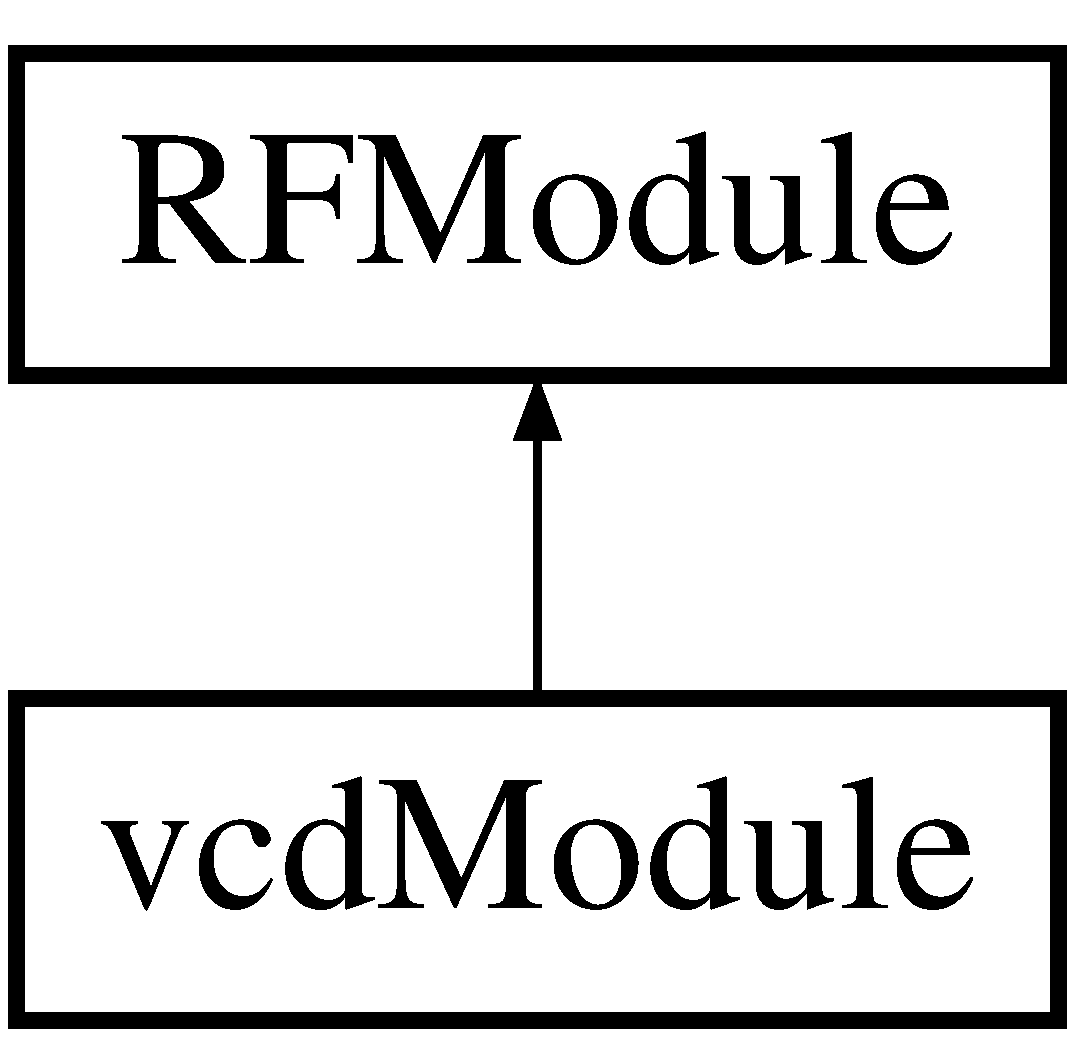
\includegraphics[height=2.000000cm]{classvcdModule}
\end{center}
\end{figure}
\subsection*{Public Member Functions}
\begin{DoxyCompactItemize}
\item 
virtual bool {\bfseries configure} (yarp\+::os\+::\+Resource\+Finder \&rf)\hypertarget{classvcdModule_a72f6523b85d300a2a8aceb82501e05f7}{}\label{classvcdModule_a72f6523b85d300a2a8aceb82501e05f7}

\item 
virtual bool {\bfseries interrupt\+Module} ()\hypertarget{classvcdModule_a73bd29efc30b548bc4935b2d56089fd3}{}\label{classvcdModule_a73bd29efc30b548bc4935b2d56089fd3}

\item 
virtual bool {\bfseries close} ()\hypertarget{classvcdModule_ad92e877a36ac7e9548bf7dcad67575ae}{}\label{classvcdModule_ad92e877a36ac7e9548bf7dcad67575ae}

\item 
virtual double {\bfseries get\+Period} ()\hypertarget{classvcdModule_ac8c7b1f48ecd3022cd7b19fe1d9466e6}{}\label{classvcdModule_ac8c7b1f48ecd3022cd7b19fe1d9466e6}

\item 
virtual bool {\bfseries update\+Module} ()\hypertarget{classvcdModule_a493580c216623260104f0e13749031b0}{}\label{classvcdModule_a493580c216623260104f0e13749031b0}

\end{DoxyCompactItemize}


The documentation for this class was generated from the following files\+:\begin{DoxyCompactItemize}
\item 
/home/aglover/workspace/projects/event-\/driven/src/modules/v\+Circle\+Disparity/include/v\+Circle\+Disparity.\+h\item 
/home/aglover/workspace/projects/event-\/driven/src/modules/v\+Circle\+Disparity/src/v\+Circle\+Disparity.\+cpp\end{DoxyCompactItemize}

\hypertarget{classvCircleModule}{}\section{v\+Circle\+Module Class Reference}
\label{classvCircleModule}\index{v\+Circle\+Module@{v\+Circle\+Module}}
Inheritance diagram for v\+Circle\+Module\+:\begin{figure}[H]
\begin{center}
\leavevmode
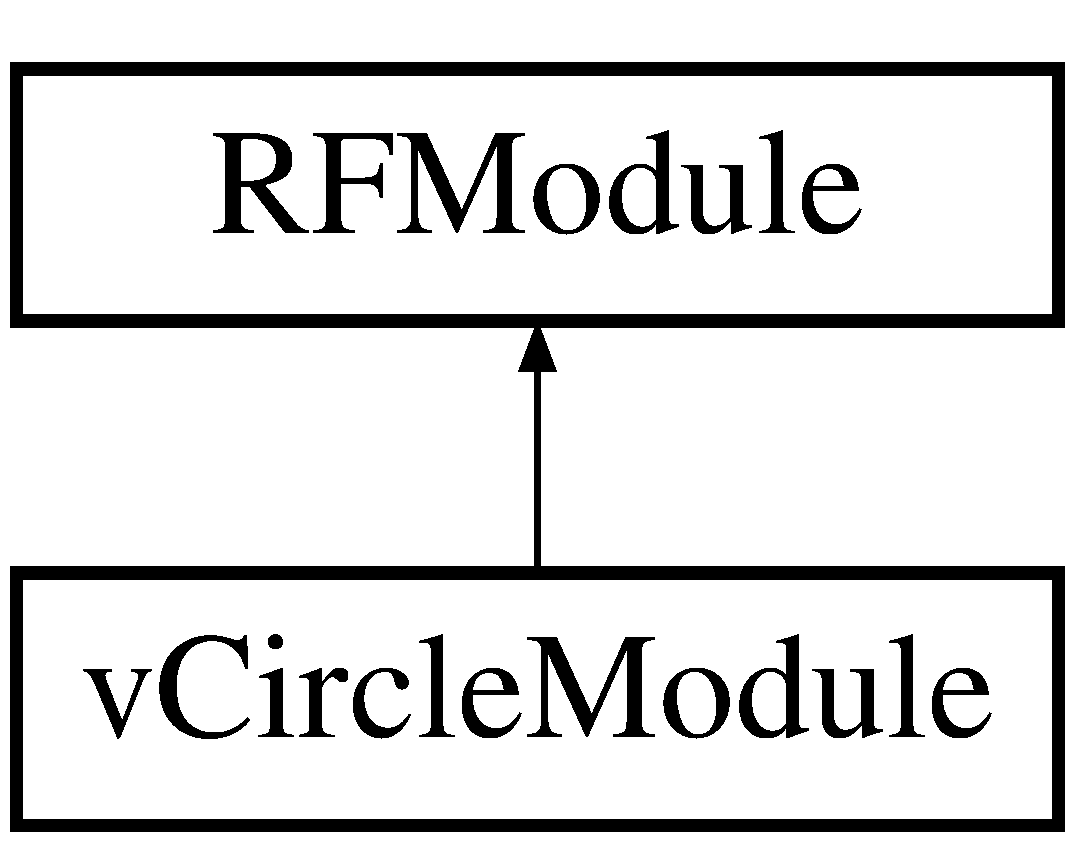
\includegraphics[height=2.000000cm]{classvCircleModule}
\end{center}
\end{figure}
\subsection*{Public Member Functions}
\begin{DoxyCompactItemize}
\item 
virtual bool {\bfseries configure} (yarp\+::os\+::\+Resource\+Finder \&rf)\hypertarget{classvCircleModule_a4b1534c8acd2a20a874b1e3fb2f2bbbf}{}\label{classvCircleModule_a4b1534c8acd2a20a874b1e3fb2f2bbbf}

\item 
virtual bool {\bfseries interrupt\+Module} ()\hypertarget{classvCircleModule_aee48b945926e1ee1d53c03d2f8fdb462}{}\label{classvCircleModule_aee48b945926e1ee1d53c03d2f8fdb462}

\item 
virtual bool {\bfseries close} ()\hypertarget{classvCircleModule_a9c266baf21bf1a84e1d47bc82a6ebbaa}{}\label{classvCircleModule_a9c266baf21bf1a84e1d47bc82a6ebbaa}

\item 
virtual double {\bfseries get\+Period} ()\hypertarget{classvCircleModule_a87f95035935e336eef6b9890920c1bcb}{}\label{classvCircleModule_a87f95035935e336eef6b9890920c1bcb}

\item 
virtual bool {\bfseries update\+Module} ()\hypertarget{classvCircleModule_a0137387e1760f41bb422e10c702df2a0}{}\label{classvCircleModule_a0137387e1760f41bb422e10c702df2a0}

\end{DoxyCompactItemize}


The documentation for this class was generated from the following files\+:\begin{DoxyCompactItemize}
\item 
/home/aglover/workspace/projects/event-\/driven/src/modules/v\+Circle/include/v\+Circle\+Module.\+h\item 
/home/aglover/workspace/projects/event-\/driven/src/modules/v\+Circle/src/v\+Circle\+Module.\+cpp\end{DoxyCompactItemize}

\hypertarget{classvCircleMultiSize}{}\section{v\+Circle\+Multi\+Size Class Reference}
\label{classvCircleMultiSize}\index{v\+Circle\+Multi\+Size@{v\+Circle\+Multi\+Size}}
\subsection*{Public Member Functions}
\begin{DoxyCompactItemize}
\item 
{\bfseries v\+Circle\+Multi\+Size} (double threshold, std\+::string q\+Type=\char`\"{}edge\char`\"{}, int r\+Low=8, int r\+High=38, bool directed=true, bool parallel=false, int height=128, int width=128, int arclength=20, double fifolength=2000)\hypertarget{classvCircleMultiSize_aa3e7373ef68728fab536417c491e35a4}{}\label{classvCircleMultiSize_aa3e7373ef68728fab536417c491e35a4}

\item 
void {\bfseries set\+Channel} (int channel\+Number)\hypertarget{classvCircleMultiSize_afe4c5983834ed7d5fa097fcc9677d234}{}\label{classvCircleMultiSize_afe4c5983834ed7d5fa097fcc9677d234}

\item 
void {\bfseries add\+Queue} (\hyperlink{classev_1_1vQueue}{ev\+::v\+Queue} \&additions)\hypertarget{classvCircleMultiSize_a101a1960c5012a83e03b9fdd8276f263}{}\label{classvCircleMultiSize_a101a1960c5012a83e03b9fdd8276f263}

\item 
double {\bfseries get\+Obs} (int \&x, int \&y, int \&r)\hypertarget{classvCircleMultiSize_a661f425152259951f87167bdcd53caaf}{}\label{classvCircleMultiSize_a661f425152259951f87167bdcd53caaf}

\item 
std\+::vector$<$ double $>$ {\bfseries get\+Percentile} (double p, double th\+Min)\hypertarget{classvCircleMultiSize_a92b94e14acce928e07922809a45cd5c0}{}\label{classvCircleMultiSize_a92b94e14acce928e07922809a45cd5c0}

\item 
yarp\+::sig\+::\+Image\+Of$<$ yarp\+::sig\+::\+Pixel\+Bgr $>$ {\bfseries make\+Debug\+Image} ()\hypertarget{classvCircleMultiSize_a1dc2c81da6abc8aaaaedf0d169ad9671}{}\label{classvCircleMultiSize_a1dc2c81da6abc8aaaaedf0d169ad9671}

\end{DoxyCompactItemize}


The documentation for this class was generated from the following files\+:\begin{DoxyCompactItemize}
\item 
/home/aglover/workspace/projects/event-\/driven/src/modules/v\+Circle/include/v\+Circle\+Observer.\+h\item 
/home/aglover/workspace/projects/event-\/driven/src/modules/v\+Circle/src/v\+Circle\+Observer.\+cpp\end{DoxyCompactItemize}

\hypertarget{classvCircleReader}{}\section{v\+Circle\+Reader Class Reference}
\label{classvCircleReader}\index{v\+Circle\+Reader@{v\+Circle\+Reader}}
Inheritance diagram for v\+Circle\+Reader\+:\begin{figure}[H]
\begin{center}
\leavevmode
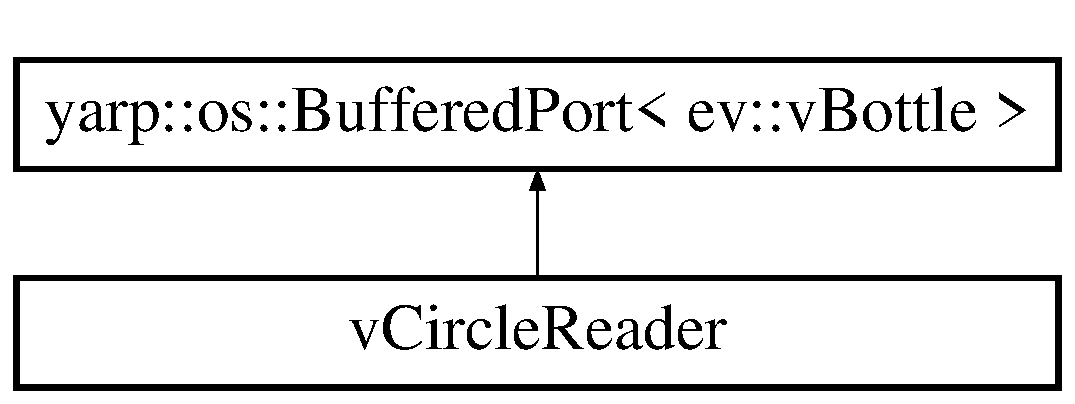
\includegraphics[height=2.000000cm]{classvCircleReader}
\end{center}
\end{figure}
\subsection*{Public Member Functions}
\begin{DoxyCompactItemize}
\item 
void {\bfseries set\+SingleQ} (bool singleq=true)\hypertarget{classvCircleReader_a35b57eb759bf78b3199e2b058f509b19}{}\label{classvCircleReader_a35b57eb759bf78b3199e2b058f509b19}

\item 
bool {\bfseries open} (const std\+::string \&name, bool strictness=false)\hypertarget{classvCircleReader_aeea09b1b0a4f6ca43362430e2b7c13f3}{}\label{classvCircleReader_aeea09b1b0a4f6ca43362430e2b7c13f3}

\item 
void {\bfseries close} ()\hypertarget{classvCircleReader_a963ecb3d9e66c9a6d0dd3deb0107d333}{}\label{classvCircleReader_a963ecb3d9e66c9a6d0dd3deb0107d333}

\item 
void {\bfseries interrupt} ()\hypertarget{classvCircleReader_adb1e49808d1ff24b38e68ad3c706d87a}{}\label{classvCircleReader_adb1e49808d1ff24b38e68ad3c706d87a}

\item 
void {\bfseries on\+Read} (\hyperlink{classev_1_1vBottle}{ev\+::v\+Bottle} \&in\+Bot)\hypertarget{classvCircleReader_ae0f761bdd9af2bae8edc2e0f2766ff39}{}\label{classvCircleReader_ae0f761bdd9af2bae8edc2e0f2766ff39}

\end{DoxyCompactItemize}
\subsection*{Public Attributes}
\begin{DoxyCompactItemize}
\item 
\hyperlink{classvCircleTracker}{v\+Circle\+Tracker} {\bfseries circle\+Tracker}\hypertarget{classvCircleReader_a7b0ae9557cbe36e72339cc7479d99833}{}\label{classvCircleReader_a7b0ae9557cbe36e72339cc7479d99833}

\item 
\hyperlink{classvCircleMultiSize}{v\+Circle\+Multi\+Size} $\ast$ {\bfseries c\+ObserverL}\hypertarget{classvCircleReader_a75c47ee3024729fab391fc0098147430}{}\label{classvCircleReader_a75c47ee3024729fab391fc0098147430}

\item 
\hyperlink{classvCircleMultiSize}{v\+Circle\+Multi\+Size} $\ast$ {\bfseries c\+ObserverR}\hypertarget{classvCircleReader_a52940184b5d5f348813fdfdf1a62da48}{}\label{classvCircleReader_a52940184b5d5f348813fdfdf1a62da48}

\item 
double {\bfseries inlier\+Threshold}\hypertarget{classvCircleReader_abb1da4c345eb519b695927d12f2f1ec8}{}\label{classvCircleReader_abb1da4c345eb519b695927d12f2f1ec8}

\item 
bool {\bfseries hough}\hypertarget{classvCircleReader_a2a026b4c43ab7e721b6089b4118767a4}{}\label{classvCircleReader_a2a026b4c43ab7e721b6089b4118767a4}

\item 
double {\bfseries timecounter}\hypertarget{classvCircleReader_a0bcf9e8b5c28b2ea048ab75c4213023e}{}\label{classvCircleReader_a0bcf9e8b5c28b2ea048ab75c4213023e}

\end{DoxyCompactItemize}


The documentation for this class was generated from the following files\+:\begin{DoxyCompactItemize}
\item 
/home/aglover/workspace/projects/event-\/driven/src/modules/v\+Circle/include/v\+Circle\+Module.\+h\item 
/home/aglover/workspace/projects/event-\/driven/src/modules/v\+Circle/src/v\+Circle\+Module.\+cpp\end{DoxyCompactItemize}

\hypertarget{classvCircleThread}{}\section{v\+Circle\+Thread Class Reference}
\label{classvCircleThread}\index{v\+Circle\+Thread@{v\+Circle\+Thread}}


The \hyperlink{classvCircleThread}{v\+Circle\+Thread} class performs a circular Hough transform.  




{\ttfamily \#include $<$v\+Circle\+Observer.\+h$>$}

Inheritance diagram for v\+Circle\+Thread\+:\begin{figure}[H]
\begin{center}
\leavevmode
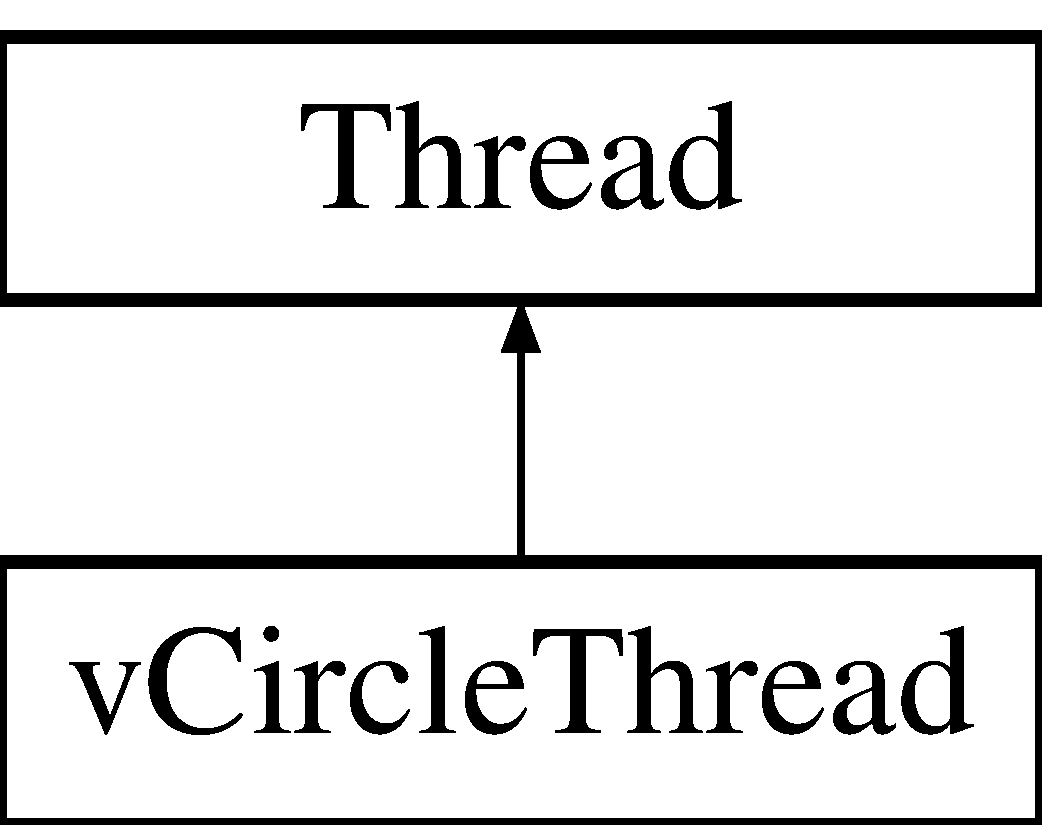
\includegraphics[height=2.000000cm]{classvCircleThread}
\end{center}
\end{figure}
\subsection*{Public Member Functions}
\begin{DoxyCompactItemize}
\item 
\hyperlink{classvCircleThread_adb0ce9432b9fe2a8d853c63b764d7859}{v\+Circle\+Thread} (int R, bool directed, bool parallel=false, int height=128, int width=128, double arclength=15)
\begin{DoxyCompactList}\small\item\em \hyperlink{classvCircleThread}{v\+Circle\+Thread} constructor \end{DoxyCompactList}\item 
double \hyperlink{classvCircleThread_a692a1066ee63c2716998fcb3a7aa513d}{get\+Score} ()
\begin{DoxyCompactList}\small\item\em get\+Score get the maximum strength in Hough space \end{DoxyCompactList}\item 
int \hyperlink{classvCircleThread_a0feac9f937bfeecc2dc0b015f9e8161c}{getX} ()
\begin{DoxyCompactList}\small\item\em getX get the maximum strength location \end{DoxyCompactList}\item 
int \hyperlink{classvCircleThread_a4f39898c53c3178b84b28c8cc33ec352}{getY} ()
\begin{DoxyCompactList}\small\item\em getY get the maximum strength location \end{DoxyCompactList}\item 
int \hyperlink{classvCircleThread_a024aa1ad0a7855fad146425c80feadb0}{getR} ()
\begin{DoxyCompactList}\small\item\em getR return the radius of the circle to be detected \end{DoxyCompactList}\item 
void \hyperlink{classvCircleThread_ad5f114e5609dd616c9eae9d1755d12c1}{process} (\hyperlink{classev_1_1vQueue}{ev\+::v\+Queue} \&proc\+Queue, std\+::vector$<$ int $>$ \&proc\+Type)
\begin{DoxyCompactList}\small\item\em process update the Hough transform (threaded or non-\/threaded) \end{DoxyCompactList}\item 
void \hyperlink{classvCircleThread_a0d32749f12d2d93ff0d9ccdf37422ccf}{waitfordone} ()\hypertarget{classvCircleThread_a0d32749f12d2d93ff0d9ccdf37422ccf}{}\label{classvCircleThread_a0d32749f12d2d93ff0d9ccdf37422ccf}

\begin{DoxyCompactList}\small\item\em waitfordone wait for computation to finish if threaded \end{DoxyCompactList}\item 
int {\bfseries find\+Scores} (std\+::vector$<$ double $>$ \&values, double threshold)\hypertarget{classvCircleThread_a89b389603f6f6a9395a0381271dee419}{}\label{classvCircleThread_a89b389603f6f6a9395a0381271dee419}

\item 
yarp\+::sig\+::\+Image\+Of$<$ yarp\+::sig\+::\+Pixel\+Bgr $>$ \hyperlink{classvCircleThread_ae19a982e66ba27619a40ecbf128af543}{make\+Debug\+Image} (double refval=-\/1)
\begin{DoxyCompactList}\small\item\em make\+Debug\+Image create an image visualising the Hough space \end{DoxyCompactList}\end{DoxyCompactItemize}


\subsection{Detailed Description}
The \hyperlink{classvCircleThread}{v\+Circle\+Thread} class performs a circular Hough transform. 

The class gives the maximal location and strength of a circular shape of a single given radius. The class can use the directed transform and can be threaded for use on multi-\/core systems. 

\subsection{Constructor \& Destructor Documentation}
\index{v\+Circle\+Thread@{v\+Circle\+Thread}!v\+Circle\+Thread@{v\+Circle\+Thread}}
\index{v\+Circle\+Thread@{v\+Circle\+Thread}!v\+Circle\+Thread@{v\+Circle\+Thread}}
\subsubsection[{\texorpdfstring{v\+Circle\+Thread(int R, bool directed, bool parallel=false, int height=128, int width=128, double arclength=15)}{vCircleThread(int R, bool directed, bool parallel=false, int height=128, int width=128, double arclength=15)}}]{\setlength{\rightskip}{0pt plus 5cm}v\+Circle\+Thread\+::v\+Circle\+Thread (
\begin{DoxyParamCaption}
\item[{int}]{R, }
\item[{bool}]{directed, }
\item[{bool}]{parallel = {\ttfamily false}, }
\item[{int}]{height = {\ttfamily 128}, }
\item[{int}]{width = {\ttfamily 128}, }
\item[{double}]{arclength = {\ttfamily 15}}
\end{DoxyParamCaption}
)}\hypertarget{classvCircleThread_adb0ce9432b9fe2a8d853c63b764d7859}{}\label{classvCircleThread_adb0ce9432b9fe2a8d853c63b764d7859}


\hyperlink{classvCircleThread}{v\+Circle\+Thread} constructor 


\begin{DoxyParams}{Parameters}
{\em R} & circle radius \\
\hline
{\em directed} & use directed Hough transform \\
\hline
{\em parallel} & use a separate thread for computation \\
\hline
{\em height} & sensor height \\
\hline
{\em width} & sensor width \\
\hline
\end{DoxyParams}


\subsection{Member Function Documentation}
\index{v\+Circle\+Thread@{v\+Circle\+Thread}!getR@{getR}}
\index{getR@{getR}!v\+Circle\+Thread@{v\+Circle\+Thread}}
\subsubsection[{\texorpdfstring{get\+R()}{getR()}}]{\setlength{\rightskip}{0pt plus 5cm}int v\+Circle\+Thread\+::getR (
\begin{DoxyParamCaption}
{}
\end{DoxyParamCaption}
)\hspace{0.3cm}{\ttfamily [inline]}}\hypertarget{classvCircleThread_a024aa1ad0a7855fad146425c80feadb0}{}\label{classvCircleThread_a024aa1ad0a7855fad146425c80feadb0}


getR return the radius of the circle to be detected 

\begin{DoxyReturn}{Returns}
the radius R 
\end{DoxyReturn}
\index{v\+Circle\+Thread@{v\+Circle\+Thread}!get\+Score@{get\+Score}}
\index{get\+Score@{get\+Score}!v\+Circle\+Thread@{v\+Circle\+Thread}}
\subsubsection[{\texorpdfstring{get\+Score()}{getScore()}}]{\setlength{\rightskip}{0pt plus 5cm}double v\+Circle\+Thread\+::get\+Score (
\begin{DoxyParamCaption}
{}
\end{DoxyParamCaption}
)\hspace{0.3cm}{\ttfamily [inline]}}\hypertarget{classvCircleThread_a692a1066ee63c2716998fcb3a7aa513d}{}\label{classvCircleThread_a692a1066ee63c2716998fcb3a7aa513d}


get\+Score get the maximum strength in Hough space 

\begin{DoxyReturn}{Returns}
the maximum strength in Hough space 
\end{DoxyReturn}
\index{v\+Circle\+Thread@{v\+Circle\+Thread}!getX@{getX}}
\index{getX@{getX}!v\+Circle\+Thread@{v\+Circle\+Thread}}
\subsubsection[{\texorpdfstring{get\+X()}{getX()}}]{\setlength{\rightskip}{0pt plus 5cm}int v\+Circle\+Thread\+::getX (
\begin{DoxyParamCaption}
{}
\end{DoxyParamCaption}
)\hspace{0.3cm}{\ttfamily [inline]}}\hypertarget{classvCircleThread_a0feac9f937bfeecc2dc0b015f9e8161c}{}\label{classvCircleThread_a0feac9f937bfeecc2dc0b015f9e8161c}


getX get the maximum strength location 

\begin{DoxyReturn}{Returns}
maximum strength location along x axis 
\end{DoxyReturn}
\index{v\+Circle\+Thread@{v\+Circle\+Thread}!getY@{getY}}
\index{getY@{getY}!v\+Circle\+Thread@{v\+Circle\+Thread}}
\subsubsection[{\texorpdfstring{get\+Y()}{getY()}}]{\setlength{\rightskip}{0pt plus 5cm}int v\+Circle\+Thread\+::getY (
\begin{DoxyParamCaption}
{}
\end{DoxyParamCaption}
)\hspace{0.3cm}{\ttfamily [inline]}}\hypertarget{classvCircleThread_a4f39898c53c3178b84b28c8cc33ec352}{}\label{classvCircleThread_a4f39898c53c3178b84b28c8cc33ec352}


getY get the maximum strength location 

\begin{DoxyReturn}{Returns}
maximum strength location along y axis 
\end{DoxyReturn}
\index{v\+Circle\+Thread@{v\+Circle\+Thread}!make\+Debug\+Image@{make\+Debug\+Image}}
\index{make\+Debug\+Image@{make\+Debug\+Image}!v\+Circle\+Thread@{v\+Circle\+Thread}}
\subsubsection[{\texorpdfstring{make\+Debug\+Image(double refval=-\/1)}{makeDebugImage(double refval=-1)}}]{\setlength{\rightskip}{0pt plus 5cm}yarp\+::sig\+::\+Image\+Of$<$ yarp\+::sig\+::\+Pixel\+Bgr $>$ v\+Circle\+Thread\+::make\+Debug\+Image (
\begin{DoxyParamCaption}
\item[{double}]{refval = {\ttfamily -\/1}}
\end{DoxyParamCaption}
)}\hypertarget{classvCircleThread_ae19a982e66ba27619a40ecbf128af543}{}\label{classvCircleThread_ae19a982e66ba27619a40ecbf128af543}


make\+Debug\+Image create an image visualising the Hough space 

\begin{DoxyReturn}{Returns}
a B\+GR yarp image 
\end{DoxyReturn}
\index{v\+Circle\+Thread@{v\+Circle\+Thread}!process@{process}}
\index{process@{process}!v\+Circle\+Thread@{v\+Circle\+Thread}}
\subsubsection[{\texorpdfstring{process(ev\+::v\+Queue \&proc\+Queue, std\+::vector$<$ int $>$ \&proc\+Type)}{process(ev::vQueue &procQueue, std::vector< int > &procType)}}]{\setlength{\rightskip}{0pt plus 5cm}void v\+Circle\+Thread\+::process (
\begin{DoxyParamCaption}
\item[{{\bf ev\+::v\+Queue} \&}]{proc\+Queue, }
\item[{std\+::vector$<$ int $>$ \&}]{proc\+Type}
\end{DoxyParamCaption}
)}\hypertarget{classvCircleThread_ad5f114e5609dd616c9eae9d1755d12c1}{}\label{classvCircleThread_ad5f114e5609dd616c9eae9d1755d12c1}


process update the Hough transform (threaded or non-\/threaded) 


\begin{DoxyParams}{Parameters}
{\em adds} & list of events to add \\
\hline
{\em subs} & list of events to remove \\
\hline
\end{DoxyParams}


The documentation for this class was generated from the following files\+:\begin{DoxyCompactItemize}
\item 
/home/aglover/workspace/projects/event-\/driven/src/modules/v\+Circle/include/v\+Circle\+Observer.\+h\item 
/home/aglover/workspace/projects/event-\/driven/src/modules/v\+Circle/src/v\+Circle\+Observer.\+cpp\end{DoxyCompactItemize}

\hypertarget{classvCircleTracker}{}\section{v\+Circle\+Tracker Class Reference}
\label{classvCircleTracker}\index{v\+Circle\+Tracker@{v\+Circle\+Tracker}}
\subsection*{Public Member Functions}
\begin{DoxyCompactItemize}
\item 
void {\bfseries init} (double sv\+Pos, double sv\+Siz, double zv\+Pos, double zv\+Siz)\hypertarget{classvCircleTracker_af2b25d915f5c517b64514409fb993703}{}\label{classvCircleTracker_af2b25d915f5c517b64514409fb993703}

\item 
bool {\bfseries start\+Tracking} (double xz, double yz, double rz)\hypertarget{classvCircleTracker_aab8929299dc8caf0393d4c1565a05995}{}\label{classvCircleTracker_aab8929299dc8caf0393d4c1565a05995}

\item 
double {\bfseries predict} (double dt)\hypertarget{classvCircleTracker_ae56bc313864551e5f8b09dedebec0d79}{}\label{classvCircleTracker_ae56bc313864551e5f8b09dedebec0d79}

\item 
bool {\bfseries correct} (double xz, double yz, double rz)\hypertarget{classvCircleTracker_ad84e5c23fec79d12f1f5007176d4fe4f}{}\label{classvCircleTracker_ad84e5c23fec79d12f1f5007176d4fe4f}

\item 
bool {\bfseries get\+State} (double \&x, double \&y, double \&r)\hypertarget{classvCircleTracker_a41cfcda05d1e9e46bf98636c045cc326}{}\label{classvCircleTracker_a41cfcda05d1e9e46bf98636c045cc326}

\item 
double {\bfseries Pzgd} (double xz, double yz, double rz)\hypertarget{classvCircleTracker_ad1d7602e56934c432c46aaeb639a5015}{}\label{classvCircleTracker_ad1d7602e56934c432c46aaeb639a5015}

\item 
bool {\bfseries is\+Active} ()\hypertarget{classvCircleTracker_a99d43513683806249f7bdc36a8879b4f}{}\label{classvCircleTracker_a99d43513683806249f7bdc36a8879b4f}

\end{DoxyCompactItemize}


The documentation for this class was generated from the following files\+:\begin{DoxyCompactItemize}
\item 
/home/aglover/workspace/projects/event-\/driven/src/modules/v\+Circle/include/v\+Circle\+Track.\+h\item 
/home/aglover/workspace/projects/event-\/driven/src/modules/v\+Circle/src/v\+Circle\+Track.\+cpp\end{DoxyCompactItemize}

\hypertarget{classvCornerManager}{}\section{v\+Corner\+Manager Class Reference}
\label{classvCornerManager}\index{v\+Corner\+Manager@{v\+Corner\+Manager}}
Inheritance diagram for v\+Corner\+Manager\+:\begin{figure}[H]
\begin{center}
\leavevmode
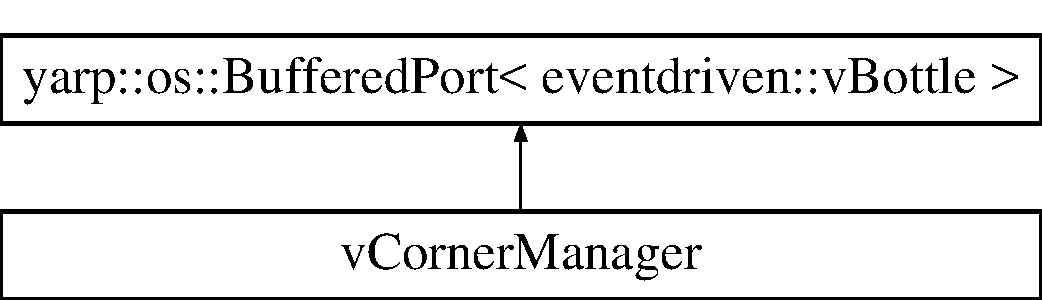
\includegraphics[height=2.000000cm]{classvCornerManager}
\end{center}
\end{figure}
\subsection*{Public Member Functions}
\begin{DoxyCompactItemize}
\item 
{\bfseries v\+Corner\+Manager} (int height, int width, int filter\+Size, int thickness, double thresh)\hypertarget{classvCornerManager_a767e4a3bac4f9c20da2da54eef8a12f3}{}\label{classvCornerManager_a767e4a3bac4f9c20da2da54eef8a12f3}

\item 
bool {\bfseries open} (const std\+::string module\+Name, bool strictness=false)\hypertarget{classvCornerManager_ae87a3b35a1047404536af869dd837621}{}\label{classvCornerManager_ae87a3b35a1047404536af869dd837621}

\item 
void {\bfseries close} ()\hypertarget{classvCornerManager_acf1440f33d67878234673e9d4d65a5bf}{}\label{classvCornerManager_acf1440f33d67878234673e9d4d65a5bf}

\item 
void {\bfseries interrupt} ()\hypertarget{classvCornerManager_a360ad86c3e051d7f452bdb4c8d82b28d}{}\label{classvCornerManager_a360ad86c3e051d7f452bdb4c8d82b28d}

\item 
void {\bfseries on\+Read} (eventdriven\+::v\+Bottle \&bot)\hypertarget{classvCornerManager_aa7d750d2fbc1b09ff705ec5b27018cee}{}\label{classvCornerManager_aa7d750d2fbc1b09ff705ec5b27018cee}

\end{DoxyCompactItemize}


The documentation for this class was generated from the following files\+:\begin{DoxyCompactItemize}
\item 
/home/aglover/workspace/projects/event-\/driven/src/modules/v\+Corner/include/v\+Corner.\+h\item 
/home/aglover/workspace/projects/event-\/driven/src/modules/v\+Corner/src/v\+Corner.\+cpp\end{DoxyCompactItemize}

\hypertarget{classvCornerModule}{}\section{v\+Corner\+Module Class Reference}
\label{classvCornerModule}\index{v\+Corner\+Module@{v\+Corner\+Module}}
Inheritance diagram for v\+Corner\+Module\+:\begin{figure}[H]
\begin{center}
\leavevmode
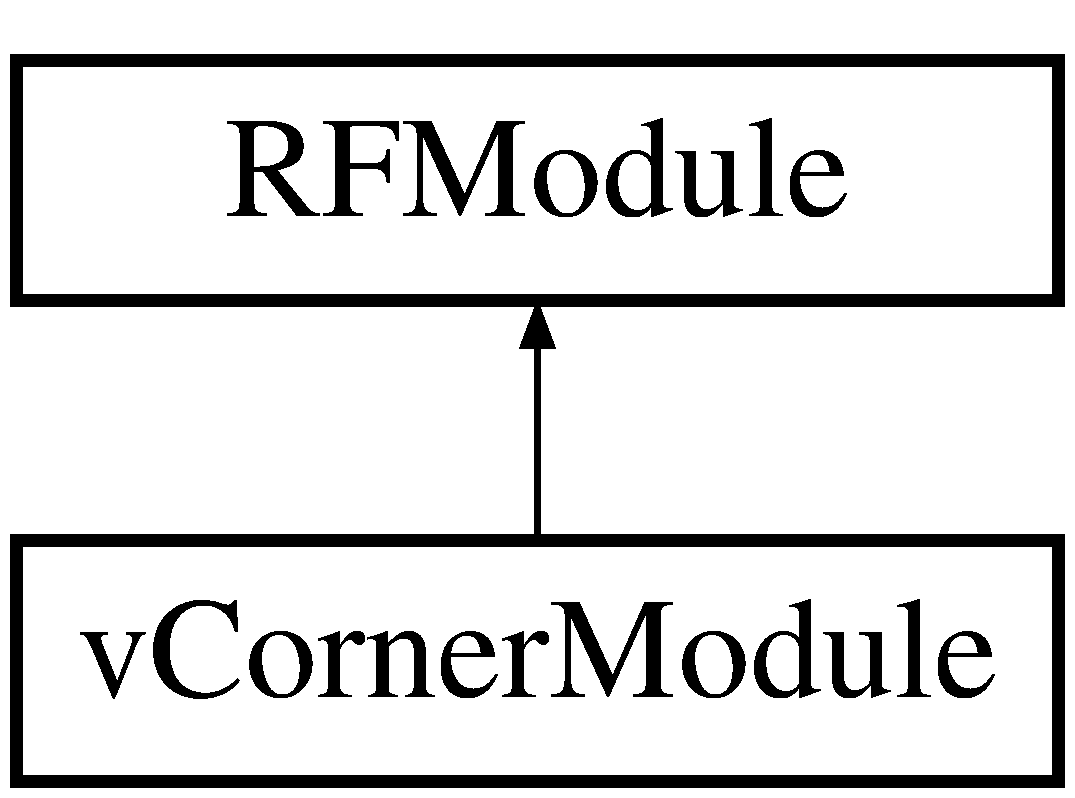
\includegraphics[height=2.000000cm]{classvCornerModule}
\end{center}
\end{figure}
\subsection*{Public Member Functions}
\begin{DoxyCompactItemize}
\item 
virtual bool {\bfseries configure} (yarp\+::os\+::\+Resource\+Finder \&rf)\hypertarget{classvCornerModule_a9496d5d39d6b65dc048ce147ed2856d8}{}\label{classvCornerModule_a9496d5d39d6b65dc048ce147ed2856d8}

\item 
virtual bool {\bfseries interrupt\+Module} ()\hypertarget{classvCornerModule_a8354934bd0d851418e99d93c567f5020}{}\label{classvCornerModule_a8354934bd0d851418e99d93c567f5020}

\item 
virtual bool {\bfseries close} ()\hypertarget{classvCornerModule_aa66707b60e2f920a5faff5c13798b785}{}\label{classvCornerModule_aa66707b60e2f920a5faff5c13798b785}

\item 
virtual double {\bfseries get\+Period} ()\hypertarget{classvCornerModule_afc071a27e74fe3ab6d23a78b25844df4}{}\label{classvCornerModule_afc071a27e74fe3ab6d23a78b25844df4}

\item 
virtual bool {\bfseries update\+Module} ()\hypertarget{classvCornerModule_af25a4ba8a2b8346f0a3a69b6e80998c8}{}\label{classvCornerModule_af25a4ba8a2b8346f0a3a69b6e80998c8}

\end{DoxyCompactItemize}


The documentation for this class was generated from the following files\+:\begin{DoxyCompactItemize}
\item 
/home/aglover/workspace/projects/event-\/driven/src/modules/v\+Corner/include/v\+Corner.\+h\item 
/home/aglover/workspace/projects/event-\/driven/src/modules/v\+Corner/src/v\+Corner.\+cpp\end{DoxyCompactItemize}

\hypertarget{classvDevCtrl}{}\section{v\+Dev\+Ctrl Class Reference}
\label{classvDevCtrl}\index{v\+Dev\+Ctrl@{v\+Dev\+Ctrl}}
\subsection*{Public Member Functions}
\begin{DoxyCompactItemize}
\item 
{\bfseries v\+Dev\+Ctrl} (std\+::string device\+Name=\char`\"{}\char`\"{}, unsigned char i2c\+Address=0)\hypertarget{classvDevCtrl_a28270bc81b8f37400562730649b9ea20}{}\label{classvDevCtrl_a28270bc81b8f37400562730649b9ea20}

\item 
bool {\bfseries set\+Bias} (std\+::string bias\+Name, unsigned int bias\+Value)\hypertarget{classvDevCtrl_ad7c8b642dc056c3e0475af546ed6e534}{}\label{classvDevCtrl_ad7c8b642dc056c3e0475af546ed6e534}

\item 
bool {\bfseries set\+Bias} (yarp\+::os\+::\+Bottle bias)\hypertarget{classvDevCtrl_ac95a8bc8aedcd40fa1fa8089e568390b}{}\label{classvDevCtrl_ac95a8bc8aedcd40fa1fa8089e568390b}

\item 
unsigned int {\bfseries get\+Bias} (std\+::string bias\+Name)\hypertarget{classvDevCtrl_a37baee231dd38b573c674fca0ac0024e}{}\label{classvDevCtrl_a37baee231dd38b573c674fca0ac0024e}

\item 
bool {\bfseries connect} (void)\hypertarget{classvDevCtrl_af6ccda24918a78cd5eb800c3f11c07c4}{}\label{classvDevCtrl_af6ccda24918a78cd5eb800c3f11c07c4}

\item 
bool {\bfseries configure} (bool verbose=false)\hypertarget{classvDevCtrl_a432d0c5cb40afbce3e14a685cfdd11c0}{}\label{classvDevCtrl_a432d0c5cb40afbce3e14a685cfdd11c0}

\item 
void {\bfseries disconnect} (bool andturnoff=true)\hypertarget{classvDevCtrl_a274051caa72b84acac607ebb3d7ec2e2}{}\label{classvDevCtrl_a274051caa72b84acac607ebb3d7ec2e2}

\item 
bool {\bfseries activate} (bool active=true)\hypertarget{classvDevCtrl_a737b66cec44fc2bd0ebb29dccf15838b}{}\label{classvDevCtrl_a737b66cec44fc2bd0ebb29dccf15838b}

\item 
bool {\bfseries suspend} (void)\hypertarget{classvDevCtrl_a9cc8b11acf775f7c7afaf736ffe69c52}{}\label{classvDevCtrl_a9cc8b11acf775f7c7afaf736ffe69c52}

\item 
bool {\bfseries configure\+Biases} ()\hypertarget{classvDevCtrl_a33fb7c392cfdaad5c35b7683eacc61e2}{}\label{classvDevCtrl_a33fb7c392cfdaad5c35b7683eacc61e2}

\item 
void {\bfseries print\+Configuration} (void)\hypertarget{classvDevCtrl_a4fc72bb26da523c7c731b9465e19a5cd}{}\label{classvDevCtrl_a4fc72bb26da523c7c731b9465e19a5cd}

\end{DoxyCompactItemize}


The documentation for this class was generated from the following files\+:\begin{DoxyCompactItemize}
\item 
/home/aglover/workspace/projects/event-\/driven/src/hardwareio/zynq\+Grabber/include/device\+Controller.\+h\item 
/home/aglover/workspace/projects/event-\/driven/src/hardwareio/zynq\+Grabber/src/device\+Controller.\+cpp\end{DoxyCompactItemize}

\hypertarget{classvDevReadBuffer}{}\section{v\+Dev\+Read\+Buffer Class Reference}
\label{classvDevReadBuffer}\index{v\+Dev\+Read\+Buffer@{v\+Dev\+Read\+Buffer}}
Inheritance diagram for v\+Dev\+Read\+Buffer\+:\begin{figure}[H]
\begin{center}
\leavevmode
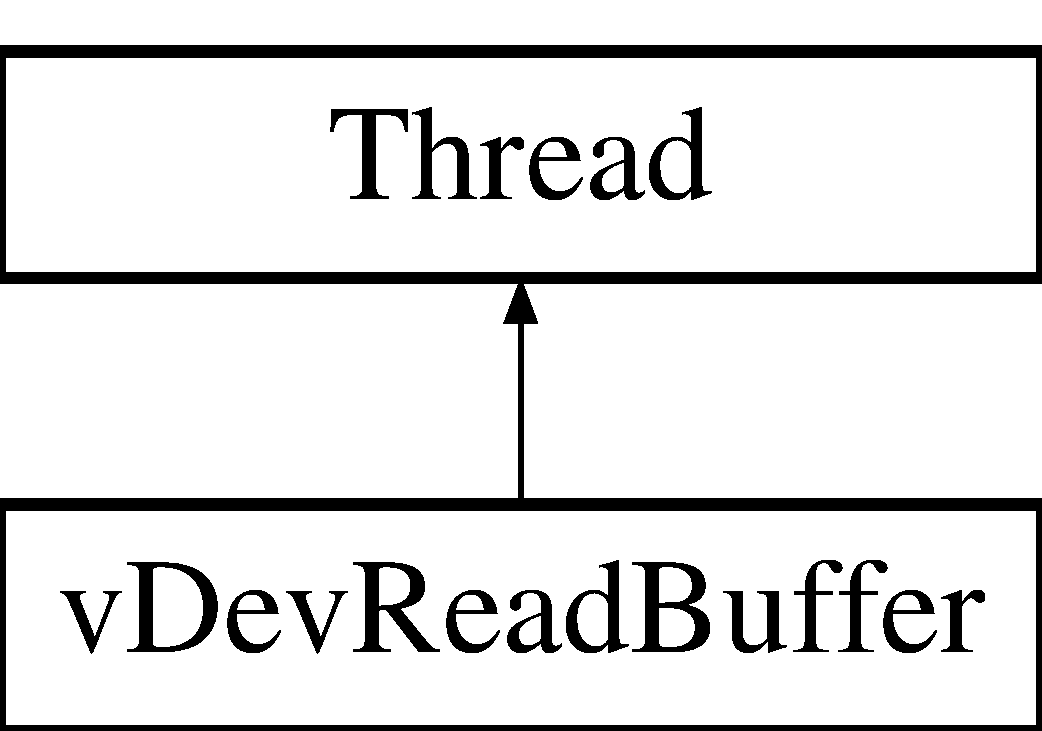
\includegraphics[height=2.000000cm]{classvDevReadBuffer}
\end{center}
\end{figure}
\subsection*{Public Member Functions}
\begin{DoxyCompactItemize}
\item 
bool {\bfseries initialise} (std\+::string devicename, unsigned int buffer\+Size=0, unsigned int read\+Size=0)\hypertarget{classvDevReadBuffer_aed2023a30193768d35ffc3684c826142}{}\label{classvDevReadBuffer_aed2023a30193768d35ffc3684c826142}

\item 
virtual void {\bfseries run} ()\hypertarget{classvDevReadBuffer_a8d3e3995a073efe42d6a8693b66cf87e}{}\label{classvDevReadBuffer_a8d3e3995a073efe42d6a8693b66cf87e}

\item 
virtual void {\bfseries thread\+Release} ()\hypertarget{classvDevReadBuffer_a763f76c090da36846824bbe5a3365278}{}\label{classvDevReadBuffer_a763f76c090da36846824bbe5a3365278}

\item 
std\+::vector$<$ unsigned char $>$ \& {\bfseries get\+Buffer} (unsigned int \&n\+Bytes\+Read, unsigned int \&n\+Bytes\+Lost)\hypertarget{classvDevReadBuffer_a8fd5cc78799d0b9ddcacd958a84c316e}{}\label{classvDevReadBuffer_a8fd5cc78799d0b9ddcacd958a84c316e}

\end{DoxyCompactItemize}


The documentation for this class was generated from the following files\+:\begin{DoxyCompactItemize}
\item 
/home/aglover/workspace/projects/event-\/driven/src/hardwareio/zynq\+Grabber/include/yarp\+Interface.\+h\item 
/home/aglover/workspace/projects/event-\/driven/src/hardwareio/zynq\+Grabber/src/yarp\+Interface.\+cpp\end{DoxyCompactItemize}

\hypertarget{classev_1_1vEdge}{}\section{ev\+:\+:v\+Edge Class Reference}
\label{classev_1_1vEdge}\index{ev\+::v\+Edge@{ev\+::v\+Edge}}
Inheritance diagram for ev\+:\+:v\+Edge\+:\begin{figure}[H]
\begin{center}
\leavevmode
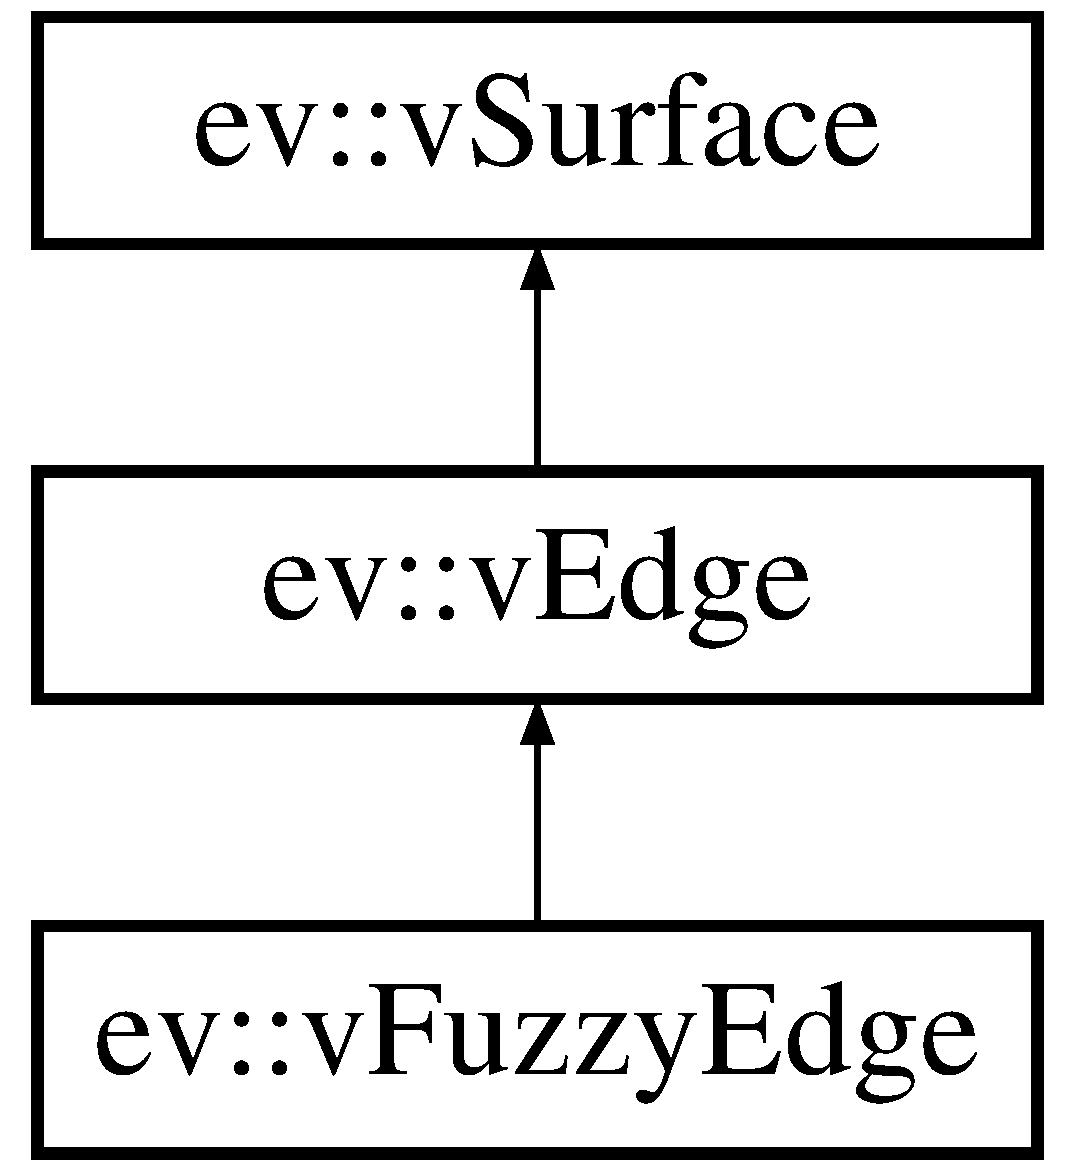
\includegraphics[height=3.000000cm]{classev_1_1vEdge}
\end{center}
\end{figure}
\subsection*{Public Member Functions}
\begin{DoxyCompactItemize}
\item 
{\bfseries v\+Edge} (int \hyperlink{classev_1_1vSurface_a9666b7ae2580bf5647f65306f911825e}{width}=128, int \hyperlink{classev_1_1vSurface_ab3cf3df2f4fcb7eb5d89e0c5d1a5eeff}{height}=128)\hypertarget{classev_1_1vEdge_a3bbccb1784adbb0543a22e6e1a805be5}{}\label{classev_1_1vEdge_a3bbccb1784adbb0543a22e6e1a805be5}

\item 
\hyperlink{classev_1_1vQueue}{v\+Queue} {\bfseries add\+Event\+To\+Edge} (event$<$ \hyperlink{classev_1_1AddressEvent}{Address\+Event} $>$ v)\hypertarget{classev_1_1vEdge_a04bc02981fe09b9cc0615a471a4d1594}{}\label{classev_1_1vEdge_a04bc02981fe09b9cc0615a471a4d1594}

\item 
void {\bfseries set\+Thickness} (int pixels)\hypertarget{classev_1_1vEdge_a8add033e36c36c4145d932d8e210750a}{}\label{classev_1_1vEdge_a8add033e36c36c4145d932d8e210750a}

\item 
void {\bfseries track} (bool track\+Count=true)\hypertarget{classev_1_1vEdge_a7e0dd1c7f362d79a0cef3298caa74f8a}{}\label{classev_1_1vEdge_a7e0dd1c7f362d79a0cef3298caa74f8a}

\item 
virtual const \hyperlink{classev_1_1vQueue}{v\+Queue} \& {\bfseries get\+Surf} (int xl, int xh, int yl, int yh)\hypertarget{classev_1_1vEdge_a87ffb2ce22e33ff630703dfd8cb24f8e}{}\label{classev_1_1vEdge_a87ffb2ce22e33ff630703dfd8cb24f8e}

\end{DoxyCompactItemize}
\subsection*{Additional Inherited Members}


The documentation for this class was generated from the following files\+:\begin{DoxyCompactItemize}
\item 
/home/aglover/workspace/projects/event-\/driven/libraries/include/i\+Cub/eventdriven/v\+Surface.\+h\item 
/home/aglover/workspace/projects/event-\/driven/libraries/src/v\+Surface.\+cpp\end{DoxyCompactItemize}

\hypertarget{classev_1_1vEvent}{}\section{ev\+:\+:v\+Event Class Reference}
\label{classev_1_1vEvent}\index{ev\+::v\+Event@{ev\+::v\+Event}}
Inheritance diagram for ev\+:\+:v\+Event\+:\begin{figure}[H]
\begin{center}
\leavevmode
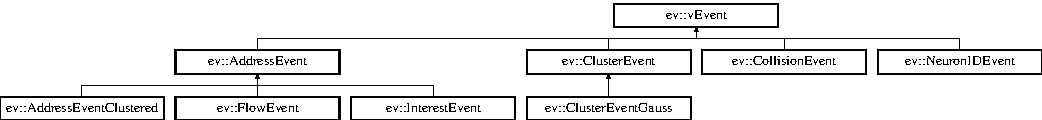
\includegraphics[height=1.618497cm]{classev_1_1vEvent}
\end{center}
\end{figure}
\subsection*{Public Member Functions}
\begin{DoxyCompactItemize}
\item 
\hyperlink{classev_1_1vEvent_a397825b956ef6d60cbedaa27414117bc}{v\+Event} ()\hypertarget{classev_1_1vEvent_a397825b956ef6d60cbedaa27414117bc}{}\label{classev_1_1vEvent_a397825b956ef6d60cbedaa27414117bc}

\begin{DoxyCompactList}\small\item\em blank constructor required at base level \end{DoxyCompactList}\item 
\hyperlink{classev_1_1vEvent_aaba2a98a5821fbad33523f558e9c565a}{v\+Event} (const \hyperlink{classev_1_1vEvent}{v\+Event} \&event)\hypertarget{classev_1_1vEvent_aaba2a98a5821fbad33523f558e9c565a}{}\label{classev_1_1vEvent_aaba2a98a5821fbad33523f558e9c565a}

\begin{DoxyCompactList}\small\item\em copy constructor \end{DoxyCompactList}\item 
virtual std\+::string {\bfseries get\+Type} () const \hypertarget{classev_1_1vEvent_a78ae84b6bc48e188a48803c0a63c7eec}{}\label{classev_1_1vEvent_a78ae84b6bc48e188a48803c0a63c7eec}

\item 
void {\bfseries set\+Stamp} (const unsigned int stamp)\hypertarget{classev_1_1vEvent_a23a27198e491e78b2dd90261d272c3a3}{}\label{classev_1_1vEvent_a23a27198e491e78b2dd90261d272c3a3}

\item 
int {\bfseries get\+Stamp} () const \hypertarget{classev_1_1vEvent_a8f24ece8c78e3b657228359643c9afbf}{}\label{classev_1_1vEvent_a8f24ece8c78e3b657228359643c9afbf}

\item 
virtual int {\bfseries get\+Channel} () const \hypertarget{classev_1_1vEvent_a195be4c62f8464a3bb8101d74ca3aabd}{}\label{classev_1_1vEvent_a195be4c62f8464a3bb8101d74ca3aabd}

\item 
virtual int {\bfseries get\+Polarity} () const \hypertarget{classev_1_1vEvent_a36d189c20a3fab42021de214a64ff5ee}{}\label{classev_1_1vEvent_a36d189c20a3fab42021de214a64ff5ee}

\item 
virtual \hyperlink{classev_1_1vEvent}{v\+Event} \& {\bfseries operator=} (const \hyperlink{classev_1_1vEvent}{v\+Event} \&event)\hypertarget{classev_1_1vEvent_a26f0b1283811c19e46ad859c00c651ce}{}\label{classev_1_1vEvent_a26f0b1283811c19e46ad859c00c651ce}

\item 
virtual bool {\bfseries operator==} (const \hyperlink{classev_1_1vEvent}{v\+Event} \&event)\hypertarget{classev_1_1vEvent_a294910360dc519411aad9c6162e2bece}{}\label{classev_1_1vEvent_a294910360dc519411aad9c6162e2bece}

\item 
virtual bool {\bfseries operator$<$} (const \hyperlink{classev_1_1vEvent}{v\+Event} \&event) const \hypertarget{classev_1_1vEvent_aed871fc1325a013061219459843d2b73}{}\label{classev_1_1vEvent_aed871fc1325a013061219459843d2b73}

\item 
virtual bool {\bfseries operator$>$} (const \hyperlink{classev_1_1vEvent}{v\+Event} \&event) const \hypertarget{classev_1_1vEvent_a5e6c2c5499df00db97c707c17dc00c67}{}\label{classev_1_1vEvent_a5e6c2c5499df00db97c707c17dc00c67}

\item 
virtual \hyperlink{classev_1_1vEvent}{v\+Event} $\ast$ {\bfseries clone} ()\hypertarget{classev_1_1vEvent_a1ec88aa748ba04cda2ff146067c77b7b}{}\label{classev_1_1vEvent_a1ec88aa748ba04cda2ff146067c77b7b}

\item 
virtual void {\bfseries encode} (yarp\+::os\+::\+Bottle \&b) const \hypertarget{classev_1_1vEvent_a66d9e4d833031c146cc0ac3af332b1cc}{}\label{classev_1_1vEvent_a66d9e4d833031c146cc0ac3af332b1cc}

\item 
virtual bool {\bfseries decode} (const yarp\+::os\+::\+Bottle \&packet, int \&pos)\hypertarget{classev_1_1vEvent_a75132601bf3f958212fd3793b7e53139}{}\label{classev_1_1vEvent_a75132601bf3f958212fd3793b7e53139}

\item 
virtual yarp\+::os\+::\+Property {\bfseries get\+Content} () const \hypertarget{classev_1_1vEvent_adabb906a71f96c89d6d539c899044622}{}\label{classev_1_1vEvent_adabb906a71f96c89d6d539c899044622}

\item 
virtual int {\bfseries n\+Bytes\+Coded} () const \hypertarget{classev_1_1vEvent_ad962c635597189c17957f3d73e64346d}{}\label{classev_1_1vEvent_ad962c635597189c17957f3d73e64346d}

\end{DoxyCompactItemize}
\subsection*{Protected Attributes}
\begin{DoxyCompactItemize}
\item 
unsigned int {\bfseries stamp}\+:24\hypertarget{classev_1_1vEvent_ad4e003653fa59b37682addefce835490}{}\label{classev_1_1vEvent_ad4e003653fa59b37682addefce835490}

\end{DoxyCompactItemize}


The documentation for this class was generated from the following files\+:\begin{DoxyCompactItemize}
\item 
/home/aglover/workspace/projects/event-\/driven/libraries/include/i\+Cub/eventdriven/v\+Codec.\+h\item 
/home/aglover/workspace/projects/event-\/driven/libraries/src/v\+Codec.\+cpp\end{DoxyCompactItemize}

\hypertarget{classvFlowManager}{}\section{v\+Flow\+Manager Class Reference}
\label{classvFlowManager}\index{v\+Flow\+Manager@{v\+Flow\+Manager}}
Inheritance diagram for v\+Flow\+Manager\+:\begin{figure}[H]
\begin{center}
\leavevmode
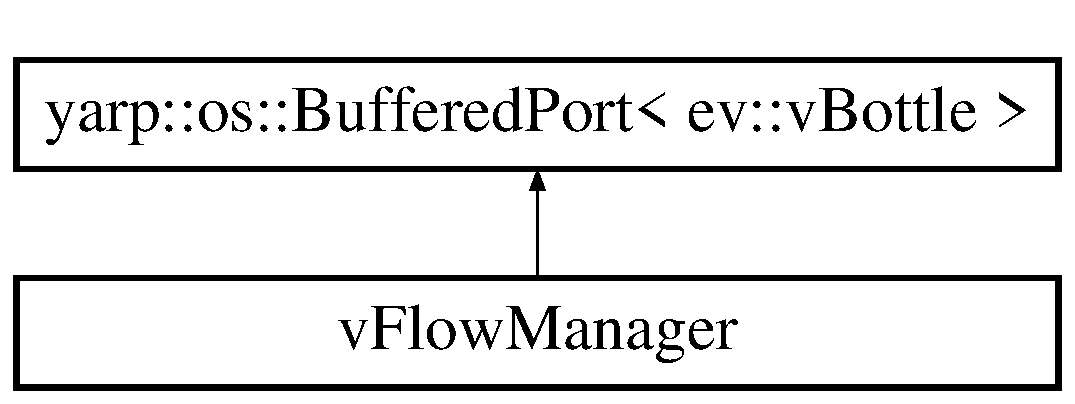
\includegraphics[height=2.000000cm]{classvFlowManager}
\end{center}
\end{figure}
\subsection*{Public Member Functions}
\begin{DoxyCompactItemize}
\item 
{\bfseries v\+Flow\+Manager} (int height, int width, int filter\+Size, int min\+Evts\+On\+Plane)\hypertarget{classvFlowManager_a9d28c98ce6f6c0591a89f5055153e295}{}\label{classvFlowManager_a9d28c98ce6f6c0591a89f5055153e295}

\item 
bool {\bfseries open} (std\+::string module\+Name, bool strictness=false)\hypertarget{classvFlowManager_a2c299db37662565d5b0c59679b790a4b}{}\label{classvFlowManager_a2c299db37662565d5b0c59679b790a4b}

\item 
void {\bfseries close} ()\hypertarget{classvFlowManager_abcf434ef8391ec6741c0754bc4a88ab8}{}\label{classvFlowManager_abcf434ef8391ec6741c0754bc4a88ab8}

\item 
void {\bfseries interrupt} ()\hypertarget{classvFlowManager_a10d85ce69f60a672adba81aff4a046d8}{}\label{classvFlowManager_a10d85ce69f60a672adba81aff4a046d8}

\item 
void {\bfseries on\+Read} (\hyperlink{classev_1_1vBottle}{ev\+::v\+Bottle} \&in\+Bottle)\hypertarget{classvFlowManager_a9749ff591f71a96735692ce1520c9e30}{}\label{classvFlowManager_a9749ff591f71a96735692ce1520c9e30}

\end{DoxyCompactItemize}


The documentation for this class was generated from the following files\+:\begin{DoxyCompactItemize}
\item 
/home/aglover/workspace/projects/event-\/driven/src/modules/v\+Flow/include/v\+Flow.\+h\item 
/home/aglover/workspace/projects/event-\/driven/src/modules/v\+Flow/src/v\+Flow.\+cpp\end{DoxyCompactItemize}

\hypertarget{classvFlowModule}{}\section{v\+Flow\+Module Class Reference}
\label{classvFlowModule}\index{v\+Flow\+Module@{v\+Flow\+Module}}
Inheritance diagram for v\+Flow\+Module\+:\begin{figure}[H]
\begin{center}
\leavevmode
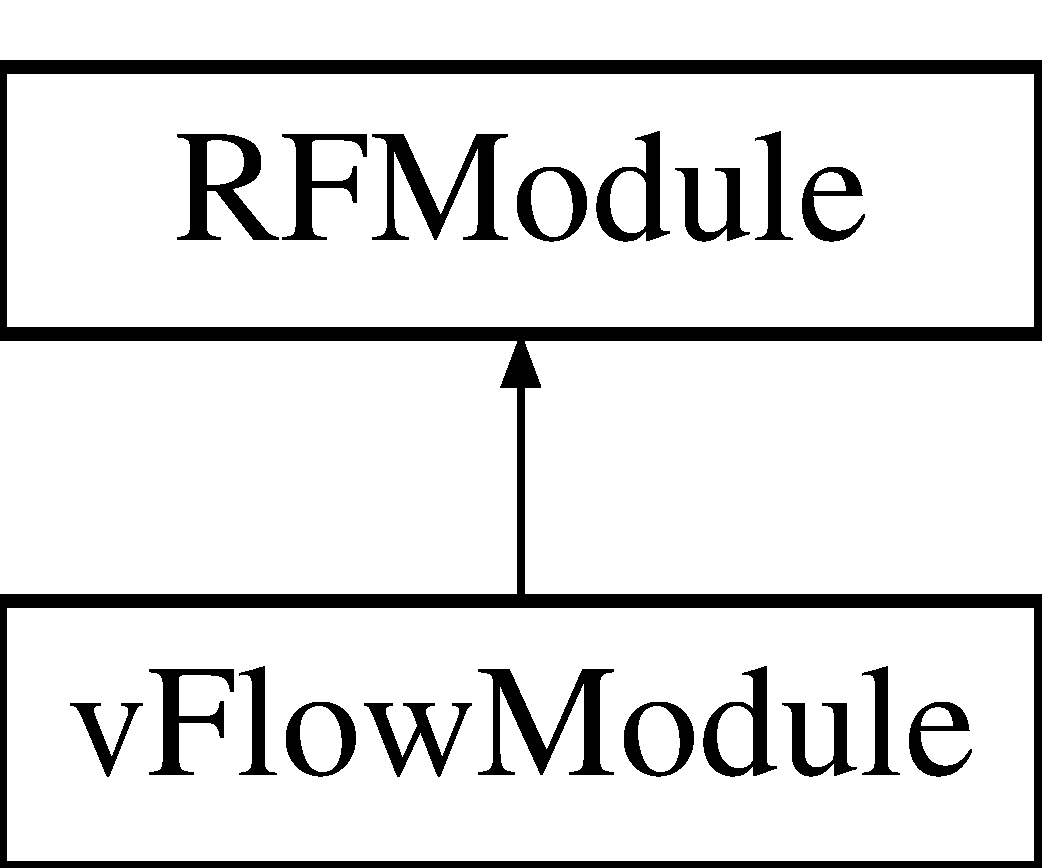
\includegraphics[height=2.000000cm]{classvFlowModule}
\end{center}
\end{figure}
\subsection*{Public Member Functions}
\begin{DoxyCompactItemize}
\item 
virtual bool {\bfseries configure} (yarp\+::os\+::\+Resource\+Finder \&rf)\hypertarget{classvFlowModule_a5cf91bc0de9e311b1946c6ec044fd947}{}\label{classvFlowModule_a5cf91bc0de9e311b1946c6ec044fd947}

\item 
virtual bool {\bfseries interrupt\+Module} ()\hypertarget{classvFlowModule_a49a90a2d595d99bf290423dd930eefe2}{}\label{classvFlowModule_a49a90a2d595d99bf290423dd930eefe2}

\item 
virtual bool {\bfseries close} ()\hypertarget{classvFlowModule_a63a3da2ac7ba9631753ea244d8bc4358}{}\label{classvFlowModule_a63a3da2ac7ba9631753ea244d8bc4358}

\item 
virtual bool {\bfseries update\+Module} ()\hypertarget{classvFlowModule_a880de21f5c85d684f7c0999d0a84e26b}{}\label{classvFlowModule_a880de21f5c85d684f7c0999d0a84e26b}

\item 
virtual double {\bfseries get\+Period} ()\hypertarget{classvFlowModule_a8f6f74c4a7888e162c2dff8a34a84323}{}\label{classvFlowModule_a8f6f74c4a7888e162c2dff8a34a84323}

\end{DoxyCompactItemize}


The documentation for this class was generated from the following files\+:\begin{DoxyCompactItemize}
\item 
/home/aglover/workspace/projects/event-\/driven/src/modules/v\+Flow/include/v\+Flow.\+h\item 
/home/aglover/workspace/projects/event-\/driven/src/modules/v\+Flow/src/v\+Flow.\+cpp\end{DoxyCompactItemize}

\hypertarget{classev_1_1vFuzzyEdge}{}\section{ev\+:\+:v\+Fuzzy\+Edge Class Reference}
\label{classev_1_1vFuzzyEdge}\index{ev\+::v\+Fuzzy\+Edge@{ev\+::v\+Fuzzy\+Edge}}
Inheritance diagram for ev\+:\+:v\+Fuzzy\+Edge\+:\begin{figure}[H]
\begin{center}
\leavevmode
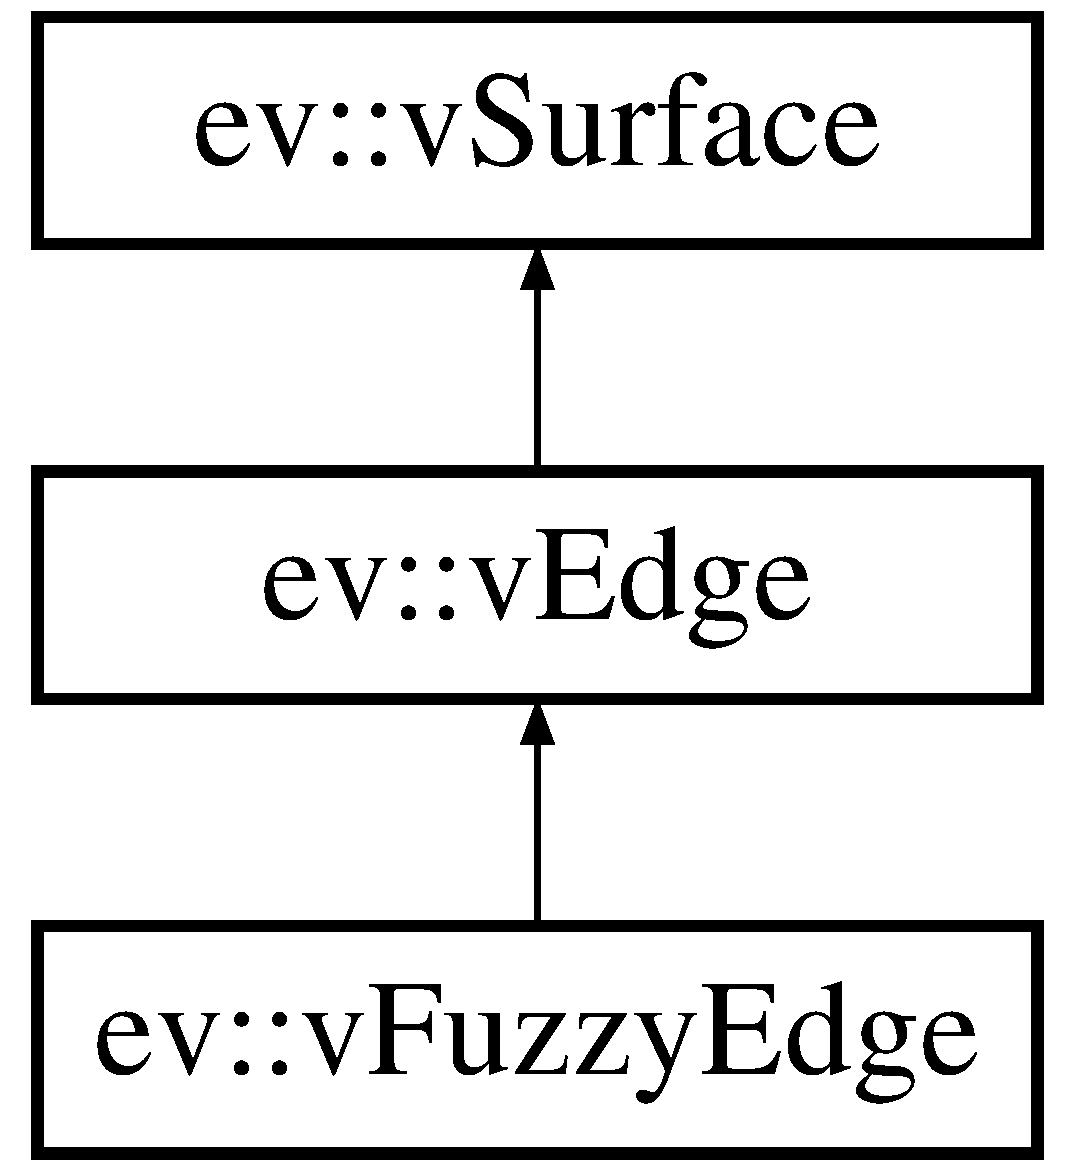
\includegraphics[height=3.000000cm]{classev_1_1vFuzzyEdge}
\end{center}
\end{figure}
\subsection*{Public Member Functions}
\begin{DoxyCompactItemize}
\item 
{\bfseries v\+Fuzzy\+Edge} (int \hyperlink{classev_1_1vSurface_a9666b7ae2580bf5647f65306f911825e}{width}=128, int \hyperlink{classev_1_1vSurface_ab3cf3df2f4fcb7eb5d89e0c5d1a5eeff}{height}=128, double delta=0.\+4)\hypertarget{classev_1_1vFuzzyEdge_a4fa6e20618a528a591baf2f098cace53}{}\label{classev_1_1vFuzzyEdge_a4fa6e20618a528a591baf2f098cace53}

\item 
\hyperlink{classev_1_1vQueue}{v\+Queue} {\bfseries add\+Event\+To\+Edge} (event$<$ \hyperlink{classev_1_1AddressEvent}{Address\+Event} $>$ event)\hypertarget{classev_1_1vFuzzyEdge_a61803b783119945df5c130c12d99e9c2}{}\label{classev_1_1vFuzzyEdge_a61803b783119945df5c130c12d99e9c2}

\item 
virtual const \hyperlink{classev_1_1vQueue}{v\+Queue} \& {\bfseries get\+S\+U\+RF} (int xl, int xh, int yl, int yh)\hypertarget{classev_1_1vFuzzyEdge_a8a495c6c2d878c7e047feebdd0a90b35}{}\label{classev_1_1vFuzzyEdge_a8a495c6c2d878c7e047feebdd0a90b35}

\end{DoxyCompactItemize}
\subsection*{Additional Inherited Members}


The documentation for this class was generated from the following files\+:\begin{DoxyCompactItemize}
\item 
/home/aglover/workspace/projects/event-\/driven/libraries/include/i\+Cub/eventdriven/v\+Surface.\+h\item 
/home/aglover/workspace/projects/event-\/driven/libraries/src/v\+Surface.\+cpp\end{DoxyCompactItemize}

\hypertarget{classvParticle}{}\section{v\+Particle Class Reference}
\label{classvParticle}\index{v\+Particle@{v\+Particle}}
\subsection*{Public Member Functions}
\begin{DoxyCompactItemize}
\item 
void {\bfseries setid} (int id)\hypertarget{classvParticle_a64262c584495ed46940724b4f645db42}{}\label{classvParticle_a64262c584495ed46940724b4f645db42}

\item 
int {\bfseries getid} ()\hypertarget{classvParticle_a121f7c012ccbb6153eda5bee38ba310b}{}\label{classvParticle_a121f7c012ccbb6153eda5bee38ba310b}

\item 
void {\bfseries init\+State} (double x, double y, double r, double vx, double vy, double vr)\hypertarget{classvParticle_a1f1f4121c044427f6a40658305a590c1}{}\label{classvParticle_a1f1f4121c044427f6a40658305a590c1}

\item 
void {\bfseries init\+State} (double x, double y, double r, double tw)\hypertarget{classvParticle_a7a3db503f06737b1752081fbd6fc3a1e}{}\label{classvParticle_a7a3db503f06737b1752081fbd6fc3a1e}

\item 
void {\bfseries init\+Timing} (unsigned long int stamp)\hypertarget{classvParticle_a32a3db438862056c87414bfd7ee61522}{}\label{classvParticle_a32a3db438862056c87414bfd7ee61522}

\item 
void {\bfseries init\+Weight} (double weight)\hypertarget{classvParticle_af4c313f241bb13b00d592f7dae686fd9}{}\label{classvParticle_af4c313f241bb13b00d592f7dae686fd9}

\item 
unsigned int {\bfseries get\+Temporal\+Window} ()\hypertarget{classvParticle_a4bc5705c6b9f4c518318f3d7c4cb7ed6}{}\label{classvParticle_a4bc5705c6b9f4c518318f3d7c4cb7ed6}

\item 
void {\bfseries set\+Rate} (unsigned int rate)\hypertarget{classvParticle_a9d9e636c612d03cd68cd1f1e06179249}{}\label{classvParticle_a9d9e636c612d03cd68cd1f1e06179249}

\item 
void {\bfseries resample} (double w, unsigned long int t)\hypertarget{classvParticle_a007403ab415b51a555ae5c8ef2d57ddd}{}\label{classvParticle_a007403ab415b51a555ae5c8ef2d57ddd}

\item 
void {\bfseries resample} (const \hyperlink{classvParticle}{v\+Particle} \&seeder, double w, unsigned long int t)\hypertarget{classvParticle_a62003dd534e9caa94ec9944148f2f319}{}\label{classvParticle_a62003dd534e9caa94ec9944148f2f319}

\item 
bool {\bfseries predict} (unsigned long int stamp)\hypertarget{classvParticle_a100f92e97462a7044766c6533b195380}{}\label{classvParticle_a100f92e97462a7044766c6533b195380}

\item 
double {\bfseries calc\+Likelihood} (\hyperlink{classev_1_1vQueue}{ev\+::v\+Queue} \&events, int nparticles)\hypertarget{classvParticle_ad1370073f2b84f2650f3c0ed147bc906}{}\label{classvParticle_ad1370073f2b84f2650f3c0ed147bc906}

\item 
void {\bfseries init\+Likelihood} ()\hypertarget{classvParticle_aeb6f48a94882492e7959cab8cc670714}{}\label{classvParticle_aeb6f48a94882492e7959cab8cc670714}

\item 
void {\bfseries incremental\+Likelihood} (int vx, int vy, int dt)\hypertarget{classvParticle_a48eb9de4510ca5ad9eb27fcad770af95}{}\label{classvParticle_a48eb9de4510ca5ad9eb27fcad770af95}

\item 
void {\bfseries conclude\+Likelihood} ()\hypertarget{classvParticle_ae16c098e00f11d2858edef59fc323c53}{}\label{classvParticle_ae16c098e00f11d2858edef59fc323c53}

\item 
void {\bfseries update\+Weight} (double l, double n)\hypertarget{classvParticle_acac9cb115f7ee7a1200e3ef8c389f948}{}\label{classvParticle_acac9cb115f7ee7a1200e3ef8c389f948}

\item 
void {\bfseries update\+Weight2} (double likelihood, double pwsumsq)\hypertarget{classvParticle_abf7b613d453af4e82e58a7eddc373f43}{}\label{classvParticle_abf7b613d453af4e82e58a7eddc373f43}

\item 
void {\bfseries update\+Weight\+Sync} (double normval)\hypertarget{classvParticle_a71ac3f26d797818df2c671cb63ef5a60}{}\label{classvParticle_a71ac3f26d797818df2c671cb63ef5a60}

\item 
double {\bfseries getx} ()\hypertarget{classvParticle_a3d198bc0a1b1a475ab0b044bbff61488}{}\label{classvParticle_a3d198bc0a1b1a475ab0b044bbff61488}

\item 
double {\bfseries gety} ()\hypertarget{classvParticle_a40050ef035199b05e7cfd2601003d68a}{}\label{classvParticle_a40050ef035199b05e7cfd2601003d68a}

\item 
double {\bfseries getr} ()\hypertarget{classvParticle_ac78d2469a78798f791a5dab9f69b732e}{}\label{classvParticle_ac78d2469a78798f791a5dab9f69b732e}

\item 
double {\bfseries getw} ()\hypertarget{classvParticle_ac75939f4ac46ee086991fb629c583ada}{}\label{classvParticle_ac75939f4ac46ee086991fb629c583ada}

\item 
double {\bfseries getl} ()\hypertarget{classvParticle_a9b43157a0b2b278873c78806ccd75f6f}{}\label{classvParticle_a9b43157a0b2b278873c78806ccd75f6f}

\item 
double {\bfseries gettw} ()\hypertarget{classvParticle_a1760cb3cbd3014e6f5cf0a55e5d4dfff}{}\label{classvParticle_a1760cb3cbd3014e6f5cf0a55e5d4dfff}

\item 
unsigned long {\bfseries get\+Update\+Time} ()\hypertarget{classvParticle_aa866c2138932659daa4b4bf5fb066127}{}\label{classvParticle_aa866c2138932659daa4b4bf5fb066127}

\item 
unsigned long {\bfseries get\+Stamp} ()\hypertarget{classvParticle_af3b6763f2a1934d6f0cd470d3f1ea830}{}\label{classvParticle_af3b6763f2a1934d6f0cd470d3f1ea830}

\item 
bool {\bfseries needs\+Updating} (unsigned long int stamp)\hypertarget{classvParticle_a40088530921a6cdcc80f6ec56f6ff50f}{}\label{classvParticle_a40088530921a6cdcc80f6ec56f6ff50f}

\item 
bool {\bfseries operator$<$} (const \hyperlink{classvParticle}{v\+Particle} \&p) const \hypertarget{classvParticle_a5f1d15db973dbc077ed6f1b30a6fc9bf}{}\label{classvParticle_a5f1d15db973dbc077ed6f1b30a6fc9bf}

\item 
bool {\bfseries operator$>$} (const \hyperlink{classvParticle}{v\+Particle} \&p) const \hypertarget{classvParticle_ab62ea7572f30877c05f917c4f7c04416}{}\label{classvParticle_ab62ea7572f30877c05f917c4f7c04416}

\end{DoxyCompactItemize}


The documentation for this class was generated from the following files\+:\begin{DoxyCompactItemize}
\item 
/home/aglover/workspace/projects/event-\/driven/src/modules/v\+Particle\+Filter/include/v\+Particle\+Filter.\+h\item 
/home/aglover/workspace/projects/event-\/driven/src/modules/v\+Particle\+Filter/src/v\+Particle\+Filter.\+cpp\end{DoxyCompactItemize}

\hypertarget{classvParticleModule}{}\section{v\+Particle\+Module Class Reference}
\label{classvParticleModule}\index{v\+Particle\+Module@{v\+Particle\+Module}}
Inheritance diagram for v\+Particle\+Module\+:\begin{figure}[H]
\begin{center}
\leavevmode
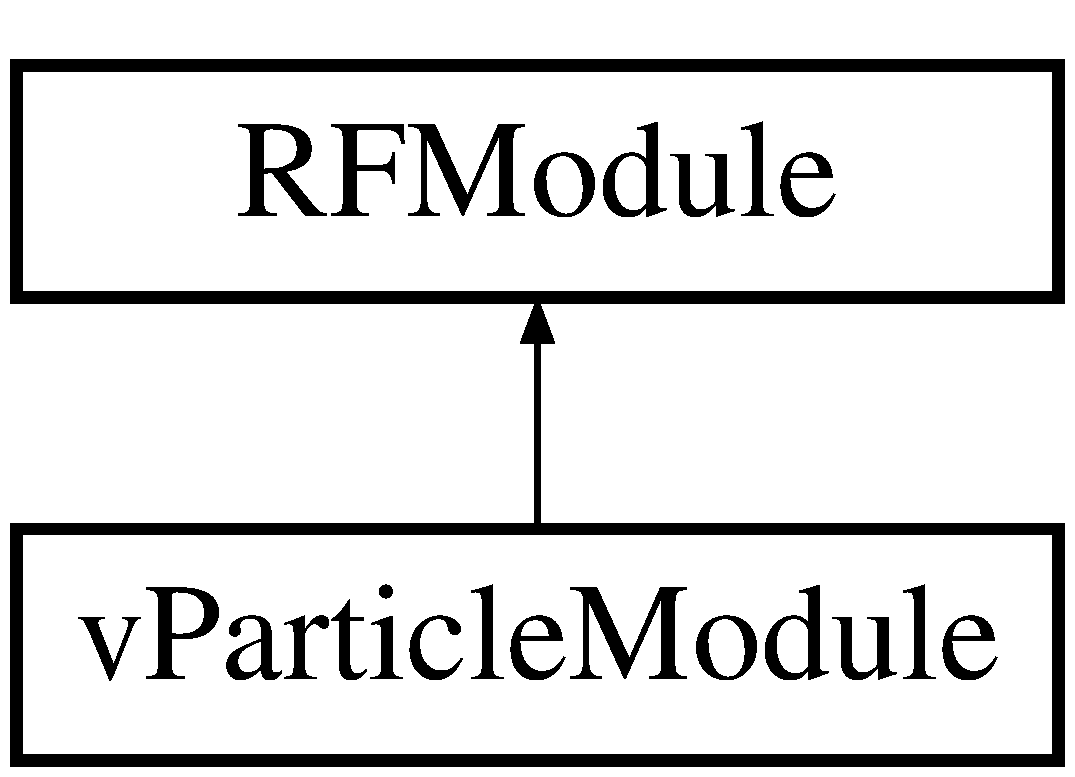
\includegraphics[height=2.000000cm]{classvParticleModule}
\end{center}
\end{figure}
\subsection*{Public Member Functions}
\begin{DoxyCompactItemize}
\item 
virtual bool {\bfseries configure} (yarp\+::os\+::\+Resource\+Finder \&rf)\hypertarget{classvParticleModule_a50220d0e8c348cbb887924def82ec78b}{}\label{classvParticleModule_a50220d0e8c348cbb887924def82ec78b}

\item 
virtual bool {\bfseries interrupt\+Module} ()\hypertarget{classvParticleModule_ae0dbee0680f7006c09a2413d13cbb4fb}{}\label{classvParticleModule_ae0dbee0680f7006c09a2413d13cbb4fb}

\item 
virtual bool {\bfseries close} ()\hypertarget{classvParticleModule_a622f526fc7e2e194b301ff1fa6a362bb}{}\label{classvParticleModule_a622f526fc7e2e194b301ff1fa6a362bb}

\item 
virtual double {\bfseries get\+Period} ()\hypertarget{classvParticleModule_acee72c3ad5f6eddb580fbf57f0cb9d7e}{}\label{classvParticleModule_acee72c3ad5f6eddb580fbf57f0cb9d7e}

\item 
virtual bool {\bfseries update\+Module} ()\hypertarget{classvParticleModule_ae1973b925b09372518b4922b8f033363}{}\label{classvParticleModule_ae1973b925b09372518b4922b8f033363}

\end{DoxyCompactItemize}


The documentation for this class was generated from the following files\+:\begin{DoxyCompactItemize}
\item 
/home/aglover/workspace/projects/event-\/driven/src/modules/v\+Particle\+Filter/include/v\+Particle\+Module.\+h\item 
/home/aglover/workspace/projects/event-\/driven/src/modules/v\+Particle\+Filter/src/v\+Particle\+Module.\+cpp\end{DoxyCompactItemize}

\hypertarget{classvParticleReader}{}\section{v\+Particle\+Reader Class Reference}
\label{classvParticleReader}\index{v\+Particle\+Reader@{v\+Particle\+Reader}}
Inheritance diagram for v\+Particle\+Reader\+:\begin{figure}[H]
\begin{center}
\leavevmode
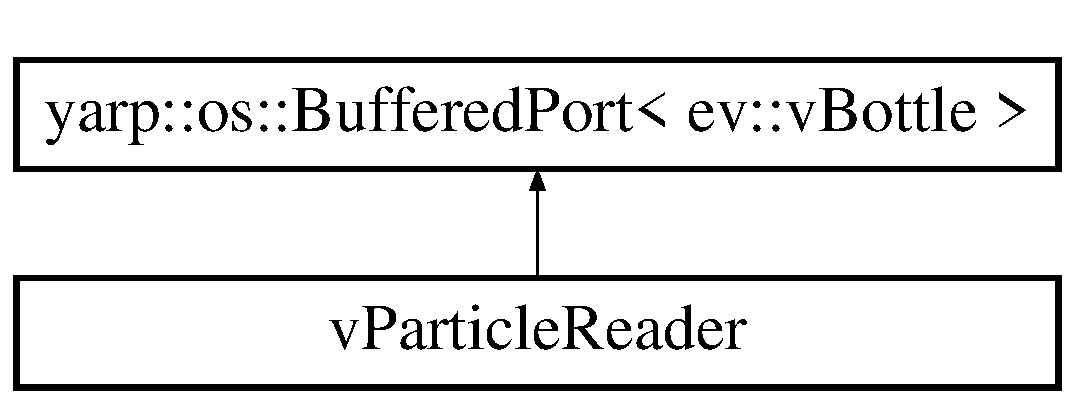
\includegraphics[height=2.000000cm]{classvParticleReader}
\end{center}
\end{figure}
\subsection*{Public Member Functions}
\begin{DoxyCompactItemize}
\item 
{\bfseries v\+Particle\+Reader} (unsigned int width=128, unsigned int height=128)\hypertarget{classvParticleReader_aa845b76dd7066a16984dd3277a8f2e6d}{}\label{classvParticleReader_aa845b76dd7066a16984dd3277a8f2e6d}

\item 
bool {\bfseries open} (const std\+::string \&name, bool strictness=false)\hypertarget{classvParticleReader_a758adac809850f3fc1f01d2502d609bc}{}\label{classvParticleReader_a758adac809850f3fc1f01d2502d609bc}

\item 
void {\bfseries on\+Read} (\hyperlink{classev_1_1vBottle}{ev\+::v\+Bottle} \&in\+Bot)\hypertarget{classvParticleReader_af4bb9d631985a90d797416eca04777bb}{}\label{classvParticleReader_af4bb9d631985a90d797416eca04777bb}

\item 
void {\bfseries close} ()\hypertarget{classvParticleReader_a727d94974d16c502ac2518c5760e0fcc}{}\label{classvParticleReader_a727d94974d16c502ac2518c5760e0fcc}

\item 
void {\bfseries interrupt} ()\hypertarget{classvParticleReader_af7e95400429bb07bc9a438f8a163023e}{}\label{classvParticleReader_af7e95400429bb07bc9a438f8a163023e}

\end{DoxyCompactItemize}


The documentation for this class was generated from the following files\+:\begin{DoxyCompactItemize}
\item 
/home/aglover/workspace/projects/event-\/driven/src/modules/v\+Particle\+Filter/include/v\+Particle\+Module.\+h\item 
/home/aglover/workspace/projects/event-\/driven/src/modules/v\+Particle\+Filter/src/v\+Particle\+Module.\+cpp\end{DoxyCompactItemize}

\hypertarget{classvPartObsThread}{}\section{v\+Part\+Obs\+Thread Class Reference}
\label{classvPartObsThread}\index{v\+Part\+Obs\+Thread@{v\+Part\+Obs\+Thread}}
Inheritance diagram for v\+Part\+Obs\+Thread\+:\begin{figure}[H]
\begin{center}
\leavevmode
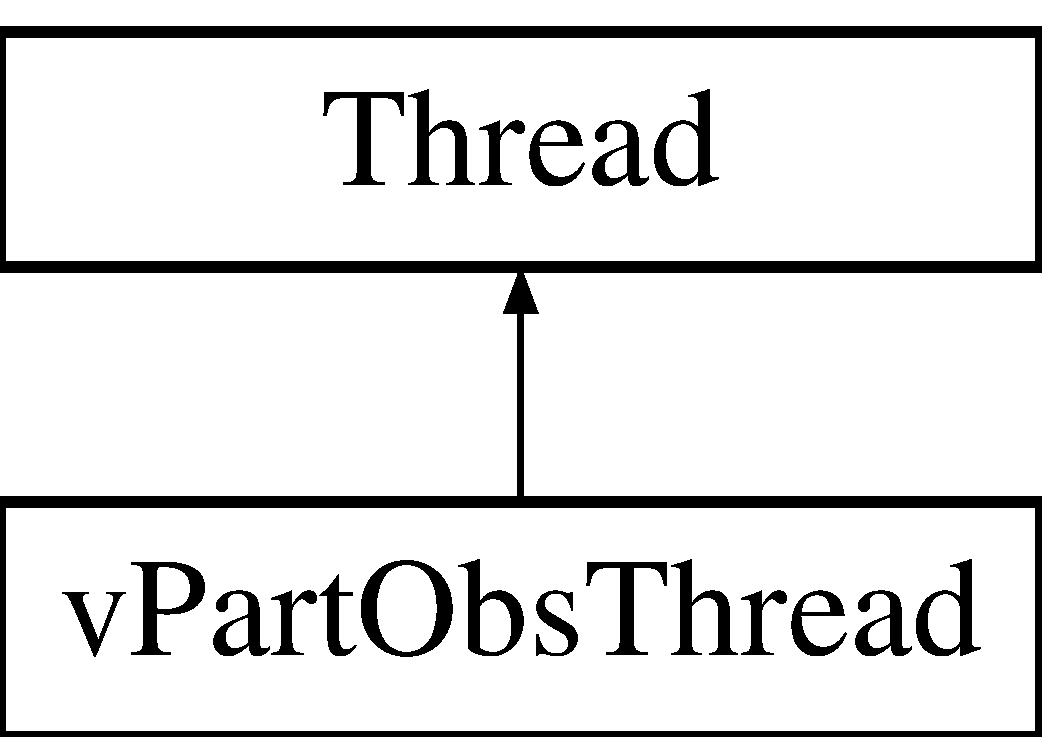
\includegraphics[height=2.000000cm]{classvPartObsThread}
\end{center}
\end{figure}
\subsection*{Public Member Functions}
\begin{DoxyCompactItemize}
\item 
{\bfseries v\+Part\+Obs\+Thread} (int p\+Start, int p\+End)\hypertarget{classvPartObsThread_ad5ee91bcd5ace1cac76ac13843597d3d}{}\label{classvPartObsThread_ad5ee91bcd5ace1cac76ac13843597d3d}

\item 
void {\bfseries set\+Data\+Sources} (std\+::vector$<$ \hyperlink{classvParticle}{v\+Particle} $>$ $\ast$particles, std\+::vector$<$ int $>$ $\ast$deltats, \hyperlink{classev_1_1vQueue}{ev\+::v\+Queue} $\ast$stw)\hypertarget{classvPartObsThread_aedc0c0ef46d5cc48754621b41936a23d}{}\label{classvPartObsThread_aedc0c0ef46d5cc48754621b41936a23d}

\item 
double {\bfseries get\+Norm\+Val} ()\hypertarget{classvPartObsThread_a2bc5cbff69dd31bd7b571579d6b34930}{}\label{classvPartObsThread_a2bc5cbff69dd31bd7b571579d6b34930}

\item 
bool {\bfseries thread\+Init} ()\hypertarget{classvPartObsThread_a5814f390e326d1bd4cfa82e34855d3d4}{}\label{classvPartObsThread_a5814f390e326d1bd4cfa82e34855d3d4}

\item 
void {\bfseries run} ()\hypertarget{classvPartObsThread_ae261ba48ff6af1ad105adc5ed8fd5373}{}\label{classvPartObsThread_ae261ba48ff6af1ad105adc5ed8fd5373}

\item 
void {\bfseries thread\+Release} ()\hypertarget{classvPartObsThread_a080024e2fc09ae2e3ca16b686d9a2791}{}\label{classvPartObsThread_a080024e2fc09ae2e3ca16b686d9a2791}

\end{DoxyCompactItemize}


The documentation for this class was generated from the following files\+:\begin{DoxyCompactItemize}
\item 
/home/aglover/workspace/projects/event-\/driven/src/modules/v\+Particle\+Filter/include/v\+Particle\+Module.\+h\item 
/home/aglover/workspace/projects/event-\/driven/src/modules/v\+Particle\+Filter/src/v\+Particle\+Module.\+cpp\end{DoxyCompactItemize}

\hypertarget{classev_1_1vQueue}{}\section{ev\+:\+:v\+Queue Class Reference}
\label{classev_1_1vQueue}\index{ev\+::v\+Queue@{ev\+::v\+Queue}}
Inheritance diagram for ev\+:\+:v\+Queue\+:\begin{figure}[H]
\begin{center}
\leavevmode
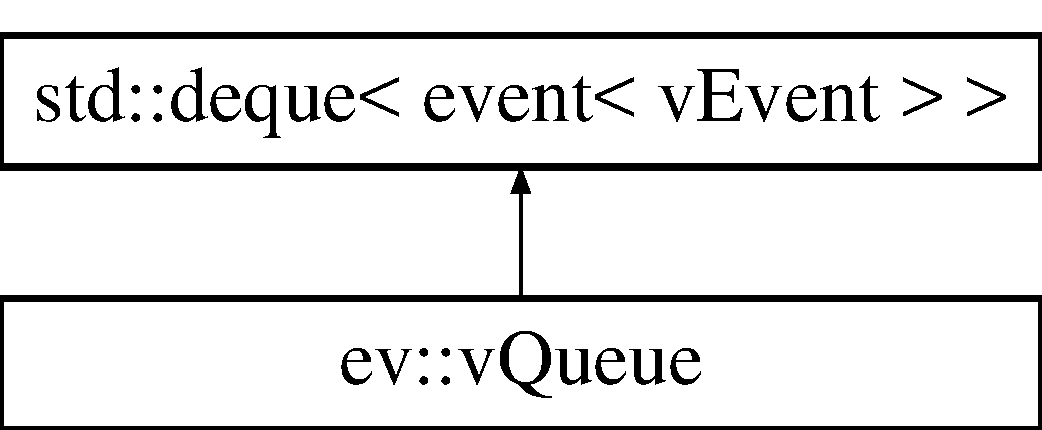
\includegraphics[height=2.000000cm]{classev_1_1vQueue}
\end{center}
\end{figure}
\subsection*{Public Member Functions}
\begin{DoxyCompactItemize}
\item 
void {\bfseries sort} (bool respect\+Wraps=false)\hypertarget{classev_1_1vQueue_a40d7fe7c3ddca1eb9c567c0f50fede79}{}\label{classev_1_1vQueue_a40d7fe7c3ddca1eb9c567c0f50fede79}

\end{DoxyCompactItemize}


The documentation for this class was generated from the following files\+:\begin{DoxyCompactItemize}
\item 
/home/aglover/workspace/projects/event-\/driven/libraries/include/i\+Cub/eventdriven/v\+Queue.\+h\item 
/home/aglover/workspace/projects/event-\/driven/libraries/src/v\+Queue.\+cpp\end{DoxyCompactItemize}

\hypertarget{classvRepTest}{}\section{v\+Rep\+Test Class Reference}
\label{classvRepTest}\index{v\+Rep\+Test@{v\+Rep\+Test}}
Inheritance diagram for v\+Rep\+Test\+:\begin{figure}[H]
\begin{center}
\leavevmode
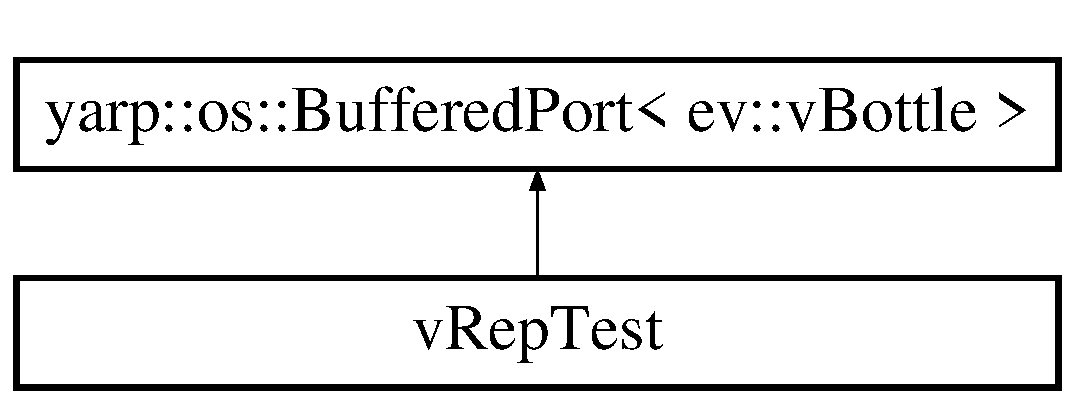
\includegraphics[height=2.000000cm]{classvRepTest}
\end{center}
\end{figure}
\subsection*{Public Member Functions}
\begin{DoxyCompactItemize}
\item 
void {\bfseries set\+Temporal\+Window} (int dt)\hypertarget{classvRepTest_afc9888397eba6894a65302b0226d81f0}{}\label{classvRepTest_afc9888397eba6894a65302b0226d81f0}

\item 
void {\bfseries set\+Fixed\+Window} (int N)\hypertarget{classvRepTest_a72524b413a72d7a56f48e1a4f2021177}{}\label{classvRepTest_a72524b413a72d7a56f48e1a4f2021177}

\item 
void {\bfseries set\+Vis\+Type} (std\+::string vis)\hypertarget{classvRepTest_aa616d24c44c0f452a42f4b02e4395967}{}\label{classvRepTest_aa616d24c44c0f452a42f4b02e4395967}

\item 
bool {\bfseries open} (const std\+::string \&name, bool strict=false)\hypertarget{classvRepTest_a02ae7ad9d91210b42178b45e3b0a7d68}{}\label{classvRepTest_a02ae7ad9d91210b42178b45e3b0a7d68}

\item 
void {\bfseries close} ()\hypertarget{classvRepTest_a95d46a88b378bb620c4ee3c0e1c7f32a}{}\label{classvRepTest_a95d46a88b378bb620c4ee3c0e1c7f32a}

\item 
void {\bfseries interrupt} ()\hypertarget{classvRepTest_aed45d04a505f13efba3cfc64bc59d795}{}\label{classvRepTest_aed45d04a505f13efba3cfc64bc59d795}

\item 
void {\bfseries on\+Read} (\hyperlink{classev_1_1vBottle}{ev\+::v\+Bottle} \&in\+Bottle)\hypertarget{classvRepTest_aea8bca9d38eed370dd7969063d93d229}{}\label{classvRepTest_aea8bca9d38eed370dd7969063d93d229}

\end{DoxyCompactItemize}


The documentation for this class was generated from the following files\+:\begin{DoxyCompactItemize}
\item 
/home/aglover/workspace/projects/event-\/driven/src/modules/v\+Rep\+Test/include/v\+Rep\+Test.\+h\item 
/home/aglover/workspace/projects/event-\/driven/src/modules/v\+Rep\+Test/src/v\+Rep\+Test.\+cpp\end{DoxyCompactItemize}

\hypertarget{classvRepTestHandler}{}\section{v\+Rep\+Test\+Handler Class Reference}
\label{classvRepTestHandler}\index{v\+Rep\+Test\+Handler@{v\+Rep\+Test\+Handler}}
Inheritance diagram for v\+Rep\+Test\+Handler\+:\begin{figure}[H]
\begin{center}
\leavevmode
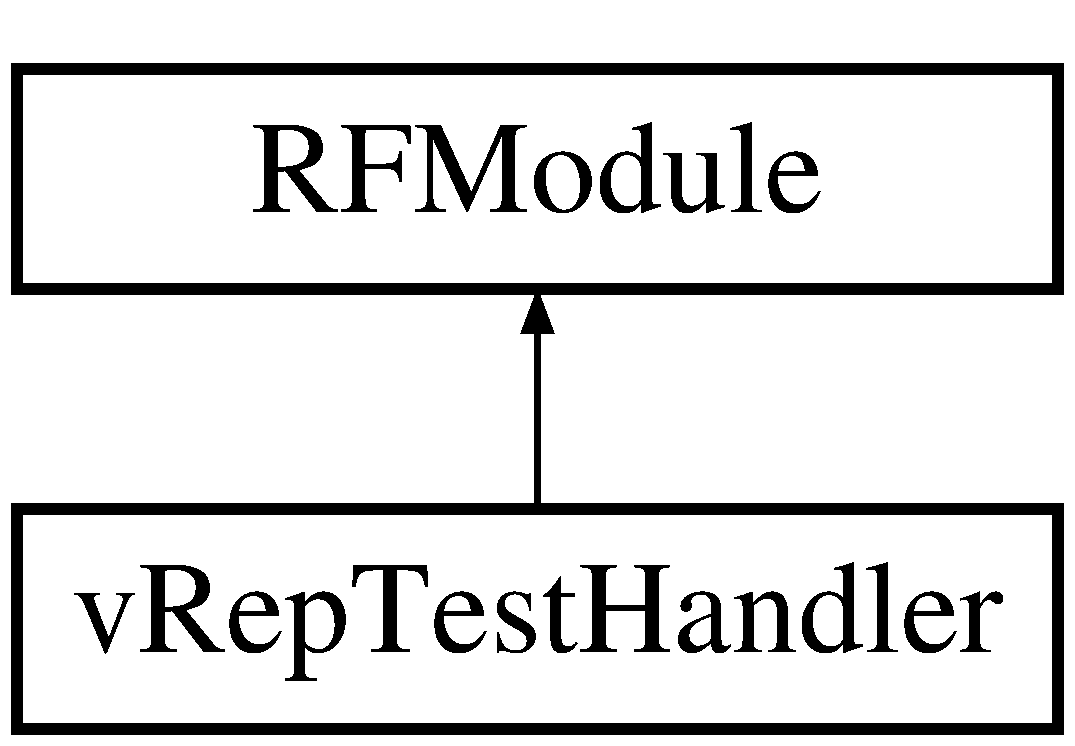
\includegraphics[height=2.000000cm]{classvRepTestHandler}
\end{center}
\end{figure}
\subsection*{Public Member Functions}
\begin{DoxyCompactItemize}
\item 
virtual bool {\bfseries configure} (yarp\+::os\+::\+Resource\+Finder \&rf)\hypertarget{classvRepTestHandler_a75d6ab4e2998eccf96b0f90b53d183f3}{}\label{classvRepTestHandler_a75d6ab4e2998eccf96b0f90b53d183f3}

\item 
virtual bool {\bfseries interrupt\+Module} ()\hypertarget{classvRepTestHandler_aa67c736991dc0601e5775b8f60b680be}{}\label{classvRepTestHandler_aa67c736991dc0601e5775b8f60b680be}

\item 
virtual bool {\bfseries close} ()\hypertarget{classvRepTestHandler_ad40900db7b64a3b8539834ff18ddc2c1}{}\label{classvRepTestHandler_ad40900db7b64a3b8539834ff18ddc2c1}

\item 
virtual double {\bfseries get\+Period} ()\hypertarget{classvRepTestHandler_a53456bbfb2edf31921b6b775b3bc1119}{}\label{classvRepTestHandler_a53456bbfb2edf31921b6b775b3bc1119}

\item 
virtual bool {\bfseries update\+Module} ()\hypertarget{classvRepTestHandler_a307f808f4e474d8b7c352e346cbda80b}{}\label{classvRepTestHandler_a307f808f4e474d8b7c352e346cbda80b}

\end{DoxyCompactItemize}


The documentation for this class was generated from the following files\+:\begin{DoxyCompactItemize}
\item 
/home/aglover/workspace/projects/event-\/driven/src/modules/v\+Rep\+Test/include/v\+Rep\+Test.\+h\item 
/home/aglover/workspace/projects/event-\/driven/src/modules/v\+Rep\+Test/src/v\+Rep\+Test.\+cpp\end{DoxyCompactItemize}

\hypertarget{classvSalientPos}{}\section{v\+Salient\+Pos Class Reference}
\label{classvSalientPos}\index{v\+Salient\+Pos@{v\+Salient\+Pos}}
Inheritance diagram for v\+Salient\+Pos\+:\begin{figure}[H]
\begin{center}
\leavevmode
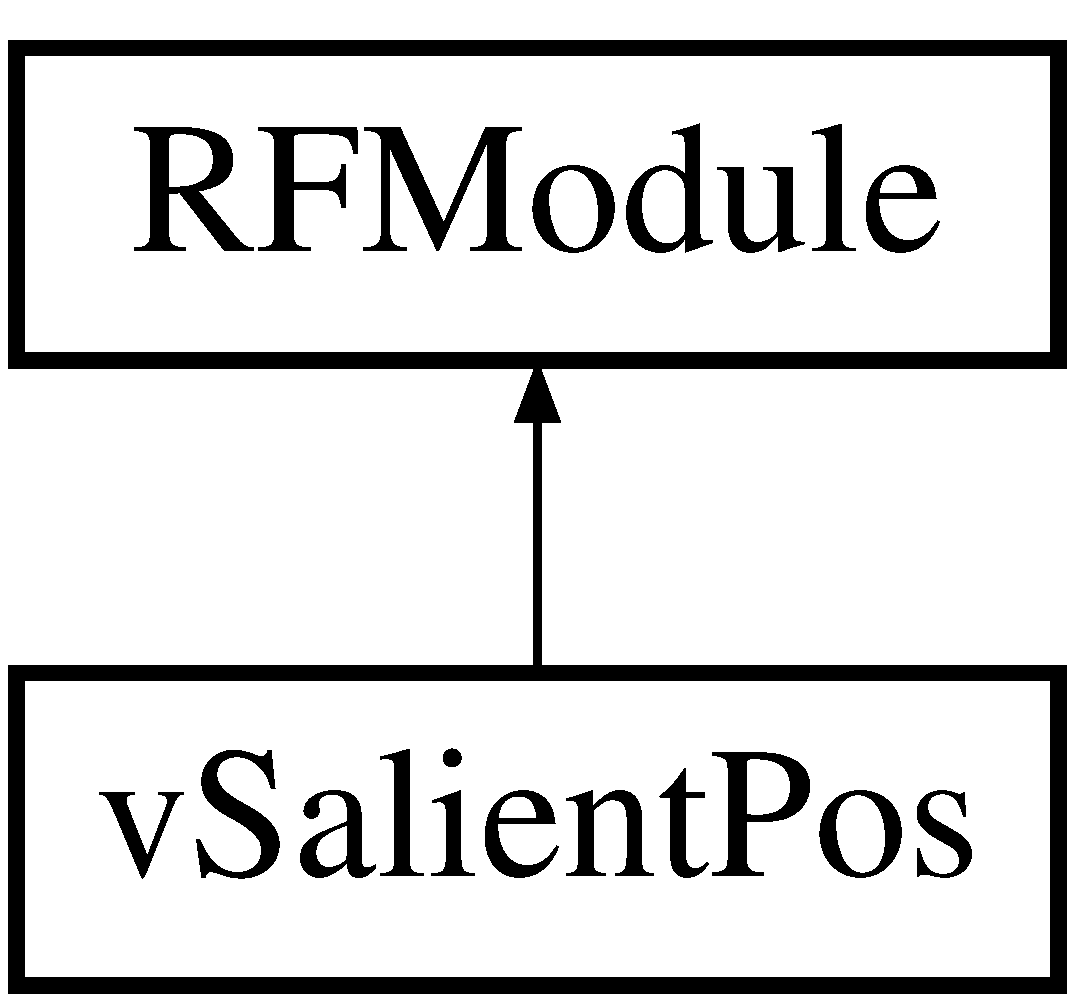
\includegraphics[height=2.000000cm]{classvSalientPos}
\end{center}
\end{figure}
\subsection*{Public Member Functions}
\begin{DoxyCompactItemize}
\item 
virtual bool {\bfseries configure} (yarp\+::os\+::\+Resource\+Finder \&rf)\hypertarget{classvSalientPos_ad46801e5962743b241c9f243e320c329}{}\label{classvSalientPos_ad46801e5962743b241c9f243e320c329}

\item 
virtual bool {\bfseries interrupt\+Module} ()\hypertarget{classvSalientPos_a08cf9e09b085f3886a849ee1d2b077b2}{}\label{classvSalientPos_a08cf9e09b085f3886a849ee1d2b077b2}

\item 
virtual bool {\bfseries close} ()\hypertarget{classvSalientPos_a95f359c8ad4525369cf38b907d79be11}{}\label{classvSalientPos_a95f359c8ad4525369cf38b907d79be11}

\item 
virtual double {\bfseries get\+Period} ()\hypertarget{classvSalientPos_adec841e273c2657901cdac84c7c60013}{}\label{classvSalientPos_adec841e273c2657901cdac84c7c60013}

\item 
virtual bool {\bfseries update\+Module} ()\hypertarget{classvSalientPos_a510d6422462efc0aa7cd413c35046e41}{}\label{classvSalientPos_a510d6422462efc0aa7cd413c35046e41}

\end{DoxyCompactItemize}


The documentation for this class was generated from the following files\+:\begin{DoxyCompactItemize}
\item 
/home/aglover/workspace/projects/event-\/driven/src/modules/salient\+Pos/include/salient\+Pos.\+h\item 
/home/aglover/workspace/projects/event-\/driven/src/modules/salient\+Pos/src/salient\+Pos.\+cpp\end{DoxyCompactItemize}

\hypertarget{classvSpinInterface}{}\section{v\+Spin\+Interface Class Reference}
\label{classvSpinInterface}\index{v\+Spin\+Interface@{v\+Spin\+Interface}}
Inheritance diagram for v\+Spin\+Interface\+:\begin{figure}[H]
\begin{center}
\leavevmode
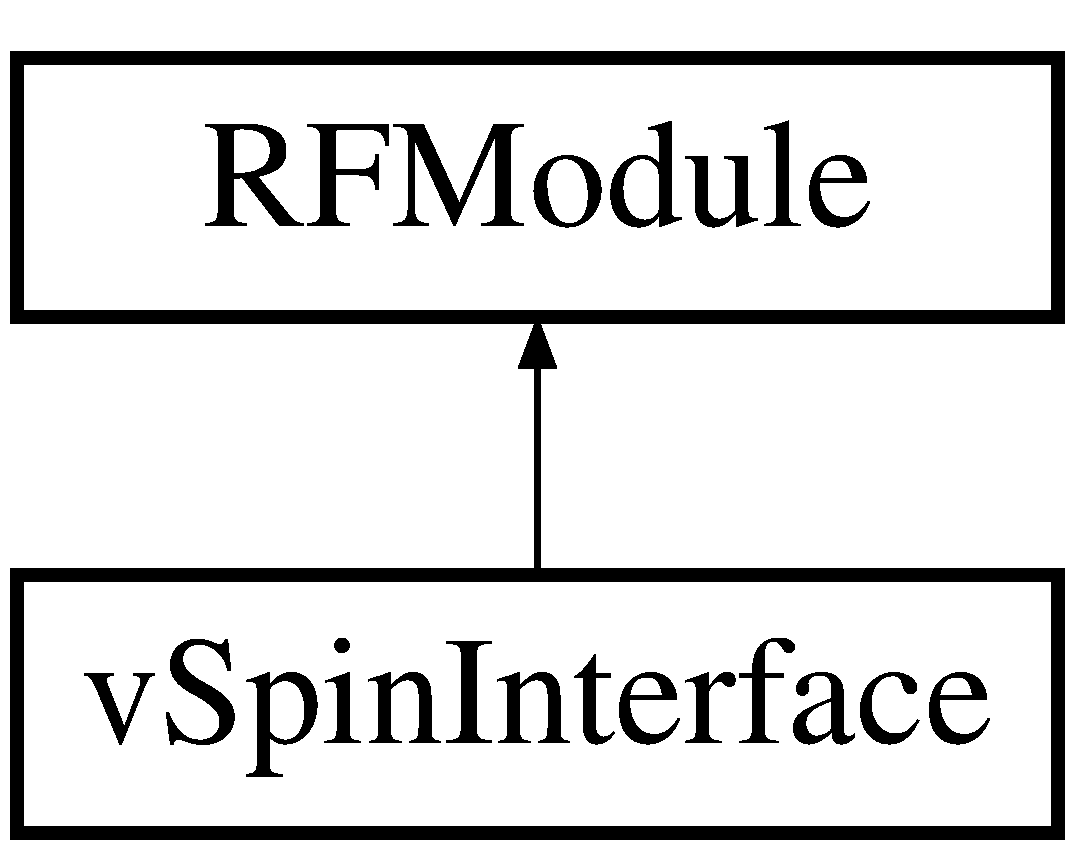
\includegraphics[height=2.000000cm]{classvSpinInterface}
\end{center}
\end{figure}
\subsection*{Public Member Functions}
\begin{DoxyCompactItemize}
\item 
virtual bool {\bfseries configure} (yarp\+::os\+::\+Resource\+Finder \&rf)\hypertarget{classvSpinInterface_afa8c4507f693729d5bf386e1190f5fbd}{}\label{classvSpinInterface_afa8c4507f693729d5bf386e1190f5fbd}

\item 
virtual bool {\bfseries interrupt\+Module} ()\hypertarget{classvSpinInterface_aa753c1ae6164708bea1fc3f01cd7f7b9}{}\label{classvSpinInterface_aa753c1ae6164708bea1fc3f01cd7f7b9}

\item 
virtual bool {\bfseries close} ()\hypertarget{classvSpinInterface_a832b19fa38602881e73cb5cea22ccb10}{}\label{classvSpinInterface_a832b19fa38602881e73cb5cea22ccb10}

\item 
virtual double {\bfseries get\+Period} ()\hypertarget{classvSpinInterface_a1addee84aa2d49ce627dd75b10a41f56}{}\label{classvSpinInterface_a1addee84aa2d49ce627dd75b10a41f56}

\item 
virtual bool {\bfseries update\+Module} ()\hypertarget{classvSpinInterface_a851d85f358a3225b18700cc2657eddff}{}\label{classvSpinInterface_a851d85f358a3225b18700cc2657eddff}

\end{DoxyCompactItemize}


The documentation for this class was generated from the following files\+:\begin{DoxyCompactItemize}
\item 
/home/aglover/workspace/projects/event-\/driven/src/hardwareio/spinterface/include/spinterface.\+h\item 
/home/aglover/workspace/projects/event-\/driven/src/hardwareio/spinterface/src/spinterface.\+cpp\end{DoxyCompactItemize}

\hypertarget{classev_1_1vSurface}{}\section{ev\+:\+:v\+Surface Class Reference}
\label{classev_1_1vSurface}\index{ev\+::v\+Surface@{ev\+::v\+Surface}}


The v\+Window class holds a list of events for a period of time as specified. Event expiry is checked each time new events are added and expired events are removed. At any point in time a copy of the current list of events can be requested.  




{\ttfamily \#include $<$v\+Surface.\+h$>$}

Inheritance diagram for ev\+:\+:v\+Surface\+:\begin{figure}[H]
\begin{center}
\leavevmode
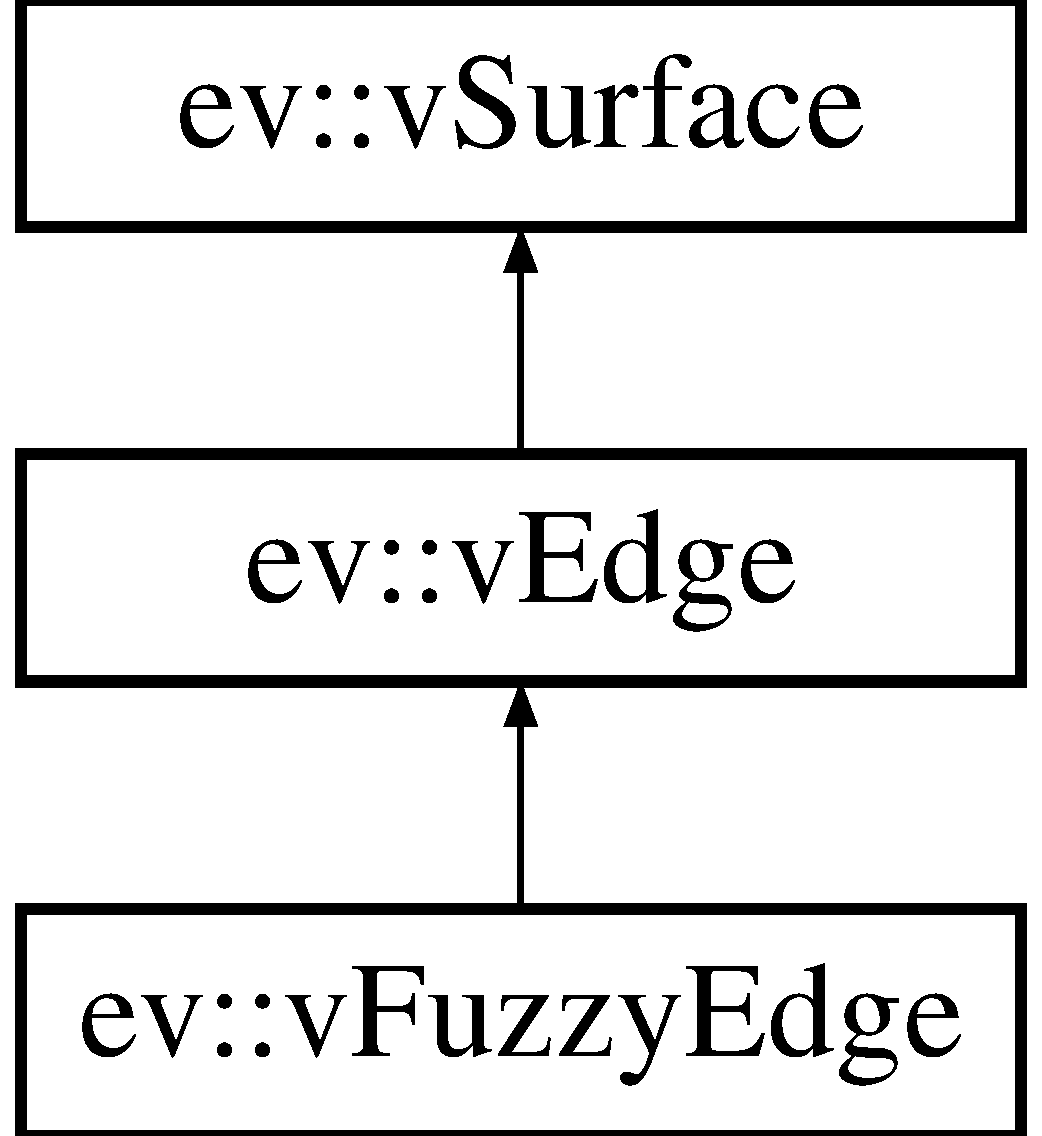
\includegraphics[height=3.000000cm]{classev_1_1vSurface}
\end{center}
\end{figure}
\subsection*{Public Member Functions}
\begin{DoxyCompactItemize}
\item 
\hyperlink{classev_1_1vSurface_afb642ce656aee165c54a2238474599c0}{v\+Surface} (int \hyperlink{classev_1_1vSurface_a9666b7ae2580bf5647f65306f911825e}{width}=128, int \hyperlink{classev_1_1vSurface_ab3cf3df2f4fcb7eb5d89e0c5d1a5eeff}{height}=128)
\begin{DoxyCompactList}\small\item\em v\+Window constructor \end{DoxyCompactList}\item 
{\bfseries v\+Surface} (const \hyperlink{classev_1_1vSurface}{v\+Surface} \&)\hypertarget{classev_1_1vSurface_a592c1c79ff294f34e28503d7c7278b8f}{}\label{classev_1_1vSurface_a592c1c79ff294f34e28503d7c7278b8f}

\item 
\hyperlink{classev_1_1vSurface}{v\+Surface} {\bfseries operator=} (const \hyperlink{classev_1_1vSurface}{v\+Surface} \&)\hypertarget{classev_1_1vSurface_af779bb51b4c9f748a0cd38117cf5e1f9}{}\label{classev_1_1vSurface_af779bb51b4c9f748a0cd38117cf5e1f9}

\item 
event \hyperlink{classev_1_1vSurface_abb5a735613b4165a49a0da37f0770055}{add\+Event} (event$<$ \hyperlink{classev_1_1AddressEvent}{Address\+Event} $>$ v)
\begin{DoxyCompactList}\small\item\em add\+Event adds an event to the window. Also checks for expired events. \end{DoxyCompactList}\item 
event \hyperlink{classev_1_1vSurface_a4772b37a82726d86313438f5d89b2f62}{get\+Most\+Recent} ()
\begin{DoxyCompactList}\small\item\em get\+Most\+Recent \end{DoxyCompactList}\item 
int {\bfseries get\+Event\+Count} ()\hypertarget{classev_1_1vSurface_aa90e7d977149ee42dff7a2735b367a2b}{}\label{classev_1_1vSurface_aa90e7d977149ee42dff7a2735b367a2b}

\item 
void {\bfseries clear} ()\hypertarget{classev_1_1vSurface_a222eadfa9d900d22148d1ffb0bb68661}{}\label{classev_1_1vSurface_a222eadfa9d900d22148d1ffb0bb68661}

\item 
const \hyperlink{classev_1_1vQueue}{v\+Queue} \& {\bfseries get\+Surf} (int d)\hypertarget{classev_1_1vSurface_a16704556a7d824ab59b6250caa4d3c0b}{}\label{classev_1_1vSurface_a16704556a7d824ab59b6250caa4d3c0b}

\item 
const \hyperlink{classev_1_1vQueue}{v\+Queue} \& {\bfseries get\+Surf} (int x, int y, int d)\hypertarget{classev_1_1vSurface_aef72b92ba02f7e6a3e804a995cdf7894}{}\label{classev_1_1vSurface_aef72b92ba02f7e6a3e804a995cdf7894}

\item 
virtual const \hyperlink{classev_1_1vQueue}{v\+Queue} \& {\bfseries get\+Surf} (int xl, int xh, int yl, int yh)\hypertarget{classev_1_1vSurface_ad0364e9a0811fbbe46784c993b5fef31}{}\label{classev_1_1vSurface_ad0364e9a0811fbbe46784c993b5fef31}

\end{DoxyCompactItemize}
\subsection*{Protected Attributes}
\begin{DoxyCompactItemize}
\item 
std\+::vector$<$ std\+::vector$<$ event$<$$>$ $>$ $>$ \hyperlink{classev_1_1vSurface_ae75428cabd7e9eabc544d4ef7290e9e7}{spatial}\hypertarget{classev_1_1vSurface_ae75428cabd7e9eabc544d4ef7290e9e7}{}\label{classev_1_1vSurface_ae75428cabd7e9eabc544d4ef7290e9e7}

\begin{DoxyCompactList}\small\item\em for quick spatial accessing and surfacing \end{DoxyCompactList}\item 
int \hyperlink{classev_1_1vSurface_a9666b7ae2580bf5647f65306f911825e}{width}\hypertarget{classev_1_1vSurface_a9666b7ae2580bf5647f65306f911825e}{}\label{classev_1_1vSurface_a9666b7ae2580bf5647f65306f911825e}

\begin{DoxyCompactList}\small\item\em the sensor width \end{DoxyCompactList}\item 
int \hyperlink{classev_1_1vSurface_ab3cf3df2f4fcb7eb5d89e0c5d1a5eeff}{height}\hypertarget{classev_1_1vSurface_ab3cf3df2f4fcb7eb5d89e0c5d1a5eeff}{}\label{classev_1_1vSurface_ab3cf3df2f4fcb7eb5d89e0c5d1a5eeff}

\begin{DoxyCompactList}\small\item\em the sensor height \end{DoxyCompactList}\item 
event$<$ \hyperlink{classev_1_1AddressEvent}{ev\+::\+Address\+Event} $>$ {\bfseries most\+Recent}\hypertarget{classev_1_1vSurface_aaef125f5536a04adeeae2865bd30a888}{}\label{classev_1_1vSurface_aaef125f5536a04adeeae2865bd30a888}

\item 
event {\bfseries just\+Removed}\hypertarget{classev_1_1vSurface_af6a615e0dc468eea2f9803b260610fcf}{}\label{classev_1_1vSurface_af6a615e0dc468eea2f9803b260610fcf}

\item 
yarp\+::os\+::\+Semaphore \hyperlink{classev_1_1vSurface_a34a27a6f5757660da2410b0d6cacbf6d}{mutex}\hypertarget{classev_1_1vSurface_a34a27a6f5757660da2410b0d6cacbf6d}{}\label{classev_1_1vSurface_a34a27a6f5757660da2410b0d6cacbf6d}

\begin{DoxyCompactList}\small\item\em for safe copying of q in the multi-\/threaded environment \end{DoxyCompactList}\item 
\hyperlink{classev_1_1vQueue}{v\+Queue} \hyperlink{classev_1_1vSurface_a2f60e3e7abe9244e9c57352985afbae3}{subq}\hypertarget{classev_1_1vSurface_a2f60e3e7abe9244e9c57352985afbae3}{}\label{classev_1_1vSurface_a2f60e3e7abe9244e9c57352985afbae3}

\begin{DoxyCompactList}\small\item\em member variable for quick memory allocation \end{DoxyCompactList}\item 
int {\bfseries event\+Count}\hypertarget{classev_1_1vSurface_a2b6a8d84a626b8dce15597807da598fb}{}\label{classev_1_1vSurface_a2b6a8d84a626b8dce15597807da598fb}

\end{DoxyCompactItemize}


\subsection{Detailed Description}
The v\+Window class holds a list of events for a period of time as specified. Event expiry is checked each time new events are added and expired events are removed. At any point in time a copy of the current list of events can be requested. 

\subsection{Constructor \& Destructor Documentation}
\index{ev\+::v\+Surface@{ev\+::v\+Surface}!v\+Surface@{v\+Surface}}
\index{v\+Surface@{v\+Surface}!ev\+::v\+Surface@{ev\+::v\+Surface}}
\subsubsection[{\texorpdfstring{v\+Surface(int width=128, int height=128)}{vSurface(int width=128, int height=128)}}]{\setlength{\rightskip}{0pt plus 5cm}ev\+::v\+Surface\+::v\+Surface (
\begin{DoxyParamCaption}
\item[{int}]{width = {\ttfamily 128}, }
\item[{int}]{height = {\ttfamily 128}}
\end{DoxyParamCaption}
)}\hypertarget{classev_1_1vSurface_afb642ce656aee165c54a2238474599c0}{}\label{classev_1_1vSurface_afb642ce656aee165c54a2238474599c0}


v\+Window constructor 


\begin{DoxyParams}{Parameters}
{\em window\+Size} & optional time to store events (in us) \\
\hline
\end{DoxyParams}


\subsection{Member Function Documentation}
\index{ev\+::v\+Surface@{ev\+::v\+Surface}!add\+Event@{add\+Event}}
\index{add\+Event@{add\+Event}!ev\+::v\+Surface@{ev\+::v\+Surface}}
\subsubsection[{\texorpdfstring{add\+Event(event$<$ Address\+Event $>$ v)}{addEvent(event< AddressEvent > v)}}]{\setlength{\rightskip}{0pt plus 5cm}event ev\+::v\+Surface\+::add\+Event (
\begin{DoxyParamCaption}
\item[{event$<$ {\bf Address\+Event} $>$}]{v}
\end{DoxyParamCaption}
)}\hypertarget{classev_1_1vSurface_abb5a735613b4165a49a0da37f0770055}{}\label{classev_1_1vSurface_abb5a735613b4165a49a0da37f0770055}


add\+Event adds an event to the window. Also checks for expired events. 


\begin{DoxyParams}{Parameters}
{\em event} & the event to add \\
\hline
\end{DoxyParams}
\index{ev\+::v\+Surface@{ev\+::v\+Surface}!get\+Most\+Recent@{get\+Most\+Recent}}
\index{get\+Most\+Recent@{get\+Most\+Recent}!ev\+::v\+Surface@{ev\+::v\+Surface}}
\subsubsection[{\texorpdfstring{get\+Most\+Recent()}{getMostRecent()}}]{\setlength{\rightskip}{0pt plus 5cm}event ev\+::v\+Surface\+::get\+Most\+Recent (
\begin{DoxyParamCaption}
{}
\end{DoxyParamCaption}
)}\hypertarget{classev_1_1vSurface_a4772b37a82726d86313438f5d89b2f62}{}\label{classev_1_1vSurface_a4772b37a82726d86313438f5d89b2f62}


get\+Most\+Recent 

\begin{DoxyReturn}{Returns}

\end{DoxyReturn}


The documentation for this class was generated from the following files\+:\begin{DoxyCompactItemize}
\item 
/home/aglover/workspace/projects/event-\/driven/libraries/include/i\+Cub/eventdriven/v\+Surface.\+h\item 
/home/aglover/workspace/projects/event-\/driven/libraries/src/v\+Surface.\+cpp\end{DoxyCompactItemize}

\hypertarget{classev_1_1vSurface2}{}\section{ev\+:\+:v\+Surface2 Class Reference}
\label{classev_1_1vSurface2}\index{ev\+::v\+Surface2@{ev\+::v\+Surface2}}


The v\+Window class holds a list of events for a period of time as specified. Event expiry is checked each time new events are added and expired events are removed. At any point in time a copy of the current list of events can be requested.  




{\ttfamily \#include $<$v\+Window.\+h$>$}

Inheritance diagram for ev\+:\+:v\+Surface2\+:\begin{figure}[H]
\begin{center}
\leavevmode
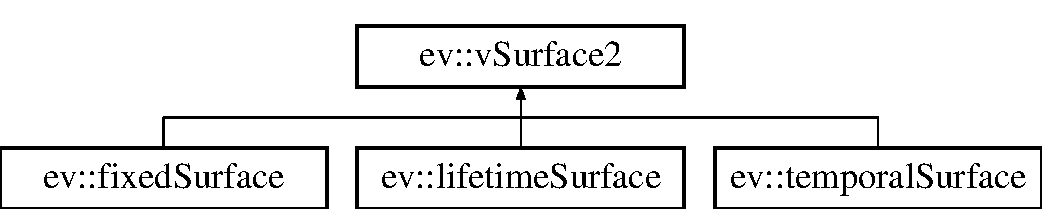
\includegraphics[height=2.000000cm]{classev_1_1vSurface2}
\end{center}
\end{figure}
\subsection*{Public Member Functions}
\begin{DoxyCompactItemize}
\item 
\hyperlink{classev_1_1vSurface2_ada6aeb852479aa111b1f5ad32ac1286b}{v\+Surface2} (int \hyperlink{classev_1_1vSurface2_a1aa8027816352a15d5b9bf1f26f48e76}{width}=128, int height=128)
\begin{DoxyCompactList}\small\item\em v\+Window constructor \end{DoxyCompactList}\item 
virtual \hyperlink{classev_1_1vQueue}{v\+Queue} \hyperlink{classev_1_1vSurface2_a6dee662976048b73d7b19e45871352da}{add\+Event} (event$<$$>$ v)
\begin{DoxyCompactList}\small\item\em add\+Event adds an event to the window. Also checks for expired events. \end{DoxyCompactList}\item 
virtual \hyperlink{classev_1_1vQueue}{v\+Queue} {\bfseries remove\+Events} (event$<$$>$ to\+Add)=0\hypertarget{classev_1_1vSurface2_af35870c14a5c94dc7522bdfcf76df2cb}{}\label{classev_1_1vSurface2_af35870c14a5c94dc7522bdfcf76df2cb}

\item 
event \hyperlink{classev_1_1vSurface2_af84a860e057aea43831e8e6d16107cd4}{get\+Most\+Recent} ()
\begin{DoxyCompactList}\small\item\em get\+Most\+Recent \end{DoxyCompactList}\item 
int {\bfseries get\+Event\+Count} ()\hypertarget{classev_1_1vSurface2_a67906f1ecd7fab30f1d0f7218388234e}{}\label{classev_1_1vSurface2_a67906f1ecd7fab30f1d0f7218388234e}

\item 
\hyperlink{classev_1_1vQueue}{v\+Queue} \hyperlink{classev_1_1vSurface2_aedcc28d0ccdbc343f031506a8fa84bb0}{get\+Surf} ()
\begin{DoxyCompactList}\small\item\em get\+Window \end{DoxyCompactList}\item 
\hyperlink{classev_1_1vQueue}{v\+Queue} {\bfseries get\+Surf} (int d)\hypertarget{classev_1_1vSurface2_aaa5978b3d040e278db563495585adf86}{}\label{classev_1_1vSurface2_aaa5978b3d040e278db563495585adf86}

\item 
\hyperlink{classev_1_1vQueue}{v\+Queue} \hyperlink{classev_1_1vSurface2_a42f7a69a075225254ffddc7bb5d4d9ba}{get\+Surf} (int x, int y, int d)
\begin{DoxyCompactList}\small\item\em get\+Spatial\+Window returns Address\+Events within a spatial window \end{DoxyCompactList}\item 
\hyperlink{classev_1_1vQueue}{v\+Queue} \hyperlink{classev_1_1vSurface2_aa74adc0c56d62a6f51c2901ec209233e}{get\+Surf} (int xl, int xh, int yl, int yh)
\begin{DoxyCompactList}\small\item\em get\+Spatial\+Window returns Address\+Events within a spatial window \end{DoxyCompactList}\item 
\hyperlink{classev_1_1vQueue}{v\+Queue} {\bfseries get\+Surf\+\_\+\+Tlim} (int dt)\hypertarget{classev_1_1vSurface2_a70e292820956b12c3bc123c4e724e90a}{}\label{classev_1_1vSurface2_a70e292820956b12c3bc123c4e724e90a}

\item 
\hyperlink{classev_1_1vQueue}{v\+Queue} {\bfseries get\+Surf\+\_\+\+Tlim} (int dt, int d)\hypertarget{classev_1_1vSurface2_ad487a13d9bcd8433489fb7e7b3fa5dc8}{}\label{classev_1_1vSurface2_ad487a13d9bcd8433489fb7e7b3fa5dc8}

\item 
\hyperlink{classev_1_1vQueue}{v\+Queue} {\bfseries get\+Surf\+\_\+\+Tlim} (int dt, int x, int y, int d)\hypertarget{classev_1_1vSurface2_a53939fc4b201eaee766114982d0ae9c2}{}\label{classev_1_1vSurface2_a53939fc4b201eaee766114982d0ae9c2}

\item 
\hyperlink{classev_1_1vQueue}{v\+Queue} {\bfseries get\+Surf\+\_\+\+Tlim} (int dt, int xl, int xh, int yl, int yh)\hypertarget{classev_1_1vSurface2_a63c601ec2570dbde037c9ea92342b24b}{}\label{classev_1_1vSurface2_a63c601ec2570dbde037c9ea92342b24b}

\item 
\hyperlink{classev_1_1vQueue}{v\+Queue} {\bfseries get\+Surf\+\_\+\+Clim} (int c)\hypertarget{classev_1_1vSurface2_acb41c1eff67ff285be715f8504d37d22}{}\label{classev_1_1vSurface2_acb41c1eff67ff285be715f8504d37d22}

\item 
\hyperlink{classev_1_1vQueue}{v\+Queue} {\bfseries get\+Surf\+\_\+\+Clim} (int c, int d)\hypertarget{classev_1_1vSurface2_af9e9a30828d508f49921b02224723a36}{}\label{classev_1_1vSurface2_af9e9a30828d508f49921b02224723a36}

\item 
\hyperlink{classev_1_1vQueue}{v\+Queue} {\bfseries get\+Surf\+\_\+\+Clim} (int c, int x, int y, int d)\hypertarget{classev_1_1vSurface2_a708416f0ae3b13858f1c96e203898223}{}\label{classev_1_1vSurface2_a708416f0ae3b13858f1c96e203898223}

\item 
\hyperlink{classev_1_1vQueue}{v\+Queue} {\bfseries get\+Surf\+\_\+\+Clim} (int c, int xl, int xh, int yl, int yh)\hypertarget{classev_1_1vSurface2_a1b04ff8d8d449b054a514c092bac1145}{}\label{classev_1_1vSurface2_a1b04ff8d8d449b054a514c092bac1145}

\end{DoxyCompactItemize}
\subsection*{Protected Attributes}
\begin{DoxyCompactItemize}
\item 
\hyperlink{classev_1_1vQueue}{v\+Queue} \hyperlink{classev_1_1vSurface2_ad26e2a77d859924e39526fe69ad6e8bf}{q}\hypertarget{classev_1_1vSurface2_ad26e2a77d859924e39526fe69ad6e8bf}{}\label{classev_1_1vSurface2_ad26e2a77d859924e39526fe69ad6e8bf}

\begin{DoxyCompactList}\small\item\em event storage \end{DoxyCompactList}\item 
std\+::vector$<$ std\+::vector$<$ event$<$$>$ $>$ $>$ \hyperlink{classev_1_1vSurface2_aeea3647a3da9c08bd0f3bd577e6ba443}{spatial}\hypertarget{classev_1_1vSurface2_aeea3647a3da9c08bd0f3bd577e6ba443}{}\label{classev_1_1vSurface2_aeea3647a3da9c08bd0f3bd577e6ba443}

\begin{DoxyCompactList}\small\item\em for quick spatial accessing and surfacing \end{DoxyCompactList}\item 
int \hyperlink{classev_1_1vSurface2_a1aa8027816352a15d5b9bf1f26f48e76}{width}\hypertarget{classev_1_1vSurface2_a1aa8027816352a15d5b9bf1f26f48e76}{}\label{classev_1_1vSurface2_a1aa8027816352a15d5b9bf1f26f48e76}

\begin{DoxyCompactList}\small\item\em retina size \end{DoxyCompactList}\item 
int {\bfseries height}\hypertarget{classev_1_1vSurface2_a4cac3483eefdbe9e83ced2ef6bc5f7b2}{}\label{classev_1_1vSurface2_a4cac3483eefdbe9e83ced2ef6bc5f7b2}

\item 
int \hyperlink{classev_1_1vSurface2_a53cfa9932bf60007440cbf535c115222}{count}\hypertarget{classev_1_1vSurface2_a53cfa9932bf60007440cbf535c115222}{}\label{classev_1_1vSurface2_a53cfa9932bf60007440cbf535c115222}

\begin{DoxyCompactList}\small\item\em active events \end{DoxyCompactList}\end{DoxyCompactItemize}


\subsection{Detailed Description}
The v\+Window class holds a list of events for a period of time as specified. Event expiry is checked each time new events are added and expired events are removed. At any point in time a copy of the current list of events can be requested. 

\subsection{Constructor \& Destructor Documentation}
\index{ev\+::v\+Surface2@{ev\+::v\+Surface2}!v\+Surface2@{v\+Surface2}}
\index{v\+Surface2@{v\+Surface2}!ev\+::v\+Surface2@{ev\+::v\+Surface2}}
\subsubsection[{\texorpdfstring{v\+Surface2(int width=128, int height=128)}{vSurface2(int width=128, int height=128)}}]{\setlength{\rightskip}{0pt plus 5cm}ev\+::v\+Surface2\+::v\+Surface2 (
\begin{DoxyParamCaption}
\item[{int}]{width = {\ttfamily 128}, }
\item[{int}]{height = {\ttfamily 128}}
\end{DoxyParamCaption}
)}\hypertarget{classev_1_1vSurface2_ada6aeb852479aa111b1f5ad32ac1286b}{}\label{classev_1_1vSurface2_ada6aeb852479aa111b1f5ad32ac1286b}


v\+Window constructor 


\begin{DoxyParams}{Parameters}
{\em window\+Size} & optional time to store events (in us) \\
\hline
\end{DoxyParams}


\subsection{Member Function Documentation}
\index{ev\+::v\+Surface2@{ev\+::v\+Surface2}!add\+Event@{add\+Event}}
\index{add\+Event@{add\+Event}!ev\+::v\+Surface2@{ev\+::v\+Surface2}}
\subsubsection[{\texorpdfstring{add\+Event(event$<$$>$ v)}{addEvent(event<> v)}}]{\setlength{\rightskip}{0pt plus 5cm}{\bf v\+Queue} ev\+::v\+Surface2\+::add\+Event (
\begin{DoxyParamCaption}
\item[{event$<$$>$}]{v}
\end{DoxyParamCaption}
)\hspace{0.3cm}{\ttfamily [virtual]}}\hypertarget{classev_1_1vSurface2_a6dee662976048b73d7b19e45871352da}{}\label{classev_1_1vSurface2_a6dee662976048b73d7b19e45871352da}


add\+Event adds an event to the window. Also checks for expired events. 


\begin{DoxyParams}{Parameters}
{\em event} & the event to add \\
\hline
\end{DoxyParams}


Reimplemented in \hyperlink{classev_1_1lifetimeSurface_a8fce037a13281c0e46c7d660e0ea2275}{ev\+::lifetime\+Surface}.

\index{ev\+::v\+Surface2@{ev\+::v\+Surface2}!get\+Most\+Recent@{get\+Most\+Recent}}
\index{get\+Most\+Recent@{get\+Most\+Recent}!ev\+::v\+Surface2@{ev\+::v\+Surface2}}
\subsubsection[{\texorpdfstring{get\+Most\+Recent()}{getMostRecent()}}]{\setlength{\rightskip}{0pt plus 5cm}event ev\+::v\+Surface2\+::get\+Most\+Recent (
\begin{DoxyParamCaption}
{}
\end{DoxyParamCaption}
)}\hypertarget{classev_1_1vSurface2_af84a860e057aea43831e8e6d16107cd4}{}\label{classev_1_1vSurface2_af84a860e057aea43831e8e6d16107cd4}


get\+Most\+Recent 

\begin{DoxyReturn}{Returns}

\end{DoxyReturn}
\index{ev\+::v\+Surface2@{ev\+::v\+Surface2}!get\+Surf@{get\+Surf}}
\index{get\+Surf@{get\+Surf}!ev\+::v\+Surface2@{ev\+::v\+Surface2}}
\subsubsection[{\texorpdfstring{get\+Surf()}{getSurf()}}]{\setlength{\rightskip}{0pt plus 5cm}{\bf v\+Queue} ev\+::v\+Surface2\+::get\+Surf (
\begin{DoxyParamCaption}
{}
\end{DoxyParamCaption}
)}\hypertarget{classev_1_1vSurface2_aedcc28d0ccdbc343f031506a8fa84bb0}{}\label{classev_1_1vSurface2_aedcc28d0ccdbc343f031506a8fa84bb0}


get\+Window 

\begin{DoxyReturn}{Returns}

\end{DoxyReturn}
\index{ev\+::v\+Surface2@{ev\+::v\+Surface2}!get\+Surf@{get\+Surf}}
\index{get\+Surf@{get\+Surf}!ev\+::v\+Surface2@{ev\+::v\+Surface2}}
\subsubsection[{\texorpdfstring{get\+Surf(int x, int y, int d)}{getSurf(int x, int y, int d)}}]{\setlength{\rightskip}{0pt plus 5cm}{\bf v\+Queue} ev\+::v\+Surface2\+::get\+Surf (
\begin{DoxyParamCaption}
\item[{int}]{x, }
\item[{int}]{y, }
\item[{int}]{d}
\end{DoxyParamCaption}
)}\hypertarget{classev_1_1vSurface2_a42f7a69a075225254ffddc7bb5d4d9ba}{}\label{classev_1_1vSurface2_a42f7a69a075225254ffddc7bb5d4d9ba}


get\+Spatial\+Window returns Address\+Events within a spatial window 


\begin{DoxyParams}{Parameters}
{\em x} & x centre \\
\hline
{\em y} & y centre \\
\hline
{\em d} & distance of the half-\/length of a square window \\
\hline
\end{DoxyParams}
\begin{DoxyReturn}{Returns}
a \hyperlink{classev_1_1vQueue}{v\+Queue} containing a copy of the events 
\end{DoxyReturn}
\index{ev\+::v\+Surface2@{ev\+::v\+Surface2}!get\+Surf@{get\+Surf}}
\index{get\+Surf@{get\+Surf}!ev\+::v\+Surface2@{ev\+::v\+Surface2}}
\subsubsection[{\texorpdfstring{get\+Surf(int xl, int xh, int yl, int yh)}{getSurf(int xl, int xh, int yl, int yh)}}]{\setlength{\rightskip}{0pt plus 5cm}{\bf v\+Queue} ev\+::v\+Surface2\+::get\+Surf (
\begin{DoxyParamCaption}
\item[{int}]{xl, }
\item[{int}]{xh, }
\item[{int}]{yl, }
\item[{int}]{yh}
\end{DoxyParamCaption}
)}\hypertarget{classev_1_1vSurface2_aa74adc0c56d62a6f51c2901ec209233e}{}\label{classev_1_1vSurface2_aa74adc0c56d62a6f51c2901ec209233e}


get\+Spatial\+Window returns Address\+Events within a spatial window 


\begin{DoxyParams}{Parameters}
{\em xl} & lower x value of window \\
\hline
{\em xh} & upper x value of window \\
\hline
{\em yl} & lower y value of window \\
\hline
{\em yh} & upper y value of window \\
\hline
\end{DoxyParams}
\begin{DoxyReturn}{Returns}
a \hyperlink{classev_1_1vQueue}{v\+Queue} containing a copy of the events 
\end{DoxyReturn}


The documentation for this class was generated from the following files\+:\begin{DoxyCompactItemize}
\item 
/home/aglover/workspace/projects/event-\/driven/libraries/include/i\+Cub/eventdriven/v\+Window.\+h\item 
/home/aglover/workspace/projects/event-\/driven/libraries/src/v\+Window.\+cpp\end{DoxyCompactItemize}

\hypertarget{classvSurfaceHandler}{}\section{v\+Surface\+Handler Class Reference}
\label{classvSurfaceHandler}\index{v\+Surface\+Handler@{v\+Surface\+Handler}}
Inheritance diagram for v\+Surface\+Handler\+:\begin{figure}[H]
\begin{center}
\leavevmode
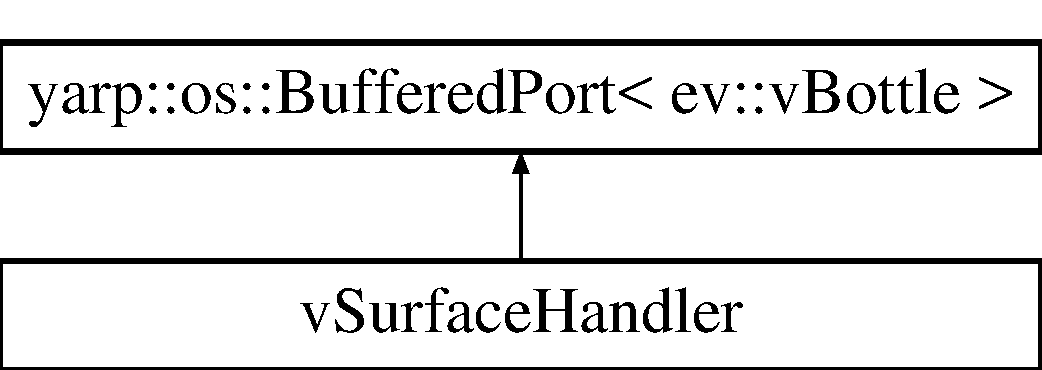
\includegraphics[height=2.000000cm]{classvSurfaceHandler}
\end{center}
\end{figure}
\subsection*{Public Member Functions}
\begin{DoxyCompactItemize}
\item 
{\bfseries v\+Surface\+Handler} (unsigned int width=128, unsigned int height=128)\hypertarget{classvSurfaceHandler_a9f1381af78c147b148fa1df4c7d4aebc}{}\label{classvSurfaceHandler_a9f1381af78c147b148fa1df4c7d4aebc}

\item 
void {\bfseries resize} (unsigned int width, unsigned int height)\hypertarget{classvSurfaceHandler_a391db0c36a4af25b7a33cb60c1f7a73b}{}\label{classvSurfaceHandler_a391db0c36a4af25b7a33cb60c1f7a73b}

\item 
\hyperlink{classev_1_1vQueue}{ev\+::v\+Queue} {\bfseries query\+Events} (unsigned long int condition\+Time, unsigned int temporal\+Window)\hypertarget{classvSurfaceHandler_a02ce8ea7ed25907c6c83cfd277748f7d}{}\label{classvSurfaceHandler_a02ce8ea7ed25907c6c83cfd277748f7d}

\item 
bool {\bfseries open} (const std\+::string \&name, bool strictness=false)\hypertarget{classvSurfaceHandler_ac8ec7581a0704b7dee1ad1265bf0fb9d}{}\label{classvSurfaceHandler_ac8ec7581a0704b7dee1ad1265bf0fb9d}

\item 
void {\bfseries on\+Read} (\hyperlink{classev_1_1vBottle}{ev\+::v\+Bottle} \&in\+Bot)\hypertarget{classvSurfaceHandler_a336eced82529cafe4bfc6e304d4aa074}{}\label{classvSurfaceHandler_a336eced82529cafe4bfc6e304d4aa074}

\item 
void {\bfseries close} ()\hypertarget{classvSurfaceHandler_adba8a4ac6f797f379ec06ef929857c81}{}\label{classvSurfaceHandler_adba8a4ac6f797f379ec06ef929857c81}

\item 
void {\bfseries interrupt} ()\hypertarget{classvSurfaceHandler_a1a6902fe50bd86981743a2af909d6073}{}\label{classvSurfaceHandler_a1a6902fe50bd86981743a2af909d6073}

\end{DoxyCompactItemize}


The documentation for this class was generated from the following files\+:\begin{DoxyCompactItemize}
\item 
/home/aglover/workspace/projects/event-\/driven/src/modules/v\+Particle\+Filter/include/v\+Particle\+Module.\+h\item 
/home/aglover/workspace/projects/event-\/driven/src/modules/v\+Particle\+Filter/src/v\+Particle\+Module.\+cpp\end{DoxyCompactItemize}

\hypertarget{classvTemplateModule}{}\section{v\+Template\+Module Class Reference}
\label{classvTemplateModule}\index{v\+Template\+Module@{v\+Template\+Module}}
Inheritance diagram for v\+Template\+Module\+:\begin{figure}[H]
\begin{center}
\leavevmode
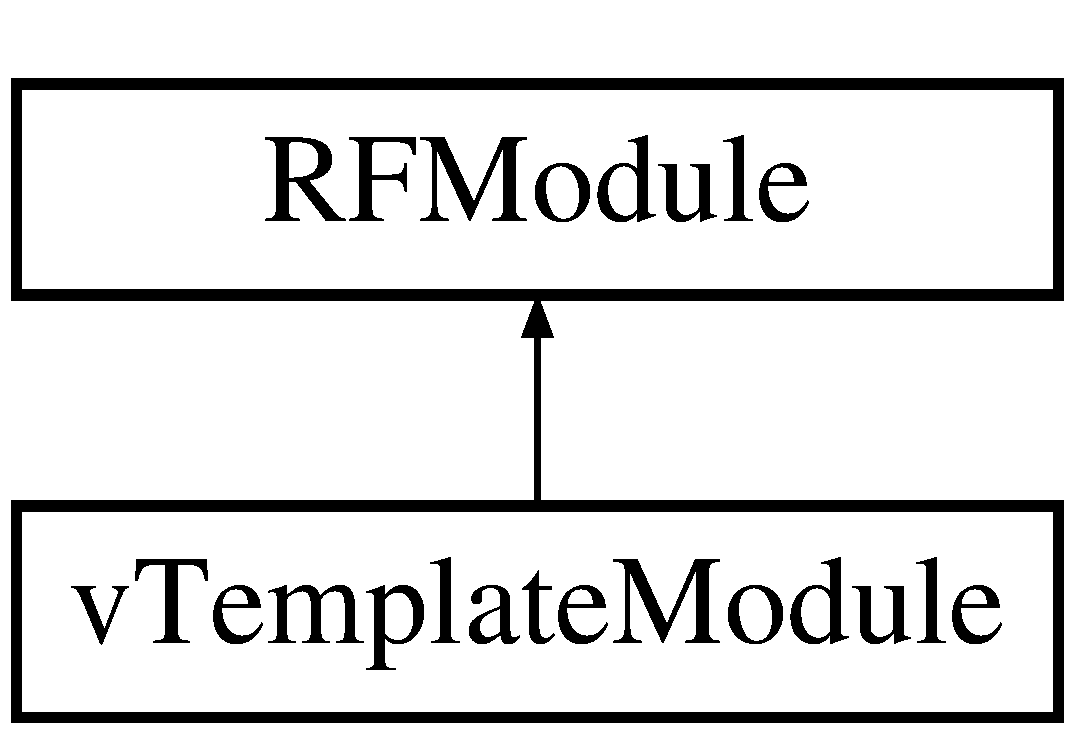
\includegraphics[height=2.000000cm]{classvTemplateModule}
\end{center}
\end{figure}
\subsection*{Public Member Functions}
\begin{DoxyCompactItemize}
\item 
virtual bool {\bfseries configure} (yarp\+::os\+::\+Resource\+Finder \&rf)\hypertarget{classvTemplateModule_ac673213dfbb34f1719a8a17b5549f3ab}{}\label{classvTemplateModule_ac673213dfbb34f1719a8a17b5549f3ab}

\item 
virtual bool {\bfseries interrupt\+Module} ()\hypertarget{classvTemplateModule_a4104e88622abbd133df02af82988a167}{}\label{classvTemplateModule_a4104e88622abbd133df02af82988a167}

\item 
virtual bool {\bfseries close} ()\hypertarget{classvTemplateModule_ac94b9d709bf56efac2a9f82f393843dc}{}\label{classvTemplateModule_ac94b9d709bf56efac2a9f82f393843dc}

\item 
virtual bool {\bfseries respond} (const yarp\+::os\+::\+Bottle \&command, yarp\+::os\+::\+Bottle \&reply)\hypertarget{classvTemplateModule_aa2e6141f31e4cea8f94f0b5a1b08a934}{}\label{classvTemplateModule_aa2e6141f31e4cea8f94f0b5a1b08a934}

\item 
virtual double {\bfseries get\+Period} ()\hypertarget{classvTemplateModule_a691e4424b5de4ee43e249421a24a87cb}{}\label{classvTemplateModule_a691e4424b5de4ee43e249421a24a87cb}

\item 
virtual bool {\bfseries update\+Module} ()\hypertarget{classvTemplateModule_abd78b6b36cc849bbc34d6a3033cc4654}{}\label{classvTemplateModule_abd78b6b36cc849bbc34d6a3033cc4654}

\end{DoxyCompactItemize}


The documentation for this class was generated from the following files\+:\begin{DoxyCompactItemize}
\item 
/home/aglover/workspace/projects/event-\/driven/src/modules/template/include/v\+Template.\+h\item 
/home/aglover/workspace/projects/event-\/driven/src/modules/template/src/v\+Template.\+cpp\end{DoxyCompactItemize}

\hypertarget{classev_1_1vTempWindow}{}\section{ev\+:\+:v\+Temp\+Window Class Reference}
\label{classev_1_1vTempWindow}\index{ev\+::v\+Temp\+Window@{ev\+::v\+Temp\+Window}}
\subsection*{Public Member Functions}
\begin{DoxyCompactItemize}
\item 
void {\bfseries add\+Event} (event$<$$>$ v)\hypertarget{classev_1_1vTempWindow_a9499371e18cc811e2cd3e47e8e96f8ca}{}\label{classev_1_1vTempWindow_a9499371e18cc811e2cd3e47e8e96f8ca}

\item 
void {\bfseries add\+Events} (const \hyperlink{classev_1_1vQueue}{v\+Queue} \&events)\hypertarget{classev_1_1vTempWindow_a925ee62f3dff9517654fd6a9a402616b}{}\label{classev_1_1vTempWindow_a925ee62f3dff9517654fd6a9a402616b}

\item 
\hyperlink{classev_1_1vQueue}{v\+Queue} {\bfseries get\+Window} ()\hypertarget{classev_1_1vTempWindow_a40ddfc12e259c028a57d5dd188b3e2e9}{}\label{classev_1_1vTempWindow_a40ddfc12e259c028a57d5dd188b3e2e9}

\end{DoxyCompactItemize}
\subsection*{Protected Attributes}
\begin{DoxyCompactItemize}
\item 
\hyperlink{classev_1_1vQueue}{v\+Queue} \hyperlink{classev_1_1vTempWindow_abed022ad51f68443a2350fbeabbb4233}{q}\hypertarget{classev_1_1vTempWindow_abed022ad51f68443a2350fbeabbb4233}{}\label{classev_1_1vTempWindow_abed022ad51f68443a2350fbeabbb4233}

\begin{DoxyCompactList}\small\item\em event storage \end{DoxyCompactList}\item 
int \hyperlink{classev_1_1vTempWindow_a909a8f6df0014d1f318c6209223f5fad}{t\+Upper}\hypertarget{classev_1_1vTempWindow_a909a8f6df0014d1f318c6209223f5fad}{}\label{classev_1_1vTempWindow_a909a8f6df0014d1f318c6209223f5fad}

\begin{DoxyCompactList}\small\item\em precalculated thresholds \end{DoxyCompactList}\item 
int {\bfseries t\+Lower}\hypertarget{classev_1_1vTempWindow_a47845a9e47b73598e2a325c06e994bed}{}\label{classev_1_1vTempWindow_a47845a9e47b73598e2a325c06e994bed}

\end{DoxyCompactItemize}


The documentation for this class was generated from the following files\+:\begin{DoxyCompactItemize}
\item 
/home/aglover/workspace/projects/event-\/driven/libraries/include/i\+Cub/eventdriven/v\+Window.\+h\item 
/home/aglover/workspace/projects/event-\/driven/libraries/src/v\+Temp\+Window.\+cpp\end{DoxyCompactItemize}

\hypertarget{classvTrackToRobotManager}{}\section{v\+Track\+To\+Robot\+Manager Class Reference}
\label{classvTrackToRobotManager}\index{v\+Track\+To\+Robot\+Manager@{v\+Track\+To\+Robot\+Manager}}
Inheritance diagram for v\+Track\+To\+Robot\+Manager\+:\begin{figure}[H]
\begin{center}
\leavevmode
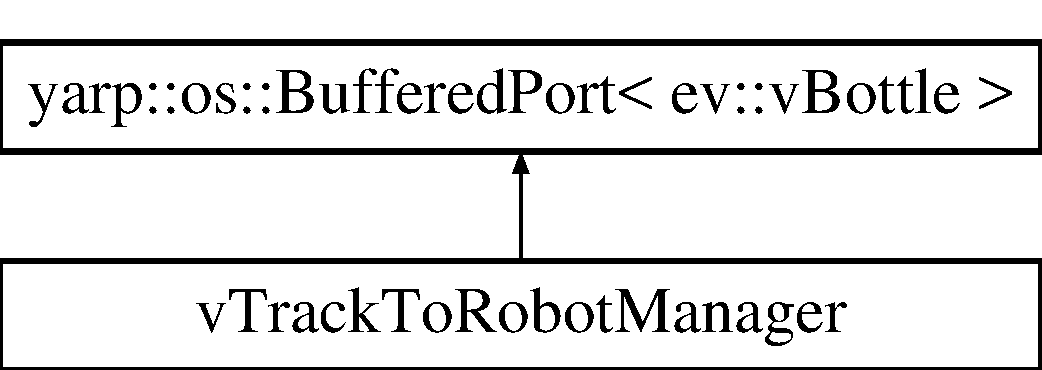
\includegraphics[height=2.000000cm]{classvTrackToRobotManager}
\end{center}
\end{figure}
\subsection*{Public Member Functions}
\begin{DoxyCompactItemize}
\item 
void {\bfseries set\+Method} (std\+::string methodname)\hypertarget{classvTrackToRobotManager_ada1644880b4c6f127e79a440bf5ed9f3}{}\label{classvTrackToRobotManager_ada1644880b4c6f127e79a440bf5ed9f3}

\item 
void {\bfseries set\+Demo} (std\+::string demoname)\hypertarget{classvTrackToRobotManager_ae30c22fd31a7c8bcef72aec0462db7fa}{}\label{classvTrackToRobotManager_ae30c22fd31a7c8bcef72aec0462db7fa}

\item 
void {\bfseries start\+Gazing} ()\hypertarget{classvTrackToRobotManager_a5989c99917c5dba694b2eeae5dcc4af8}{}\label{classvTrackToRobotManager_a5989c99917c5dba694b2eeae5dcc4af8}

\item 
void {\bfseries stop\+Gazing} ()\hypertarget{classvTrackToRobotManager_abb4dd1f6e4965be867aabeccc8674056}{}\label{classvTrackToRobotManager_abb4dd1f6e4965be867aabeccc8674056}

\item 
bool {\bfseries open} (const std\+::string \&name)\hypertarget{classvTrackToRobotManager_acd829a9e8130d24812666a2738926468}{}\label{classvTrackToRobotManager_acd829a9e8130d24812666a2738926468}

\item 
void {\bfseries on\+Read} (\hyperlink{classev_1_1vBottle}{ev\+::v\+Bottle} \&bot)\hypertarget{classvTrackToRobotManager_a8ba3d4d747e4691bf3dc8724aa69569c}{}\label{classvTrackToRobotManager_a8ba3d4d747e4691bf3dc8724aa69569c}

\item 
void {\bfseries interrupt} ()\hypertarget{classvTrackToRobotManager_a3d413d0808aeef12be32541cd2e892ed}{}\label{classvTrackToRobotManager_a3d413d0808aeef12be32541cd2e892ed}

\item 
void {\bfseries close} ()\hypertarget{classvTrackToRobotManager_a2d43766cdec75aa97d064276c17ee81c}{}\label{classvTrackToRobotManager_a2d43766cdec75aa97d064276c17ee81c}

\end{DoxyCompactItemize}


The documentation for this class was generated from the following files\+:\begin{DoxyCompactItemize}
\item 
/home/aglover/workspace/projects/event-\/driven/src/robotio/v\+Track\+To\+Robot/include/v\+Track\+To\+Robot.\+h\item 
/home/aglover/workspace/projects/event-\/driven/src/robotio/v\+Track\+To\+Robot/src/v\+Track\+To\+Robot.\+cpp\end{DoxyCompactItemize}

\hypertarget{classvTrackToRobotModule}{}\section{v\+Track\+To\+Robot\+Module Class Reference}
\label{classvTrackToRobotModule}\index{v\+Track\+To\+Robot\+Module@{v\+Track\+To\+Robot\+Module}}
Inheritance diagram for v\+Track\+To\+Robot\+Module\+:\begin{figure}[H]
\begin{center}
\leavevmode
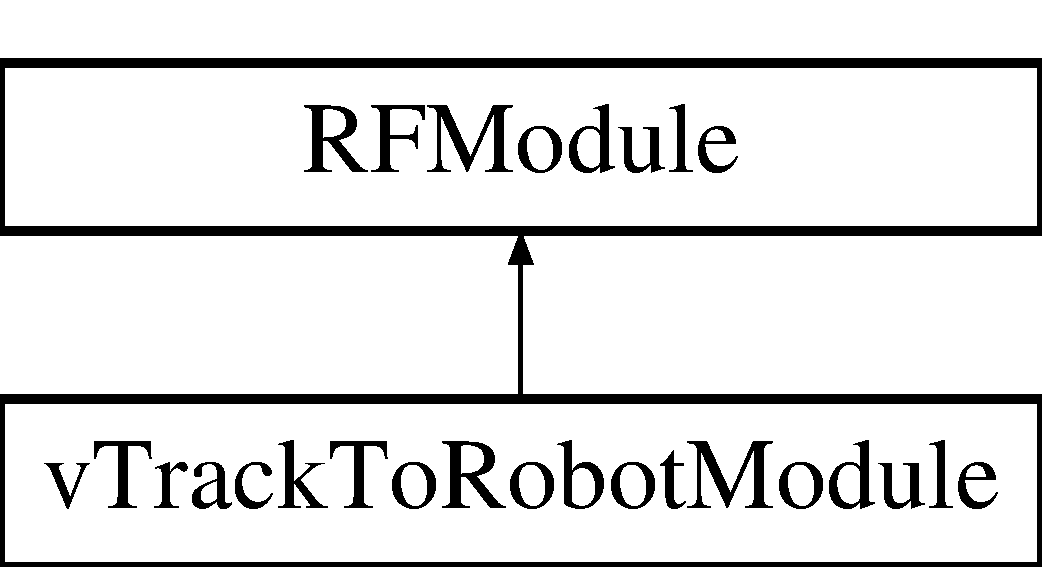
\includegraphics[height=2.000000cm]{classvTrackToRobotModule}
\end{center}
\end{figure}
\subsection*{Public Member Functions}
\begin{DoxyCompactItemize}
\item 
virtual bool {\bfseries configure} (yarp\+::os\+::\+Resource\+Finder \&rf)\hypertarget{classvTrackToRobotModule_ac724b3b5b9a538f211b062d2adf0118d}{}\label{classvTrackToRobotModule_ac724b3b5b9a538f211b062d2adf0118d}

\item 
virtual bool {\bfseries interrupt\+Module} ()\hypertarget{classvTrackToRobotModule_a83db4c48a68b502cc18b8a2ddad56f31}{}\label{classvTrackToRobotModule_a83db4c48a68b502cc18b8a2ddad56f31}

\item 
virtual bool {\bfseries close} ()\hypertarget{classvTrackToRobotModule_af9d2b13bb4c006718d62a354f96a559a}{}\label{classvTrackToRobotModule_af9d2b13bb4c006718d62a354f96a559a}

\item 
virtual double {\bfseries get\+Period} ()\hypertarget{classvTrackToRobotModule_adcd051ae7fa4bec4cc8dd121c1f85931}{}\label{classvTrackToRobotModule_adcd051ae7fa4bec4cc8dd121c1f85931}

\item 
virtual bool {\bfseries update\+Module} ()\hypertarget{classvTrackToRobotModule_a6cb66f0717a055864f7ab4f8f0d8c132}{}\label{classvTrackToRobotModule_a6cb66f0717a055864f7ab4f8f0d8c132}

\item 
virtual bool {\bfseries respond} (const yarp\+::os\+::\+Bottle \&command, yarp\+::os\+::\+Bottle \&reply)\hypertarget{classvTrackToRobotModule_af14c10f5261e4a7790f35872f7e81361}{}\label{classvTrackToRobotModule_af14c10f5261e4a7790f35872f7e81361}

\end{DoxyCompactItemize}


The documentation for this class was generated from the following files\+:\begin{DoxyCompactItemize}
\item 
/home/aglover/workspace/projects/event-\/driven/src/robotio/v\+Track\+To\+Robot/include/v\+Track\+To\+Robot.\+h\item 
/home/aglover/workspace/projects/event-\/driven/src/robotio/v\+Track\+To\+Robot/src/v\+Track\+To\+Robot.\+cpp\end{DoxyCompactItemize}

\hypertarget{classev_1_1vtsHelper}{}\section{ev\+:\+:vts\+Helper Class Reference}
\label{classev_1_1vtsHelper}\index{ev\+::vts\+Helper@{ev\+::vts\+Helper}}
\subsection*{Public Member Functions}
\begin{DoxyCompactItemize}
\item 
unsigned long int {\bfseries operator()} (int timestamp)\hypertarget{classev_1_1vtsHelper_a399c3a719f7544209ba77f442c97c135}{}\label{classev_1_1vtsHelper_a399c3a719f7544209ba77f442c97c135}

\item 
unsigned long int {\bfseries current\+Time} ()\hypertarget{classev_1_1vtsHelper_ab8b7f4f4240f2a0f0279bda5f5f2caff}{}\label{classev_1_1vtsHelper_ab8b7f4f4240f2a0f0279bda5f5f2caff}

\end{DoxyCompactItemize}
\subsection*{Static Public Member Functions}
\begin{DoxyCompactItemize}
\item 
static long int {\bfseries max\+Stamp} ()\hypertarget{classev_1_1vtsHelper_aa7f1c13eb051773e9413b52bb52caad0}{}\label{classev_1_1vtsHelper_aa7f1c13eb051773e9413b52bb52caad0}

\item 
static double {\bfseries tstosecs} ()\hypertarget{classev_1_1vtsHelper_a07d0dc3cd7743eff7d594e838ae23a01}{}\label{classev_1_1vtsHelper_a07d0dc3cd7743eff7d594e838ae23a01}

\end{DoxyCompactItemize}


The documentation for this class was generated from the following file\+:\begin{DoxyCompactItemize}
\item 
/home/aglover/workspace/projects/event-\/driven/libraries/include/i\+Cub/eventdriven/vts\+Helper.\+h\end{DoxyCompactItemize}

\hypertarget{classyarp2device}{}\section{yarp2device Class Reference}
\label{classyarp2device}\index{yarp2device@{yarp2device}}
Inheritance diagram for yarp2device\+:\begin{figure}[H]
\begin{center}
\leavevmode
\includegraphics[height=2.000000cm]{classyarp2device}
\end{center}
\end{figure}
\subsection*{Public Member Functions}
\begin{DoxyCompactItemize}
\item 
bool {\bfseries initialise} (std\+::string module\+Name, std\+::string device\+Name)\hypertarget{classyarp2device_ab25c91e26d75cad2b01544040aa46b7b}{}\label{classyarp2device_ab25c91e26d75cad2b01544040aa46b7b}

\item 
bool {\bfseries init} ()\hypertarget{classyarp2device_a56b9560746d5dec6168f62426b302598}{}\label{classyarp2device_a56b9560746d5dec6168f62426b302598}

\item 
void {\bfseries close} ()\hypertarget{classyarp2device_a4031dba4c05576ca4f444fe496fd1f42}{}\label{classyarp2device_a4031dba4c05576ca4f444fe496fd1f42}

\item 
void {\bfseries on\+Read} (\hyperlink{classev_1_1vBottle}{ev\+::v\+Bottle} \&bot)\hypertarget{classyarp2device_a52d2819114122ec00c41b31b2842c608}{}\label{classyarp2device_a52d2819114122ec00c41b31b2842c608}

\item 
void {\bfseries interrupt} ()\hypertarget{classyarp2device_ad2c4ae1fdb9839805c806d0084fdd20a}{}\label{classyarp2device_ad2c4ae1fdb9839805c806d0084fdd20a}

\end{DoxyCompactItemize}


The documentation for this class was generated from the following files\+:\begin{DoxyCompactItemize}
\item 
/home/aglover/workspace/projects/event-\/driven/src/hardwareio/zynq\+Grabber/include/yarp\+Interface.\+h\item 
/home/aglover/workspace/projects/event-\/driven/src/hardwareio/zynq\+Grabber/src/yarp\+Interface.\+cpp\end{DoxyCompactItemize}

\hypertarget{classYARPsalientI}{}\section{Y\+A\+R\+PsalientI Class Reference}
\label{classYARPsalientI}\index{Y\+A\+R\+PsalientI@{Y\+A\+R\+PsalientI}}
Inheritance diagram for Y\+A\+R\+PsalientI\+:\begin{figure}[H]
\begin{center}
\leavevmode
\includegraphics[height=2.000000cm]{classYARPsalientI}
\end{center}
\end{figure}
\subsection*{Public Member Functions}
\begin{DoxyCompactItemize}
\item 
bool {\bfseries open} (const std\+::string \&name)\hypertarget{classYARPsalientI_a250043be66377743478e388938d74360}{}\label{classYARPsalientI_a250043be66377743478e388938d74360}

\item 
void {\bfseries close} ()\hypertarget{classYARPsalientI_a253d99f4b7595c0f314c6e85bd55073f}{}\label{classYARPsalientI_a253d99f4b7595c0f314c6e85bd55073f}

\item 
void {\bfseries interrupt} ()\hypertarget{classYARPsalientI_a17ab82fc3d6e2c463d62a5dcc17d8ea3}{}\label{classYARPsalientI_a17ab82fc3d6e2c463d62a5dcc17d8ea3}

\item 
void {\bfseries on\+Read} (emorph\+::v\+Bottle \&bot)\hypertarget{classYARPsalientI_ab6bf391f4c8ce629536eca1302866989}{}\label{classYARPsalientI_ab6bf391f4c8ce629536eca1302866989}

\end{DoxyCompactItemize}


The documentation for this class was generated from the following files\+:\begin{DoxyCompactItemize}
\item 
/home/aglover/workspace/projects/event-\/driven/src/modules/salient\+Pos/include/salient\+Pos.\+h\item 
/home/aglover/workspace/projects/event-\/driven/src/modules/salient\+Pos/src/salient\+Pos.\+cpp\end{DoxyCompactItemize}

\hypertarget{classYARPspinI}{}\section{Y\+A\+R\+PspinI Class Reference}
\label{classYARPspinI}\index{Y\+A\+R\+PspinI@{Y\+A\+R\+PspinI}}
Inheritance diagram for Y\+A\+R\+PspinI\+:\begin{figure}[H]
\begin{center}
\leavevmode
\includegraphics[height=2.000000cm]{classYARPspinI}
\end{center}
\end{figure}
\subsection*{Public Member Functions}
\begin{DoxyCompactItemize}
\item 
bool {\bfseries open} (const std\+::string \&name)\hypertarget{classYARPspinI_a749cd07632d7e3cd08846457e2d6be2e}{}\label{classYARPspinI_a749cd07632d7e3cd08846457e2d6be2e}

\item 
void {\bfseries close} ()\hypertarget{classYARPspinI_a6955f4744c185dd870b32ad17ddd75ef}{}\label{classYARPspinI_a6955f4744c185dd870b32ad17ddd75ef}

\item 
void {\bfseries interrupt} ()\hypertarget{classYARPspinI_a9340f1b20136adad3392c155393506ac}{}\label{classYARPspinI_a9340f1b20136adad3392c155393506ac}

\item 
void {\bfseries attach\+E\+I\+E\+I\+O\+Sender} (spinnio\+::\+E\+I\+E\+I\+O\+Sender $\ast$)\hypertarget{classYARPspinI_a6480c2630a974de7af8501ef2e2b9068}{}\label{classYARPspinI_a6480c2630a974de7af8501ef2e2b9068}

\item 
void {\bfseries on\+Read} (\hyperlink{classev_1_1vBottle}{ev\+::v\+Bottle} \&bot)\hypertarget{classYARPspinI_af965467765329a090b8e5153b1f01112}{}\label{classYARPspinI_af965467765329a090b8e5153b1f01112}

\end{DoxyCompactItemize}


The documentation for this class was generated from the following files\+:\begin{DoxyCompactItemize}
\item 
/home/aglover/workspace/projects/event-\/driven/src/hardwareio/spinterface/include/spinterface.\+h\item 
/home/aglover/workspace/projects/event-\/driven/src/hardwareio/spinterface/src/spinterface.\+cpp\end{DoxyCompactItemize}

\hypertarget{classYARPspinIO}{}\section{Y\+A\+R\+Pspin\+IO Class Reference}
\label{classYARPspinIO}\index{Y\+A\+R\+Pspin\+IO@{Y\+A\+R\+Pspin\+IO}}
Inheritance diagram for Y\+A\+R\+Pspin\+IO\+:\begin{figure}[H]
\begin{center}
\leavevmode
\includegraphics[height=2.000000cm]{classYARPspinIO}
\end{center}
\end{figure}
\subsection*{Public Member Functions}
\begin{DoxyCompactItemize}
\item 
bool {\bfseries open} (const std\+::string \&name)\hypertarget{classYARPspinIO_ac99ae5b0b8d9308da9a8aa76dd8b7cf6}{}\label{classYARPspinIO_ac99ae5b0b8d9308da9a8aa76dd8b7cf6}

\item 
void {\bfseries close} ()\hypertarget{classYARPspinIO_afbaa4ae29db56e010b1801a9c428386b}{}\label{classYARPspinIO_afbaa4ae29db56e010b1801a9c428386b}

\item 
void {\bfseries interrupt} ()\hypertarget{classYARPspinIO_ad00a2c121cbd513dd32726a26b15bef6}{}\label{classYARPspinIO_ad00a2c121cbd513dd32726a26b15bef6}

\item 
void {\bfseries attach\+E\+I\+E\+I\+Omodules} (spinnio\+::\+E\+I\+E\+I\+O\+Sender $\ast$spin\+Sender\+Ptr, spinnio\+::\+E\+I\+E\+I\+O\+Receiver $\ast$spin\+Receiver\+Ptr)\hypertarget{classYARPspinIO_af51eb6763550906becdf20b596c0adf9}{}\label{classYARPspinIO_af51eb6763550906becdf20b596c0adf9}

\item 
void {\bfseries on\+Read} (\hyperlink{classev_1_1vBottle}{ev\+::v\+Bottle} \&inbottle)\hypertarget{classYARPspinIO_a6f6002f899bdee449f5a695ac6f45dcb}{}\label{classYARPspinIO_a6f6002f899bdee449f5a695ac6f45dcb}

\end{DoxyCompactItemize}


The documentation for this class was generated from the following files\+:\begin{DoxyCompactItemize}
\item 
/home/aglover/workspace/projects/event-\/driven/src/hardwareio/spinterface/include/spinterface.\+h\item 
/home/aglover/workspace/projects/event-\/driven/src/hardwareio/spinterface/src/spinterface.\+cpp\end{DoxyCompactItemize}

\hypertarget{classYARPspinO}{}\section{Y\+A\+R\+PspinO Class Reference}
\label{classYARPspinO}\index{Y\+A\+R\+PspinO@{Y\+A\+R\+PspinO}}
Inheritance diagram for Y\+A\+R\+PspinO\+:\begin{figure}[H]
\begin{center}
\leavevmode
\includegraphics[height=2.000000cm]{classYARPspinO}
\end{center}
\end{figure}
\subsection*{Public Member Functions}
\begin{DoxyCompactItemize}
\item 
bool {\bfseries init\+Thread} (std\+::string module\+Name, spinnio\+::\+E\+I\+E\+I\+O\+Receiver $\ast$spin\+Receiver\+Ptr)\hypertarget{classYARPspinO_a6c43538e8a723f5d737b6bb7b67f6552}{}\label{classYARPspinO_a6c43538e8a723f5d737b6bb7b67f6552}

\item 
void {\bfseries run} ()\hypertarget{classYARPspinO_aff0148bb4f1b5a40122657ecc2cb7561}{}\label{classYARPspinO_aff0148bb4f1b5a40122657ecc2cb7561}

\item 
void {\bfseries thread\+Release} ()\hypertarget{classYARPspinO_a2e5c1ad532978c130c87b8159c2a3a0c}{}\label{classYARPspinO_a2e5c1ad532978c130c87b8159c2a3a0c}

\end{DoxyCompactItemize}


The documentation for this class was generated from the following files\+:\begin{DoxyCompactItemize}
\item 
/home/aglover/workspace/projects/event-\/driven/src/hardwareio/spinterface/include/spinterface.\+h\item 
/home/aglover/workspace/projects/event-\/driven/src/hardwareio/spinterface/src/spinterface.\+cpp\end{DoxyCompactItemize}

\hypertarget{classzynqGrabberModule}{}\section{zynq\+Grabber\+Module Class Reference}
\label{classzynqGrabberModule}\index{zynq\+Grabber\+Module@{zynq\+Grabber\+Module}}
Inheritance diagram for zynq\+Grabber\+Module\+:\begin{figure}[H]
\begin{center}
\leavevmode
\includegraphics[height=2.000000cm]{classzynqGrabberModule}
\end{center}
\end{figure}
\subsection*{Public Member Functions}
\begin{DoxyCompactItemize}
\item 
bool {\bfseries configure} (yarp\+::os\+::\+Resource\+Finder \&rf)\hypertarget{classzynqGrabberModule_a2733856709df020d264750ce5afbe552}{}\label{classzynqGrabberModule_a2733856709df020d264750ce5afbe552}

\item 
bool {\bfseries interrupt\+Module} ()\hypertarget{classzynqGrabberModule_aa33152e027843920826ea02f323df8dd}{}\label{classzynqGrabberModule_aa33152e027843920826ea02f323df8dd}

\item 
bool {\bfseries close} ()\hypertarget{classzynqGrabberModule_ae687b7063d3974a71a27a4cae8104480}{}\label{classzynqGrabberModule_ae687b7063d3974a71a27a4cae8104480}

\item 
bool {\bfseries respond} (const yarp\+::os\+::\+Bottle \&command, yarp\+::os\+::\+Bottle \&reply)\hypertarget{classzynqGrabberModule_afb439f66ef1786b6b503597dd6e74f33}{}\label{classzynqGrabberModule_afb439f66ef1786b6b503597dd6e74f33}

\item 
double {\bfseries get\+Period} ()\hypertarget{classzynqGrabberModule_a584429a662fd6eb0b11d77294c1b40a5}{}\label{classzynqGrabberModule_a584429a662fd6eb0b11d77294c1b40a5}

\item 
bool {\bfseries update\+Module} ()\hypertarget{classzynqGrabberModule_a53679eefbe74aa164fde84f9381450bc}{}\label{classzynqGrabberModule_a53679eefbe74aa164fde84f9381450bc}

\end{DoxyCompactItemize}


The documentation for this class was generated from the following files\+:\begin{DoxyCompactItemize}
\item 
/home/aglover/workspace/projects/event-\/driven/src/hardwareio/zynq\+Grabber/include/zynq\+Grabber\+Module.\+h\item 
/home/aglover/workspace/projects/event-\/driven/src/hardwareio/zynq\+Grabber/src/\hyperlink{zynqGrabberModule_8cpp}{zynq\+Grabber\+Module.\+cpp}\end{DoxyCompactItemize}

\chapter{File Documentation}
\hypertarget{config_8h}{}\section{/home/aglover/workspace/projects/event-\/driven/src/hardwareio/aex\+Grabber/include/config.h File Reference}
\label{config_8h}\index{/home/aglover/workspace/projects/event-\/driven/src/hardwareio/aex\+Grabber/include/config.\+h@{/home/aglover/workspace/projects/event-\/driven/src/hardwareio/aex\+Grabber/include/config.\+h}}


Simple header file for configuration. Intentionally separated for estetic purposes.  


\subsection*{Macros}
\begin{DoxyCompactItemize}
\item 
\#define {\bfseries S\+I\+Z\+E\+\_\+\+O\+F\+\_\+\+E\+V\+E\+NT}~2048\hypertarget{config_8h_ad49b36abd5473a87913e4964cc1564c9}{}\label{config_8h_ad49b36abd5473a87913e4964cc1564c9}

\item 
\#define {\bfseries S\+I\+Z\+E\+\_\+\+O\+F\+\_\+\+D\+A\+TA}~16384\hypertarget{config_8h_a458727ba44329288f712b89a0b52199a}{}\label{config_8h_a458727ba44329288f712b89a0b52199a}

\item 
\#define {\bfseries S\+L\+OW}\hypertarget{config_8h_a5da43425fff36347c69fc3c090e42c6c}{}\label{config_8h_a5da43425fff36347c69fc3c090e42c6c}

\end{DoxyCompactItemize}


\subsection{Detailed Description}
Simple header file for configuration. Intentionally separated for estetic purposes. 


\hypertarget{device2yarp_8h}{}\section{/home/aglover/workspace/projects/event-\/driven/src/hardwareio/aex\+Grabber/include/device2yarp.h File Reference}
\label{device2yarp_8h}\index{/home/aglover/workspace/projects/event-\/driven/src/hardwareio/aex\+Grabber/include/device2yarp.\+h@{/home/aglover/workspace/projects/event-\/driven/src/hardwareio/aex\+Grabber/include/device2yarp.\+h}}


Definition of the ratethread that receives events from D\+VS camera.  


{\ttfamily \#include $<$yarp/os/\+Rate\+Thread.\+h$>$}\\*
{\ttfamily \#include $<$yarp/os/\+Buffered\+Port.\+h$>$}\\*
{\ttfamily \#include $<$yarp/os/\+Semaphore.\+h$>$}\\*
{\ttfamily \#include $<$yarp/os/\+Bottle.\+h$>$}\\*
{\ttfamily \#include $<$yarp/os/\+Time.\+h$>$}\\*
{\ttfamily \#include $<$fcntl.\+h$>$}\\*
{\ttfamily \#include $<$sys/ioctl.\+h$>$}\\*
{\ttfamily \#include $<$iostream$>$}\\*
{\ttfamily \#include $<$sstream$>$}\\*
{\ttfamily \#include $<$cstdlib$>$}\\*
{\ttfamily \#include $<$stdint.\+h$>$}\\*
{\ttfamily \#include $<$fstream$>$}\\*
{\ttfamily \#include $<$i\+Cub/eventdriven/all.\+h$>$}\\*
\subsection*{Classes}
\begin{DoxyCompactItemize}
\item 
struct \hyperlink{structaer}{aer}
\item 
struct \hyperlink{structatom}{atom}
\item 
class \hyperlink{classdevice2yarp}{device2yarp}
\end{DoxyCompactItemize}
\subsection*{Macros}
\begin{DoxyCompactItemize}
\item 
\#define {\bfseries \+\_\+\+\_\+\+S\+T\+D\+C\+\_\+\+L\+I\+M\+I\+T\+\_\+\+M\+A\+C\+R\+OS}\hypertarget{device2yarp_8h_aeb7e7a856ab7a794b05b6b63ef36ea3e}{}\label{device2yarp_8h_aeb7e7a856ab7a794b05b6b63ef36ea3e}

\item 
\#define {\bfseries u8}~uint8\+\_\+t\hypertarget{device2yarp_8h_af3b86d961da0a3575b4f99c9ffaf01fd}{}\label{device2yarp_8h_af3b86d961da0a3575b4f99c9ffaf01fd}

\item 
\#define {\bfseries u16}~uint16\+\_\+t\hypertarget{device2yarp_8h_a2b19d553290a8d4a083d3c03280ea800}{}\label{device2yarp_8h_a2b19d553290a8d4a083d3c03280ea800}

\item 
\#define {\bfseries u32}~uint32\+\_\+t\hypertarget{device2yarp_8h_a332ccd83dfe2973e6cb2b61e4f3ab7e6}{}\label{device2yarp_8h_a332ccd83dfe2973e6cb2b61e4f3ab7e6}

\item 
\#define {\bfseries u64}~uint64\+\_\+t\hypertarget{device2yarp_8h_a969c7c1ebb4f70581e040a3034b14ee0}{}\label{device2yarp_8h_a969c7c1ebb4f70581e040a3034b14ee0}

\item 
\#define {\bfseries S\+I\+Z\+E\+\_\+\+O\+F\+\_\+\+E\+V\+E\+NT}~8192\hypertarget{device2yarp_8h_ad49b36abd5473a87913e4964cc1564c9}{}\label{device2yarp_8h_ad49b36abd5473a87913e4964cc1564c9}

\item 
\#define {\bfseries S\+I\+Z\+E\+\_\+\+O\+F\+\_\+\+D\+A\+TA}~65536\hypertarget{device2yarp_8h_a458727ba44329288f712b89a0b52199a}{}\label{device2yarp_8h_a458727ba44329288f712b89a0b52199a}

\end{DoxyCompactItemize}


\subsection{Detailed Description}
Definition of the ratethread that receives events from D\+VS camera. 


\hypertarget{sending__buffer_8h}{}\section{/home/aglover/workspace/projects/event-\/driven/src/hardwareio/aex\+Grabber/include/sending\+\_\+buffer.h File Reference}
\label{sending__buffer_8h}\index{/home/aglover/workspace/projects/event-\/driven/src/hardwareio/aex\+Grabber/include/sending\+\_\+buffer.\+h@{/home/aglover/workspace/projects/event-\/driven/src/hardwareio/aex\+Grabber/include/sending\+\_\+buffer.\+h}}


Sends the buffer (readings of cameras) on a Y\+A\+RP port.  


{\ttfamily \#include $<$yarp/os/\+Portable.\+h$>$}\\*
{\ttfamily \#include $<$yarp/os/\+Connection\+Writer.\+h$>$}\\*
{\ttfamily \#include $<$cstring$>$}\\*
{\ttfamily \#include \char`\"{}config.\+h\char`\"{}}\\*
\subsection*{Classes}
\begin{DoxyCompactItemize}
\item 
class \hyperlink{classsendingBuffer}{sending\+Buffer}
\end{DoxyCompactItemize}


\subsection{Detailed Description}
Sends the buffer (readings of cameras) on a Y\+A\+RP port. 

Sends information on a Y\+A\+RP port (see header \hyperlink{sending__buffer_8h}{sending\+\_\+buffer.\+h})
\hypertarget{aexGrabberModule_8cpp}{}\section{/home/aglover/workspace/projects/event-\/driven/src/hardwareio/aex\+Grabber/src/aex\+Grabber\+Module.cpp File Reference}
\label{aexGrabberModule_8cpp}\index{/home/aglover/workspace/projects/event-\/driven/src/hardwareio/aex\+Grabber/src/aex\+Grabber\+Module.\+cpp@{/home/aglover/workspace/projects/event-\/driven/src/hardwareio/aex\+Grabber/src/aex\+Grabber\+Module.\+cpp}}


Implementation of the \hyperlink{classaexGrabberModule}{aex\+Grabber\+Module} (see header file).  


{\ttfamily \#include $<$aex\+Grabber\+Module.\+h$>$}\\*


\subsection{Detailed Description}
Implementation of the \hyperlink{classaexGrabberModule}{aex\+Grabber\+Module} (see header file). 


\hypertarget{zynqGrabberModule_8cpp}{}\section{/home/aglover/workspace/projects/event-\/driven/src/hardwareio/zynq\+Grabber/src/zynq\+Grabber\+Module.cpp File Reference}
\label{zynqGrabberModule_8cpp}\index{/home/aglover/workspace/projects/event-\/driven/src/hardwareio/zynq\+Grabber/src/zynq\+Grabber\+Module.\+cpp@{/home/aglover/workspace/projects/event-\/driven/src/hardwareio/zynq\+Grabber/src/zynq\+Grabber\+Module.\+cpp}}


Implementation of the \hyperlink{classzynqGrabberModule}{zynq\+Grabber\+Module} (see header file).  


{\ttfamily \#include $<$zynq\+Grabber\+Module.\+h$>$}\\*


\subsection{Detailed Description}
Implementation of the \hyperlink{classzynqGrabberModule}{zynq\+Grabber\+Module} (see header file). 


%--- End generated contents ---

% Index
\backmatter
\newpage
\phantomsection
\clearemptydoublepage
\addcontentsline{toc}{chapter}{Index}
\printindex

\end{document}
